\documentclass[10pt,a4paper]{book}
\usepackage[utf8]{inputenc}
\usepackage[T1]{fontenc}
\usepackage{hyperref}
%\usepackage{natbib}
\usepackage[francais]{babel}
\usepackage{hyperref}
\usepackage{amssymb,amsthm,amsmath,amsfonts}
\usepackage{algorithm}
\usepackage{algorithmic}
\usepackage{units}
\usepackage{lmodern}
\usepackage{fp}
\usepackage{graphicx}
\usepackage{epsfig}
\usepackage{epstopdf}
\usepackage{makeidx}
\usepackage{gloss}
\usepackage{xcolor}
%\usepackage[toc]{glossaries}
\usepackage{changepage}
\usepackage{tikz}
\usepackage{array}
\usetikzlibrary{decorations}
\usetikzlibrary{decorations.pathreplacing}
\usetikzlibrary{calc}
\usetikzlibrary{fixedpointarithmetic}
\usepackage{todonotes}
\usepackage[intoc]{nomencl}
\usepackage{fancyhdr}
\pagestyle{fancy}
%\usepackage{apalike}
\usepackage{subfig}


\theoremstyle{plain}
\newtheorem{thm}{Théorème}[chapter]
\theoremstyle{definition} 
\newtheorem{lem}[thm]{Lemme}
\theoremstyle{definition} 
\newtheorem{cor}[thm]{Corollaire}
\theoremstyle{definition} 
\newtheorem{prop}[thm]{Proposition}
\theoremstyle{definition} 
\newtheorem{defi}[thm]{Définition}
\theoremstyle{remark} 
\newtheorem{rem}[thm]{Remarque}
\theoremstyle{remark} 
\newtheorem{exe}[thm]{Exemple}
\theoremstyle{definition}
\newtheorem{nota}[thm]{Notation}



\newcommand{\defeq}{\mathrel{\mathop:}=}

\author{Hugounenq Cyril}
\title{Volcans et calcul d'isogénies}
\makenomenclature
\makeindex



\makeatletter
\def\footrule{{
\vskip-\footruleskip\vskip-\footrulewidth
\color{\footrulecolor}
\hrule\@width\headwidth\@height
\footrulewidth\vskip\footruleskip
}}

\makeatother
%\makeglossaries
 
%\newglossaryentry{PI}{
%		name=$\pi$,
%		description={L'endomorphisme de Frobenius}% 
%		}

% 

\renewcommand{\nomname}{Nomenclature}
 
\renewcommand{\nompreamble}{La liste suivante décrit certains symboles qui seront utilisés tout au long de ce document.}

\bibliographystyle{alpha}
%%% BEGIN DOCUMENT
\begin{document}
\fancyhf{}%␣efface␣tout␣ce␣qu'il␣y␣avait␣avant
\fancyhead[L]{\nouppercase\leftmark}%␣LO␣=␣gauche/impair␣;␣RE␣=␣droite/pair
\fancyhead[R]{}
\fancyfoot[C]{\thepage}%␣C␣=␣centré
\fancyfoot[L]{}



\renewcommand{\headrulewidth}{1pt}% 1pt header rule
\renewcommand{\headrule}{\hbox to\headwidth{%
  \color{orange}\leaders\hrule height \headrulewidth\hfill}}
  
\renewcommand{\footrulewidth}{1pt}% 1pt header rule
\newcommand{\footrulecolor}{blue}


%\small
\setlength{\parskip}{-1pt plus 1pt}

\newcommand{\abstracttextfont}{\normalfont}
%\abstractintoc
%\begin{abstract} 
%Text 
%\end{abstract}
%\abstractintoc
%\renewcommand\abstractname{R\'esum\'e}
%\begin{abstract} \selectlanguage{french}
%Texte 
%\end{abstract}
\selectlanguage{french}% french si rapport en français


\floatname{algorithm}{Algorithme}
\def\algorithmicrequire{\textbf{Entrée:}}
\def\algorithmicensure{\textbf{Sortie:}}

\renewcommand{\algorithmicend}{\textbf{fin}}
\renewcommand{\algorithmicif}{\textbf{si}}
\renewcommand{\algorithmicthen}{\textbf{alors}}
\renewcommand{\algorithmicelse}{\textbf{sinon}}
\renewcommand{\algorithmicelsif}{\algorithmicelse\ \algorithmicif}
\renewcommand{\algorithmicendif}{\algorithmicend\ \algorithmicif}
\renewcommand{\algorithmicfor}{\textbf{pour}}
\renewcommand{\algorithmicforall}{\textbf{pour tout}}
\renewcommand{\algorithmicdo}{\textbf{faire}}
\renewcommand{\algorithmicendfor}{\algorithmicend\ \algorithmicfor}
\renewcommand{\algorithmicwhile}{\textbf{tant que}}
\renewcommand{\algorithmicendwhile}{\algorithmicend\ \algorithmicwhile}
\renewcommand{\algorithmicloop}{\textbf{boucle}}
\renewcommand{\algorithmicendloop}{\algorithmicend\ \algorithmicloop}
\renewcommand{\algorithmicrepeat}{\textbf{repéter}}
\renewcommand{\algorithmicuntil}{\textbf{jusqu'à}}
\renewcommand{\algorithmicprint}{\textbf{imprimer}}
\renewcommand{\algorithmicreturn}{\textbf{retourner}}
\renewcommand{\algorithmictrue}{\textbf{Vrai}}
\renewcommand{\algorithmicfalse}{\textbf{Faux}}
\renewcommand{\listalgorithmname}{Liste des algorithmes}


%\cleardoublepage

%\tableofcontents* % the asterisk means that the table of contents itself isn't put into the ToC
\normalsize

\mainmatter
% \SingleSpace
\maketitle
\tableofcontents*
\listofalgorithms
\listoftodos
\listoffigures

\nomenclature{$v_{\ell}(n)$}{La valuation $\ell$-adique de $n$}
\nomenclature{$\mathbb{Z}_{\ell}$}{L'ensemble des entiers $\ell$-adiques}
\nomenclature{$\pi$}{L'endomorphisme de Frobenius}
\nomenclature{$d_{\pi}$}{Discriminant du Frobenius}
\nomenclature{$t_{\pi}$}{Trace du Frobenius}
\nomenclature{$\mathbb{F}_q$}{Corps fini à $q$ éléments}
\nomenclature{$[n]P$}{Multiplication scalaire par $n$ d'un point $P$ d'une courbe elliptique}
\nomenclature{$E[n]$}{Ensemble des points de $n$-torsion d'une courbe elliptique}
\nomenclature{$\mathsf{T}_{\ell}(E)$}{Le module de Tate $\ell$-adique de la courbe elliptique $E$}
\nomenclature{$d_0$}{Le degré de l'extension $F_{0}$ par rapport à $\mathbb{F}_q$}
\nomenclature{$\mathsf{F}_i$}{$i$-ème corps de la tour d'extensions $\ell$-adiques}
%\nomenclature{$\phi$}{Une $r$-isogénie}
\nomenclature{$\widehat{\psi}$}{Isogénie duale de $\psi$}
\nomenclature{$\Phi_{\ell}$}{$\ell$-ème polynôme modulaire}
\nomenclature{$\mathsf{End}(E)$}{L'anneau des endomorphismes de la courbe elliptique $E$}
\nomenclature{$\mathcal{O}$}{L'ordre associé à ismorphisme près à l'anneau des endomorphisme de la courbe elliptique $E$}
\nomenclature{$\mathsf{Gal}(\mathbb{L}:\mathbb{K})$}{Le groupe d'automorphismes de
 $\mathbb{L}$ qui laisse fixe $\mathbb{K}$ avec $\mathbb{L}/\mathbb{K}$ une extension Galoisienne.}
\nomenclature{$j(E)$}{$j$-invariant de la courbe elliptique $E$}
\nomenclature{$P \odot Q$}{Le produit composé de $P$ et $Q$}
\nomenclature{$\mathsf{F}_{(i,j)}$}{$j$-ème corps de la tour d'extensions $\ell_i$-adiques}
\nomenclature{$d_i$}{Le degré de l'extension $F_{(i,0)}$ par rapport à $\mathbb{F}_q$}
\nomenclature{$\mathbb{K}_{j}$}{Le compositum isomorphe à $\otimes_{i=1}^{j}\mathsf{F}_{(i,k_i)}$}
\nomenclature{$p_j$}{Le degré de l'extension $\mathbb{K}_{j}$ par rapport à $\mathbb{F}_q$}
\nomenclature{$\upsilon_n$}{L'entier $\prod_{i=1}^n\ell_i^{k_i}$}
\nomenclature{$\vartheta_{i_0}$}{L'entier $\frac{\upsilon_{n}}{\ell_{i_0}^{k_{i_0}}}$}
\nomenclature{$\left( \frac{\ell}{d_K} \right)$}{Symbole de Kronecker}


\printnomenclature

\chapter*{Introduction}


Les courbes (hyper)elliptiques sont beaucoup étudiées et utilisées, notamment en 
cryptographie \cite{Miller85,Koblitz87,Koblitz89}. Dans les domaines applicatifs,
on s'intéresse tout particulièrement aux courbes elliptiques sur les corps finis.
\todo{Inutile d'introduire les symboles $F_q$ et $p$ si tu ne t'en sers pas immédiatement.}
Les algorithmes de calculs de cardinalité de courbes 
elliptiques sont donc primordiaux.
\todo{Complète cette phrase: ``donc'' est trop vague.
  Tu peux dire que compter est important pour définir les paramètres des cryptosystèmes, par ex.}
L'algorithme de Schoof \cite{Schoof85} est 
le premier algorithme de complexité polynomiale pour calculer la cardinalité
de courbes elliptiques sur les corps finis. Il a 
été amélioré par la suite par les travaux de Atkin \cite{Atkin88} et Elkies 
\cite{Elkies91} aboutissant à l'algorithme SEA \cite{Schoof95}.

Une \emph{isogénie} est un morphisme de groupes de noyau fini entre deux courbes
elliptiques. Le problème algorithmique du calcul d'isogénies apparaît dans SEA,
et a donc un intérêt central dans beaucoup d'applications. En effet deux
\todo{En effet? Quel effet? Qu'est-ce que ça prouve/confirme?
  Je ne suis pas sûr que cette phrase soit très utile ici.}
courbes elliptiques reliées par une isogénie ont la même cardinalité. Il est classique
de représenter les courbes elliptiques par leur 
$j$-invariant, qui les classifie à isomorphisme près. Nous formulons donc le problème
suivant de calcul d'isogénies:

\paragraph{Problème du calcul explicite d'isogénie}

Soient deux $j$-invariants $j_0$ et $j_1$ et un entier positif $r$. En supposant que les 
$j$-invariants sont $r$-isogènes, c'est à dire qu'il existe deux courbes 
elliptiques $E_a$ et $E_b$ reliées par une isogénie de degré $r$ telles que 
$j(E_a)=j_0$ et $j(E_b)=j_1$, calculer les courbes $E_a$, $E_b$ et 
l'isogénie $\phi:E_a \rightarrow E_b$.
\\

Les premiers algorithmes de calculs d'isogénies sont dus à Atkin \cite{Atkin91}
et Charlap, Coley et Robbins \cite{CharlapColeyRobbins91}. Ensuite des 
algorithmes spécifiques aux corps finis ont été développés \cite{Elkies1998},
\cite{Couveignes94}, \cite{Lercier96}, \cite{Couveignes96}.
\todo{Je ne suis pas totalement convaincu par cette distinction:
  Elkies '98 (en vrai, '92) marche aussi en carac 0.
  Il faudrait peut-être le mettre dans la phrase précédente
  (c'est près dans le temps, en plus).}
Les trois algorithmes sus-cités de Couveignes \cite{Couveignes94}, 
\cite{Couveignes96} et Lercier \cite{Lercier96} ne sont pratiques que dans le
cas de petite caractéristique. L'algorithme de Elkies~\cite{Elkies1998}, au contraire,
est mieux adapté à la caractéristique grande ou zéro, et ne peut pas être
utilisé en petite caractéristique. Ce dernier a
été ensuite amélioré par le travail de Bostan, Morain, Salvy et Schost 
\cite{BMSS08}, puis par celui de Lercier et Sirvent \cite{Lercier-Sirvent2008} qui a
permis d'utiliser cette méthode sans contrainte de caractéristique; ce dernier 
algorithme a été récemment amélioré par un résultat de Lairez et Vaccon 
\cite{LairezVaccon16} sur la précision $p$-adique. 

Bien que l'algorithme de Couveignes~\cite{Couveignes96} ait une meilleure 
complexité
\todo{Meilleure par rapport à quel paramètre?}
que l'algorithme de Lercier et Sirvent~\cite{Lercier-Sirvent2008}, 
celui-ci n'est pas utilisé en pratique à cause d'une dépendance polynomiale en 
la caractéristique $p$,
\todo{Précise que L-S est logarithmique en $p$}
qui le rend trop coûteux dès que la caractéristique 
augmente. Ces deux algorithmes n'étant pas limités par la 
caractéristique, ils sont pertinents pour le comptage de points en caractéristique
moyenne; dès lors il n'est pas évident lequel utiliser.
\todo{C'est un peu une arnaque, dit comme ça: en carac moyenne,
  c'est évident qu'il faut utiliser L-S.
  La question c'est plutôt de savoir où est le crosspoint.}
De plus comme
d'autres opérations  dans SEA, notamment le calcul d'équations de Weierstrass 
normalisées, ont un coût plus élevé que l'algorithme de Lercier et Sirvent
\todo{Ça c'est carrément faux. L-S intègre la normalisation des équations,
  et il résout bien le problème que tu as énoncé plus haut.
  Il coûte la même chose, pas moins, que calculer les modèles normalisés.
  Laisse tomber les équations normalisées. Ça ne fait que brouiller les choses.}
\cite{Lercier-Sirvent2008}, la question d'un algorithme plus efficace n'est
\todo{La ``question d'un algorithme plus efficace''. Ça ne veut rien dire.
  Où est la question? Une question doit contenir un verbe.}
donc pas motivée dans ce contexte.
\todo{Que veut dire tout ce paragraphe? Qu'il faut, ou qu'il ne faut pas se poser la
  question de savoir quel est le meilleur algorithme?
  Il semble vouloir dire les deux.
  Enfin, tu veux juste souligner que, même si on se pose la question, son impact sur SEA
  est moindre. On a dit quelque chose de similaire dans le papier ANTS:
  ``Thus our new algorithm does not improve the overall complexity of point counting,
  though it may provide a speed-up in some cases. It gives, however, an effective
  algorithm for solving the explicit isogeny problem, with potential applications in
  other contexts, e.g., cryptography.''}

%+  4) Mais il y a des cas (carac moyenne), ou c'est moins clair entre L-S et Couveignes;
%Les toutes premières méthodes de calcul 
%d'isogénies dans ce contexte \cite{Atkin91} \cite{CharlapColeyRobbins91} sont
%dominées par d'autres étapes dans l'algorithme S.E.A.. Le premier algorithme à
%traiter du calcul d'isogénies sur les corps finis est celui de Elkies 
%\cite{Elkies1998}; cet algorithme se limitait au cas de corps finis 
%$\mathbb{F}_q$ de caractéristique $p$ suffisamment grande. 

%Dans S.E.A. les isogénies sont calculées à l'aide de représentations 
%spécifiques des courbes (sous équation de Weierstrass normalisée) alors que 
%les courbes peuvent être représentées à isomorphisme près à l'aide de leur 
%$j$-invariant.

Cependant, le calcul d'isogénies peut s'appliquer à d'autres
contextes que l'algorithme SEA, comme par exemple le crypto-système à
trappe de Teske \cite{Teske06}, les travaux de cryptanalyse de 
\cite{MaurerMenezesTeske01}, 
la construction de fonctions de hachage \cite{CGL09}, l'accélération de la multiplication 
scalaire \cite{GallantLambertVanstone01,LongaSica14}, ou les 
crypto-systèmes post-quantiques à base de graphes d'isogénies 
\cite{RostovtsevStolbunov06} \cite{DeFeoJaoPlut14}.

Ainsi il est pertinent d'approfondir le travail de Couveignes sur le calcul 
d'isogénies \cite{Couveignes96}, à cause de sa bonne complexité en le degré
de l'isogénie.
L'algorithme de Couveignes interpole l'action de l'isogénie sur les points 
d'ordre $p^k$, pour $k$ assez grand, où $p$ est la caractéristique du corps de 
base. Ce travail a été amélioré par la suite par De Feo 
\cite{DeFeo11}, qui se 
sert notamment d'une construction efficace de tours d'extensions de degré $p$ 
de corps finis \cite{Couveignes00,DeFeo-Shost'12}. 
%L'algorithme de Couveignes a toutefois le désavantage d'avoir une dépendance 
%polynomiale en la caractéristique $p$.

Cette thèse s'inscrit dans la continuité des travaux de Couveignes 
\cite{Couveignes96} et De Feo \cite{DeFeo11}, et cherche notamment à les 
généraliser à l'étude des points d'ordre $\ell^k$, avec $\ell$ quelconque,
afin de s'affranchir de la dépendance polynomiale en $p$. Pour 
cela, nous devons en particulier déterminer des ensembles de points préservés par 
l'action de l'isogénie que nous voulons calculer, tout en nous servant d'une construction 
efficace de tours d'extensions de degré $\ell$ de corps finis. 

Pour une étude fine de l'action de l'isogénie sur les points d'ordre $\ell^k$, 
nous nous servons de \emph{graphes d'isogénies}.
Sur la Figure~\ref{fig:int:vol} nous pouvons en voir un exemple. Les sommets de ce graphe 
sont des courbes elliptiques définies à 
isomorphisme près; elles sont sont reliées par des arêtes symbolisant les 
isogénies d'un degré fixé. En particulier, toutes les courbes d'un même graphe
d'isogénies ont la même cardinalité.
\begin{figure}
\begin{center}

\begin{tikzpicture}[scale=0.40]
\begin{scope}[yshift=10cm]
	\begin{scope}[xshift=4.3cm]
		\node (A) at (-3,0) {$\bullet$};
		\node (B) at (3,0) {$\bullet$};
		\node (C) at (270:1.2) {$\bullet$};
		\node (D) at (90:1.5) {};
		%\draw[-] (A.center) to[bend right=25] (C.center);
		\draw[-,dashed] (A.center) to[bend left=40] (B.center);
		%\draw[-] (B.center) to[bend left=25] (C.center);
		%\draw[-,dashed] (B.center) to[bend right] (D.center);
		\draw[-] (A.center) to[bend right=40] (B.center);
			\begin{scope}[xshift=-3cm]
			\coordinate (A) at (0,0);
			\coordinate (C) at (270:3.2);
			\coordinate (CA) at (265:6.5);
			\coordinate (CB) at (275:6.5);
			\draw (C)--(CA);
			\draw (C)--(CB);
			\draw (CA) node{$\bullet$};
			\draw (CB) node{$\bullet$};
			\draw (A) node{$\bullet$};
			\draw (C) node{$\bullet$};
			\draw (A)--(C);
			\end{scope}
			\begin{scope}[xshift=3cm]
			\coordinate (A) at (0,0);
			\coordinate (C) at (270:3.2);
			\coordinate (CA) at (265:6.5);
			\coordinate (CB) at (275:6.5);
			\draw (C)--(CA);
			\draw (C)--(CB);
			\draw (CA) node{$\bullet$};
			\draw (CB) node{$\bullet$};
			\draw (A) node{$\bullet$};
			\draw (C) node{$\bullet$};
			\draw (A)--(C);
			\end{scope}
			\begin{scope}[yshift=-1.2cm]
			\coordinate (A) at (0,0);
			\coordinate (C) at (270:3.2);
			\coordinate (CA) at (265:6.5);
			\coordinate (CB) at (275:6.5);
			\draw (C)--(CA);
			\draw (C)--(CB);
			\draw (CA) node{$\bullet$};
			\draw (CB) node{$\bullet$};
			\draw (A) node{$\bullet$};
			\draw (C) node{$\bullet$};
			\draw (A)--(C);
			\end{scope}
	\end{scope}
\end{scope}
\end{tikzpicture}
\end{center}
\caption{\label{fig:int:vol} Exemple de graphe (\emph{volcan}) d'isogénies}
\end{figure}


Les graphes d'isogénies ont été étudiés pour la première fois par \cite{Kohel96} afin de 
calculer l'anneau des endomorphismes d'une courbe elliptique. Fouquet et Morain
\cite{FouquetMorain02} ont par la suite utilisé ces graphes afin d'améliorer SEA,
et leur ont donné le non de \emph{volcans d'isogénies}. Enfin les travaux de Miret et
al. \cite{MiretMRV05}  \cite{MiretMSTV06} \cite{MiretMSTV08} ont permis 
d'expliciter un lien entre le niveau d'une courbe dans le volcan de 
$\ell$-isogénies et la structure des $\ell$ sous-groupes de Sylow.
Les travaux de \cite{Ionica-Joux10} ont permis, eux, à l'aide de couplages,
de déterminer un changement de niveau dans le volcan d'isogénies
\todo{C'est un peu bizarre dit comme ça: depuis F-M, tous les papiers essayent
  de monter dans le volcan. Ionica-Joux donne juste une nouvelle méthode, avec
  un meilleur coût.
  Je pense que ça vaut le coup d'ajouter quelques phrases pour expliquer ce que
  ça veut dire de se ``balader''/''déterminer des directions'' dans un volcan.
  Maintenant qu'il y a un dessin, c'est facile, et ça explique mieux la dernière
  phrase avant ``Organisation de la thèse''.}
sous certaines conditions. Tous ces travaux ayant pour but d'améliorer celui de 
Fouquet et Morain \cite{FouquetMorain02}, ils ont aussi amélioré SEA.

Concernant la construction de tours d'extensions, nos travaux se placent dans la suite de 
ceux de De Feo, Doliskani et Schost \cite{DeFeo-Doliskani-Schost13}, Doliskani 
et Schost \cite{Doliskani-Schost15},
\todo{Bizarre l'ordre de ces refs. DS est plus vieux que DDS. Aléas des parutions?}
et en donnent quelques généralisations utiles.

Ainsi, l'un des résultats principaux de cette thèse est le théorème suivant:
\begin{thm}
Pour presque tous les nombres premiers $q$ et les courbes $E,E'$ définies sur 
$\mathbb{F}_q$, il est possible de résoudre le problème du "Calcul de 
l'isogénie explicite"
\todo{Plus haut tu l'as nommé ``problème du calcul explicite d'isogénie''}
en un temps quasi-quadratique en le degré de l'isogénie, 
avec une dépendance logarithmique en la caractéristique du corps.
\end{thm}
L'énoncé détaillé est le théorème~\ref{thm:gen:elk:fin} démontré dans la 
sous-section~\ref{sub:cou:ag}.

Pour arriver à ce résultat nous avons développe de nouvelles méthodes, sans 
restrictions, pour définir et déterminer des directions dans les volcans de 
$\ell$-isogénies.

\section*{Organisation de la thèse}
Nous présentons dans le premier chapitre des notions de base, notamment 
sur les courbes elliptiques et leurs endomorphismes, et tout particulièrement 
l'endomorphisme de Frobenius. 

Dans le deuxième chapitre nous abordons les différents algorithmes de calcul
d'isogénies sur des corps finis, dont ceux de Elkies \cite{Elkies1998}, Bostan 
et Al. \cite{BMSS08}, Lercier-Sirvent \cite{Lercier-Sirvent2008}, avant de 
présenter l'algorithme de Couveignes \cite{Couveignes96} et ses améliorations 
par De Feo \cite{DeFeo11}. 

Dans le chapitre~\ref{cha:tour}, nous nous plaçons dans la continuité des travaux de 
De Feo, Doliskani et Schost \cite{DeFeo-Doliskani-Schost13}, Doliskani et 
Schost \cite{Doliskani-Schost15}, et nous présentons les tours d'extensions 
$\ell$-adiques. Nous généralisons notamment un résultat de De 
Feo \cite{DeFeo11} pour le calcul de polynômes d'interpolation. 

Dans le chapitre~\ref{cha:volc:iso} nous rappelons les résultats principaux sur les volcans 
d'isogénies, dont notamment le lien entre les niveaux dans le
volcan et la structure des $\ell$-sous-groupes de Sylow; pour cela nous utilisons
des résultats de Kohel \cite{Kohel96}, Fouquet et Morain 
\cite{FouquetMorain02}, Miret et Al. \cite{MiretMRV05} \cite{MiretMSTV06} 
\cite{MiretMSTV08}, et Ionica et Joux \cite{Ionica-Joux10}. 

Ensuite nous étudions dans le chapitre~\ref{cha:act:fro} l'action de l'endomorphisme de 
Frobenius sur la $\ell^k$-torsion d'une courbe elliptique. Nous étendons la 
définition de direction d'isogénie dans le volcan, déjà définie pour le 
changement de niveau dans le volcan par \cite{FouquetMorain02}.
\todo{Je ne pense pas que tu étendes la définition. Elle est déjà présente,
  par ex, dans Rostovtsev-Stolbunov, et c'était clairement déjà folklore à
  l'époque.
  Au mieux, tu peux dire que tu donnes des nouveaux critères et algorithmes
  pour la déterminer.}
Nous présentons aussi dans ce chapitre des 
algorithmes permettant de calculer
certaines isogénies, spécifiées par leurs directions, dans le volcan. 

Ensuite, nous présentons dans le chapitre~\ref{cha:alg:fin} comment ces isogénies spécifiées 
par leurs directions peuvent être utilisées dans un algorithme de Couveignes
où l'action de l'isogénie est interpolée sur les points d'ordre $\ell^k$. Nous
appellerons $\ell$-adique ces variantes de l'algorithme de Couveignes.
Nous présentons et analysons donc un algorithme $\ell$-adique de
Couveignes dans un cas favorable (à savoir, lorsque un entier $\ell$ avec des 
bonnes propriétés nous est fourni d'avance), puis dans le cas général, où nous 
utilisons notamment un résultat de Shparlinski et Sutherland 
\cite{ShparlinskiSutherland14} afin de donner une borne sur l'entier $\ell$. 
Nous faisons aussi une présentation d'une variante qui n'impose pas de contraintes 
sur $\ell$, mais nous la détaillerons moins car elle est moins performante.

Enfin nous présentons dans le chapitre~\ref{cha:var:cou} des variantes de notre
algorithme de Couveignes $\ell$-adique présenté dans le 
chapitre~\ref{cha:alg:fin}  afin de voir notamment si il est possible de 
travailler avec un seul sous-groupe cyclique des points d'ordre $\ell^k$ ou avec 
différents nombres de Elkies,
\todo{Oups. On ne sait pas ce que c'est qu'un nombre d'Elkies.}
et étudions leur intérêt. 


\chapter{Rappels théoriques}
\label{cha:rappel}
\section{Complexit\'e}
Dans ce document, nous utilisons la notation classique de Landau $O$ pour mesurer la 
complexité des algorithmes présentés. Etant données deux fonctions $f,g: \mathbb{N} \rightarrow \mathbb{N}$, on dit que $f \in O(g)$ lorsqu'il existe deux constantes $x_0$ et $M$ telles que:
\[
f(x)<Mg(x) \quad \text{pour} \quad x>x_0.
\]
Nous définissons également la notation $f \in \Omega(g)$ de la façon suivante à l'aide de deux constantes $x_0$ et $M$ telles que: 
\[
f(x)>Mg(x) \quad \text{pour} \quad x>x_0.
\]
Nous défnissons la notation $\Theta$ pour laquelle que $f \in \Theta(g)$ si et seulement si $f \in O(g)$ et $f \in \Omega(g)$.

Dans ce document, de nombreux algorithmes vont utiliser la multiplication rapide, nous définissons donc celle-ci: $\mathsf{M}:\mathbb{N} \rightarrow \mathbb{N}$ la \emph{fonction de multiplication} tel que le coût de la multiplication de deux polynômes de de degré $n$ définis dans $\mathbb{F}_q[x]$ coûte $M(n)$ opérations arithmétiques dans $\mathbb{F}_q$. En utilisant les résultats de \cite[§8.3]{vzGJG03} nous pouvons supposer que:
\begin{itemize}
\item $\mathsf{M}(n)$ est superlinéaire, c'est à dire $\frac{\mathsf{M}(n)}{n} \geqslant \frac{\mathsf{M}(m)}{m}$ si $n \geqslant m$,
\item $\mathsf{M}(n)$ est au plus quadratique: $\mathsf{M}(mn) \leqslant m^2 \mathsf{M}(n)$.
\end{itemize} 

\`A l'aide des méthodes de \cite{SchonhageStrassen71} et de leurs généralisations  \cite{Schonhage77} \cite{Cantor-Kaltofen91} utlisant des transformation de Fourrier rapides, la multiplication de polynômes de degré $n$ appartenant à $R[x]$ pour un anneau $R$ quelconque est de $O(n\log(n) \log \log (n))$ opérations arithmétiques dans $R$.

Dans ce document nous notons par $\omega$ un constante telle que l'on peut 
multiplier des matrices de taille $m$ définies sur un anneau $A$ quelconque en
utilisant $O(m^{\omega})$ opérations $(+,\times)$ dans $A$. \`A l'aide des 
algorithmes de \cite{CoppersmithWinograd90} et \cite{Williams12} nous avons
 $\omega \leqslant 2,38$.

Nous notons par $\tilde{O}_{r}$ le coût de la complexité en omettant les facteurs 
logarithmiques en la variable $r$. Ainsi nous avons $O(r \ell \log(r) \log(\ell)) 
\subset \tilde{O}_{r}(r \ell \log(\ell)) \subset \tilde{O}_{r,\ell}(r \ell)$. 
Nous omettrons de préciser la variable quand il n'y a pas d'ambiguïtés possibles.

Enfin des algorithmes de Las Vegas vont être utilisés dans ce document. Ces algorithmes sont des algorithmes probabilistes qui produisent un résultat correct, dès lors que nous utilisons un algorithme de Las Vegas nous parlerons de coût moyen. 


\section{Théorie de Galois}

On définit tout d'abord un \emph{corps de décomposition}.
\begin{defi}
Soit $\mathbb{K}$ un corps, soit un ensemble fini de polynômes 
$(P_i)_{i \in I}$. On dit alors que $\mathbb{L}$ est le 
\emph{corps de décomposition} de cet ensemble de polynômes si l'on a tout polynôme
 $P_i$ qui se factorise en un produit de facteurs linéaires et tel que 
 $\mathbb{L}$ est généré sur $\mathbb{K}$ par les racines des polynômes $P_i$.
 Le \emph{corps de décomposition} est unique à isomorphisme près. 
\end{defi}

\begin{defi}
Un extension de corps $\mathbb{L}/\mathbb{K}$ est dite \emph{normale} ou 
quasi-galoisienne lorsque tout polynôme défini sur celle-ci se scinde ou 
n'admet aucune racine.
\end{defi}

\begin{defi}
Soit une extension de corps $\mathbb{L}/\mathbb{K}$, un élément $x$ de 
$\mathbb{L}$ est dit séparable sur $\mathbb{K}$ si son polynôme minimal défini
sur $\mathbb{K}$ admet aucune racine multiple. Une extension de corps 
$\mathbb{L}/\mathbb{K}$ est dite \emph{séparable} si tout élément $x \in 
\mathbb{L}$ est séparable.
\end{defi}

\begin{defi}
Une extension de corps $\mathbb{L}/\mathbb{K}$ est dite une \emph{extension 
Galoisienne}si elle est à la fois séparable et normale.
\end{defi}

\begin{thm}
Soit $\mathbb{L}/\mathbb{K}$ une extension Galoisienne, alors il existe un 
élément $x \in \mathbb{L}$ appelé \emph{élément primitif} tel que $\mathbb{L}=\mathbb{K}[x]$. 
\end{thm}

Soit $\mathbb{L}/\mathbb{K}$ une extension Galoisienne alors on appelle 
\emph{groupe de Galois} de $\mathbb{L}/\mathbb{K}$ le groupe d'automorphismes de
 $\mathbb{L}$ qui laisse fixe $\mathbb{K}$, on le note $\mathsf{Gal}(\mathbb{L}:
 \mathbb{K})$.
 
 Soit $x \in \mathbb{L}$, soit $\sigma \in \mathsf{Gal}(\mathbb{L}:\mathbb{K})$
 alors on appelle $\sigma(x)$ les conjugués de $x$ et ils constituent les 
 racines du polynôme minimal de $x$ défini sur $\mathbb{K}$. On appelle 
 représentant de l'orbite de $x$ sous l'action d'un élément de $\mathsf{Gal}
 (\mathbb{L}:\mathbb{K})$ n'importe quel élément de l'orbite.

%\section{Théorie des ordres dans un corps quadratique imaginaire}

\section{Courbes Elliptiques}
Dans ce chaptire nous allons faire quelques rappels sur les courbes elliptiques. Pour approfondir le sujet le lecteur pourra consulter \cite{Silv1} ou encore \cite{Washington2008}

\subsection{\'Equations de Weierstrass}

Soit $\mathbb{K}$ un corps de clôture algébrique $\overline{\mathbb{K}}$. Sauf mention explicite du contraire, par convention on notera $p$ la caractéristique du corps $\mathbb{K}$. On rappelle tout d'abord  la définition d'un espace projectif sur $\mathbb{K}$.

\begin{defi}
On appelle espace projectif de dimension $2$ sur un corps $\mathbb{K}$ et on note $\mathbb{P}^2(\mathbb{K})$, l'ensemble des classes $(X:Y:Z)$ de la relation d'équivalence définie comme suit:
\begin{equation*}
\begin{alignedat}{1}
\forall (X,Y,Z) \in \mathbb{K}^3 \setminus (0,0,0), (X,Y,Z) &\equiv (X',Y',Z')\\ 
&\Leftrightarrow  \\
\exists c \in \mathbb{K}^*, X'=cX, Y' &=cY, Z'=cZ.
\end{alignedat}
\end{equation*}
\end{defi}

\begin{defi}
Une courbe elliptique $E$ peut être définie comme la variété projective associée à l'équation
\begin{equation}
\label{eq:weierstrass-proj}
E:Y^2Z+a_1XYZ+a_3YZ^2=X^3+a_2X^2Z+a_4XZ^2+a_6Z^3
\end{equation}
avec $a_1,a_2,a_3,a_4,a_6$ des éléments de $\overline{\mathbb{K}}$. Le point $[0:1:0]$ est appelé le \emph{point à l'infini} et sera noté $0_E$. Dès lors que $a_1,a_2,a_3,a_4,a_6$ appartiennent à $\mathbb{K}$ alors la courbe est dite définie sur $\mathbb{K}$.
\end{defi}

L'équation \eqref{eq:weierstrass-proj} est dite forme homogène de l'équation de Weierstrass. En appliquant le changement de variables $x=\frac{X}{Z}$, $y=\frac{Y}{Z}$, on passe alors en coordonnées affines et on obtient l'équation de Weierstrass suivante:

\begin{equation}
\label{eq:weierstrass-red}
E:y^2+a_1xy+a_3y=x^3+a_2x^2+a_4x+a_6
\end{equation}
appelée équation affine de Weierstrass. La courbe $E$ est alors définie comme étant l'ensemble des points solutions de \eqref{eq:weierstrass-red} avec le point à l'infini $O_E$.

 On définit aussi:
\begin{equation*}
b_2=a_1^2+4a_2, b_4=a_1a_3+2a_4, b_6=a_3^2+4a_6, b_8=a_1^2a_6-a_1a_3a_4+4a_2a_6+a_2a_3^2-a_2^4
\end{equation*}
\`A l'aide de ceux-ci on définit le discriminant $\Delta$ de l'équation de Weierstrass \eqref{eq:weierstrass-red}:
\begin{equation*}
\Delta = -b_2^2b_8-8b_4-27b_6^2+9b_2b_4b_6
\end{equation*}

La courbe $E$ admet un unique point singulier si et seulement si $\Delta$ est nul, la courbe est non singulière si et seulement si $\Delta$ est non nul (\cite[Prop. III.1.4]{Silv1}).

%L'équation de Weierstrass \eqref{eq:weierstrass} est dite non-singulière si et seulement si $\Delta$ est non nul.
%On peut alors énoncer une autre définition de courbe elliptique.

%\begin{defi}
%Une courbe elliptique $E$ sur $\mathbb{K}$ est une courbe définie par une équation de Weierstrass \eqref{eq:weierstrass-red} non singulière.
%\end{defi}

On définit: 
\begin{equation*}
j=\frac{(b_2^2-24b_4)^3}{\Delta}
\end{equation*}
La constante $j$ est appelée \emph{$j$-invariant} de la courbe.

Une question naturelle est de se demander à quel point l'équation de 
Weierstrass définit de façon unique une courbe elliptique. En considérant les 
changements de variables qui préservent le point à l'infini $0_E$, il est 
montré \cite[III.3.1b]{Silv1} que le seul changement de variables préservant la
forme de l'équation de Weierstrass et $0_E$ est:

\begin{equation*}
x=u^2x'+r    \quad  y=u^3y'+u^2sx'+t
\end{equation*}
avec $u,r,s,t$ des éléments de $\overline{\mathbb{K}}$ et $u$ différent de $0$. En calculant alors les coefficients $a'_i$ de la nouvelle équation de Weierstrass obtenue par le changement de variables, on obtient un $j$-invariant identique, ce qui justifie alors la dénomination de celui-ci.
\newline


\begin{defi}
Soit une courbe $E$ définie sur $\mathbb{K}$ on note $E(\mathbb{K})$, l'ensemble des points d'une courbe elliptique $E$ défini sur $\mathbb{K}$, c'est l'ensemble:
\begin{equation*}
\begin{alignedat}{1}
E(\mathbb{K})=\{(X:Y:Z)\in \mathbb{P}^2(\mathbb{K}) \setminus (0,0,0) &:  \\
Y^2Z+a_1XYZ+a_3YZ^2 &= X^3+a_2X^2Z+a_4XZ^2+a_6Z^3 \}
\end{alignedat}
\end{equation*}
Le seul point correspondant à $Z=0$ est le point à l'infini $0_E=(0:1:0)$, chaque classe différente de $0_E$ a un unique représentant $(X:Y:1)$ ce qui nous donne la notation équivalente suivante:
\begin{equation*}
E(\mathbb{K})=\{(x,y)\in \mathbb{K}^2  : y^2+a_1xy+a_3y=x^3+a_2x^2+a_4x+a_6 \} \cup {O_E}
\end{equation*}
\end{defi}

On rappelle que si l'on note $f(x,y)=0$ l'équation affine de Weierstrass d'une 
courbe elliptique $E$ définie sur $\mathbb{K}$, alors son corps des fonctions 
$\mathbb{K}(E)$ est le corps des fractions de l'anneau des coordonnées:
\begin{equation*}
\mathbb{K}[x,y]/(f(x,y)).
\end{equation*}

\subsection{Loi de groupe}
%\begin{figure}
%\begin{tikzpicture}[domain=-10/3:4.5,samples=100,yscale=1/2]
%\begin{scope}[fixed point arithmetic]
%\coordinate (Q) at (2, -4/3) {};
%\coordinate (-Q) at (2, 4/3) {};
%\coordinate (-2Q) at (-1079/576, 59653/13824);
%\coordinate (3Q) at (2319138/4977361, 27920423524/11104492391);
%\draw plot (\x,{sqrt(\x*\x*\x+(3-100/9)*\x+10)});
%\draw plot (\x,{-sqrt(\x*\x*\x+(3-100/9)*\x+10)});
%\draw (-2Q) node[/dot,label=$P$] {}
%              (3Q) node[/dot,label=$Q$] (G) {}
%              (-Q) node[/dot,label=$R$] {};
%\draw[label position=right,label distance=5pt] (Q) node[/dot,label=$P+Q$] {};
%\end{scope}
%\end{tikzpicture}
%\end{figure}
%
\begin{figure}
\begin{center}

\begin{tikzpicture}[scale=0.60,domain=-10/3:4.5,samples=100,yscale=1/2]
          \begin{scope}[fixed point arithmetic]
            \begin{scope}[fixed point arithmetic]
              \coordinate (Q) at (2, -4/3) {};
              \coordinate (-Q) at (2, 4/3) {};
              \coordinate (-2Q) at (-1079/576, 59653/13824);
              \coordinate (3Q) at (2319138/4977361, 27920423524/11104492391);
            \end{scope}

            \draw plot (\x,{sqrt(\x*\x*\x+(3-100/9)*\x+10)});
            \draw plot (\x,{-sqrt(\x*\x*\x+(3-100/9)*\x+10)});

            \draw[shorten >=-2cm, shorten <=-2cm] (-2Q) -- (-Q);
            \draw[dashed] (-Q) -- (Q);

            \begin{scope}[/dot/.style={draw,circle,inner sep=1pt,fill},
              every label/.style={inner sep=5pt,font=\scriptsize}]
              \draw (-2Q) node[/dot,label=$P$] {}
               (3Q) node[/dot,label=$Q$] (G) {}
              (-Q) node[/dot,label=$R$] {};
              \draw[label position=right,label distance=5pt] (Q) node[/dot,label=$P+Q$] {};
            \end{scope}
          \end{scope}

%          \begin{scope}[xshift=10cm,fixed point arithmetic]
%            \draw plot (\x,{sqrt(\x*\x*\x+(3-100/9)*\x+10)});
%            \draw plot (\x,{-sqrt(\x*\x*\x+(3-100/9)*\x+10)});
%
%            \begin{scope}[fixed point arithmetic]
%              \coordinate (-Q) at (2, 4/3) {};
%              \coordinate (-2Q) at (-1079/576, 59653/13824);
%              \path let \p1 = (-2Q) in coordinate (2Q) at (\x1,-\y1);
%            \end{scope}
%
%            \draw[shorten >=-2cm, shorten <=-2cm] (-Q) -- (2Q);
%            \draw[dashed] (-2Q) -- (2Q);
%
%            \begin{scope}[/dot/.style={draw,circle,inner sep=1pt,fill},
%              every label/.style={inner sep=5pt,font=\scriptsize}]
%              \draw (-Q) node[/dot,label=$P$] {}
%              (-2Q) node[/dot,label=$[2]P$] (G) {};
%              \draw[label position=below] (2Q) node[/dot,label=$R$] {};
%            \end{scope}
%          \end{scope}
        \end{tikzpicture}

\end{center}
\end{figure}

On peut définir sur $E(\mathbb{K})$ une loi de groupe abélienne à l'aide de la méthode dite de la \emph{corde et de la tangente}

\begin{defi}[Loi d'addition]
Soient $P,Q \in E(\mathbb{K})$, $L$ la droite reliant $P$ à $Q$ (ou tangente à la courbe en $P$ si $P=Q$) et $R$ le troisième point d'intersection de $L$ avec $E$. Soit $L'$ la droite reliant $R$ à $0_E$ cette droite intersecte alors la courbe en un troisième point $P+Q$.
\end{defi}

Une preuve que cette loi définit bien une loi de groupe abélienne est montrée dans \cite[III.2.2]{Silv1}.

En utilisant la notation $(x_P,y_P)$ pour les coordonnées affines d'un point $P$ de la courbe, on obtient alors pour des points $P,Q$ de $E(\mathbb{K})$ les formules suivantes:
\begin{itemize}
\item $P+O_E=O_E+P=(x_P,y_P)$
\item $-P=(x_P,-y_P-a_1x_P-a_3)$
\item En notant $\lambda= \begin{cases}
\frac{y_{Q}-y_{P}}{x_{Q}-x_{P}} & \text{si } P\neq Q\\
\frac{3x_{P}^{2}+2a_{2}x_{P}+a_{4}-a_{1}y_{P}}{2y_{P}+a_{1}x_{P}+a_{3}} & \text{si } P=Q
\end{cases}\ $,

on peut alors exprimer les coordonnées de $P+Q$:
\begin{equation*}
\begin{alignedat}{1}
& x_{P+Q}=\lambda^2 +a_1\lambda-a_2-x_P-x_Q,\\
& y_{P+Q}=-(\lambda +a_1)x_{P+Q}-y_{P}-\lambda x_P-a_3
\end{alignedat}
\end{equation*}
\end{itemize}

\paragraph*{Multiplication scalaire}\   {
\newline


\`A l'aide de la loi additive on peut définir la multiplication scalaire par l'entier naturel $m$ comme suit:

\begin{equation}
\begin{alignedat}{1}
[m]: E(\mathbb{K}) & \rightarrow E(\mathbb{K}) \\
P & \mapsto \underbrace{P+ \cdots +P}_{m fois} 
\end{alignedat}
\end{equation}

\begin{defi}
On appelle points de \emph{$m$-torsion} l'ensemble des points de $E$ qui sont envoyés sur l'élément neutre $0_E$ par $[m]$. Cet ensemble est noté $E[m]$.
\end{defi}
%On a ici un exemple d'endomorphismes de la courbe $E$.
}

\subsection{Isogénies}

\begin{defi}
Soient $E_1$ et $E_2$ deux courbes elliptiques, une isogénie $\varphi$ de $E_1$ dans $E_2$ est un morphisme de variétés surjectif:
\begin{equation*}
\varphi:E_1 \rightarrow E_2
\end{equation*}
avec $\varphi(0_{E_1})=0_{E_2}$.
\end{defi}
En particulier, on a le résultat suivant qui nous permet de spécifier le lien 
entre les isogénies et les homomorphismes:

\begin{thm}
Soit $\varphi:E_1 \rightarrow E_2$ une isogénie alors pour tous points $P,Q$ de $E_1$ on a:
\begin{equation*}
\varphi(P+Q)=\varphi(P)+\varphi(Q)
\end{equation*}
\end{thm}

\begin{proof}
Voir \cite[Theoreme III.4.8]{Silv1}
\end{proof}

\begin{defi}
Soit $\varphi: E_1 \rightarrow E_2$ une isogénie, on dira que $\varphi$ est une
isogénie définie sur $\mathbb{K}$ si sa restriction sur $E_1(\mathbb{K}),
E_2(\mathbb{K})$ est encore un morphisme de variétés.
\end{defi}

On dira que $E_1$ et $E_2$ sont isogènes lorsqu'il existe une isogénie $\varphi$ qui va de $E_1$ dans $E_2$. 

\begin{exe}
La multiplication par $m$ est par exemple une isogénie:
\begin{equation*}
[m](P+Q)=[m]P+[m]Q
\end{equation*}
\end{exe}

Pour une isogénie $\varphi$ on peut définir sur les corps de fonctions associés à $E_1$ et $E_2$ l'injection suivante:
\begin{equation*}
\begin{alignedat}{1}
\varphi^*: \mathbb{K}(E_2) & \rightarrow \mathbb{K}(E_1) \\
f & \mapsto f  \circ \varphi
\end{alignedat}
\end{equation*}

\begin{defi}
Soit $\mathbb{K}$ un corps algébriquement clos, $\varphi$ une isogénie définie sur $\mathbb{K}$ qui va de $E_1$ dans $E_2$, alors $\varphi$ est dite \emph{séparable} ou \emph{inséparable} selon le fait que l'extension $[\mathbb{K}(E_1):\varphi^*(\mathbb{K}(E_2))]$ l'est ou pas. On note alors \emph{$\deg_s{\varphi}$}, \emph{$\deg_i{\varphi}$} les degrés de séparabilité et d'inséparabilité de l'extension de corps $[\mathbb{K}(E_1):\varphi^*(\mathbb{K}(E_2))]$ et l'on a $\deg{\varphi}=\deg_s{\varphi}\deg_i{\varphi}$ qui est égal aussi au degré de l'extension de corps $[\mathbb{K}(E_1):\varphi^*(\mathbb{K}(E_2))]$.
\end{defi}


Une isogénie de degré $\ell$ sera alors appelée: $\ell$-isogénie.

\begin{thm}
Soit $\varphi$ une isogénie de $E_1$ dans $E_2$, alors:
\begin{itemize}
\item pour tout point $Q$ de $E_2$ on a $|\varphi^{-1}(Q)|=\deg_s(\varphi)$,
\item si $\varphi$ est séparable alors $\deg_s(\varphi)=\deg(\varphi)=|\ker(\varphi)|$.
\end{itemize}
\end{thm}

\begin{proof}
Voir \cite[III.4.10]{Silv1}
\end{proof}

Comme les isogénies peuvent être décomposées de façon unique en un produit 
d'isogénies inséparables et séparables, alors on se concentre dans la suite sur la
détermination d'isogénies séparables.

Voyons maintenant plus en détails le lien entre une isogénie séparable et son 
noyau. Pour cela on va d'abord rappeler les formules de Vélu et une application
de celles-ci.

\subsubsection{Formules de Vélu}
\label{sse:Vel}
Pour un sous-groupe $C$ de $E(\mathbb{K})$ les formules de Vélu \cite{velu1971} permettent d'exprimer de façon canonique une isogénie séparable $E \rightarrow E'$ de noyau $C$ et de codomaine $E'$.  L'isogénie est définie sur $\mathbb{K}$ si et seulement si le polynôme qui s'annule sur les abscisses des points du noyau $C$ est défini dans $\mathbb{K}[X]$.

Soit $P$ un point de $E$ alors les formules de Vélu nous donnent l'isogénie $I$ de noyau $C$ par: 
\begin{equation}
\label{eq:Velu}
I(P)= \left( x(P)+\sum_{Q \in C \setminus \{0_E\}} x(P+Q)-x(Q),y(P)+\sum_{Q \in C \setminus \{0_E\}} y(P+Q)-y(Q) \right)
\end{equation} 
On peut alors exprimer l'équation de la courbe codomaine de l'isogénie à l'aide des formules d'addition. Par un souci de simplicité on va se restreindre au cas où l'on a $p \neq 2$, dans ce cas là on peut exprimer l'équation de $E$ par:
\begin{equation*}
y^2=x^3+a_2 x^2 + a_4 x + a_6
\end{equation*}
On note alors par $f$ et $f'$ les deux fonctions suivantes dans $\mathbb{K}(E)$:
\begin{align*}
f(P)&=& x(P)^3+a_2x(P)^2+a_4x(P)+a_6 \\
f'(P)&=& 3x(P)^2+2a_2x(P)+a_4
\end{align*}
Avec les formules d'addition on peut réécrire l'équation \eqref{eq:Velu} de la façon suivante en explicitant l'isogénie sur les coordonnées affines $x,y$ de chaque point de la courbe:
\begin{equation} 
\begin{alignedat}{1}
I(x,y)= \Bigl( &  x + \sum_{Q \in G \setminus \{0_E\}} \frac{f'(Q)}{x-x(Q)}+\frac{2f(Q)}{(x-x(Q))^2} \\
 , &  y + \sum_{Q \in G \setminus \{0_E\}} -\frac{yf'(Q)}{(x-x(Q))^2}-\frac{4yf(Q)}{(x-x(Q))^3} \Bigr) 
\end{alignedat}
\label{eq:velu:sum}
\end{equation}

Alors si on note: 
\begin{equation*}
h(x)=\prod_{Q \in G \setminus \{0_E\}}(x-x(Q)),
\end{equation*}
on obtient:
\begin{equation} 
\label{eq:velu:gh}
I(x,y)=\left(\frac{g(x)}{h(x)},y\left( \frac{g(x)}{h(x)} \right)'\right)
\end{equation}
avec $g$ un polynôme. On pose ensuite:
\begin{equation*}
t= \sum_{Q \in G \setminus \{0_E\}} f'(Q) \quad u=\sum_{Q \in G \setminus \{0_E\}} 2f(Q) \quad w=u+\sum_{Q \in G \setminus \{0_E\}}x(Q)f'(Q) 
\end{equation*}

\begin{rem}
On peut calculer l'isogénie à l'aide de la connaissance de son noyau. Une méthode pratique reste celle préconisée par Elkies \cite{Elkies1998} et \cite[Section 2.4]{Kohel96}  qui utilise les équations \eqref{eq:velu:gh} et \eqref{eq:velu:sum}:
\begin{equation*}
\frac{g(x)}{h(x)}= x + \sum_{Q \in G \setminus \{0_E\}} \frac{f'(Q)}{x-x(Q)}+\frac{2f(Q)}{(x-x(Q))^2}
\end{equation*}
ce que l'on peut reformuler par:
\begin{equation}
\frac{g(x)}{h(x)}= \deg(I) x -p_1 - f'(x) \frac{h'(x)}{h(x)} -2f(x)  \left(\frac{h'(x)}{h(x)}\right)'
\end{equation}
avec $p_1$ la somme des abscisses des points du noyau. Ainsi à partir de $h(x)$ on est capable de calculer l'isogénie en $\mathsf{M}(\deg(I))$ opérations sur $\mathbb{K}$.
\end{rem}

Une conséquence directe de cette remarque est le résultat suivant.

\begin{cor}
Soit $E$ une courbe elliptique, alors il y a une correspondance bijective entre les isogénies séparables qui ont pour domaine de définition $E$ et les sous-groupes finis de $E$:
\begin{equation*}
\begin{alignedat}{1}
(\varphi :E\rightarrow \varphi(E)) &\mapsto  \ker(\varphi)  \\
 (E\rightarrow\nicefrac{E}{C})  &\  \reflectbox{$\mapsto$} \ C 
\end{alignedat}
\end{equation*}
\end{cor}

\begin{rem}
Pour $E$ une courbe elliptique et $C$ un sous-groupe fini des points de $E$ la notation $\nicefrac{E}{C}$ désigne la courbe obtenue par l'isogénie séparable de noyau $C$.
\end{rem}

L'ensemble des isogénies de $E_1$ vers $E_2$ adjoint à l'application nulle est appelé groupe des homomorphismes et est noté \emph{$\mathrm{Hom}(E_1,E_2)$}. L'ensemble des isogénies de $E_1$ vers $E_1$ adjoint à l'application nulle est appelé anneau des endomorphismes et est noté \emph{$\mathrm{End}(E_1)=\mathrm{Hom}(E_1,E_1)$}, les éléments de $\mathrm{End}(E_1)$ inversibles sont appelés automorphismes et sont notés \emph{$\mathrm{Aut}(E_1)$}. Une isogénie définie sur $\mathbb{K}$ sera dite \emph{$\mathbb{K}$-rationnelle} ou simplement \emph{rationnelle} quand il n'y a pas d'ambiguïtés.

\begin{thm}[Isogénie duale]
Soit $\varphi$ une isogénie définie sur $\mathbb{K}$ d'une courbe elliptique 
$E_1$ vers une courbe elliptique $E_2$, alors il existe une unique isogénie 
$\widehat{\varphi}$ qui va de $E_2$ ver $E_1$ telle que $\widehat{\varphi}\circ
\varphi=[\deg(\varphi)]_{E_1}$ est appelée \emph{isogénie duale}.
\end{thm}

\begin{proof}
Voir \cite[III.6.1]{Silv1}
\end{proof}

\begin{thm}
Soit $\varphi:E_1 \rightarrow E_2$ une isogénie.
\begin{enumerate}
\item Soit $\lambda:E_2 \rightarrow E_3$ une autre isogénie, alors
\begin{equation*}
\widehat{\lambda \circ \varphi}= \widehat{\varphi} \circ \widehat{\lambda}.
\end{equation*} 
\item Soit $\phi:E_1 \rightarrow E_2$ une autre isogénie, alors
\begin{equation*}
\widehat{\varphi+\phi}=\widehat{\varphi}+\widehat{\phi}.
\end{equation*}
\item Pour tout $m$ entier relatif,
\begin{equation*}
[\widehat{m}]=[m] \text{ et } \deg[m]=m^2.
\end{equation*}
\item $\widehat{\widehat{\varphi}}=\varphi$,
\item $\deg(\varphi)=\deg(\widehat{\varphi})$.
\end{enumerate}
 
\end{thm}

\begin{proof}
Voir \cite[Theorem III.6.2]{Silv1}.
\end{proof}

\begin{cor}
Soit $E$ une courbe elliptique définie sur $\mathbb{K}$ et $m \in \mathbb{Z}^*$,
\begin{enumerate}
\item Si $m \neq \mathrm{car}(\mathbb{K})$ alors
\begin{equation*}
E[m]=\nicefrac{\mathbb{Z}}{m\mathbb{Z}} \times \nicefrac{\mathbb{Z}}{m\mathbb{Z}}. 
\end{equation*}
\item Si $\mathrm{car}(\mathbb{K})=p>0$ alors:
\begin{equation*}
\begin{alignedat}{1}
&\text{Soit } E[p^e]=\{O_E\} \text{ pour tout } e \geqslant 1 \text{ alors $E$ est dite \emph{supersingulière} }\\
&\text{Soit } E[p^e]=\nicefrac{\mathbb{Z}}{p^e\mathbb{Z}} \text{ pour tout } e \geqslant 1
\text{ alors $E$ est dite \emph{ordinaire} }\end{alignedat}
\end{equation*}
\end{enumerate}
\end{cor}

\begin{proof}
Voir \cite[Corrolary III.6.4]{Silv1}.
\end{proof}

%\begin{defi}
%Une courbe elliptique $E$ définie sur un corps $\mathbb{K}$ de caractéristique $p$ différente de $0$ est dite \emph{supersingulière} si $E[p^e]=\{O_E\}$ pour tout $e$ entier naturel non nul, elle est dite \emph{ordinaire} sinon. 
%\end{defi}

\begin{defi}[Module de Tate]
Soit $E$ une courbe elliptique et $\ell$ un nombre premier. Le \emph{module de Tate $\ell$-adique} de $E$ est le groupe:
\begin{equation*}
\mathsf{T}_{\ell}(E)=\varprojlim_nE[\ell^n],
\end{equation*}
la limite projective étant définie par rapport à l'application naturelle
\begin{equation*}
E[\ell^{n+1}] \overset{[\ell]}{\rightarrow} E[\ell^n].
\end{equation*}
\end{defi}
Comme chacun des $E[\ell^n]$ est un $\nicefrac{\mathbb{Z}}{\ell^n\mathbb{Z}}$-module, on observe alors que le module de Tate a une structure naturelle de $\mathbb{Z}_{\ell}$-module.
\begin{prop}
En tant que $\mathbb{Z}_{\ell}$ module, le module de Tate a la structure suivante:
\begin{equation*}
\mathsf{T}_{\ell} \cong 
\begin{cases} 
\mathbb{Z}_{\ell} \times \mathbb{Z}_{\ell} &\text{ si } \ell \neq \mathrm{car}(\mathbb{K}). \\
\mathbb{Z}_{\ell} &\text{ si } \ell=\mathrm{car}(\mathbb{K})  \text{ et E est \emph{ordinaire}}. \\
\{O_E\} &\text{ si } \ell=\mathrm{car}(\mathbb{K})  \text{ et E est \emph{supersingulière}}.
\end{cases}
\end{equation*}
\end{prop}

%\begin{alignedat}{2}
%& \mathsf{T}_{\ell} \cong \mathbb{Z}_{\ell} \times \mathbb{Z}_{\ell} &\textit{ si } \ell \neq \mathrm{car}(\mathbb{K}).& \\
%& T_{p} \cong \{O_E\} \textit{ or } \mathbb{Z}_{p} \times \mathbb{Z}_{\ell} &\textit{ si }  p =\mathrm{car}(\mathbb{K})&>0.
%\end{alignedat}


\subsection{Endomorphismes}

Soit $E$ une courbe elliptique, alors si l'on munit $\mathrm{End}(E)=\mathcal{O}$ de la composition et l'addition d'endomorphismes cela forme un anneau. De plus la multiplication scalaire fournit une injection de $\mathbb{Z}$ dans $\mathrm{End}(E)$. Cependant $\mathrm{End}(E)$ n'est pas nécessairement réduit à $\mathbb{Z}$.

\begin{defi}
Une courbe elliptique $E$ est dite à multiplication complexe si $\mathrm{End}(E)$ n'est pas réduit à $\mathbb{Z}$.
\end{defi}
On a le résultat suivant sur la structure de $\mathrm{End}(E)$.

\begin{thm}
$\mathrm{End}(E)$ est
\begin{itemize}
\item soit isomorphe à $\mathbb{Z}$ dans ce cas la courbe est \emph{ordinaire}, 
\item soit isomorphe à un ordre dans un corps quadratique imaginaire dans ce cas la courbe est \emph{ordinaire}, 
\item soit isomorphe à un ordre dans une algèbre de quaternions, la courbe est \emph{supersingulière}. 
\end{itemize}
\end{thm}

\begin{proof}
Voir \cite[Corollary III.9.4]{Silv1}, et \cite[Theorem V.3.1]{Silv1}
\end{proof}

\section{Courbes elliptiques définies sur un corps fini}

Soit $p$ un nombre premier, on notera $\mathbb{F}_q=\mathbb{F}_{p^e}$ le corps 
fini à $q$ éléments. Travailler sur un corps fini entraîne le fait que le 
nombre de points d'une courbe elliptiqe est fini, ainsi nous travaillons avec 
un groupe abélien fini. Afin d'étudier ce groupe, et en particulier d'établir 
sa cardinalité, nous allons introduire l'endomorphisme de Frobenius. Dans la 
suite de ce document nous considérerons que les courbes elliptiques mentionnées
sont définies sur un corps fini.

On a tout d'abord le résultat suivant sur la structure des points d'une courbe elliptique:
\begin{prop}
Le groupe abélien $E(\mathbb{F}_q$) est isomorphe à $\nicefrac{\mathbb{Z}}{n_1 \mathbb{Z}} \times \nicefrac{\mathbb{Z}}{n_2 \mathbb{Z}}$ avec $n_2 \mid n_1$ et $n_2 \mid q-1$
\end{prop}

\begin{proof}
Voir \cite[Theorem 4.1]{Washington2008}
\end{proof}

\begin{nota}
On notera par $E(\mathbb{F}_q)[\ell^{\infty}]$ le plus grand groupe de points 
de la courbe $E$, au sens de l'inclusion, qui contient les points de 
$\ell$-torsion définis sur $\mathbb{F}_q$.
\end{nota}

On a le résultat suivant qui donne l'égalité entre la cardinalité de deux courbes elliptiques isogènes.

\begin{prop}
\label{pro:iso:ega}
Soient $E$, $E'$ deux courbes elliptiques définies sur un corps fini avec $E$ et $E'$ reliées par une isogénie alors $E$ et $E'$ ont la même cardinalité sur $\mathbb{F}_q$.
\end{prop}

\begin{proof}
Voir \cite[Exercise V.5.4.a]{Silv1}
\end{proof}

\subsection{L'endomorphisme de Frobenius}
\begin{defi}
Soit $E$ une courbe définie sur $\mathbb{F}_q$, l'application: 
\begin{equation*}
\begin{alignedat}{1}
\pi :E &\mapsto  E  \\
 (X,Y,Z)  &\mapsto (X^q,Y^q,Z^q)  
\end{alignedat}
\end{equation*}
est un homomorphisme de la courbe et est appelée \emph{endomorphisme de Frobenius}. 
\end{defi}

Maintenant que nous avons défini l'endomorphisme de Frobenius, voyons les 
différentes propriétés qu'il a selon que la courbe sur laquelle il est défini 
soit ordinaire ou supersingulière.

\begin{prop}
\label{pro:fro:dis}
Soit $E$ une courbe elliptique définie sur $\mathbb{F}_q$, soit $\pi$ l'endomorphisme de Frobenius. Les conditions suivantes sont équivalentes:
\begin{enumerate}
\item $E$ est supersingulière,
\item $E[p^e]=\{O_E\}$ pour tout $e > 0$,
\item la duale $\widehat{\pi}$ de l'endomorphisme de Frobenius est purement inséparable,
\item la trace $t_{\pi}$ de l'endomorphisme de Frobenius est divisible par $p$,
\item l'anneau des endomorphismes $\mathrm{End}(E)$ est isomorphe à un ordre dans une algèbre de quaternions.
\end{enumerate}
si ces conditions ne sont pas vérifiées alors on a les conditions équivalentes suivantes:
\begin{enumerate}
\item $E$ est ordinaire,
\item $E[p^e]=\mathbb{Z}/p^e\mathbb{Z}$ pour tout $e > 0$,
\item la duale $\widehat{\pi}$ de l'endomorphisme de Frobenius est séparable,
\item la trace $t_{\pi}$ de l'endomorphisme de Frobenius est première avec $p$,
\item l'anneau des endomorphismes $\mathrm{End}(E)$ est isomorphe à un ordre dans un corps de nombres quadratique imaginaire.
\end{enumerate}
\end{prop}

\begin{proof}
Voir \cite[Theorem V.3.1]{Silv1}
\end{proof}

Dorénavant on ne va travailler qu'avec des courbes elliptiques ordinaires dans 
tout le reste du document.

L'endomorphisme de Frobenius relatif à $\mathbb{F}_q$ admet pour polynôme caractéristique:
\begin{equation}
\pi^2-t_{\pi}+q=0
\end{equation}
avec $t_{\pi}$ la trace de l'endomorphisme de Frobenius. Cette équation a un rôle important dans le calcul de cardinalité de courbes elliptiques \cite{Schoof85}.

\begin{prop}
Soit $E$ une courbe elliptique définie sur $\mathbb{F}_q$, soit $t_{\pi}$ la trace de l'endomorphisme de Frobenius relatif à $ \mathbb{F}_q$ alors:
\begin{equation*}
|E(\mathbb{F}_q)|=q+1-t_{\pi}.
\end{equation*}
\end{prop}

\begin{proof}
Voir \cite[Theorem V.1.1]{Silv1}
\end{proof}

\begin{thm}[Hasse]
Soit $E$ une courbe définie sur $\mathbb{F}_q$, alors 
\begin{equation}
|t_{\pi}| \leqslant 2 \sqrt{q}
\end{equation}
\end{thm}

\begin{proof}
Voir \cite[Theorem V.1.1]{Silv1}
\end{proof}





\subsection{Multiplication complexe}

\begin{defi}
Une courbe elliptique $E$ ordinaire est dite à multiplication complexe si $\mathrm{End(E)}$ contient un endomorphisme différent de $[m]$ (la multiplication par $m$ sur les points de $E$) pour tout entier $m$. 
\end{defi} 

Ainsi toute courbe elliptique définie sur un corps fini est à multiplication complexe:

\begin{prop}
Soit $E$ une courbe elliptique ordinaire définie sur $\mathbb{F}_q$, $\pi$ l'endomorphisme de Frobenius alors: 
\[
\mathbb{Z}[\pi] \subset \mathrm{End}(E).
\]
\end{prop}


\subsection{Algorithme de Schoof et ses améliorations}
%Ici vont être présentés les bases de S.E.A., aucun apport personnel n'a été fait dans ce cadre là, mais il est intéressant pour le lecteur de voir les concepts et  le contexte de celui-ci qui seront évoqués plus tard.
\label{sub-sec:schoof}
L'algorithme de Schoof \cite{Schoof85} consiste à calculer le cardinal d'une courbe elliptique $E$ définie sur $\mathbb{F}_q$ à l'aide de l'équation caractéristique du Frobenius $\pi$:
\begin{equation*}
X^2-t_{\pi}X+q=0
\end{equation*}
Une fois la valeur de la trace du Frobenius $t_{\pi}$ déterminée, on a alors $|E(\mathbb{F}_q)|=q+1-t_{\pi}$. En pratique cette équation est résolue modulo $\ell_i$, avec $\ell_i$ un nombre premier. Cette résolution est répétée pour un ensemble de nombres premiers $L$ tel que: $\prod_{\ell_i \in L}\ell_i>4 \sqrt{q}$, le théorème des restes chinois est alors utilisé pour déterminer $t_{\pi}$ modulo $\prod_{\ell_i \in L}\ell_i$. On utilise ensuite le théorème de Hasse pour déterminer la cardinalité de la courbe.

Le principal problème avec cette approche est que l'on travaille avec la $\ell$-torsion qui lorsque l'on a $\ell \neq p$ est de la forme $E[\ell] \simeq \mathbb{Z}/\ell \mathbb{Z} \times \mathbb{Z}/\ell \mathbb{Z}$. On doit alors travailler modulo le polynôme de $\ell$-division (le polynôme unitaire qui s'annule sur les abscisses des points de $\ell$-torsion) qui est de degré $(\ell^2-1)/2$. L'objectif de l'amélioration d'Elkies est alors de considérer des sous-groupes de la $\ell$-torsion afin de diminuer le coût de l'algorithme.

Des améliorations ont donc été apportées à l'algorithme de Schoof par Atkin et Elkies en analysant plus précisément l'action du Frobenius sur la $\ell$-torsion afin d'exhiber des sous-groupes de la $\ell$-torsion. Ainsi en analysant les solutions de l'équation caractéristique de $\pi$:
\begin{equation*}
X^2-t_{\pi}X+q = 0 \bmod \ell
\end{equation*} 
on veut voir quand il est possible de déterminer des sous-groupes de la 
$\ell$-torsion stables par $\pi$.
On a plusieurs cas possibles selon les propriétés du discriminant du Frobenius 
$d_{\pi}=t_{\pi}^2-4q$.

\begin{defi}\label{def:dif-Atk-Elk}
Soient $E$ une courbe elliptique ordinaire définie sur $\mathbb{F}_q$ de $j$-invariant $j(E) \neq 0,1728$, $d_{\pi}$ le discriminant du polynôme caractéristique du Frobenius $\pi$ associé à $E$. Soit $\ell$ un nombre premier différent de $p$ la caractéristique de $\mathbb{F}_q$ alors pour:
\begin{itemize}
\item[$\ell \neq 2$] on a la distinction suivante: 

\begin{itemize}
\item si $d_{\pi}$ est un résidu quadratique dans $\mathbb{Z}/\ell \mathbb{Z}$ alors $\ell$ est dit nombre premier de Elkies,
\item si $d_{\pi}$ est un non-résidu quadratique dans $\mathbb{Z}/\ell \mathbb{Z}$ alors $\ell$ est dit nombre premier de Atkin,
\end{itemize} 

\item[$\ell=2$] on a la distinction suivante:
\begin{itemize}
\item si $d_{\pi}= 0 \bmod 4$ ou si $d_{\pi}= 1 \bmod 8$, alors $\ell$ est dit nombre premier de Elkies,
\item si $d_{\pi}= 5 \bmod 8$, alors $\ell$ est dit nombre premier de Atkin.
\end{itemize}
\end{itemize}
\end{defi}
	Avec cette distinction il va être possible selon les cas de déterminer des espaces propres pour le Frobenius appliqué à la $\ell$-torsion.
\begin{nota}
Soit $E$ une courbe elliptique ordinaire définie sur $\mathbb{F}_q$. Soit $C$ un sous-groupe de $E[\ell]$ d'ordre $\ell$. On note $s$ le plus petit entier $\rho$ tel que $\pi^{\rho}(C)=C$.
\end{nota}	
	 
	Dans le cas Elkies, on doit faire une distinction selon la nullité du discriminant $d_{\pi}$ modulo $\ell$. 
\begin{itemize}	
	\item Si $d_{\pi}=0 \bmod \ell$ lorsque $\ell \neq 2$ et $d_{\pi}=0 \bmod [4]$ lorsque $\ell=2$  alors il n'y a qu'une seule valeur propre $\lambda$ pour le Frobenius restreint à la $\ell$-torsion  et l'espace propre est défini sur $\mathbb{F}_{q^s}$ avec $s=1$ si l'espace propre est de dimension $2$ sur $\mathbb{F}_q$ et $s=\ell$ si seulement un espace propre de dimension $1$ est défini sur $\mathbb{F}_q$.
	\item Si $d_{\pi} \neq 0 \bmod \ell$ lorsque $\ell \neq 2$ et $d_{\pi}=1 \bmod [8]$ alors il y a deux valeurs propres $\lambda$, $\mu$ pour le Frobenius restreint à la $\ell$-torsion  et les espaces propres sont définis sur $\mathbb{F}_q$.
\end{itemize}

	Dans le cas Atkin les valeurs propres ne sont pas définies sur $\mathbb{F}_\ell$ mais sur $\mathbb{F}_{\ell^2}$, les espaces propres sont alors définis sur $\mathbb{F}_{q^s}$ avec $s \mid \ell+1$.
	
	
	On ne peut appliquer a priori ce résultat, car il suppose la connaissance de 
$t_{\pi}$ et donc la cardinalité de la courbe. On doit donc travailler avec un 
autre objet: le $\ell$-ème polynôme modulaire $\Phi_{\ell}(X,Y) \in 
\mathbb{Z}[X,Y] $, de degré $\ell+1$ et symétrique. 
 
\begin{prop}
Soient $j_0 \in \mathbb{F}_q$ le $j$-invariant d'une courbe elliptique $E_0$ définie sur $\mathbb{F}_q$ de $j$-invariant $j(E) \neq 0,1728$ et  $\Phi_{\ell}(X,Y) \in \mathbb{Z}[X,Y] $ le $\ell$-ème polynôme modulaire. Les $\ell+1$ racines du polynôme $\Phi_{\ell}(X,j_0)$ sont les $j$-invariants de courbes $\ell$-isogénes à $E_0$. 
\end{prop}

\begin{proof}
Voir \cite[Théorème 4.1.1]{Fouquet01} qui utilise notamment le résultat de 
\cite[Theorem 11.23]{Cox89}.
\end{proof}
 
Les $j$ invariants des courbes $\ell$-isogènes à $E_0$, racines du polynôme modulaire évalué en $j_0$, correspondent exactement aux $j$-invariants des  courbes générées par les $\ell$ isogénies $E \to E/C$ avec $C$(noyau de l'isogénie) un des $\ell+1$ sous-groupes cycliques de la $\ell$-torsion. 

On montre alors le lien entre l'existence des espaces propres et les racines du $\ell$-ième polynôme modulaire $\Phi_{\ell}$ par la proposition suivante. 

 
 
% Dés lors avec cette remarque on voit un moyen de déterminer des sous groupes cycliques $C$ de  la $\ell$ torsion. En effet à l'aide des $j$-invariants des courbes $\ell$-isogènes à $E_0$ on peut calculer une représentation des courbes codomaines de ces $\ell$-isogénies. Une description de ces calculs peut être trouvée dans \textcolor{red}{Citer exemple}, ces calculs utilisent notamment les dérivées partielles du polynôme modulaires. Une fois que l'on a déterminé les équations des courbes codomaines des isogénies alors on utilise un algorithme de calcul d'isogénies comme \citep{BMSS08}, \cite{Lercier-Sirvent2008}, \cite{Couveignes00} \textcolor{red}{Citer aussi Elkies of course} afin de déterminer le noyau de l'isogénie.  
 
% Cependant il faut que le noyau de l'isogénie $C$ soit défini sur le corps sur lequel on travaille. On a alors le résultat suivant qui nous permet d'énoncer dans quel corps $C$ est défini en fonction des cas.

%On a un premier résultat qui nous permet de spécifier certains sous ensembles de la $\ell$-torsion.

\begin{prop}\label{pro:def-ss-grp}
Soit $E$ une courbe ordinaire définie sur $\mathbb{F}_q$ de $j$-invariant $j(E) \neq 0, 1728$. Alors:
\begin{enumerate}
\item le polynôme $\Phi_{\ell}(X,j)$ a une racine $j_0 \in \mathbb{F}_{q}^r$ si et seulement si le noyau $C$ de l'isogénie $E \to E/C$ avec $j(E/C)=j_0$ est un espace propre de dimension $1$ pour $\pi^r$ appliqué à $E[\ell]$;
\item le polynôme $\Phi_{\ell}(X,j)$ se scinde complètement sur $ \mathbb{F}_{q}^r[X]$ si et seulement si $\pi^r$ agit comme une matrice scalaire sur $E[\ell]$.
\end{enumerate}
\end{prop}

Le théorème suivant de Atkin permet de déterminer plus spécifiquement les cas possibles de factorisation de $\Phi(X,j)$  et aussi d'énoncer si le nombre est de Elkies ou de Atkin selon les cas:

\begin{thm}[Atkin]\label{thm:Atkin}
Soit $E$ une courbe ordinaire définie sur $\mathbb{F}_q$ de $j$-invariant $j(E) \neq 0, 1728$. Soit $\Phi_{\ell}(X,j(E))=f_1f_2\cdots f_s$ la factorisation de $\Phi_{\ell}(X,j(E))$ dans $\mathbb{F}_q[X]$ en éléments irréductibles, alors les degrés possibles de $f_1,f_2, \cdots , f_s$ sont:
\begin{enumerate}
\item $(1,\ell)$ ou $(1,1, \cdots, 1)$. Dans les deux cas $t_{\pi}^2-4q=0 \bmod \ell $, dans le premier cas on pose $r=\ell$ et dans le second $r=1$;
\item $(1,1,r,r, \cdots,r)$. Dans ce cas $t_{\pi}^2-4q$ est un résidu quadratique modulo $\ell$. On a alors $r$ qui divise $\ell-1$ et $\pi$ agit comme une matrice scalaire sur $E[\ell]$;
\item $(r,r,\cdots,r)$ avec $r>1$. Dans ce cas $t_{\pi}^2-4q$ n'est pas un résidu quadratique, $r$ divise $\ell+1$ et la restriction de $\pi$ à $E[\ell]$ admet un polynôme charactéristique irréductible sur $\mathbb{F}_q$. 
\end{enumerate}
\end{thm}
Dans tous les cas on a $r$ qui correspond à l'ordre de la matrice $\pi$ dans $\mathrm{PGL_2}(\mathbb{Z}/\ell \mathbb{Z})$ et la trace du Frobenius $t_{\pi}$ vérifie:
\begin{equation}
\label{eq:sea:tra}
t_{\pi}^2=q(\zeta + \zeta^{-1})^2 \bmod \ell
\end{equation}
avec $\zeta \in \overline{\mathbb{F}_q}$ une racine $r$-ième primitive de l'unité. Ainsi dans le cas Atkin pour déterminer $t_{\pi}$ on est amené à tester $\varphi(r)/2$ racines primitives $r$-ième de l'unité.

En pratique pour déterminer la nature d'un nombre premier $\ell$ on calcule $g(X)=\mathrm{pgcd}(\Phi(X,\ell),X^q-X)$. Lorsque l'on a $g(X)=1$  alors $\ell$ est un nombre de Atkin, sinon $\ell$ est un nombre de Elkies.

Les nombres premiers de Elkies sont les plus favorables au calcul de $t_{\pi}$ car une fois que l'on a un nombre premier de Elkies alors par la proposition \ref{pro:def-ss-grp} il existe un sous groupe cyclique $C$ de la $\ell$ torsion qui est un espace propre de dimension $1$ pour le Frobenius $\pi$. On résout alors 
\begin{equation*}
X^2-t_{\pi}X+q = 0 \bmod g_{\ell}
\end{equation*} 
avec $g_{\ell}$ le polynôme qui s'annule sur les abscisses des points de $C$.
Ce groupe $C$ étant plus petit que celui de la $\ell$-torsion, on va diminuer la complexité du calcul à effectuer pour trouver la trace modulo $\ell$. En effet la $\ell$-torsion étant isomorphe à un produit de deux groupes cycliques, une fois une valeur propre trouvée $\lambda$, alors l'autre valeur propre est $\mu=q/\lambda \bmod \ell$ et l'on obtient alors la trace $t_{\pi}=\lambda+\mu \bmod \ell$. 

Par contre pour les nombres premiers $\ell$ de Atkin, comme un sous groupe cylcique de la $\ell$-torsion ne peut être déterminé dans $\mathbb{F}_q$ alors on ne peut déterminer les valeurs exactes de $t_{\pi}$ modulo $\ell$. On doit donc considérer toutes les valeurs possibles données par \eqref{eq:sea:tra}. On répète alors cette opération pour  différents nombres premiers de Atkin, puis on utilise un algorithme pas de bébé pas de géant pour déterminer la trace du Frobenius. Il existe des améliorations sur l'algorithme pas de bébé pas de géant proposées par \cite{Ler97a}, ces améloriations utilisent notamment un tri sur les nombres premiers de Atkin en fonction de leur côut. Ce coût est dû au nombre de racines primites $r$-ième de l'unité, qui donnent le nombre de solutions possibles de \eqref{eq:sea:tra}.


On va donc dans la suite de ce document se concentrer sur le cas où $\ell$ est un nombre de Elkies car cela nous permettra de déterminer un sous espace particulier de la $\ell$-torsion et de la $\ell^k$ torsion en général avec $k$ un entier.

Voyons le cas Elkies plus précisément car l'algorithme proposé dans ce document se compare à de la littérature qui se place dans ce contexte particulier.

\subsubsection{Cas Elkies} \label{sub:Elkies}
Lorsque l'on est dans le cas Elkies, on cherche à déterminer un sous-groupe de la $\ell$-torsion qui est aussi espace propre pour le Frobenius, le but étant de déterminer la trace du Frobenius à travers son action sur cet espace propre. 

Ce sous-groupe $C$ est calculé comme étant le noyau de l'isogénie qui relie la courbe $E_0$ (dont on cherche le cardinal) et une des courbes $\ell$-isogènes à $E_0$. Pour trouver l'une des courbes $\ell$-isogènes à $E_0$ il faut calculer les racines du $\ell$-ème polynôme modulaire $\Phi_{\ell}(X,Y)$ évalué en $j_0$ ($j$-invariant de $E_0$), on obtient alors le $j$-invariant des courbes $\ell$-isognèes définies sur $\mathbb{F}_q$. Ces courbes sont définies sur $\mathbb{F}_q$ par leur $j$-invariant à tordue près. Il faut donc se servir du résultat suivant prouvé par Elkies afin de déterminer exactement la courbe isogène à l'aide des formes de Weierstrass.

\begin{prop}
\label{prop:elk:nor}
Soit $E_0$ une courbe elliptique définie sur $\mathbb{F}_q$, un corps de caractéristique différente de $2$ et de $3$, de $j$-invariant différent de $0$ et $1728$, on suppose de plus que $E_0$ admet une courbe $\ell$-isogène $\tilde{E}$. On note l'équation de Weierstrass de $E_0$: $y^2=x^3+a_4x+a_6$. On a alors $\tilde{j}$ le $j$-invariant de $\tilde{E}$ et son équation de Weierstrass
\begin{equation*}
\tilde{E}:y^2=x^3+\tilde{a_4}x+\tilde{a_6}
\end{equation*}
 qui nous est donnée par les équations : 
\begin{equation*}
\tilde{a_4}=-\frac{1}{48}\frac{\tilde{j'}^2}{\tilde{j}(\tilde{j}-1728)} \quad \tilde{a_6}=-\frac{1}{864}\frac{\tilde{j'}^3}{\tilde{j}^2(\tilde{j}-1728)}
\end{equation*}
avec $\tilde{j'} \in \mathbb{F}_q$ donné par:
\begin{equation*}
\tilde{j'}=-\frac{18}{\ell}\frac{a_6}{a_4}\frac{\Phi_{\ell,X}(j,\tilde{j})}{\Phi_{\ell,Y}(j,\tilde{j})}j
\end{equation*}
avec $\Phi_{\ell,X}$(resp. $\Phi_{\ell,Y}$) la dérivée partielle de $\Phi_{\ell}$ en $X$ (resp. $Y$): $\frac{\partial \Phi_{\ell}}{\partial X} $.
\end{prop} 

\begin{proof}
Voir \cite{Schoof95}[§7]
\end{proof}

Maintenant que la courbe isogène est entièrement déterminée, il reste à déterminer le noyau de l'isogénie de celle-ci à l'aide d'algorithmes tels que \cite{Elkies1998}, \cite{BMSS08}  puis \cite{Lercier-Sirvent2008} qui cherchent à résoudre ce problème dans un tel contexte. Une présentation de ces algorithmes est faite dans le chapitre~\ref{cha:iso:computing}

\chapter{Calcul d'isogénies sur les corps finis}
\label{cha:iso:computing}
Dans ce chapitre vont être présentés différents algorithmes pour résoudre le problème suivant: soient $E, E'$ deux courbes elliptiques définies sur $\mathbb{K}$, on cherche alors à calculer la fraction $\mathbb{K}$-rationnelle qui a pour domaine $E(\mathbb{K})$ et pour codomaine $E'(\mathbb{K})$  telle que  cette application  définisse une isogénie.
On va s'intéresser tout particulièrement au cas des corps finis $\mathbb{F}_q$, bien que certains algorithmes présentés peuvent aussi s'utiliser sur des corps de caractéristique nulle.

\section{Rappel et applications des formules de Vélu}
Comme vu dans la sous-section~\ref{sse:Vel} à l'aide des formules de Vélu on peut expliciter une isogénie séparable $I$ de degré $r$ sous la forme:
\begin{equation} 
I(x,y)=\left(\frac{g(x)}{h(x)},y\left( \frac{g(x)}{h(x)} \right)'\right)
\end{equation}
avec 
\begin{equation*}
h(x)=\prod_{Q \in G \setminus \{0_E\}}(x-x(Q)),
\end{equation*}
avec $G=\ker(I)$, $g$ un polynôme de degré $r$. De plus à l'aide de la reformulation d'Elkies on a:
\begin{equation}
\label{eq:vel:elk}
\frac{g(x)}{h(x)}= \deg(I) x -p_1 - f'(x) \frac{h'(x)}{h(x)} -2f(x)  \left(\frac{h'(x)}{h(x)}\right)'
\end{equation}
avec $f$ donné par l'équation de Weierstrass de $E$: $y^2=f(x)$, $p_1$ la somme des abscisses des points du noyau que l'on peut lire sur le coefficient de $x^{r-2}$ dans $h$. Ainsi à partir de $h(x)$ on est capable de calculer l'isogénie en $\mathsf{M}(\deg(I))$ opérations sur $\mathbb{F}_q$. On va donc expliciter des algorithmes dans le reste de ce document qui calculent $h$.


Il est important de noter qu'il existe des isogénies de la forme:
\begin{equation}
\label{eq:iso:gen}
I(x,y)=\left( \frac{g(x)}{h(x)},cy\frac{g(x)}{h(x)} \right)
\end{equation}
avec $c \in \overline{\mathbb{F}_q}$. Ainsi on énonce les définitions suivantes:


\begin{defi}
Soit $I$ une isogénie de la forme \eqref{eq:iso:gen} avec $c=1$, on dit alors 
que cette isogénie est \emph{normalisée}, l'isogénie est alors séparable. 

Pour deux courbes $r$-isogènes exprimées sous forme de Weierstrass telle que
la $r$-isogénie associée à ces courbes est normalisée on dit que ces 
courbes ont des équations de Weierstrass \emph{normalisées}. 
\end{defi}

\section{Elkies 1998}
Dans cette sous-section on se restreint au cas où la caractéristique $p$ de 
$\mathbb{F}_q$ est supérieure ou égale à $5$, en pratique on souhaite $p \gg r$.
Dans le modèle de Elkies on travaille avec des courbes à équations de 
Weierstrass normalisées, celles-ci sont calculées à l'aide du $r$-ème polynôme 
modulaire (voir proposition \ref{prop:elk:nor} pour la construction et 
\cite{Schoof95} pour plus de détails). Le $r$-ème polynôme modulaire est 
calculé en $\tilde{O}(r^3)$ opérations sur $\mathbb{F}_q$ d'après \cite{Enge09} \cite[Algorithm 6.1, Theorem 1]{BLS12}.
Les idées présentées ici sont issues du travail de Elkies~\cite[§The kernel of
 the isogeny]{Elkies1998}, celui-ci commence à partir des équations de 
 Weierstrass normalisées de $E$
\begin{equation}
y^2=x^3+Ax+B
\end{equation}
 et $\tilde{E}$
\begin{equation}
y^2=x^3+\tilde{A}x+\tilde{B}
\end{equation}
et de l'équation de l'isogénie \textbf{normalisée}:
\begin{equation} 
I(x,y)=\left(\frac{g(x)}{h(x)},y\left( \frac{g(x)}{h(x)} \right)'\right) 
\end{equation}
on injecte l'équation de $E$ et $I$ dans l'équation de $\tilde{E}$:
\begin{equation}
(x^3+Ax+B)\left(\frac{g(x)}{h(x)} \right)'^2=  \left(\frac{g(x)}{h(x)} \right)^3 + \tilde{A} \left(\frac{g(x)}{h(x)} \right) + \tilde{B}.
\end{equation}
Cette équation est alors dérivée pour obtenir une équation différentielle du second ordre:
\begin{equation}
\label{eq:Elkies-deriv}
(3x^2+A)\left(\frac{g(x)}{h(x)} \right)'+2(x^3+Ax+B)\left(\frac{g(x)}{h(x)} \right)''=  3\left(\frac{g(x)}{h(x)} \right)^2 + \tilde{A}
\end{equation}
On écrit alors le développement en série de la fraction rationnelle $\frac{g(x)}{h(x)}$ à l'infini:
\begin{equation}
\label{eq:iso:frac}
\frac{g(x)}{h(x)}=x+ \sum_{i\geqslant 1} \frac{h_i}{x^i}
\end{equation}
que l'on injecte dans \eqref{eq:Elkies-deriv} pour trouver des relations de récurrence entre les $h_i$ en identifiant les coefficients des $x^{-i}$:
\begin{equation}
\label{eq:rec:h_k}
h_k=\frac{3}{(k-2)(2k+3)}\sum_{i=1}^{k-2}h_ih_{k-1-i}\frac{2k-3}{2k+3}Ah_{k-2}-\frac{2(k-3)}{2k+3}Bh_{k-3} \; \forall k \geqslant 3,
\end{equation}
les termes $h_1,h_2$ étant déterminés par:
\begin{equation}
h_1=\frac{A-\tilde{A}}{5} \quad h_2={\frac{B-\tilde{B}}{7}}.
\end{equation}
Ainsi, à l'aide de cette récurrence, le coût de calcul de $h_3, \cdots , h_{r-2}$ est de $O(r^2)$ opérations sur $\mathbb{F}_q$. 

Il est à noter que la condition $p \gg r$ est là pour nous assurer que $2, \cdots, 2r-1$ sont inversibles dans $\mathbb{F}_q$ ce qui permet de pouvoir appliquer la remarque \ref{rem:pol:rec}, ainsi que l'équation \eqref{eq:rec:h_k}.

On peut alors énoncer le théorème suivant
\begin{thm}
Soient $E$ et $\tilde{E}$ deux courbes elliptiques $r$-isogènes définies sur
$\mathbb{F}_q$ avec des équations de Weierstrass normalisées avec $p>2r-1$ 
alors l'algorithme de Elkies calcule la $r$-isogénie en $O(r^2)$ opérations sur
$\mathbb{F}_q$.
\end{thm}


\begin{rem}
\label{rem:pol:rec}
Soit $P$ un polynôme de degré $d$ défini sur $\mathbb{F}_q[X]$ de caratéristique $p>d$ ou $p=0$. Alors $P$ peut être déterminé à l'aide de la formule:
\begin{equation}
P=\exp\left(\int{\frac{P'}{P}}\right)
\end{equation} 
On a alors à l'aide des sommes de Newton (somme des puissances successives des racines de $P$):$p_0=d,p_1, \cdots, p_d$:
\begin{equation}
\label{eq:pol:new}
\frac{P'}{P}= \frac{d}{X} + \sum_{i = 1}^d \frac{p_i}{X^{i+1}}
\end{equation}
Ce qui nous donne:
\begin{equation}
P=\exp\left( d \log(X) - \sum_{i = 1}^{d} \frac{p_i}{i!X^i} \right)
\end{equation} 
Ainsi à l'aide de l'exponentiation et de la connaissance des sommes de Newton 
on est capable d'exprimer $P$.
On peut donc calculer $h(x)$ sans faire une reconstruction rationnelle (i.e. déterminer 
la fraction $\frac{g(x)}{h(x)}$ à partir de son développement en série 
$x+\sum_{i \geqslant 1}\frac{h_i}{x^i}$). En effet on peut déterminer les sommes
de Newton: $p_0,p_1,\cdots, p_n$ de $h$ à l'aide de la connaissance de 
$p_0=r-1, p_1$ et du développement en série de $\frac{g(x)}{h(x)}:x+
\sum_{i \geqslant 1}\frac{h_i}{x^i}$.
Dans le cas considéré par Elkies il est tout à fait vraisemblable de supposer 
la connaissance de $p_1$. En effet comme le calcul du $r$-ème polynôme 
modulaire $\Phi_{r}$ a été effectué (voir \ref{sub:Elkies} pour plus de 
contexte), alors à l'aide des dérivées partielles de $\Phi_{r}$ on peut 
calculer celui-ci. Une formule explicite de ce calcul est donnée dans 
\cite[Theorem 17.22]{ehcc05} et sa preuve est dans \cite[§7]{Schoof95}. En 
utilisant \eqref{eq:iso:frac} et \eqref{eq:pol:new} dans \eqref{eq:vel:elk} on 
établit la récurrence:
\begin{equation}
\label{eq:p:rec}
h_i=(2i+1)p_{i+1}+(2i-1)Ap_{i-1}+(2i-2)Bp_{i-2}
\end{equation}
à l'aide de laquelle on calcule tous les $p_i$ en $O(r)$ opérations sur 
$\mathbb{F}_q$. Ensuite à l'aide de la remarque \ref{rem:pol:rec} et des sommes
de Newton de $h$ on calcule $h$ en $O(\mathsf{M}(r))$ opérations sur 
$\mathbb{F}_q$ par \cite[§2.2]{BMSS08}.
Enfin à l'aide de $h$ on peut calculer $g$ en $O(\mathsf{M}(r))$ opérations sur
$\mathbb{F}_q$.
\end{rem}
 
\section{Bostan-Morain-Salvy-Schost}
L'algorithme BMSS \cite{BMSS08} propose de résoudre le même problème que 
l'algorithme de Elkies \cite{Elkies1998} et a une meilleure complexité car 
il change notamment de méthode pour le calcul des $h_i$:
\begin{thm}
\label{thm:BMSS}
Soient $E, \tilde{E}$ deux courbes elliptiques $r$-isogènes définies sur 
$\mathbb{F}_q$ sous forme de Weierstrass normalisée, avec $r$ différent de 
$p$, la caractéristique de $\mathbb{F}_q$, qui doit vérifier 
$p \gg r$, alors:
\begin{itemize}
\item  si la somme des abscisses des points du noyau de l'isogénie est connue 
l'algorithme BMSS  calcule l'isogénie qui relie les deux courbes en 
$O(\mathsf{M}(r))$ opérations sur $\mathbb{F}_q$,
\item si la somme des abscisses des points du noyau de l'isogénie n'est pas 
connue l'algorithme BMSS calcule l'isogénie qui relie les 
deux courbes en $O(\mathsf{M}(r)\log(r))$ opérations sur $\mathbb{F}_q$.
\end{itemize}
\end{thm}

L'algorithme BMSS part du même principe que Elkies1998, à savoir, en reprenant 
les notations de la section précédente, trouver le développement en série de la
solution de l'équation différentielle suivante:   
\begin{equation}
\label{eq:BMSS:ED1}
(x^3+Ax+B)\left(\frac{g(x)}{h(x)} \right)'^2=  \left(\frac{g(x)}{h(x)} \right)^3 + \tilde{A} \left(\frac{g(x)}{h(x)} \right) + \tilde{B}.
\end{equation}
Cependant on ne connaît pas des conditions initiales en $0$ pour cette équation
différentielle vérifiée par $\frac{g(x)}{h(x)}$ et comme $\deg(g)=r> \deg(h)= 
r-1$ alors on ne peut travailler avec des conditions à l'infini. On pose donc:
\begin{equation}
S(x)=\sqrt{\frac{h(1/x^2)}{g(1/x^2)}} \quad \text{équivalent à} \quad \frac{g(x)}{h(x)}=\frac{1}{S(1/\sqrt{x})}
\end{equation} 
avec 
\begin{equation}
S(x)=x + \frac{\tilde{A}-A}{10}x^5+\frac{\tilde{B}-B}{14}x^7+O(x^9).
\end{equation}
L'équation \eqref{eq:BMSS:ED1} devient alors:
\begin{equation}
\label{eq:BMSS:ED2}
(1+Ax^4+Bx^6)(S'(x))^2=1+\tilde{A}(S(x))^4+\tilde{B}(S(x))^6
\end{equation}
que l'on reformule à l'aide des fonctions $G(x)=1/(Bx^6+Ax^4+1)$ et $H(t)=\tilde{B}t^6+\tilde{A}t^4+1$. Ainsi \eqref{eq:BMSS:ED2} devient 
\begin{equation}
\label{eq:BMSS:ED3}
(S')^2=(H \circ S) G.
\end{equation}

On va d'abord exposer une solution pour résoudre cette équation différentielle \eqref{eq:BMSS:ED3}, puis on présentera la résolution complète du problème énoncé dans le théorème \ref{thm:BMSS}. 

\begin{lem}
\label{lem:BMSS}
Soient $H(t)=1+\tilde{A}t^4+\tilde{B}t^6$, $G(x)=\frac{1}{1+Ax^4+Bx^6}$ telles que $G(0)H(\alpha)=\beta^2$ alors à partir de $S$ une solution de l'équation différentielle $(S')^2=(H \circ S) G$ définie modulo $x^{k+1}$ avec $S(0)=\alpha$ et $S'(0)=\beta$, une solution de cette même équation définie modulo $x^{2k}$ peut être calculée à l'aide de l'algorithme \ref{alg:BMSS:eqdiff} en utilisant $O(\mathsf{M}(2^k))$ opérations sur $\mathbb{F}_q$ avec $p \gg r$.
\end{lem}

\begin{proof}
La preuve complète est donnée dans \cite{Lercier-Sirvent2008} la principale différence par rapport à \cite{BMSS08} est que la résolution de l'équation différentielle linéaire issue de \eqref{eq:BMSS:ED3} est faite à l'aide d'un calcul de racine carrée et non plus d'une exponentiation comme dans \cite{BMSS08}. 
On va donc présenter l'idée pour accroître la précision d'une solution de \eqref{eq:BMSS:ED3} et partiellement démontrer le lemme \ref{lem:BMSS}.

Soit $f_1$ une solution de \eqref{eq:BMSS:ED3} modulo $x^{k+1}$ et $f_2$ telle que:
\begin{equation}
S=f_1+f_2 \bmod x^{2k+1}
\end{equation}
avec $x^{k+1}$ qui divise $f_2$. On a alors $x^{2k}$ qui divise $f_2'^2$ et on obtient par \eqref{eq:BMSS:ED3}:
\begin{equation}
\label{eq:BMSS:ED4}
2f_1'f_2'+f_1'^2=G(x)H(f_1+f_2) \bmod x^{2k}
\end{equation}
Le développement en série de Taylor de $H$ en $f_1$ nous donne l'équation différentielle linéaire:
\begin{equation}
2f_1'f_2'+f_1'^2=G(x)H(f_1)+G(x)H'(f_1)f_2 \bmod x^{2k}
\end{equation}
avec la condition initiale $f_2(0)=0$. On reformule cette équation 
différentielle linéaire:
\begin{equation}
\label{eq:LS08:diflin}
f'_2-\frac{G(x)H'(f_1)}{2f_1'}f_2=\frac{G(x)H(f_1)-f_1'^2}{2f_1'}
\end{equation}

 Cette équation a alors pour solution:
\begin{equation}
f_2=\frac{1}{J}\int \frac{(G(x)H(f_1)-f_1'^2)J}{2f_1'} dx,
\end{equation}
avec 
\begin{equation}
\label{eq:LS08:J}
J=\exp \left( -\int \frac{G(x)H'(f_1)}{2f_1'}dx \right).
\end{equation}
Il est à noter que, comme on souhaite uniquement calculer une solution à précision $x^{2k+1}$, on a besoin uniquement de calculer $J$ et son inverse à précision $x^k$.
Comme $f_1'$ est une solution de \eqref{eq:BMSS:ED3} alors on peut réexprimer $f_1'$ à l'aide de \eqref{eq:BMSS:ED3} dans \eqref{eq:LS08:J} et obtenir:
\begin{equation}
\frac{G(x)H'(f_1)}{2f_1'}=\frac{H'(f_1)f_1'}{2H(f_1)} \bmod x^k,
\end{equation}
ainsi 
\begin{equation}
J=\exp \left(-\frac{1}{2}\log H(f_1) \right)= \frac{1}{\sqrt{H(f_1)}}.
\end{equation}
\`A chaque nouvelle itération pour résoudre \eqref{eq:BMSS:ED3} on a uniquement besoin de calculer les quantités suivantes:
\begin{equation}
S, \quad U=1/S', \quad V=\sqrt{H \circ S}, \quad J=1/V.
\end{equation}
La précision de ces quantités est doublée dès lors à chaque itération de 
Newton. Les uniques opérations effectuées étant des inversions et des 
multiplications de séries, alors la $i$-ème itération coûte 
$O(\mathsf{M}(2^i))$ opérations sur $\mathbb{F}_q$, et donc par la superlinéarité
de $\mathsf{M}$, l'algorithme a la même complexité que la dernière itération. 
\end{proof}


\begin{algorithm}
\caption{\label{alg:BMSS:eqdiff} Résolution d'équation différentielle}
\begin{algorithmic}[1]
\REQUIRE $k>1, \alpha \in \mathbb{F}_q, \beta \in \mathbb{F}_q^*, H \in \mathbb{F}_q[t], G \in \mathbb{F}_{q}[[x]]$ ,%\\
\ENSURE $S \in \mathbb{F}_q[x]$ solution de $S'^2=(H \circ S)G \bmod x^{2k}$
\STATE Soient $U \gets 1/\beta + O(x), J \gets 1/\sqrt{H(\alpha)}+O(x), V \gets \sqrt{H(\alpha)} + O(x)$
\STATE Soit $S \gets \alpha + \beta x + \frac{G'(0)H(\alpha)+G(0)H'(\alpha)\beta}{4\beta}x^2+O(x^3)$;
\FOR {$i \in {2, \cdots , 2^{k-1}}$}
\STATE $U \gets U(2-S'U) \bmod x^{2i}$
\STATE $V \gets (V+(H \circ S)J(2-VJ))/2 \bmod x^{i}$
\STATE $J \gets J(2-VJ) \bmod {x^i}$
\STATE \label{alg:BMSS:eqdiff:int} $S \gets S+V \int ((H \circ S)G-S'^2)UJ/2 \bmod x^{2i+1}$
\ENDFOR
\RETURN$S$. 
\end{algorithmic}
\end{algorithm}

Une solution $S$ de l'équation différentielle \eqref{eq:BMSS:ED3} est calculée à précision $x^{4r}$ à l'aide de l'algorithme \ref{alg:BMSS:eqdiff}. On définit les valeurs suivantes:
\begin{equation}
S(x)=xT(x^2), \quad R(x)=\frac{1}{T(x)^2} \quad \text{tel que } \frac{g(x)}{h(x)}=xR(1/x)
\end{equation}
que l'on détermine successivement dans l'algorithme \ref{alg:BMSS:total}. La dernière étape de \ref{alg:BMSS:total} est une reconstruction rationnelle qui a un coût de $O(\mathsf{M}(r)\log(r))$ \cite[Théorème 7.5]{algeff17} et domine toutes les autres.

\begin{algorithm}
\caption{\label{alg:BMSS:total} BMSS}
\begin{algorithmic}[1]
\REQUIRE $r>1$, deux courbes $E,\tilde{E}$ $r$-normalisées  ,%\\
\ENSURE La fraction rationnelle $\frac{g(x)}{h(x)}$ qui représente la $r$-isogénie
\STATE Calculer $G(x)=1/(1+Ax^4+Bx^6) \bmod x^{4r-1}$.
\STATE \label{alg:BMSS:total:eqdiff} Calculer $S(x)$ $\bmod x^{4r-1}$ à l'aide de l'algorithme \ref{alg:BMSS:eqdiff}.
\STATE Soit $T(x)=\sum_{i=0}^{2r-1}s_{2i+1}x^i$.
\STATE Calculer $R(x)=1/T(x)^2 \bmod(x^{2r-1})$.
\STATE Calculer $\frac{g(x)}{h(x)}$ à l'aide de reconstruction rationnelle. 
\end{algorithmic}
\end{algorithm}

\begin{rem}
Il est à noter que si $p_1$ est connu alors on peut effectuer la reconstruction
rationnelle avec la méthode énoncée pour l'algorithme de Elkies et précisée 
dans la remarque~\ref{rem:pol:rec}. Il est dés lors suffisant de calculer $S$ à
précision $x^{2r}$ car la connaissance $\frac{g(x)}{h(x)}$ à précision 
$r-2$ est suffisante pour connaître $p_0,p_1,\cdots ,p_{r-1}$. Ainsi avec
la connaissance de $p_1$ la complexité de l'étape $5$ de 
l'algorithme~\ref{alg:BMSS:total} est de $O(\mathsf{M}(r))$ opérations sur 
$\mathbb{F}_q$ et donne la complexité de celui-ci.
\end{rem}

\begin{rem}
L'algorithme BMSS impose le fait d'avoir $p \gg r$ car à 
l'étape~\ref{alg:BMSS:eqdiff:int} de l'algorithme~\ref{alg:BMSS:eqdiff} une 
intégration est nécessaire, ce qui entraîne des divisions par les entiers 
compris entre $1$ et $2r$ lorsque $p_1$ est connu, entre $1$ et $4r-1$ 
sinon. Cela pose donc des limites aux applications de BMSS.
\end{rem}




%on peut alors énoncer les algorithmes qui solutionnent le théorème \ref{thm:BMSS}.
%On commence avec l'algorithme qui suppose la connnaissance de $p_1$
%\begin{enumerate}
%\item Calculer $G(x) \bmod x^{2\ell-1}$ en utilisant \cite[§2.1]{BMSS08} 
%\item Calculer $S(x)$ solution de \eqref{eq:BMSS:ED3} modulo $x^{2\ell}$ en utilisant \cite[§2.4]{BMSS08}, puis en déduire $T$.
%\item Calculer $R=\frac{1}{T^2}$ à l'aide de \cite[§2.1]{BMSS08}
%\item En déduire $\frac{g(x)}{h(x)}$
%\item Calculer $h$ à l'aide des relations de récurrence de \eqref{eq:p:rec} et de l'algorithme d'exponentiation rapide \cite[2.2]{BMSS08}
%\item En deduire $g$ à l'aide de \eqref{eq:iso:frac}
%\end{enumerate}
%Sans la connaissance de $p_1$ l'algorithme va être obligé d'utiliser une reconstruction rationnelle avec des algorithmes tels que celui de Berlekamp-Massey:
%\begin{enumerate}
%\item Calculer $G(x) \bmod x^{2\ell-1}$ en utilisant \cite[§2.1]{BMSS08} 
%\item Calculer $S(x)$ solution de  \eqref{eq:BMSS:ED3} modulo $x^{2\ell}$ en utilisant \cite[§2.4]{BMSS08}
%\item En déduire $T$, puis calculer $T(x)^2$.
%\item Calculer $R$ à l'aide de \cite[§2.1]{BMSS08}
%\item En déduire le développement $h_1, \cdots h_{\ell}$ de $\frac{g(x)}{h(x)}$
%\item Calculer $h$ et $g$ à l'aide d'un algorithme de reconstruction rationnelle.
%\end{enumerate}


\section{Algorithme de Lercier Sirvent}
L'algorithme de Lercier Sirvent répond à la problématique posée par le fait que BMSS ne peut pas s'utiliser sur des corps de petite caractéristique à cause de possibles division par $0$, une solution naturelle envisagée est donc de résoudre ce problème en travaillant dans les entiers $p$-adiques.

Ainsi l'algorithme de Lercier Sirvent transpose l'algorithme BMSS dans les 
nombres $p$-adiques et spécifie la précision dont on a besoin sur les entrées 
de l'algorithme. De plus comme l'algorithme  BMSS travaille avec des courbes 
elliptiques sous forme de Weierstrass normalisée, il est nécessaire de calculer
des équations normalisées des relevés des courbes dans les $p$-adiques. 
L'algorithme est énoncé dans le cas où l'on a $p \geqslant 5$, les calculs ont 
lieu dans $\mathbb{Q}_q$ une extension non ramifiée de degré $d$ de $\mathbb{Q}_p$.

L'algorithme de Lercier Sirvent calcule un relevé $\overline{E}$ de $E$ dans 
$\mathbb{Q}_p$ et un relèvement $\overline{j_{E'}}$ du $j$-invariant $j'$ de la
courbe $\ell$-isogène $E'$. Ensuite les formules de Elkies \cite{Elkies1998} sont utilisées afin  de calculer une équation de Weierstrass normalisée de $\overline{E''}$, codomaine de $\overline{I}$. L'algorithme BMSS \cite{BMSS08} est utilisé pour calculer l'isogénie $\overline{I}:\overline{E} \rightarrow \overline{E''}$ on réduit alors $\overline{I}$ et $\overline{E''}$, enfin on calcule $I: E \rightarrow E' $ à l'aide de l'isomorphisme $E' \cong E''$. 

\begin{algorithm}
\caption{\label{alg:LS08:modified} Algorithme de Lercier-Sirvent}
\begin{algorithmic}[1]
\REQUIRE $E,E'$ deux courbes elliptiques ordinaires $r$-isogènes définies sur $\mathbb{F}_q$,%\\
\ENSURE $I$ une $r$-isogénie telle que $I:E \rightarrow E'$
\STATE Calculer un relèvement de l'équation de Weierstrass de $E$ dans $\mathbb{Q}_p$
\STATE \label{alg:LS08:modified:rel:polmod} Calculer un relevé $\overline{j_{E'}}$ de la solution de $\Phi_{r}(X,j_E)$ dans $\mathbb{Q}_p$ à partir de $j_{E'}$
\STATE Calculer une equation de Weierstrass normalisée de $\overline{E''}$ de $j$-invariant $\overline{j_{E'}}$ à l'aide des formules de Elkies (voir proposition~\ref{prop:elk:nor})
\STATE Utiliser l'algorithme BMSS pour calculer l'isogénie $\overline{I}$
\STATE Réduire modulo $p$ $\overline{E''}$ et $\overline{I}$ vers $E''$ et $I$
\STATE Utiliser l'isomorphisme:$E' \rightarrow E''$ pour calculer l'isogénie $I: E \rightarrow E'$.
\RETURN$S$. 
\end{algorithmic}
\end{algorithm}

\begin{prop}[Lairez-Vaccon]
Soient deux courbes $r$-isogènes $E,E'$ définies sur $\mathbb{F}_q$ de caractéristique $p$ avec $p \geqslant 5$, l'algorithme \ref{alg:LS08:modified} calcule l'isogénie normalisée que relie $E$ à $E'$ à l'aide d'une précision d'au plus: 
\begin{itemize}
\item $ 1 + \lfloor \log_p(4 r - 1) \rfloor $ coefficients p-adiques si l'on ne connaît pas $p_1$, la somme des abscisses du noyau,
\item  $ 1 + \lfloor \log_p(2 r - 1) \rfloor $ coefficients $p$-adiques si l'on connaît $p_1$, la somme des abscisses du noyau.
\end{itemize}
\end{prop}

Ce résultat issu de \cite[Theorem 2]{LairezVaccon16} est une amélioration du résultat original de Lercier et Sirvent \cite{Lercier-Sirvent2008}. Cette amélioration porte notamment sur la précision de la solution de l'équation différentielle que l'on doit résoudre à l'étape~\ref{alg:BMSS:total:eqdiff} de l'algorithme BMSS  qui est décrite dans l'algorithme~\ref{alg:BMSS:eqdiff}.


Une preuve détaillée pour calculer une solution de l'équation différentielle à précision donnée est dans \cite{LairezVaccon16}, cette méthode repose notamment sur la différenciation précisionnelle qui repose sur une analyse du premier ordre de la propagation des erreurs. 

Détaillons un peu ce résultat: on a vu précédemment que l'on avait besoin de 
calculer une solution de l'équation différentielle linéaire 
\eqref{eq:LS08:diflin} de précision $4r-1$ si l'on ne connaît pas $p_1$, la 
somme des abscisses des points du noyau de la $r$-isogénie. Dans ce cas on 
applique le résultat de Lairez-Vaccon: pour obtenir une solution $p$-adique de 
précision $4 r-1$ on a besoin d'avoir en entrée des éléments de précision $ 1 +
\lfloor \log_p(4 r - 1) \rfloor $. Tandis que dans le cas où l'on connaît $p_1$
on a besoin de calculer une solution de \eqref{eq:LS08:diflin} de précision 
$2r - 1$ et avec \cite[Theorem 2]{LairezVaccon16} on a besoin d'avoir une 
précision en entrée de $ 1 + \lfloor \log_p(2 r - 1) \rfloor $ nombres 
$p$-adiques.

\begin{rem}
Lors de l'étape~\ref{alg:LS08:modified:rel:polmod} de l'algorithme de Lercier Sirvent (decrit dans l'algorithme~\ref{alg:LS08:modified}) on a besoin de connaître l'évaluation du $r$-ème polynôme modulaire en $j_E$: $\Phi_{r}(X,j_E)$ et on a aussi besoin de connaître des dérivées partielles de $\Phi_{\ell}$ lors de l'étape $3$ (voit \ref{sub:Elkies}), ceci suppose donc la connaissance de $\Phi_{r}$ qui à l'aide de formules (voir \cite[Theorem 17.22]{ehcc05}) peut nous permettre de connaître $p_1$. Ainsi il est très raisonnable de penser que l'algorithme de Lercier Sirvent peut être utilisé dans certains cas avec une précision d'au plus $1 + \lfloor \log_{p}(2r - 1) \rfloor$.
\end{rem}

\begin{prop}
L'algorithme \ref{alg:LS08:modified} calcule une $r$-isogénie à l'aide de $O(r^2)$  opérations sur $\mathbb{Q}_q$.
\end{prop}

\begin{proof}
On ne considère pas dans cette analyse le coût de la construction de $\mathbb{Q}_q$.
L'étape $1$ de relèvement de la courbe $E$ dans $\mathbb{Q}_q$ est considéré 
comme nul car on prend un relevé trivial de $E$.
L'étape $2$ peut être faite en $\tilde{O}(r)$ opérations sur $\mathbb{F}_q$ à 
l'aide d'un relèvement de Hensel. 
L'étape $3$ du calcul d'une équation de Weierstrass normalisée a une complexité
de $O(\ell^2)$ opérations sur $\mathbb{Q}_q$ à l'aide des formules de Elkies 
\cite{Elkies1998} (voir \ref{sub:Elkies}).
L'étape $4$ est l'algorithme BMSS et a une complexité de 
$O(\mathsf{M}(r)\log(r))$ opérations sur $\mathbb{Q}_q$ si on ne connaît pas la
valeur de $p_1$ (somme des abscisses des points du noyau de l'isogénie). 
L'étape $4$ a un coût de $O(\mathsf{M}(r))$ opérations sur $\mathbb{Q}_q$ si on
connaît la valeur de $p_1$ ce qui est envisageable dès lors que l'on se sert 
des dérivées du polynôme modulaire à l'étape $3$ et d'une évaluation du 
polynôme modulaire à l'étape $2$.
Les deux dernières étapes ont, elles, un coup négligeable par rapport au reste 
des opérations, d'où le coût total de $O(r^2)$ opérations sur $\mathbb{Q}_q$.
\end{proof}

\begin{rem}
Le coût de calcul des coefficients de $\phi_{r}$ à précision 
$p^{1+\log(4r -1)}$ est de $O(r^3 \log^3r \log\log r)$ opérations binaires et 
$O(r^2 \log r)$ d'espace binaire pour stocker les $O(r^2)$ coefficients de 
$\phi_{r} \in \mathbb{Z}_p[X,Y]$ d'après \cite[Algorithm 6.1, Theorem 1]{BLS12}
en utilisant la précision $1+ \lfloor \log_p(4r-1) \rfloor$ préconisée par 
\cite[Theorem 2]{LairezVaccon16}.
\end{rem}


\section{Algorithme de Couveignes et ses améliorations}
Dans cette section nous présentons tout d'abord l'algorithme de Couveignes \cite{Couveignes96}, puis ensuite les différentes améliorations apportées par De Feo dans \cite{DeFeo10}.

L'algorithme de Couveignes prend en entrée deux courbes elliptiques  ordinaires $r$-isogènes définies sur un corps fini $\mathbb{F}_q$ avec $r$ premier avec $p$ et calcule la $r$-isogénie $\mathbb{F}_q$-rationnelle qui les relie. L'algorithme est présenté ici uniquement en caractéristique $p$ impaire, par simplification.


\subsection{Algorithme original de Couveignes}
\label{sub:ori:cou}
Soit $I$ la $r$-isogénie qui relie deux courbes elliptiques ordinaires 
$E,E'$ en entrée de l'algorithme de Couveignes, alors pour tout $k \geqslant 0$
on a: $I(E[p^k])=E'[p^k]$. C'est cette correspondance qui, lorsque $k$ est 
assez grand, donne une information suffisante pour interpoler la $r$-isogénie 
$I$. Comme la $p^k$-torsion est cyclique, alors cette correspondance est une 
correspondance entre deux groupes cycliques. Soient $P$ un générateur de 
$E[p^k]$ et $P'$ un générateur de $E'[p^k]$ tous deux calculés itérativement, 
l'algorithme fait alors l'hyptohèse que le point $P$ a pour image le point 
$[a]P'$ par la $r$-isogénie $I$ avec $a \in (\mathbb{Z}/p^k\mathbb{Z})^{\times}$. Ainsi si
l'on représente $I$ à l'aide d'une fraction rationnelle on a:
\begin{equation}
\frac{g(x([j] P))}{h(x([j] P))}=x([ja] P') \quad \forall j \in \mathbb{Z}/p^{k}\mathbb{Z}.
\end{equation}
avec $\deg g = r$ et $\deg h = r-1$.
Pour calculer la $r$-isogénie, l'algorithme de Couveignes calcule un polynome $A_a \in \mathbb{F}_q[X]$ tel que l'on ait 
\begin{equation}
A_a(x([k] P))= x([ka] P') \bmod T \quad \forall k \in \mathbb{Z}/p^{k}\mathbb{Z}
\end{equation} 
avec $T \in \mathbb{F}_q[x]$ qui s'annule sur les abscisses des points de 
$E[p^k]$.

On définit alors l'interpolation de Cauchy:
\begin{defi}
Soit $T \in \mathbb{F}_q[x]$ un polynôme de degré $n>0$ avec 
$T=\prod_{i=1}^n(x-u_i)$ et les $u_i$ distincts deux à deux, 
$A \in \mathbb{F}_q[x]$ un polynôme de degré $<n$. Pour $j \in [1,n]$ une 
\emph{interpolation de Cauchy} est la recherche de polynômes $R,V \in \mathbb{F}_q[x]$
tels que:
\[
\mathsf{pgcd(V,T)=1 \quad \deg(R)<j \quad \deg(V)<n-j \quad \frac{R}{V}=A\bmod T}.
\]
\end{defi}
On veut donc faire une interpolation de Cauchy appliquée à $A_a$ et $T$ pour 
calculer la forme explicite de l'isogénie de degré $r$, la valeur de $k$ 
devrait donc être choisie telle que $p^k \geqslant 2 r +1$ mais comme tout 
point a son opposé de même abscisse on doit doubler le
nombre de points à considérer et donc choisir $k$ tel que 
$p^k \geqslant 4 r+1$. On vérifie alors si la fraction rationnelle obtenue est 
bien la restriction d'une isogénie sur les abscisses. Si ce n'est pas le cas on
choisit alors un autre coefficient $b \neq a \in 
\left( \mathbb{Z}/p^k \mathbb{Z} \right)^{\times}$ et l'on 
recommence l'algorithme en supposant que $I(P)=[b] P'$.

\begin{algorithm}
\caption{\label{alg:orig:Couv} Algorithme original de Couveignes}
\begin{algorithmic}[1]
\REQUIRE $E,E'$ deux courbes elliptiques ordinaires $r$-isogènes définies sur $\mathbb{F}_q$,%\\
\ENSURE $I$ une $r$-isogénie telle que $I:E \rightarrow E'$
\STATE Calculer du plus petit $k$ tel que $p^k \geqslant 4r+1$;
\STATE Calcul de $P,P'$ générateurs de $E[p^k],E'[p^k]$;
\FOR{$a \in (\mathbb{Z}/p^k\mathbb{Z})^*$}
\STATE Calcul de $A_a$ et $T$ tels que $A_a(x([k]P))=x([ka]P) \bmod T$
\STATE Calcul de la fraction rationnelle $F=A_a \bmod T$ à l'aide d'une 
interpolation de Cauchy
\IF{$\mathsf{Test}(F)$}
\RETURN $F$
\ENDIF
\ENDFOR
\end{algorithmic}
\end{algorithm}

\subsubsection{Description détaillée de l'algorithme de Couveignes \todo{trouver meilleur titre}}
On va donner ici la démarche à utiliser pour effectuer une utilisation 
pratique de l'algorithme de Couveignes afin de permettre de voir les différences
avec notre approche $\ell$-adique de l'algorithme de Couveignes faite dans le
chapitre~\ref{cha:alg:fin}, pour les détails non abordés le lecteur interessé 
peut se reporter à \cite{Couveignes96} et \cite{DeFeo11}.

\paragraph{Calcul de la $p$-torsion}
La première étape de l'algorithme est le calcul de générateurs de la $p^k$ 
torsion. On a tout d'abord besoin de définir les points de $p$-torsion pour 
cela on se sert du travail de Gunji \cite{Gunji76} et on se place dans le cas 
où $p \neq 2$. Le lecteur intéressé par le cas $p=2$ pourra se référer à 
\cite[§3.2]{DeFeo11}.

Le travail de Gunji \cite[Theorem 4]{Gunji76} permet donc de déterminer les 
abscisses de points d'odre $p$ à l'aide d'éléments définis dans une extension 
de $\mathbb{F}_q$ de degré au plus $p-1$.  

Le calcul de la $p^k$-torsion est alors effectué itérativement à l'aide d'une 
$p$-descente, pour celle-ci on se sert de la décomposition de la multiplication
par $p$: 
\begin{equation}
[p]=\pi \circ V
\end{equation}
avec $\pi$ le Frobenius défini sur $\mathbb{F}_q$ et $V$ le Verschiebung. 
L'idée originale est donc d'inverser chacune  de ces isogénies pour calculer 
itérativement des antécédents de points d'ordre $p^i$ par $[p]$. Inverser 
l'isogénie séparable $V$ revient notamment à factoriser un polynôme de degré 
$p$ dans une extension de $\mathbb{F}_q$, $V$ pouvant être explicité à l'aide 
de la $p$-torsion de $E$. 

Une autre approche a été proposé par De Feo pour prendre avantage notamment des
constructions de tour d'Artin Schreier en s'appuyant sur les travaux de 
$p$-descente de Voloch dont notamment \cite[Lemma 1.1]{Voloch90}, cette 
approche a été suggéré dans l'article original \cite{Couveignes96}. 

Cette méthode est plus efficace que la méthode standard car à l'aide des 
constructions de Tour d'Artin-Schreier on peut effectuer plus rapidement cette 
$p$-descente qui nécessite en particulier de résoudre une équation 
d'Artin-Schreier (équation de la forme $x^p-x=\alpha$ avec $\alpha \in 
\mathbb{F}_q$ de caractéristique $p$) qui peut être résolue à l'aide de 
méthodes de \cite[§6.1]{DeFeo-Shost'12} ou par algèbre linéaire comme dans 
\cite{Couveignes96}. 

\begin{defi}
\label{def:p-adic:level}
Soit $\mathbb{F}_q$ un corps fini sur lequel on définit la tour de corps finis 
$\mathbb{L}_0 \subset  \mathbb{L}_1 \subset \mathbb{L}_2 \subset \cdots \subset
\mathbb{L}_i$ telle que $\mathbb{L}_i$ soit la plus petite extension de corps 
de $\mathbb{F}_q$ dans laquelle on a $E[p^i] \subset E(\mathbb{L}_i)$. On pose 
$\mathbb{L}_0=\mathbb{F}_q$.
\end{defi}

Pour le calcul de la $p^k$-torsion on a tout d'abord besoin de savoir la taille
du corps dans lequel on est amené à effectuer les calculs. %On introduit donc la définition de tours d'extensions $p$-adique, 
Le résultat suivant issu de \cite{DeFeo10} est une généralisation de \cite[Proposition 26]{Ler97a} il montre en particulier que prendre une extension de degré $p$ dans une telle tour augmente exactement de $1$ la valuation $p$-adique de la torsion rationnelle de la courbe.

\begin{prop}
\label{pro:ord:fro}
Pour une tour de corps finis de $\mathbb{F}_q$ définie comme dans \ref{def:p-adic:level} on a:
\begin{itemize}
\item $[\mathbb{L}_1:\mathbb{F}_q] \mid p-1$
\item Pour tout $i \geqslant 1$ on a soit $[\mathbb{L}_{i+1}:\mathbb{L}_{i}]=p$ soit $\mathbb{L}_{i+1}=\mathbb{L}_{i}=\cdots = \mathbb{L}_{1}$.
\end{itemize}
\end{prop}

Avant de prouver cela on a besoin du lemme suivant:

\begin{lem}
\label{lem:ord}
Soit $p$ un nombre premier, soit $c$ un nombre premier avec $p$. Pour tout $k \geqslant 1$ on note $\mathrm{ord}_k(c)$ l'ordre de $c$ dans $\mathbb{Z}/p^k\mathbb{Z}$. Alors $\mathrm{ord}_{k+1}(c)=\mathrm{ord}_k(c)$ implique que $\mathrm{ord}_k(c) = \mathrm{ord}_{k-1}(c)$.
\end{lem}

La preuve suivante de la proposition \ref{pro:ord:fro} n'est pas différente de celle dans \cite[Proposition 5]{DeFeo11} mais celle-ci est tout de même intéressante par son approche dont notamment l'étude de l'action du Frobenius sur le $p$-module de Tate d'où sa retranscription ici.

\begin{proof}[Démonstration de la proposition~\ref{pro:ord:fro}]
On a $[\mathbb{L}_1:\mathbb{F}_q] \mid p-1$ par \cite[Theorem 4]{Gunji76}. Prouvons maintenant le second point,
on rappelle tout d'abord l'équation caractéristique du Frobenius:
\begin{equation*}
X^2 - t_{\pi}X + q = 0
\end{equation*}
Maintenant si l'on regarde cette équation restreinte à la $p$-torsion, on voit 
que l'équation a deux solutions: $0 \bmod p$ et $t_{\pi} \bmod p$. La solution 
$0 \bmod p$ est écartée car le Frobenius ne peut avoir de noyau non trivial. 
Ainsi l'action du Frobenius sur la $p$-torsion revient à une multiplication par
$t_{\pi} \bmod p$. Dés lors si l'on regarde cette équation sur $T_{p}(E)$ on 
voit que l'action du Frobenius peut être représentée par une multiplication par
$\mathfrak{t}_{\pi} \in \mathbb{Z}_{p} $. Regardons alors l'action du groupe de
Galois $\mathsf{Gal}(\mathbb{L}_k:\mathbb{F}_q)$ sur $T_{p}(E)$. Comme 
$\mathsf{Gal}(\mathbb{L}_k:\mathbb{F}_q)$ est engendré par l'automorphisme de 
$\mathbb{F}_q$, la restriction de son action à $E[p^k]$ peut être représentée 
par la multiplication de $t_k=\mathfrak{t}_{\pi}\bmod p^k$. Ainsi on a 
$[\mathbb{L}_k:\mathbb{F}_q]=\mathrm{ord}(t_k)$.

Dés lors pour tout $k\geqslant 1$ en appliquant le résultat du 
lemme~\ref{lem:ord} à $t_{k+1}=\mathfrak{t}_{\pi} \bmod p^{k+1}$ on obtient que
$\mathrm{ord}(t_{k+1})=\mathrm{ord}(t_{k})$ implique que $\mathrm{ord}(t_{k})=
\mathrm{ord}(t_{k-1})$ ce qui termine la preuve.
\end{proof}

On voit donc à travers la preuve de la proposition \ref{pro:ord:fro} que si $E[p] \subset E(\mathbb{F}_q)$ alors il est possible que $\mathbb{L}_0=\mathbb{L}_1=\mathbb{L}_2$, de même lorsque l'on a $E[p] \not\subset E(\mathbb{F}_q)$ il est possible que $\mathbb{L}_1=\mathbb{L}_2$, dés lors la distinction suivante est nécessaire.


%On voit donc à travers ce résultat qu'il est possible que l'on ait $\mathbb{U}_2=\mathbb{U}_1$ alors que l'on peut avoir $\mathbb{U}_0 \neq \mathbb{U}_1$. En effet pour $d=[\mathbb{U}_1:\mathbb{F}_q]$ on a $t_{\pi}(\mathbb{U}_1)=t_{\pi}(\mathbb{F}_q)^d$, ainsi il est nécessaire de prendre en compte ce cas afin de pouvoir quantifier la taille des tours sur lesquelles on travaille.

\begin{defi}
Soit $\mathbb{L}_0, \mathbb{L}_1, \mathbb{L}_2, \cdots, $ une tour de corps 
finis de $\mathbb{F}_q$ définie comme dans \ref{def:p-adic:level} alors on 
définit
\begin{itemize}
\item $v_p(E(\mathbb{F}_q))=\max_i\left( \mathbb{L}_i \subset \mathbb{F}_q \right)$,
\item $v_p(E(\mathbb{L}_1))=\max_i\left( \mathbb{L}_i \subset \mathbb{L}_1 \right)$.
\end{itemize}
\end{defi}

\begin{rem}
Il est à noter que si $v_p(E(\mathbb{F}_q)) \neq 0$ alors $v_p(E(\mathbb{F}_q))=v_p(E(\mathbb{L}_1))$.
\end{rem}

Ainsi on a $[\mathbb{L}_i:\mathbb{L}_1]=p^{i- v_p(E(\mathbb{L}_1))}$ pour tout $i \geqslant  v_p(E(\mathbb{L}_1))$. Asymptotiquement on a donc $[\mathbb{L}_k:\mathbb{L}_1] \in O(p^k)$.



\paragraph{Interpolation de Cauchy} L'interpolation de Cauchy se fait en deux étapes: tout d'abord il faut calculer un polynôme d'interpolation $A$ d'après la donnée de valeurs prises en les points primitifs de $p^k$-torsion. Ensuite on doit reconstruire à l'aide d'une interpolation de Cauchy la fraction rationnelle $\frac{R}{V}$ égale à $A$ modulo le polynôme unitaire $T$ qui s'annule sur les abscisses des points d'ordre $p^k$. 

Dans l'algorithme de Couveignes \cite{Couveignes96} l'interpolation est 
effectuée distinctement sur les différentes orbites sous l'action du Frobenius 
puis en utilisant le théorème des restes chinois on obtient alors un polynôme 
d'interpolation modulo la $p^k$-torsion. Cette idée de travailler selon les 
différentes orbites sous l'action du Frobenius est importante et sera donc 
développée ici, elle a été reprise et améliorée par \cite{DeFeo11} ainsi que 
dans l'algorithme $\ell$-adique de Couveignes présenté dans le 
chapitre~\ref{cha:alg:fin}.

\begin{rem}
On étudie seulement les points d'ordre $p^k$ et non de $p^k$-torsion car une 
généralisation de cette étude peut être faite pour avoir un résultat sur les 
points de $p^k$-torsion. D'un point de vue pratique prendre $k$ tel que 
$p^{k-1}(p-1) \geqslant 4 \ell +1$ est suffisant, asymptotiquement le résultat 
reste le même.
\end{rem}

L'ensemble des abscisses des points primitifs de $p^k$-torsion est de taille 
$p^{k-1}(p-1)/2$. La taille d'une orbite sous l'action du Frobenius est quant à
elle égale à $[\mathbb{L}_k:\mathbb{F}_q]$ (ou 
$\frac{[\mathbb{L}_k:\mathbb{F}_q]}{2}$ voir corollaire \ref{cor:orb:fro}). 
Ainsi si l'on note $e$ la taille de ces orbites et $f$ le nombre de 
représentants on a $e \times f=p^{k-1}(p-1)/2$.

Etudions maintenant plus en détail les orbites des abscisses de points d'ordre $p^k$ sous les actions d'éléments de groupes de Galois.

\begin{cor}
\label{cor:tai:orb}
Soit $k$ tel que que $\mathbb{L}_k \neq \mathbb{F}_q$ avec $\mathbb{L}_k$ défini comme dans \ref{def:p-adic:level}, 
la taille des orbites des abscisses des points d'ordre $p^k$ selon l'action du groupe de Galois $\mathsf{Gal}(\mathbb{L}_k:\mathbb{F}_q)$  est égale à:
\begin{enumerate} 
\item $[\mathbb{L}_k:\mathbb{F}_q]$ si $2 \nmid [\mathbb{L}_k:\mathbb{F}_q]$,
\item $[\mathbb{L}_k:\mathbb{F}_q]/2$ si $2 \mid [\mathbb{L}_k:\mathbb{F}_q]$.
\end{enumerate}
\end{cor}

\begin{proof}
Comme vu dans la preuve de la proposition \ref{pro:ord:fro} on peut considérer les points d'ordre $p^k$ commme des vecteurs propres pour le Frobenius associés à $t_{\pi}$. Ainsi avoir $e$ la taille de l'orbite des abscisses plus petite que  $[\mathbb{L}_k:\mathbb{F}_q]$ veut dire que $t_{\pi}^e=1 \bmod p^k$ ou $t_{\pi}^e=-1 \bmod p^k$; par définition de $[\mathbb{L}_k:\mathbb{F}_q]$ seul le second cas est envisageable. Dés lors pour un tel $e \neq [\mathbb{L}_k:\mathbb{F}_q]$,  $(t_{\pi}^{e})^2=1 \bmod p^k$, ainsi $2e \mid [\mathbb{L}_k:\mathbb{F}_q]$. Ce cas n'est donc possible que si $2 \mid [\mathbb{L}_k:\mathbb{F}_q]$ et l'on aura $e= \frac{[\mathbb{L}_k:\mathbb{F}_q]}{2}$. 
\end{proof}


\begin{rem}
Ce résultat peut aussi être démontré à l'aide de \cite[Theorem 4]{Gunji76}.
\end{rem}

On va se placer dans la suite de cette section dans le cas où l'on a $2 \nmid [\mathbb{L}_k:\mathbb{F}_q]$ afin de ne pas complexifier l'étude.

\begin{lem}
\label{lem:bij:ord}
Soient $E$ une courbe elliptique ordinaire définie sur une tour de corps 
finis de la définition~\ref{def:p-adic:level} telle que 
$\mathbb{L}_k \not \cong \mathbb{L}_{k-1}$, $P_{k-1}$, $P_k$ deux points de $E$
d'ordres $p^{k-1} \neq 1$ et $p^{k}$ tels que $[p]P_{k}=P_{k-1}$, alors il y a 
une bijection entre les points de $p$-division de $P_{k-1} \in \mathbb{L}_{k-1}$ 
et les points de l'orbite générée par l'action de $\sigma $ un générateur de 
$\mathsf{Gal}(\mathbb{L}_k:\mathbb{L}_{k-1})$ appliqué à $P_{k}$.
\end{lem}

\begin{proof} 
L'ensemble des points de $p$-division de $P_{k-1}$ est de cardinalité $p$ car $P$ appartient à $E$ une courbe elliptique ordinaire. La taille de l'orbite de $\sigma$ est quant à elle égale $[\mathbb{L}_k:\mathbb{L}_{k-1}]$ égale à $p$ car $\mathbb{L}_k \not \cong \mathbb{L}_{k-1}$. Il ne reste donc qu'à montrer une inclusion pour montrer l'égalité. On a vu dans la preuve de la proposition \ref{pro:ord:fro} que l'on pouvait déterminer les points de $p^k$ torsion comme des vecteurs propres pour le Frobenius. Ainsi les points conjugués à $P_k$ correspondent à $\sigma^{i } P_{k} \bmod p^k$ avec $i \in \{0, \cdots , p-1  \}$ et l'on a $[p](\sigma^{i}(P_{k}))=\sigma^{i}([p]P_{k})=[1]P_{k-1}$ car $P_{k-1} \in \mathbb{L}_{k-1}$.
\end{proof}

\begin{thm}
\label{thm:orb:fro}
Soit $k\geqslant  v_p({E(\mathbb{L}_1)} \geqslant 1$,
 $P \in E(\mathbb{L}_{k})$ tel que $\langle P \rangle =E[p^k]$ 
 alors l'orbite de $P$ sous l'action d'un élément générateur
  de $\mathsf{Gal}(\mathbb{L}_{k}:\mathbb{L}_{v_p({E(\mathbb{L}_1)})})$ est
   $\mathsf{orb}(x(P))=
   \{ x([n]P) , 
   n= \pm 1 \bmod p^{v_p({E(\mathbb{L}_1)})} \}$. 
\end{thm}

\begin{proof}
Soit $[n]P$ un point de $E[p^k]$ appartenant à l'orbite de $P$, alors $P$ et 
$[n]P$ sont tous les deux des points de $p$-division d'un même point d'ordre 
$p^{k-1}$ par le lemme \ref{lem:bij:ord}. On montre par récurrence que $P$ et 
$[n]P$ sont des points de $p^{k-v_p({E(\mathbb{L}_1)})}$-division de 
$[p^{k-v_p({E(\mathbb{L}_1)})}]P \in \mathbb{L}_{v_p({E(\mathbb{L}_1)})}$ 
d'ordre $p^{v_p(E(\mathbb{L}_1))}$. Ainsi on a $[np^{k-v_p(E(\mathbb{L}_1))}]P=
[p^{k-v_p(E(\mathbb{L}_1))}]P$; comme $P$ est un point d'ordre $p^k$, on a 
$np^{k-v_p(E(\mathbb{L}_1))}=p^{k-v_p(E(\mathbb{L}_1))} \bmod p^k$, ce qui nous 
permet de déduire que l'on a $n=1 \bmod p^{v_p(E(\mathbb{L}_1))}$. Par un 
argument de cardinalité on montre que l'on a déterminé tous les points de 
l'orbite. Les opposés des points ayant la même abscisse, alors les abscisses 
des points $[n]P$ avec $n=-1 \bmod p^{v_p(E(\mathbb{L}_1))}$ appartiennent 
aussi à l'orbite de $x(P)$ sous l'action d'un élément générateur de 
$\mathsf{Gal}(\mathbb{L}_{k-v_p(E(\mathbb{L}_1))}:
\mathbb{L}_{v_p(E(\mathbb{L}_1))})$, mais on préfèrera éviter dans les calculs 
ces doublons inutiles.
\end{proof}

\begin{cor}
\label{cor:orb:fro}
Soient $E$ une courbe elliptique définie sur $\mathbb{F}_q$ telle que 
$E(\mathbb{F}_q)[p]=\{O_E\}$, $\mathbb{L}_1$ tel que $[\mathbb{L}_1:
\mathbb{F}_q]=d_1$ avec $d_1 \mid p-1$, $k \geqslant 1$, alors les orbites des 
abscisses de points d'ordre $p^k$ sous l'action de $\mathsf{Gal}
(\mathbb{L}_{k}:\mathbb{F}_q)$ sont de taille $d_1 p^{k-v_p(E(\mathbb{L}_1))}$ 
et il y a $f$ orbites telles que $f \times d_1 p^{k-v_p(E(\mathbb{L}_1))} = 
p^{k-1}(p-1)/2$.
\end{cor}

%Détaillons cela, on a vu dans la proposition \ref{pro:ord:fro} que pour tout $i\geqslant 1$ l'extension $\mathbb{L}_{i+1}$, dans laquelle est définie $E[p^{i+1}]$, est soit une extension de degré $p$ de $\mathbb{L}_{i}$ soit égale à $\mathbb{L}_{i}$. Ainsi les points d'ordre $p^{v_p(E(\mathbb{L}_1)}$ de $E$ sont par définition de $v_p(E(\mathbb{L}_1))$ définis sur $\mathbb{L}_1$ (qui n'est pas forcément égal à $\mathbb{F}_q)$, on note $f$ le nombre d'abscisses différentes de ces éléments. Dès lors les points d'ordre $p^{v_p(E(\mathbb{L}_1))+i+1}$ avec $i \geqslant 0$ sont définis comme des antécédents par $[p]$ (la multiplication par $p$) d'un point $P_i$ d'ordre $p^{v_p(E(\mathbb{L}_1))+i}$ et chaque point de cet orbite sous l'action du groupe de Galois $[\mathbb{L}_{v_E(p)+i+1}:\mathbb{L}_{v_E(p)+i}]$ est un antécédent de $P_i$ par $[p]$ (voir lemme \ref{lem:bij:ord}). 

Sur la figure \ref{fig:p-tor:fro} on peut voir une répartition des abscisses des points d'ordre $p^{i+v_p(E(\mathbb{L}_1))}$ selon l'action du Frobenius et les différentes orbites. $f$ le nombre d'abscisses des représentants des points d'ordre $p^{v_p(E(\mathbb{L}_1))}$ sous l'action de $\mathsf{Gal}(\mathbb{L}_1:\mathbb{F}_q)$ est égal aux nombres d'abscisses de points d'ordre $p^{v_p(E(\mathbb{L}_1))}$. $f$ est égal à$ \frac{p^{v_p(E(\mathbb{L}_1))-1}(p-1)}{2 d_1}$ sauf dans le cas où $2 | [\mathbb{L}_1:\mathbb{F}_q]$ où l'on a $\frac{p^{v_p(E(\mathbb{L}_1))-1}(p-1)}{d_1}$ par le corollaire~\ref{cor:tai:orb}.
%En particulier on a une décomposition des $(p-1)/2$ abscisses de points d'ordre $p$ en $f$ orbites de taille $d_1$ chacune

\begin{figure}
\begin{center}
\begin{tikzpicture}[scale=0.30,domain=-10/3:4.5,samples=100,yscale=1/2]
		\node (U0) at (0,0) {$\mathbb{F}_{q}$};
		\node (U1) at (0,4) {$\mathbb{L}_{v_p(E(\mathbb{L}_1))}$};
		\node (U2) at (0,8) {$\mathbb{L}_{v_p(E(\mathbb{L}_1))+1}$};
		\node (U3) at (0,16) {$\mathbb{L}_{v_p(E(\mathbb{L}_1))+i}$};
        \draw[dashed] (U2) to (U3);
        \node (At2) at (25,4) {};
		\node (At3) at (35,4) {};
		\node (At0) at (7,4) {};
		\node (At1) at (17,4) {};
		\node (Af0) at (11.5,1.5) {};
		\node (Af1) at (30.5,1.5) {};
		\draw[color=black,decorate,decoration={brace,raise=0.2cm},below]
				(Af1) -- (Af0) node[color=black,below=0.2cm, pos=0.5] {$f$};
		\node (O) at (21,-5) {$O_E$};
		\draw [dashed, color=gray!50] (At0.center) to (O);
		\draw [dashed, color=gray!50] (At1.center) to (O);
		\draw [dashed, color=gray!50] (At2.center) to (O);
		\draw [dashed, color=gray!50] (At3.center) to (O);
		\draw [dashed] (19,4) to (23,4);
         \begin{scope}[xshift=12cm]
         \node (A0) at (-5,4) {$\bullet$};
         \node (A1) at (5,4) {$\bullet$};
         \draw[dashed] (A0) to (A1);
         \node (A0b) at (-5.3,4) {};
         \node (A1b) at (5.3,4){};
         \draw[color=black,decorate,decoration={brace,raise=0.2cm},below]
				(A1b) -- (A0b) node[color=black,below=0.2cm, pos=0.5] {$d_1$};
		\node (A10) at (-7,8) {$\bullet$};
		\node (A11) at (-3,8) {$\bullet$};
		\draw[dashed] (A10) to (A11);
		\draw (A0) to (A10);
		\draw (A0) to (A11);
		\node (A12) at (3,8) {$\bullet$};
		\node (A13) at (7,8) {$\bullet$};
		\draw (A1) to (A12);
		\draw (A1) to (A13);
		\draw[dashed] (A12) to (A13);
		\node (A20) at (-8.5,16) {$\bullet$};
		\node (A21) at (-5.5,16) {$\bullet$};
		\draw[dashed] (A20) to (A21);
		\draw (A10) to (A20);
		\draw (A10) to (A21);
		\node (A23) at (-1.5,16) {$\bullet$};
		\node (A22) at (-4.5,16) {$\bullet$};
		\draw[dashed] (A23) to (A22);
		\draw (A11) to (A22);
		\draw (A11) to (A23);
		\node (A24) at (8.5,16) {$\bullet$}; %autre côté
		\node (A25) at (5.5,16) {$\bullet$};
		\draw[dashed] (A25) to (A24);
		\draw (A13) to (A24);
		\draw (A13) to (A25);
		\node (A26) at (1.5,16) {$\bullet$};
		\node (A27) at (4.5,16) {$\bullet$};
		\draw[dashed] (A26) to (A27);
		\draw (A12) to (A26);
		\draw (A12) to (A27);
		\node (A30) at (-8.9,16) {};
		\node (A31) at (-1.1,16) {};
		\draw[color=black,decorate,decoration={brace,raise=0.2cm},above]
				(A30) -- (A31) node[color=black,above=0.2cm, pos=0.5] {$e'$};
		\node (A32) at (8.9,16) {};
		\node (A33) at (1.1,16) {};
		\draw[color=black,decorate,decoration={brace,raise=0.2cm},above]
				(A33) -- (A32) node[color=black,above=0.2cm, pos=0.5] {$e'$};
		
        \end{scope} 
        \begin{scope}[xshift=30cm]
         \node (A0) at (-5,4) {$\bullet$};
         \node (A1) at (5,4) {$\bullet$};
         \draw[dashed] (A0) to (A1);
         \node (A0b) at (-5.3,4) {};
         \node (A1b) at (5.3,4){};
         \draw[color=black,decorate,decoration={brace,raise=0.2cm},below]
				(A1b) -- (A0b) node[color=black,below=0.2cm, pos=0.5] {$d_1$};
		\node (A10) at (-7,8) {$\bullet$};
		\node (A11) at (-3,8) {$\bullet$};
		\draw[dashed] (A10) to (A11);
		\draw (A0) to (A10);
		\draw (A0) to (A11);
		\node (A12) at (3,8) {$\bullet$};
		\node (A13) at (7,8) {$\bullet$};
		\draw (A1) to (A12);
		\draw (A1) to (A13);
		\draw[dashed] (A12) to (A13);
		\node (A20) at (-8.5,16) {$\bullet$};
		\node (A21) at (-5.5,16) {$\bullet$};
		\draw[dashed] (A20) to (A21);
		\draw (A10) to (A20);
		\draw (A10) to (A21);
		\node (A23) at (-1.5,16) {$\bullet$};
		\node (A22) at (-4.5,16) {$\bullet$};
		\draw[dashed] (A23) to (A22);
		\draw (A11) to (A22);
		\draw (A11) to (A23);
		\node (A24) at (8.5,16) {$\bullet$}; %autre côté
		\node (A25) at (5.5,16) {$\bullet$};
		\draw[dashed] (A25) to (A24);
		\draw (A13) to (A24);
		\draw (A13) to (A25);
		\node (A26) at (1.5,16) {$\bullet$};
		\node (A27) at (4.5,16) {$\bullet$};
		\draw[dashed] (A26) to (A27);
		\draw (A12) to (A26);
		\draw (A12) to (A27);
		\node (A30) at (-8.9,16) {};
		\node (A31) at (-1.1,16) {};
		\draw[color=black,decorate,decoration={brace,raise=0.2cm},above]
				(A30) -- (A31) node[color=black,above=0.2cm, pos=0.5] {$e'$};
		\node (A32) at (8.9,16) {};
		\node (A33) at (1.1,16) {};
		\draw[color=black,decorate,decoration={brace,raise=0.2cm},above]
				(A33) -- (A32) node[color=black,above=0.2cm, pos=0.5] {$e'$};
		\end{scope}             
\end{tikzpicture}
\end{center}
\caption{\label{fig:p-tor:fro} Classification des points de $p^k$-torsion selon l'action du Frobenius.}
%, en particulier on a une décomposition des $(p-1)/2$ abscisses de points d'ordre $p$ en $f$ orbites de taille $d_1$ chacune
\end{figure}

Ainsi asymptotiquement la taille des orbites $e$ est dans $O(p^k)$, dés lors ne
serait-ce que pour représenter un polynôme d'interpolation défini sur une 
orbite on a besoin de $O(p^{2k})$ éléments de $\mathbb{F}_q$, et donc à minima 
un nombre de $O(p^{2k})=O(r^2)$ opérations à effectuer sur $\mathbb{F}_q$. De 
plus pour il faut calculer tous les points d'ordre $p^k$ afin de calculer le
polynôme $T$ et donc 
effectuer $p^k$ additions de points de courbes elliptiques définis sur une 
extension de taille $[\mathbb{L}_k:\mathbb{F}_q] \in O(p^k) $, ce pré-calcul a 
un coût de $O(p^k\mathsf{M}(p^k)\log(p^k))=O(r\mathsf{M}(r)\log(r))$. Il faut 
donc utiliser des techniques supplémentaires pour optimiser ce temps de calcul 
trop élevé. Les améliorations de De Feo \cite{DeFeo11} ont donc résolu cette 
question et sont présentées dans la sous section~\ref{sub:fro:int}.

L'interpolation de Cauchy à partir du polynôme $A$ et du polynome $T$ qui s'annule sur les abscisses des points d'ordre $p^k$ est faite à l'aide de $O(\mathsf{M}(p^{k})\log(p^k))=O(\mathsf{M}(r)\log(r))$ opérations sur $\mathbb{F}_q$ d'après \cite[§ 11.1]{vzGJG03} (voir \cite[Théorème 7.5]{algeff17} pour plus de détails).
%En pratique on travaille avec les points primitifs de $p^k$-torsion afin de pouvoir se servir de l'action du Frobenius pour parcourir tous les éléments à l'aide des représentants et de l'action du Frobenius.

%\begin{lem}
%Le coût de calcul de l'interpolation de Cauchy est de opérations sur $\mathbb{F}_q$.
%\end{lem}
%
%\begin{proof}
%Tout d'abord il y a le coût de calcul des abscisses des points d'ordre $p^k$, ceci est fait indépendamment de l'hypothèse sur le choix de l'image du générateur de la $p^k$-torsion et pourra donc être réutilisé si cette hypothèse s'avère fausse. Pour calculer tous les points primitifs de $p^k$-torsion on a besoin d'effectuer $p^k$ additions de points de courbes elliptiques définis sur une extension de taille $[\mathbb{U}_k:\mathbb{F}_q] \in O(p^k) $ et donc ce pré-calcul a un coût de $O(p^k\mathsf{M}(p^k)\log(p^k))$.
%Ensuite il faut calculer le polynôme d'interpolation de degré $f$ avec $f \in O(p^k)$ sur des points définis dans une extension de $\mathbb{F}_q$ de taille $f$ .
%\end{proof}

\paragraph{Validation de l'isogénie} \label{par:val:iso}
 On doit ensuite tester si la fraction rationnelle $\frac{R}{V}$ définit bien une isogénie, si l'un des test échoue alors ce n'est pas l'isogénie que l'on cherche à calculer et on peut passer à un nouvel essai. On regarde tout d'abord si $\deg(R)=r$ et $\deg(V)=r-1$. Ensuite on vérifie que $V$ est bien un carré (ou, si $r$ est pair, que c'est le produit d'un facteur du polynôme de $2$-division et d'un carré). Ces deux tests suffisent généralement à conclure et ils ont un coût de $O(\mathsf{M}(r) \log(r))$ opérations sur $\mathbb{F}_q$. Pour plus de sûreté on peut évaluer la fonction sur différents points et vérifier que c'est bien un morphisme de groupes. Enfin si une preuve déterministe est souhaitée on vérifie que $V$ est bien un diviseur du polynôme de $r$-division, pour cela on calcule le polynôme de $r$ division en $O(\mathsf{M}(r)\log(r))$ opérations sur $\mathbb{F}_q$ (pour une formule explicite voire \cite[§4.4.5.a]{ehcc05}). 


\subsection{Apports de l'utilisation de l'action du Frobenius sur des tours $p$-adiques à l'algorithme de Couveignes}
\label{sub:fro:int}
On va se placer dans toute cette section dans le cas où la tour de corps
finis définie à la définition~\ref{def:p-adic:level} correspond au pire des cas où
$\mathbb{F}_q \not \simeq \mathbb{L}_1$et $\mathbb{L}_1 \not \simeq 
\mathbb{L}_2$. En pratique une telle tour est implémentée à l'aide d'une tour 
d'Artin-Schreier (voir \cite{DeFeo11} et \cite{DeFeo-Shost'12} pour plus de 
détails).

Cette partie sur le calcul du polynôme d'interpolation est cruciale car, comme vu précédemment, c'est la partie la plus coûteuse de l'algorithme de Couveignes. On peut déjà noter qu'interpoler $p^{k-1}(p-1)$ paires de points $(P,I(P))$ avec $P$ et $I(P)$ à coordonnées dans $\mathbb{L}_k$ entraîne un côut minimal de $O(p^{2k})=O(r^2)$ opérations sur $\mathbb{F}_q$ à l'aide de la méthode précédemment présentée. 

Bien que le polynôme $A$ que l'on souhaite calculer soit de degré $p^{k-1}
(p-1)-1$, il est possible avec moins d'informations de le calculer. Le polynôme
$A$ étant à coefficients dans $\mathbb{F}_q$ alors $A$, comme l'isogénie dont 
il est censé représenter l'action sur les points d'ordre $p^k$, doit commuter 
avec le Frobenius. Couveignes \cite{Couveignes96} ne tirait pas 
pleinement parti du fait que connaître l'image d'un générateur d'une orbite 
selon l'action du Frobenius fixait la valeur des autres points de l'orbite. 
Il manquait pour l'algorithme original des techniques efficaces pour faire agir
le Frobenius ce que les constructions de tours d'Artin Schreier de De Feo et 
Schost \cite{DeFeo-Shost'12} permettent désormais.

On va montrer dans cette sous-sous-section les idées directrices pour obtenir à partir 
d'un polynôme d'interpolation défini uniquement à l'aide de l'image d'un 
représentant de l'orbite défini dans $\mathbb{L}_k \setminus \mathbb{L}_{k-1}$ 
le polynôme d'interpolation défini sur toute l'orbite avec des coefficients 
dans $\mathbb{F}_q$. On travaille avec les points d'ordre $p^k$ puisque que 
parmi les points de $\ell^k$-torsion eux seuls sont définis dans 
$\mathbb{L}_k \setminus \mathbb{L}_{k-1}$, ils sont donc tous dans des orbites 
de tailles identiques. La méthode peut alors se généraliser aux points de 
$p^k$-torsion en travaillant avec des orbites de tailles différentes.

Soient $P$ et $P'$ deux d'order $p^k$ de $E$ et $E'$. On veut calculer le 
polynôme d'interpolation de degré minimal $A \in \mathbb{F}_q[X]$ tel que:
\begin{equation}
A(x([n]P))=x([n]P') \bmod T(x) \quad \text{pour } n \in \left( \mathbb{Z}/p^k\mathbb{Z} \right)^{\times}
\end{equation} 

avec $T(X)= \prod_{n < \frac{p^{k-1}(p-1)}{2}, n \wedge p =1} (X-x([n]P))$.

Comme on souhaite travailler distinctement sur les différentes orbites du Frobenius, on regarde la factorisation de $T(X)$ sur $\mathbb{F}_q$ comme préconisé dans \cite{Couveignes96}:

\begin{equation*}
T(X)=\prod_{i=1}^fT_{i}(X)
\end{equation*}
avec $\deg(T_i)=e=[\mathbb{L}_k:\mathbb{F}_q]$ (ou $e=[\mathbb{L}_k:\mathbb{F}_q]/2$ voir corollaire \ref{cor:orb:fro}) et $ef=p^{k-1}(p-1)/2$.

\`A l'aide du théorème des restes chinois on réduit le problème au calcul de chacun des $T_{i}$ et l'on définit:

\begin{equation}
A_{i}=A \bmod{T_{i}}.
\end{equation}

Dés lors on va se concentrer sur le calcul de $A_{0}$.


Soit $x(P) \in \mathbb{L}_k \setminus \mathbb{L}_{k-1}$ on veut 
calculer: 
\begin{enumerate}
\item le polynôme minimal $T_{0}$ de $x(P)$ défini sur $\mathbb{F}_q$ de degré égal à $e$,
\item le polynôme d'interpolation $A_0$ défini sur $\mathbb{F}_q$ de degré strictement inférieur à $e$ tel que $A_0(x(P))=x(P')$.
\end{enumerate}

\begin{defi}
Soient $j > i \geqslant 0$, $\sigma \in \mathsf{Gal}(\mathbb{L}_j:\mathbb{L}_i)$, $T=\sum_{s=0}^{d}t_sX^s \in \mathbb{L}_k[X]$ alors:
\[
\sigma(T)=\sum_{s=0}^{d}\sigma(t_s)X^s.
\]   
\end{defi}

Soit $A_0$ un polynôme d'interpolation défini sur $\mathbb{F}_q$, alors on a pour tout $\sigma \in \mathsf{Gal}(\mathbb{L}_k:\mathbb{F}_q)$:
\begin{equation*}
A_0(\sigma(x(P))=\sigma(A_0(x(P)))=\sigma(x(P')).
\end{equation*}
L'information de l'image de $x(P) \in \mathbb{L}_k$ entraîne bien la connaissance des images des éléments de l'orbite de $x(P)$ sous l'action de n'importe quel élément de $\mathsf{Gal}(\mathbb{L}_k:\mathbb{F}_q)$, ainsi dans \cite{DeFeo11} l'auteur prend avantage du faible coût du Frobenius dans une tour d'Artin-Schreier à l'aide de l'algorithme \cite[Iter Frobenius,Theorem 17 et 18]{DeFeo-Shost'12}.% qui a une complexité de $O((i-j)L(i))$ pour le calcul d'une puissance $p^{p^{jd}}$ d'un élément de $\mathbb{U}_i$.


%On va donc se servir de l'action du Frobenius sur le polynôme d'interpolation défini uniquement pour un représentant de l'orbite (en l'occurence $L(x(P))=x(P')$) pour déterminer $L$ alors que les méthodes classiques \cite[10.1-2]{vzGJG03} préconisent un arbre de produit binaire avec la connaissance des $x([n]P)$ avec $n \in (\mathbb{Z}/p^k\mathbb{Z})^*$. 

On présente uniquement les idées directrices pour calculer $T$, le calcul de 
$A_0$ et les idées développées par \cite{DeFeo11} et auparavant par 
\cite{EngeMorain03} étant repris très largement dans la 
section~\ref{sec:interpolation} ils seront plus détaillés à cette occasion.


Pour plus de détails sur la description des orbites selon les cas 
possibles le lecteur peut regarder le  lemme~\ref{lem:bij:ord}, le 
théorème~\ref{thm:orb:fro} ainsi que le corollaire~\ref{cor:orb:fro}.

Soient $k \geqslant 1$, $P$ un point d'ordre $p^k$ alors $x(P) \in \mathbb{L}_{k} \setminus \mathbb{L}_{k-1}$. On note $\mathsf{orb}(x(P))$ l'ensemble des abscisses des points de l'orbite créée par l'action d'un élément générateur $\pi$ de $\mathsf{Gal}(\mathbb{L}_k:\mathbb{F}_{q})$ sur l'élément $x(P) \in \mathbb{L}_k$. On a donc: 

\begin{equation*}
\begin{alignedat}{1}
T_{0}(x)= \overset{}{\underset{n \leqslant (p^k-1)/2}{\underset{x([n]P) \in \mathsf{orb}(x(P)) }{\prod }}}(x-x([n]P)) &=\prod_{i=0}^{p^{k-1}d_1-1}(x-\pi^i(x(P))) \\
&=\prod_{i=0}^{{p^{k-1}d_1-1}}\pi^i(x-x(P))
\end{alignedat}
\end{equation*}

On note $T_0^{(0)}=x-x(P)$, soit $k \geqslant i\geqslant 0$ $\sigma_i$ un élément générateur de $\mathsf{Gal}(\mathbb{L}_{k-i+1}:\mathbb{L}_{k-i})$ pour $i \geqslant 1$, supposons que l'on connaisse $T_0^{(i)}$ dés lors on définit $T_0^{(i,j)}=\sigma_i^j(T_0^{(i)})$ et l'on a 
\[
T_0^{(i+1)}=\prod_{j=0}^{b} \sigma_i^j(T_0^{(i)}) \quad  b = \begin{cases}
    p-1 &\text{si $i<k-1$,}\\
    d_1 -1  &\text{si ( $i=k-1$ et $2 \nmid d_1$)}\\
    d_1/2 - 1 &\text{si ( $i=k-1$ et $2 \mid d_1 $)}.
  \end{cases}
\]
 $T_0^{(k)}$ est égal à $T_0$ le polynôme minimal de $x(P)$ sur $\mathbb{F}_q$.

Une représentation de ce calcul sur un arbre de produit binaire permet de voir 
sur la figure \ref{fig:orb:T} que le calcul de $T_0$  n'est effectué qu'en 
travaillant avec une branche de celui-ci à l'aide de la méthode décrite 
ci-dessus. En effet seul les éléments en rouge de l'arbre sont pris en compte 
pour le calcul de $T_0$, $\sigma$ peut être n'importe quel élément générateur 
de $\mathsf{Gal}(\mathbb{L}_3:\mathbb{L}_0)$.

\begin{figure}
\begin{center}
\begin{tikzpicture}[scale=0.3]
        \coordinate (A) at (0,0);
        \coordinate (AB) at (-9,4.25);
		\coordinate (AC) at (9,4.25);
		\draw (A)--(AB);
		\draw (A)--(AC);
		\draw (A) node[fill=white]{$\color{red}{T_0^{(3)}}$};
		

		\coordinate (ABA) at (-12.63,8.5);
		%\coordinate (ABA) at (-11.63,8.5);
		
		\draw (ABA)--(AB);
		
		\coordinate (ABAb) at (-15.26,12.75);
		%\coordinate (ABAb) at (-14.26,12.75);
		
		\draw (ABA)--(ABAb);
		\draw (ABAb) node[fill=white]{$\color{red}{T_0^{(0)}}$};
		
		\coordinate (ABAa) at (-10,12.75);
		%\coordinate (ABAa) at (-9,12.75);
		
		
		\draw (ABA)--(ABAa);
		\draw (ABA) node[fill=white]{$\color{red}{T_0^{(1)}}$};
		\draw (ABAa) node[fill=white][left]{$\color{red}{\sigma^4T_0^{(0)}}$};%ancien \pi(T)
		
		\coordinate (ACA) at (-5.37,8.5);
		%\coordinate (ACA) at (-6.37,8.5);
		
		
		\draw (AB)--(ACA);
		\draw (AB) node[fill=white]{$\color{red}{T_0^{(2)}}$};
		\coordinate (ACAa) at (-8,12.75);
		%\coordinate (ACAa) at (-9,12.75);
		
		
		\draw (ACA)--(ACAa);
		\draw (ACAa) node[fill=white]{$\sigma^2(T_0^{(0)})$};%ancien \pi^2(T)
		
		\coordinate (ACAb) at (-2.74,12.75);
		%\coordinate (ACAb) at (-3.74,12.75);
		
		
		\draw (ACA)--(ACAb);
		\draw (ACAb) node[fill=white]{$\sigma^6(T_0^{(0)})$};%ancien \pi^3(T)
		\draw (ACA) node[fill=white]{$\color{red}{\sigma^2(T_0^{(1)})}$};% ancien \pi^2(T_2)
		
		\begin{scope}[xshift=18cm]
		\coordinate (ABA) at (-12.63,8.5);
		%\coordinate (ABA) at (-11.63,8.5);

		\draw (ABA)--(AC);
		
		\coordinate (ABAb) at (-15.76,12.75);
		%\coordinate (ABAb) at (-14.26,12.75);
		
		\draw (ABA)--(ABAb);
		\draw (ABAb) node[fill=white]{$\sigma(T_0^{(0)})$};%ancien \pi^4(T)
		
		\coordinate (ABAa) at (-8.5,12.75);
		%\coordinate (ABAa) at (-9,12.75);
		
		
		\draw (ABA)--(ABAa);
		\draw (ABAa) node[fill=white,left]{$\sigma^5(T_0^{(0)})$};%ancien \pi^5(T)
		\draw (ABA) node[fill=white]{$\sigma^4(T_0^{(1)})$};%ancien \pi^4(T_2)
		
		\coordinate (ACA) at (-5.37,8.5);
		%\coordinate (ACA) at (-6.37,8.5);
		
		
		\draw (AC)--(ACA);
		\draw (AC) node[fill=white]{$\color{red}{\sigma(T_0^{(2)})}$};%ancien \pi^4(T_3)
		
		\coordinate (ACAa) at (-6.5,12.75);
		%\coordinate (ACAa) at (-9,12.75);
		
		
		\draw (ACA)--(ACAa);
		\draw (ACAa) node[fill=white]{$\sigma^3(T_0^{(0)})$};%ancien \pi^6(T)
		
		\coordinate (ACAb) at (-2.00,12.75);
		%\coordinate (ACAb) at (-3.74,12.75);
		
		
		\draw (ACA)--(ACAb);
		\draw (ACAb) node[fill=white]{$\sigma^7(T_0^{(0)})$};%ancien \pi^7(T)	
		\draw (ACA) node[fill=white]{$\sigma^6(T_0^{(1)})$};%ancien \pi^6(T_2)	
		\end{scope}
		
		\coordinate (A1) at (-17,0);
		\coordinate (A2) at (-17,4.25);
		\coordinate (A3) at (-17,8.5);
		\coordinate (A4) at (-17,12.75);
		\draw (A1)--(A2)--(A3)--(A4);
		\draw (A1) node{$\bullet$};
		\draw (A2) node{$\bullet$};
		\draw (A3) node{$\bullet$};
		\draw (A4) node{$\bullet$};
		\draw (A1) node[left]{$\mathbb{F}_q=\mathbb{L}_0$};
		\draw (A2) node[left]{$\mathbb{L}_1$};
		\draw (A3) node[left]{$\mathbb{L}_{2}$};
		\draw (A4) node[left]{$\mathbb{L}_{3}$};
\end{tikzpicture}
\end{center}
\caption{\label{fig:orb:T} Arbre de sous produits pour le calcul de $T_0^{(0)}$ dans le cas d'une tour d'extension quadratique.}
%Seul les éléments en rouge de l'arbre sont pris en compte pour le calcul, $\sigma$ peut être n'importe quel élément générateur de $\mathsf{Gal}(\mathbb{L}_3:\mathbb{L}_0)$.
\end{figure}

\begin{rem}
La figure \ref{fig:orb:T} est à mettre en parallèle avec la figure \ref{fig:p-tor:fro} puisque l'arbre \ref{fig:orb:T} représente un seul des $fd_1$ arbres de \ref{fig:p-tor:fro} et que les extrémités de l'arbre \ref{fig:orb:T} représentent les polynômes qui s'annulent en les abscisses de points des extrémités d'un des arbres de \ref{fig:p-tor:fro}.
\end{rem}

L'algorithme de Couveignes avec les modifications apportées par l'utilisation de tours d'Artin-Schreier et du Frobenius pour le calcul du polynôme d'interpolation a alors la complexité suivante:

\begin{thm} \todo{!!! A retravailler !!!}
Soient $E$ et $E'$ deux courbes $r$-isogènes, l'algorithme de Couveignes a une complexité de:
\[
\tilde{O}_{p,d,\log r}(p^2d^3+\mathsf{C}(p)pd+(pd)^{\omega}\log^2 r + p^3 r^2 d \log^3 r + p^2r^2d^2+(\frac{r^2}{p}+p)\mathsf{C}(pd))
\]
opérations sur $\mathbb{F}_p$ avec $\mathsf{C}(n)$ le nombres d'opérations à effectuer dans $\mathbb{F}_q$ pour effectuer la composition de deux polynômes de degré au plus $n$, par \cite{BrentKung78} on a $\mathsf{C}(n) \in O(n^{(\omega+1)/2})$.
\end{thm}

\begin{proof}
Voir section $5.2$ de \cite{DeFeo11}.
\end{proof}

\begin{rem}
La complexité ici est donnée en termes d'opérations sur $\mathbb{F}_p$ car les 
tours d'Artin-Schreier sur lesquelles sont utililisées les améliorations 
apportées à l'algorithme de Couveignes sont construites comme des extensions de
corps sur $\mathbb{F}_p$ et ainsi tout élément d'une tour d'Artin-Schreier est
exprimé à l'aide d'un polynôme à coefficients dans $\mathbb{F}_p$.
\end{rem}

\begin{thm}
****Brouillon****
Un pré-calcul (des points de $p^k$-torsion) que l'on majore grossièrement par 
$O(M(rp^2))$ opérations sur $\mathbb{F}_q$
On a l'interpolation de Cauchy qui coûte quoiqu'il arrive $O(\mathsf{M}(r)\log(r))$.
\end{thm}

\chapter{Construction efficaces de tours $\ell$-adiques}
\label{cha:tour}
La construction d'extension de corps finis est un problème naturel dès lors que l'on travaille sur des corps finis. On peut être amené à construire des extensions de corps de taille arbitraire pour lesquelles on voudra une construction dite \textit{compatible} de telle sorte que l'on puisse projeter, lorsque cela est possible, des éléments du corps dans les constructions pré-existantes efficacement.

\begin{defi}[Tour \textit{$\ell$}-adique]
\label{def:tour-ell}
Soit $\mathbb{F}_q$ un corps fini à $q$ éléments de caractéristique $p$, soit $\ell$ un nombre premier différent de $p$, on appelle tour d'extensions $\ell$-adiques du corps fini $\mathbb{F}_q$ la suite d'extensions: $\mathbb{F}_q, \mathsf{F}_{1}, \mathsf{F}_{2}, \mathsf{F}_{3}, \cdots$ telles que:
\begin{itemize}
\item $\mathsf{F}_{1}$ est une extension de $\mathbb{F}_q$ de degré $d_1 \mid \ell-1$. De plus $r \mid d_1$ avec $r$ qui représente l'ordre multiplicatif de $q$ dans $\mathbb{Z}/\ell \mathbb{Z}$,
\item $\mathsf{F}_{i}$ pour $i \geqslant 2$ est une extension de $\mathsf{F}_{i-1}$ de degré $\ell$.
\end{itemize}
\end{defi}

Une façon naturelle de  construire une extension d'un corps fini $\mathbb{F}_q$ est de trouver un polynôme $P$ irréductible défini sur $\mathbb{F}_q$ et de degré égal à celui de l'extension désirée et de quotienter ensuite $\mathbb{F}_q[X]$ par celui-ci.
Ainsi les éléments des tours d'extensions seront toujours représentés comme des polynômes à coefficients dans $\mathbb{F}_q$, la taille des éléments de $\mathsf{F}_{k}$ sera donc $O(d_1\ell^{k-1})$ éléments de $\mathbb{F}_q$. 

Les travaux de \cite{DeFeo-Shost'12} sur les tours $p$-adiques ont ouvert la voie à d'autres travaux sur les tours $2$-adiques \cite{Doliskani-Schost15} et les tours $\ell$-adiques \cite{DeFeo-Doliskani-Schost13}. Dans ces travaux l'idée pour obtenir des constructions de tours de corps finis compatibles est le passage de représentation \textit{univariée} à \textit{bivariée}. Ici représentation univariée signifie que l'on peut représenter tout élément de $\mathsf{F}_i$ comme un polynôme de $\mathbb{F}_q[x_i]$ avec $x_i$ un élément générateur de $\mathsf{F}_i$ sur $\mathbb{F}_q$, de même une représentation bivariée signifie que l'on peut représenter tout élément de $\mathsf{F}_i$ comme un polynôme de $\mathbb{F}_q[x_i, x_{i-1}]$ avec $x_i$(resp. $x_{i-1}$) élément générateur de $\mathsf{F}_i$ (resp. $\mathsf{F}_{i-1}$) sur $\mathbb{F}_q$. Ces idées ont permis d'obtenir des résultats satisfaisants en terme de complexité, comparés aux résultats obtenus en utilisant de l'algèbre linéaire dans les constructions préconisées par \cite{BosmaCS97} et implantées dans le système de calcul formel Magma \cite{magma97}. Ainsi certains algorithmes tels que le \textit{relèvement} ou la \textit{descente} d'éléments dans les corps de la tour $\ell$-adique ont des complexités optimales et correspondent seulement à une réécriture des éléments. Le relèvement correspond au fait de prendre un élément de $\mathsf{F}_{i-1}$ et de l'écrire comme un élément de $\mathsf{F}_i$, la descente correspond à l'opération inverse. Il y a aussi des opérations comme le Frobenius, crucial pour l'algorithme de Couveignes $\ell$-adique présenté dans le chapitre~\ref{cha:alg:fin}, ou le calcul de racine carrée qui ont des coûts satisfaisants. Tout cela va être détaillé dans ce qui suit. Les travaux de  \cite{DeFeo-Shost'12} sur les tours $p$-adiques ne seront pas étudiés ici, ces travaux sont en effet complémentaires de ceux étudiés et utilisés ici \cite{Doliskani-Schost15}, \cite{DeFeo-Doliskani-Schost13}.

Les complexités sont calculées en nombre d'opérations ($+, \times,\div$) dans $\mathbb{F}_q$, indépendamment de la construction de $\mathbb{F}_q$. 

On notera par $\mathsf{M}: \mathbb{N} \rightarrow \mathbb{N}$ l'application telle que la multiplication d'un polynôme de degré $n$ à coefficients dans $\mathbb{F}_q$ coûte $\mathsf{M}(n)$ opérations dans $\mathbb{F}_q$ et telle que $\mathsf{M}$ est super-linéaire, en utilisant les résultats de \cite{Cantor-Kaltofen91} on a $\mathsf{M}(n)=O(n\log(n) \log \log(n))$. 

L'idée de base de \cite{Doliskani-Schost15} est de permettre un passage efficace d'une représentation bivariée à une représentation univariée afin de rajouter à la volée des extensions de la tour compatibles avec ce qui a été fait auparavant.

\section{Construction d'une tour d'extensions $\ell$-adiques}
L'objectif est de calculer une tour d'extensions $\ell$-adiques du corps fini $\mathbb{F}_q$, avec $q \wedge \ell =1$. 

\begin{thm}
\label{thm:init:tow}
Soit $\mathbb{F}_q$ un corps fini de caractéristique $p$, soit $\ell$ un nombre premier différent de $p$,  alors une tour d'extensions $\ell$-adiques du corps $\mathbb{F}_q$: $\mathbb{F}_q, \mathsf{F}_1, \mathsf{F}_2, \mathsf{F}_3, \cdots$ est initialisée en $O(d_1\mathsf{M}(d_1)\log(d_1)\log(d_1q)+\mathsf{M}(\ell)\log(\ell)+d_1^2)$ opérations en moyenne sur $\mathbb{F}_q$.
\end{thm}
 
 \begin{proof}
  %Pour $q \neq 1 \bmod \ell$ on se ramène au cas $q=1\bmod \ell$ en construisant une extension $\mathsf{F}_{0}$ de $\mathbb{F}_q$ de degré $d_0 \mid r$ avec $r$ qui représente l'ordre multiplicatif de $q$ dans $\mathbb{Z}/\ell \mathbb{Z}$,
  On construit tout d'abord $\mathsf{F}_1$ l'extension de $\mathbb{F}_q$ de degré $d_1$ qui divise $\ell-1$ et est donc premier avec $\ell$. Cette construction de $\mathsf{F}_1$ est faite en même temps que la détermination d'un non-résidu $\ell$-adique. 

%Tout d'abord on détermine la nature de $\mathsf{F}_0$, pour cela on calcule le $\ell$-ème polynôme cyclotomique $\Phi_{\ell} \in \mathbb{Z}[X_0]$ et on le factorise sur $\mathbb{F}_q[X_0]$ par \cite[Th 9]{Shoup93} cela a un coût de $O_e(\mathsf{M}(\ell)\log(\ell q))$ opérations sur $\mathbb{F}_q$. Sur $\mathbb{F}_q[X_0]$, $\Phi_{\ell}$ se scinde en facteurs irréductibles de même degré $r$. Si $r=1$ alors on a $\mathbb{F}_q \equiv \mathsf{F}_0$ sinon on doit construire $\mathsf{F}_0$.
On calcule un polynôme irréductible de degré $d_1$ défini sur $\mathbb{F}_q$, pour cela on utilise par exemple l'algorithme probabiliste de Ben-Or qui calcule un tel polynôme avec une complexité moyenne de $O(d_1\mathsf{M}(d_1)\log(d_1)\log(d_1q))$ opérations sur $\mathbb{F}_q$ d'après \cite[Theorem 14.42]{vzGJG03}.
 Soit $R_1$ un tel polynôme, alors par construction il existe un non-résidu $\ell$-adique dans $\mathbb{F}_q[X_1]/ \langle R_1 \rangle $. On trouve après avoir testé $O(1)$ éléments tirés au hasard un tel non-résidu $\ell$-adique, chaque essai a un coût moyen de $O(\mathsf{M}(\ell)\log(\ell))$ opérations sur $\mathbb{F}_q$ d'après \cite[11.1]{vzGJG03}. Une fois un tel non-résidu $\ell$-adique $y_1$ trouvé on calcule son polynôme minimal $P_1$, ce calcul coûte $O(d_1^2)=O(\ell^2)$ opérations sur $\mathbb{F}_q$ d'après \cite[Th. 3.4]{Shoup93}. On construit donc $\mathsf{F}_1=\mathbb{F}_q[X_1]/\langle P_1(X_1) \rangle$ et le non-résidu $\ell$-adique sera alors l'image de $X_1$ dans $\mathsf{F}_1$. On définit le polynôme irréductible $P_i=P_1(X^{\ell^{i-1}})$ dans $\mathbb{F}_q[X]$ et on construit toute extension $\mathsf{F}_{i}$ de $\mathbb{F}_{q}$ comme étant $\mathsf{F}_{i}=\mathbb{F}_q[X]/P_i(X)$. 
 
\end{proof}

%\begin{rem}
%Pour $d_0 = 1$ on a $\mathsf{F}_0 \equiv \mathbb{F}_{q}$ ainsi on cherche un non-résidu $\ell$-adique de la même manière que la méthode préconisée dans le cas $d_0 \neq 1$. Une fois un tel non-résidu $\ell$-adique $\alpha$ trouvé on définit $\mathsf{F}_i$ pour $i \geqslant 1$ à l'aide du polynôme irréductible $X^{\ell^{i}}-\alpha$ défini dans $\mathbb{F}_q[X]$.
%\end{rem}

 
\begin{rem}
Sachant que $d_1 \mid \ell-1$ ce coût peut être borné à l'aide de $\ell$ de la façon suivante: $O(\ell\mathsf{M}(\ell)\log(\ell)\log(\ell q))$ opérations en moyenne sur $\mathbb{F}_q$.
\end{rem}
 
 %$\mathsf{F}_0$ étant une extension de degré premier à $\ell$ de $\mathbb{F}_q$ %alors lorsque l'on a une complexité exprimée en termes d'opérations sur $\mathsf{F}_0$ 
%%on pourra appliquer les résultats obtenus sur les différents algorithmes étudiés (relèvement, descente, Frobenius) lorsque $q=1 \bmod \ell$ en 
%on rajoute un facteur multiplicatif $O(\mathsf{M}(r))\log(r)$ pour prendre en compte le coût des opérations algorithmiques dans $\mathsf{F}_0$. En pratique pour ne pas surcharger les calculs de complexité on remplacera ce facteur multiplicatif $O(\mathsf{M}(r))\log(r)$ par $O(\mathsf{M}(\ell))\log(\ell)$ }
%\paragraph{}{ Pour $q=1 \bmod \ell$ on pose $F_0=\mathbb{F}_q$. Tout non résidu $\ell$-adique $x_0$ de $\mathbb{F}_q$ permet de construire le polynôme irréductible $X^n-x_0$, duquel on déduit alors une construction de $\mathsf{F}_{n}$. Le calcul de ce non résidu $\ell$-adique se fait après avoir testé $O(1)$ éléments tirés au hasard chaque test s'effectuant en $O_e(\log(q))$ opérations sur $\mathbb{F}_q$ par \cite[Lemma 15]{Shoup93}.} 
%\subsubsection{$\ell=2$}
%Pour $\ell=2$ comme vu dans \cite[Theorem VI.9.1]{lang2002algebra} et mis en pratique dans \cite{Shoup93} pour calculer une extension quadratique d'un corps fini $\mathbb{F}_q$ on a deux cas à considérer:
%\begin{itemize}
%\item[$q=1 \bmod 4$] alors tout résidu non quadratique $\alpha$ de $\mathbb{F}_q$ permet de construire le polynôme irréductible $X^n-\alpha$ duquel on déduit alors une construction de $\mathsf{F}_{n}$,
%\item[$q=3 \bmod 4$] on se ramène au cas $q=1\bmod 4$ en construisant une extension quadratique $\mathsf{F}_{0}$ de $\mathbb{F}_q$. On construit celle-ci à l'aide du polynôme irréductible $X^2+1$. Par la même discussion que sur le cas $\ell \neq 2$ et $q \neq 1 \bmod \ell$ on pourra appliquer les résultats obtenus sur les différents algorithmes étudiés (relèvement, descente, Frobenius) lorsque $q=1 \bmod 4$ en rajoutant un facteur multiplicatif négligeable pour prendre en compte le coût des opérations algorithmiques dans $\mathsf{F}_0$.
%\end{itemize} 
%
%Le coût de calcul d'un non résidu quadratique est négligé car un tel résidu peut être trouvé après le test de $O(1)$ éléments choisis au hasard, chaque test ayant un coût de $O(\log(q))$ opérations sur $\mathbb{F}_q$.
%
%De plus il sera considéré pour le corps fini  $\mathbb{F}_q$ que $q=1 \bmod 4$ car le calcul d'une extension quadratique $\mathbb{F}_{q'}$ lorsque $q=3 \bmod 4$ ne rajoute que un facteur $O(1)$ pour le nombre d'opérations sur $\mathbb{F}_q$, cela se justifie par la discussion sur les coûts d'opérations $+,\times, \div$ sur des polynômes de degré $n$ sur $\mathbb{F}_q$.

%A partir de maintenant on travaillera sur les corps $\mathsf{F}_k$ de la tour d'extension $\ell$-adique considérés comme des extensions de $\mathsf{F}_0$. On fera par la suite une distinction des cas selon que $\mathsf{F}_0 \cong  \mathbb{F}_q$ (id est $r=1$) ou selon que $\mathsf{F}_0 \ncong  \mathbb{F}_q$ (id est $r \neq 1$) afin d'étudier la complexité des opérations effectuées en termes d'opérations élémentaires sur $\mathbb{F}_q$. Les cas $\ell=2$ et $\ell \neq 2$ vont être traités de façon unifiée à partir de maintenant. % se placera dans le cas favorable où l'on a $q=1 \bmod 4$ ou $q = 1 \bmod \ell$, selon que l'on considère spécifiquement une tour $2$-adique ou $\ell$-adique, une approche unifiée de ces cas est privilégiée et sera spécifiée à chaque fois.



\section{Repr\'esentation des \'el\'ements de la tour d'extensions $\ell$-adiques}%titre a retravailler
%On rappelle que la tour $\ell$-adique est dénotée: $\mathbb{F}_q, \mathsf{F}_0, \mathsf{F}_1, \mathsf{F}_2, \cdots $ avec $\mathsf{F}_0$ une extension de degré $r$ de $\mathbb{F}_q$ et que pour tout $i \geqslant 1$ $\mathsf{F}_i$ est une extension de degré $\ell$ de $\mathsf{F}_{i-1}$. Comme dit  précédemment on travaille $F_0$ et non $\mathbb{F}_q$ afin de permmettre un traitement plus général des cas, une distinction sera faite par la suite selon que $\mathsf{F}_0 \cong \mathbb{F}_q$ ou $\mathsf{F}_0 \ncong \mathbb{F}_q$.
%afin d'alléger la notation, avec $\mathbb{L}_{k}=\mathbb{F}_{q^{2^{k}}}$ pour tout entier $k$.


Les éléments de $\mathsf{F}_k$ peuvent être représentés de deux manières différentes: \textit{univariée} et \textit{bivariée}, de la même manière que dans \cite{DeFeo-Shost'12}. 

Soit $P_1$ le polynôme minimal défini sur $\mathbb{F}_q$ d'un résidu non $\ell$ adique défini sur une extension de degré $d_1$, à l'aide de celui-ci sont définies les suites de polynômes $T_1,T_2,T_3,\cdots, T_k$ en les indéterminées $X_1,X_2,X_3, \cdots X_k$ de la façon suivante:
\[
T_1=P_1(X_1) \quad \text{et} \quad T_k=X_k^{\ell}-X_{k-1} \quad \text{avec $k \geqslant 1$ entier naturel}
\]  de la même manière la suite de polynômes $P_1,P_2, \cdots P_k$ est définie à l'aide de $P_0$ de la façon suivante:
\[
P_k=P_1(X_k^{\ell^{k-1}}) \quad \text{avec $k \geqslant 1$ entier naturel.} 
\]

Il y a égalité entre les idéaux suivants :
\begin{equation}
\label{eq:corres-repre-2}
\langle T_1, T_2, T_3, \cdots, T_k \rangle = \langle P_k, X_{k-1}-X_k^{\ell}, ..., X_2-X_{k}^{\ell^{k-2}}, X_1-X_k^{\ell^{k-1}} \rangle.
\end{equation}
Cet idéal premier sera appelé $A_k$ et l'on a:
\[
\mathsf{F}_k \cong \mathsf{F}_q[X_1,X_2,X_3,\cdots,X_k]/A_k
\]
Soit $k \geqslant 1$  on note $x_k$ l'image de l'indéterminée $X_k$ dans l'anneau résiduel $\mathbb{F}_q[X_1,X_2,X_3, ...,X_k]/A_k$, alors par inclusion naturelle de $\mathbb{F}_q[X_1,X_2,X_3, ...,X_k]/A_k$ dans $\mathbb{F}_q[X_1,X_2,X_3, ...,X_{k+1}]/A_{k+1}$, $x_k$ peut aussi être vu comme un élément de $\mathsf{F}_{j}$ pour $j \geqslant k$.

De plus grâce à l'équation \eqref{eq:corres-repre-2}, représenter un élément de $\mathsf{F}_k$ peut être fait soit comme un polynôme en $x_1,x_2, ..., x_k$ de degré au plus $\ell-1$ en chaque variable grâce au côté gauche de l'équation \eqref{eq:corres-repre-2}, soit comme un polynôme en $x_k$ de degré au plus $d_1\ell^{k-1}-1$ grâce au côté droit de l'équation.

L'écriture par défaut des éléments de $\mathsf{F}_k$ sera donc la représentation univariée c'est à dire un élément de $\mathsf{F}_k$ sera représenté sous la forme $g(x_k)$ avec $g$ un polynôme de $\mathbb{F}_q[X_k]$ de degré strictement inférieur à $d_1\ell^{k-1}$. 

Cependant lors des représentations d'éléments de $\mathsf{F}_k$ il ne va pas être fait des changements de représentation d'un élément sous la forme $g(x_k)$ avec $g$ un polynôme de $\mathbb{F}_q[X_k]$ à un élément sous la forme $h(x_1,x_2,\cdots,x_k)$ avec $h$ un polynôme de $\mathbb{F}_q[X_1,X_1,X_2,\cdots,X_k]$ mais seulement à un élément de la forme $i(x_k,x_{k-1})$ avec $i$ un polynôme de $\mathbb{F}_q[X_k,X_{k-1}]$. Cette dernière représentation est suffisante pour permettre d'effectuer la descente d'un élément dans la tour d'extensions $\ell$-adiques.

On représentera alors $\mathsf{F}_k$ pour $k\geqslant1$ des deux façons suivantes:
\begin{equation*}
\mathsf{F}_k \cong \mathbb{F}_q[X_k]/\langle P_k(X_k) \rangle \cong \mathbb{F}_q[X_k,X_{k-1}]/\langle P_{k-1}(X_{k_1}), X_k^{\ell}-X_{k-1}  \rangle
\end{equation*}
  
\begin{defi}
Soit $\mathsf{F}_k$ un élément de la tour d'extensions $\ell$-adiques de $\mathbb{F}_q$.
La $\mathbb{F}_q$ base univariée de $\mathsf{F}_k$ est:
\begin{equation*}
1,x_k,x_k^{\ell},...,x_k^{d_1\ell^{k-1}-1}
\end{equation*}
la $\mathbb{F}_q$ base bivariée de $\mathsf{F}_k$ est:
\begin{equation*}
1,x_{k-1},x_{k-1}^{\ell},...,x_{k-1}^{d_1\ell^{k-2}-1},x_k,x_kx_{k-1},x_kx_{k-1}^2,...,x_kx_{k-1}^{d_1\ell^{k-1}-1}, \cdots, x_k^{\ell-1}x_{k-1}^{d_1\ell^{k-2}-1}
\end{equation*}
\end{defi}

En pratique le changement de base monovariée à bivariée se fait de la façon suivante à partir d'une expression $G(x_k)$ d'un élément de $\mathsf{F}_k$ avec $G$ un polynôme de degré inférieur à $d_1\ell^{k-1}-1$: 
\begin{equation*}
\begin{alignedat}{1}
 G(x_k) &= G_0(x_k)+ G_1(x_k^\ell)+x_kG_2(x_k^\ell)+ \cdots + x_k^{\ell-1} G_{\ell}(x_k^{\ell})\\
&= G_0(x_k)+G_1(x_{k-1})+x_kG_2(x_{k-1})+ \cdots x_k^{\ell-1}G_{\ell}(x_{k-1})
\end{alignedat}
\end{equation*}
%G(x_k)=G_0(x_k)+ G_1(x_k^\ell)+x_kG_2(x_k^\ell)+ \cdots + x_k^{\ell-1} G_{\ell}(x_k^{\ell}) =G_0(x_k)+G_1(x_{k-1})+x_kG_2(x_{k-1})+ \cdots x_k^{\ell-1}G_{\ell}(x_{k-1})

avec $G_1, \cdots G_{\ell}$ des polynômes de degré inférieur à $d_1\ell^{k-2}-1$ et $G_0$ de degré strictement inférieur à $\ell$. Ce changement de base ne requiert aucun calcul arithmétique, ainsi celui-ci pourra être utilisé sans coût supplémentaire et en particulier un élément pourra être considéré indifféremment dans une base bivariée ou univariée.%a completer

La descente correspond donc au passage d'un élément de $\mathsf{F}_k$ écrit sous la forme $G(x_k)$ en un élément de la forme $G_1(x_{k-1})$ appartenant à $\mathsf{F}_{k-1}$. Le relèvement est l'opération inverse.

\begin{exe}
Soit $\mathbb{F}_q, \mathsf{F}_1, \mathsf{F}_2, \cdots, \mathsf{F}_k$ une tour d'extensions $5$-adiques telle que $\mathbb{F}_q \cong \mathsf{F}_1$, soit $\alpha \in \mathsf{F}_4$ qui s'écrit dans la $\mathbb{F}_q$ base monomiale de $\mathsf{F}_4$:
\begin{equation}
\label{eq:exe:mon}
\alpha_0 + \alpha_5x_4^5+ \alpha_{10}x_4^{10} + \alpha_{15}x_4^{15} + \cdots + \alpha_{5k}x_4^{5k} + \cdots + \alpha_{120}x_4^{120} 
\end{equation} 
alors $\alpha$ s'écrit de la façon suivante dans la base bivariée de $\mathsf{F}_4$:
\begin{equation}
\label{eq:exe:biv}
\alpha_0 + \alpha_5x_3^1+ \alpha_{10}x_3^{2} + \alpha_{15}x_3^{3} + \cdots + \alpha_{5k}x_3^{k} + \cdots + \alpha_{120}x_3^{24}. 
\end{equation} 
 Ainsi on voit que $\alpha$ est aussi un élément de $\mathsf{F}_3$. Le passage de la représentation de $\alpha$ de \eqref{eq:exe:mon} à \eqref{eq:exe:biv} correspond à une \emph{descente}, l'opération inverse est elle un \emph{relèvement}.
 
 Par contre pour $\beta$ un élément de $\mathsf{F}_4$ écrit de la façon suivante dans la base monovariée:
 \begin{equation*}
 \beta_0 + \beta_1 x_4+ \cdots +\beta_{5k}x_4^{5k} + \beta_{5k+1}x_4^{5k+1}+\beta_{5k+2}x_4^{5k+2}+ \beta_{5k+3}x_4^{5k+3}+ \beta_{5k+4}x_4^{5k+4}+ \cdots + \beta_{124}x_4^{124}
 \end{equation*}
l'écriture de $\beta$ dans la base bivariée est: 
 \begin{equation*}
  \beta_0 + \beta_1 x_4+ \cdots + x_3^{k}(\beta_{5k}+\beta_{5k+1} x_4 + \beta_{5k+2} x_4^2 + \beta_{5k+3} x_4^3 + \beta_{5k+4}x_3^4)+ \cdots + \beta_{124}x_3^{24}x_4^{4}.
 \end{equation*}
 On voit ici que $\beta \notin \mathsf{F}_3$ et donc on ne peut le faire descendre dans la tour d'extension mais seulement s'arrêter à cette écriture dans la base bivariée.
\end{exe}

\section{Opérations dans la tour d'extension $\ell$-adique}

\subsection*{Inversion d'un élément dans le cas $\ell=2$}


L'inversion d'un élément peut être effectuée dans une base univariée en utilisant l'algorithme d'Euclide étendu. Le coût d'inversion d'un élément de $\mathsf{F}_k$ serait de $O(\mathsf{M}(\ell^{k-1}d_1)\log(\ell^{k-1}d_1))$ opérations sur $\mathbb{F}_q$ en utilisant les résultats de \cite[ch.11]{vzGJG03}. Une autre technique plus avantageuse est préférée uniquement pour le cas $\ell=2$ dans \cite{Doliskani-Schost15}, soit $G(x_k)$ un élément inversible de $\mathsf{F}_k$ alors en écrivant $G(x_k)=G_0(x_{k-1})+x_kG_1(x_{k-1})$ on obtient:
\begin{align*}
\frac{1}{G(x_k)} &=\frac{1}{G_0(x_{k-1})+x_kG_1(x_{k-1})} \\
 				&= \frac{G_0(x_{k-1})-x_kG_1(x_{k-1})}{G_0(x_{k-1})^2-x_{k-1}G_1(x_{k-1})^2}
\end{align*}
Le coût d'une inversion d'un élément de $\mathsf{F}_k$ est le coût d'une addition, de la multiplication d'éléments de $\mathsf{F}_k$ ainsi que le coût d'une inversion d'éléments dans $\mathsf{F}_{k-1}$, on a donc affaire à un algorithme récursif de coût  $T(k)=T(k-1)+O(\mathsf{M}(\ell^{k-1}d_1))$; avec la super linéarité de $\mathsf{M}$ on obtient un coût de calcul de $O(\mathsf{M}(\ell^{k-1})d_1)$ opérations sur $\mathbb{F}_q$. Pour les tours dyadiques on a $d_1 \mid 2$ dés lors on peut exprimer le coût comme $O(\mathsf{M}(\ell^{k-1}))$. La complexité de l'inversion est donc de $O(\mathsf{M}(\ell^{k-1}))$ opérations sur $\mathbb{F}_q$ dans le cas où l'on considère une extension dyadique.

\subsection*{Calcul du Frobenius}

Cette opération est très importante pour déterminer des ensembles spécifiques de points d'une courbe elliptique (voir chapitre~\ref{cha:act:fro}), c'est pourquoi on s'attache ici à montrer que l'on peut effectuer cette opération à un coût raisonnable. Le résultat ici est une généralisation de \cite{Doliskani-Schost15}.

\begin{thm} \label{thm:frob-ell}
Soit $\mathbb{F}_q, \mathsf{F}_1, \mathsf{F}_2,  \cdots \mathsf{F}_n$ une tour d'extensions $\ell$-adiques
% définie telle que $[F_{i+1}:F_i]=\ell$ pour $i \neq 0$ et $[F_1:F_0]=d_1$ avec $d_1$ égal à l'odre multiplicatif de $q=|F_0|$  dans $\mathbb{Z}/\ell \mathbb{Z}$ (voir \textcolor{red}{(réf à mettre plus tard)} pour plus de détail). 
Soit $a$ un élément de $\mathsf{F}_i$ pour tout entier $j$ le calcul de la puissance $|\mathsf{F}_j|$ de $a$ coûte
 $O(\ell^{i-1}M(d_1))$ opérations sur $\mathbb{F}_q$ après un pré-calcul de $O( M(d_1)\log(|\mathsf{F}_1|))$ opérations sur $\mathbb{F}_q$
auquel il faut ajouter un calcul booléen de $O(\log(\ell^j)\log(\ell^{i-1}|\mathsf{F}_1|))$.
\end{thm} 

\begin{proof}
Sans perte de généralité on peut supposer que l'on a $j<i$, le résultat étant sinon $a$ lui-même. Notons $s= |\mathsf{F}_j|$ et rappelons que $[\mathsf{F}_i:\mathsf{F}_1]=\ell^{i-1}$. Soit $x_i$ l'image de $x$ dans $\mathsf{F}_i=\mathsf{F}_1[x]/P_i(x)$, on a en particulier $x_i^{\ell^{i-1}}=x_1$.

La première étape est de calculer $y=x_i^s$. En écrivant $s=u\ell^{i-1}+v$ avec $0 \leqslant v < \ell^{i-1}$ on a alors $y=x_1^{u \bmod |\mathsf{F}_1|-1}x_i^v$. 
Une méthode rapide est préconisée pour le calcul de $u \bmod |\mathsf{F}_1|-1$ et $v$, dans un premier temps il faut calculer $\rho=s \bmod \ell^{i-1}(|\mathsf{F}_1|-1)$ à l'aide de l'exponentiation rapide puis $u \bmod |\mathsf{F}_1|-1$ et $v$ sont obtenus comme le quotient et le reste de la division euclidienne   de $\rho$ par $\ell^{i-1}$. Le coût booléen d'une telle opération est de $O(\log(\ell^j)\log(\ell^{i-1}|\mathsf{F}_1|))$. L'opération majeure étant l'exponentiation avec un exposant de taille $O(\ell^{j}\log(|\mathsf{F}_1|))$ modulo un entier de taille $O(\log(\ell^{i-1}|\mathsf{F}_1|))$, le calcul de $x_1^{u \bmod |\mathsf{F}_1|-1}$ se fait en utilisant $O( M(d_1) d_1\log(q))$ opérations sur $\mathbb{F}_q$. On conserve ce résultat sous la forme d'un monôme dans $\mathsf{F}_1[x_i]$. 

Dans la tour d'extensions $\ell$-adiques les éléments de la tour peuvent être représentés sous forme $G(x_k)$ avec $G$ un polynôme de degré $d$ à coefficients dans $\mathsf{F}_1$, or un élément $G(x_k)$ peut aussi être représenté sous forme $H(x_k)$ avec $H$ un polynôme de degré $d_1\ell^{i-1}$ à coefficients dans $\mathbb{F}_q$. \`A travers le calcul du Frobenius on va expliciter ces changements de représentation. Soit $a$ représenté sous la forme d'un polynôme en $x_i$ de degré inférieur ou égal à $[\mathsf{F}_i:\mathbb{F}_q]$ : 
\begin{equation*}
a^*_0+a_1^*x_i+ \cdots + a^*_{d_1\ell^{i-1}-1}x_i^{d_1\ell^{i-1}-1}
\end{equation*}
avec les $a_i^* \in \mathbb{F}_q$. On réécrit $a$ sous la forme:
\begin{equation*}
a_0+a_1x_i+ \cdots + a_{\ell^{i-1}-1}x_i^{\ell^{i-1}-1}
\end{equation*}
avec les $a_w=a_w^* + \sum_{k=1}^{\lfloor d_1\ell^{i-1}-1/d \rfloor}a_{w+dk}^*x_1^k \in \mathsf{F}_1$ pour $w$ appartenant à $[0; \ell^{i-1}-1]$. Pour obtenir cette réécriture on s'est servi du fait que pour $t$ appartenant à $[1; d_1\ell^{i-1}-1]$ tel que $t=\ell^{i-1} u_t+v_t$ avec $0 \leqslant v_t<\ell^{i-1}$ on a $x_w^t=x_1^{u_t \bmod |\mathsf{F}_1|-1}x_w^{v_t}$ . Ainsi cette opération est seulement un réarrangement des coefficients de $a$.

On écrit $a^s$ sous la forme:
\begin{equation*}
a_0 + a_1 y + a_2 y^2 + \cdots + a_{\ell^i-1}y^{\ell^{i-1}-1}
\end{equation*}
On calcule alors $a(y)$ par la méthode de Horner. Les puissances $y^k$ étant des monômes dans $F_1[x_i]$, on calcule chacune des puissances successives à l'aide de la précédente en $O(M(d_1))$ opérations sur $\mathbb{F}_q$. On a alors un coût total de $O(\ell^{i-1}M(d_1)))$ opérations dans $\mathbb{F}_q$. En réarrangeant les monômes $a_k y^k$ on obtient un polynôme en $(x_1,x_i)$ de degré $(d_1-1,\ell^{i-1}-1)$, on réécrit alors $a^s$ sous la forme $G(x_i)$ avec $G$ un polynôme à coefficients dans $\mathbb{F}_q$ de degré $d_1\ell^{i-1}$  à l'aide du changement de représentation inverse de celui effectué précédemment. En effet $a^s$ est représenté sous la forme:
\begin{equation*}
b_0 + b_1 x_i + b_2 x_i^2 + \cdots + b_{\ell^{i-1}-1}x_i^{\ell^{i-1}-1}
\end{equation*}
avec $b_k$ un élément de $\mathsf{F}_1$ pour tout $k$. En remarquant que
\begin{equation*}
 b_k=b_{k,0} + b_{k,1}x_1 + \cdots + b_{k,d_1-1} x_1^{d_1-1}=b_{k,0} + b_{k,1}x_i^{\ell^{i-1}} + b_{k,2} x_i^{2 \times \ell^{i-1}} + \cdots + b_{k,d_1-1} x_i^{(d_1-1)\times \ell^{i-1}} 
\end{equation*}
 avec $b_{k,i}$ un élément de $\mathbb{F}_q$ pour tous $k,i$, on représente $a^s$ sous la forme:
\begin{equation*}
b_0^* + b_1^* x_i + b^*_2 x_i^2 + \cdots + b^*_{d_1\ell^{i-1}-1} x_i^{d_1\ell^{i-1}-1}
\end{equation*}
 en  utilisant la transformation $b_k^*=b_{u,v}$ pour tous $k,u,v$ tels que $k=ud+v$ avec $0 \leqslant v < d$.
\end{proof}

Maintenant que le coût du Frobenius a été établi nous allons voir une autre opération nécessaire pour le calcul d'isogénies dans le cas de tours dyadiques, le calcul de racines carrées.

\subsection*{Calcul d'une racine carrée}
Les résultats présentés sont issus d'idées développées dans \cite{Doliskani-Schost14} et sont adaptés à la construction de tour d'extensions $\ell$-adiques présentée ici où le coût du Frobenius est très faible. Le résultat à retenir est celui pour les extensions dyadiques du fait de son usage pratique même si une généralisation est présentée. 

\begin{prop}
Soit $\mathbb{F}_q, \mathsf{F}_1, \cdots \mathsf{F}_k$ une tour d'extensions $\ell$-adiques. Soit $\delta$ un carré non nul de $\mathsf{F}_k$, alors une racine carrée $\gamma$ de $\delta$ est calculée en $O(M(\ell^{k-1}d_1)\log(\ell^{k-1}q))$ opérations sur $\mathbb{F}_q$.
\end{prop}

\begin{proof}
Soit $\delta$ un carré non nul de $\mathsf{F}_k$ ayant pour racine carrée $\gamma$. Soit $\beta$ dans $\mathsf{F}_1$ défini de la manière suivante:
\begin{align}
\label{eq:trace-square-root}
\beta=T_{\mathsf{F}_k/\mathsf{F}_1}(\gamma)=\sum_{i=0}^{\ell^{k-1}-1}\gamma^{|\mathsf{F}_1|^i}&=\gamma(1+\gamma^{|\mathsf{F}_1|-1}+\cdots+ \gamma^{|\mathsf{F}_1|^{\ell^{k-1}-1}-1} ) \\
&=\gamma(1+\delta^{(|\mathsf{F}_1|-1)/2}+\cdots+ \delta^{(|\mathsf{F}_0|^{\ell^{k-1}-1}-1)/2}) \\
&=\gamma \eta
\end{align}
en posant 
\begin{align*}
\eta=1+\delta^{(|\mathsf{F}_0|-1)/2}+\cdots+ \delta^{(|\mathsf{F}_0|^{\ell^{k-1}-1}-1)/2}.
\end{align*}
Maintenant si l'on met au carré l'équation \eqref{eq:trace-square-root} on obtient alors l'équation suivante dans $\mathsf{F}_1$: 
\begin{equation*}
\beta^2=\delta \eta^2. 
\end{equation*}
Dés lors si $\eta$ est connu, $\beta$ peut être déduit depuis cette équation et $\gamma$ calculé car on a alors
\begin{equation*}
 \gamma=\beta \eta^{-1}.
\end{equation*}
Sans perte de généralité on peut supposer que l'on a $\eta \neq 0$, si ce n'est pas le cas alors on peut remplacer $\delta$ par $\delta c^2$ avec $c$ choisi aléatoirement parmi les inversibles de $\mathsf{F}_k$.
$O(1)$ essais sont nécessaires en moyenne pour obtenir $T_{\mathsf{F}_k/\mathsf{F}_1}(\gamma c) \neq 0$. En effet il y a $|\mathsf{F}_1|^{\ell^{k-1}}/|\mathsf{F}_1|$ valeurs de $c$ pour lesquelles on a $T_{\mathsf{F}_k/\mathsf{F}_1}(\gamma c) = 0$ ainsi la probabilité d'avoir $T_{\mathsf{F}_k/\mathsf{F}_1}(\gamma c) \neq 0$ est de $1-(|\mathsf{F}_1|^{\ell^{k-1}}/|\mathsf{F}_1|)/(|\mathsf{F}_1|^{\ell^{k-1}})=1-1/|\mathsf{F}_1|>1/2$.

Le coût de calcul de $\beta$ est de $O(M(d_1)\log(q)+C(d_1)\log(d_1))$ opérations en moyenne sur $\mathbb{F}_q$ avec $C(n)=O(n^{1.67})$ d'après \cite{Doliskani-Schost14}. Ainsi seul le coût du calcul de $\eta$ est crucial pour obtenir une complexité satisfaisante.

Soit $\lambda$ un élément de $\mathsf{F}_k$ défini par $\lambda = \delta^{(|\mathsf{F}_1|-1)/2} $ on a alors la relation suivante:
\begin{equation*}
\eta = 1 + \lambda + \lambda^{1+|\mathsf{F}_1|} + \lambda^{1+|\mathsf{F}_1|+|\mathsf{F}_1|^{2}} + \cdots + \lambda^{1+|\mathsf{F}_1|+|\mathsf{F}_1|^{2}+\cdots+|\mathsf{F}_1|^{\ell^{k-1}-2}} 
\end{equation*}
Pour $m \geqslant 0$ on définit:
\begin{equation}
\zeta_m=\lambda^{|\mathsf{F}_1|+|\mathsf{F}_1|^2+\cdots+|\mathsf{F}_1|^{m}} 
\end{equation}
que l'on peut construire par récurrence:
\begin{equation*}
\zeta_1=\gamma^{|\mathsf{F}_1|} \quad \text{et} \quad
\zeta_m=
\begin{cases} 
\zeta_{m/2}  \zeta_{m/2}\zeta_{m/2}^{|\mathsf{F}_1|^{m/2}} \quad \text{si m est pair }\\
\zeta_{1}  \zeta_{m-1}^{|\mathsf{F}_1|} \quad \text{si m est impair}
\end{cases}
\end{equation*}

On définit aussi
\begin{equation*}
\varepsilon_m=\lambda^{|\mathsf{F}_1|} + \lambda^{|\mathsf{F}_1|+|\mathsf{F}_1|^{2}} + \cdots + \lambda^{|\mathsf{F}_1|+|\mathsf{F}_1|^{2}+\cdots+|\mathsf{F}_1|^{m}}
\end{equation*} 
on a alors une relation de récurrence pour le calcul de $\varepsilon$:

\begin{equation}
\label{eq:varepsilon}
\varepsilon_1=\lambda^{|\mathsf{F}_1|} \quad \text{et} \quad
\varepsilon_m=
\begin{cases} 
\varepsilon_{m/2} + \zeta_{m/2}\varepsilon_{m/2}^{|\mathsf{F}_1|^{m/2}} \text{si m est pair }\\
\varepsilon_{m-1} + \zeta_{m} \text{si m est impair}
\end{cases}
\end{equation}

Ainsi on obtient $\eta=1+\lambda+\lambda \varepsilon_{\ell^k-2}$. 

 
Le calcul de $\lambda$ a un coût de $O(M(\ell^{k-1}d_1)\log(q))$ opérations sur $\mathbb{F}_q$. Le calcul de $\varepsilon_1$ et $\zeta_1$ se fait quant à lui à l'aide de $O(1)$ fois le Frobenius. Calculons alors par récurrence le coût total, en supposant que le calcul de $\varepsilon_m$ et $\zeta_m$ ait déjà été effectué. En utilisant les équations \eqref{eq:varepsilon} $\varepsilon_{2m}$ et $\zeta_{2m}$ ou $\varepsilon_{2m+1}$ et $\zeta_{2m+1}$ peuvent être calculés en utilisant $O(1)$ Frobenius et $O(1)$ multiplications sur $\mathsf{F}_{k}$. Ainsi $\varepsilon_n$ et $\eta=1+\lambda+\lambda\varepsilon_{n-2}$ sont calculés en $O(M(\ell^{k-1}d_1)\log(\ell^{k-1})+M(\ell^{k-1}d_1)\log(q))=O(M(\ell^{k-1}d_1)\log(\ell^{k-1}q))$ opérations sur $\mathbb{F}_q$.
Le coût de calcul de $\gamma$ et $\beta$ étant négligeables par rapport à celui de $\eta$, on a alors un coût total de $O(M(\ell^{k-1}d_1)\log(\ell^{k-1}q))$ opérations sur $\mathbb{F}_q$.

\end{proof}



Il est à noter que en pratique pour le calcul de racine carrée de $\delta$ on peut parfois être amené à considérer un élément de $\mathsf{F}_k$ qui n'est pas un carré. Cela est testé en pratique sur $\beta$ qui est un résidu quadratique si et seulement si $\delta$ l'est. Une astuce consiste alors à multiplier $\delta$ par l'élément générateur $x_{k}$ du corps $\mathsf{F}_k$ afin  de multiplier cet élément par un résidu non quadratique, on injecte alors $\delta x_k$ dans $\mathsf{F}_{k+1}$. On applique l'algorithme vu précédemment, le résultat obtenu est alors divisé par $x_{k+1}$ pour obtenir la racine carrée de $\delta$ souhaitée.

%\begin{prop}[Doliskani-Schost'15]
%Soit $q=1 \bmod 4$, étant donné un résidu non quadratique $\alpha$ de $\mathbb{F}_q$, alors pour $k\geqslant 0$ et $n=2^k$, les temps de calculs pour les opérations dans $\mathbb{F}_q$ énoncés dans le tableau \ref{tab:complexite-degre2} sont vérifiés.
%\end{prop}
On propose les résultats suivant concernant les opérations sur les 
polynômes à coefficients dans la tour d'extensions $\ell$-adiques:

\begin{prop}
\label{pro:mult:pol}
La multiplication et la division euclidienne de polynômes de degré au plus $d$ 
appartenant à $\mathsf{F}_i[x]$ coûte $O(\mathsf{M}(d\ell^{i+1}))$ opérations sur 
$\mathbb{F}_q$.
\end{prop}

\begin{proof}
On utilise la substitution de Kronecker déjà apparue 
dans~\cite[Lemma 2.2]{vzGShoup92}, une description est tout de même faite dans 
cette preuve. Soit $f$ un polynôme de $\mathsf{F}_{i}[x]$ de degré $d$ alors on 
peut représenter $f$ comme un polynôme de $\mathbb{F}_q[x,y]$, avec 
$\mathsf{F}_i=\mathbb{F}_q[y]$, en utilisant la substitution de 
Kronecker $x \rightarrow y^{2\ell^{i}d_0-1}$. On a alors $f$ qui est représenté
 comme un polynôme univarié de degré au plus $2\ell^{i+1} d$, d'où le résultat.
\end{proof}

\begin{nota}
\label{not:cout:R}
On note $\mathsf{R}(i)$ une borne sur le coût moyen du calcul de racine d'un polynôme de degré $\ell$ à coefficients dans $\mathsf{F}_i$.
\end{nota}

Les coûts des différentes opérations dans de telles tours d'extensions $\ell$-adiques sont résumés dans le tableau  \ref{tab:complexite-degre2}.
\begin{figure}
\begin{tabular}{|l|r|r|}
  \hline
  \text{Opérations}  & \text{Coûts}  \\
   \hline
  \text{addition/soustraction}  & $O(\ell^{k-1}d_1)$ \\
  \text{multiplication}  & $\mathsf{M}(\ell^{k-1}d_1)+ O(\ell^{k-1}d_1)$  \\
  \text{division} & $O(\mathsf{M}(\ell^{k-1}d_1)\log(\ell^{k-1})d_1)$ \\
  \text{Frobenius} & $O(\ell^{k-1} \mathsf{M}(d_1) + d_1 \mathsf{M}(d_1)\log(q))$  \\
  \text{racine carrée} & $ O(\mathsf{M}(\ell^{k-1}d_1)\log(\ell^{k-1}q)) (\text{en moyenne}) $ \\
  \text{racine $\ell$-ème} & $\mathsf{R}(i)=O(\ell^i\mathsf{M}(\ell^{i+1})\log(\ell)\log(\ell q))$\\
  \hline
\end{tabular}
\caption{\label{tab:complexite-degre2} Coûts des opérations dans $\mathsf{F}_{k}$ exprimées en nombre d'opérations sur $\mathbb{F}_q$}
\end{figure}
On a $\mathsf{R}(i)=O(\ell^i\mathsf{M}(\ell^{i+1})\log(\ell)\log(\ell q))$ en utilisant la variante de l'algorithme de Cantor-Zassenhaus décrite dans ~\cite[Chapter~14.5]{vzGJG03}.
Il est à noter que pour le calcul d'une racine le coût est un coût en moyenne, cela est dû à une partie de l'algorithme qui est de type non déterministe (Las Vegas).



Une implantation de construction de tours dyadiques et des opérations du Frobenius et du calcul de racine carrée ont été réalisé en SageMath le code est disponible à cette adresse: \url{https://github.com/Hugounenq-Cyril/Two_curves_on_a_volcano/blob/master/Code/extension_corps.sage}.

\section{Calcul de polynômes d'interpolations}

\label{sec:interpolation}

Cette section reprend les travaux effectués en collaboration avec Luca De Feo,
 J\'erome Plut et \'Eric Schost qui ont fait l'objet d'une publication 
 \cite{Defeo_Plut_Schost_2016}, ces travaux s'inspirent notamment de ceux de 
 \cite[8.7]{DeFeo10} qui utilise des idées originales de \cite{EngeMorain03} et
  qui ont fait l'objet d'une brève présentation dans la sous-section 
  \ref{sub:fro:int}.

Dans cette section on s'intéresse au calcul d'un polynôme d'interpolation défini
 sur $\mathbb{F}_q$ entre deux éléments $u,v \in \mathsf{F}_i$ avec 
 $\mathsf{F}_i$ un corps de la tour d'extensions $\ell$-adiques 
  définie dans la définition~\ref{def:tour-ell}.  
  
  
 On va donc présenter ici l'algorithme utilisé dans \cite[8.7]{DeFeo10} et
 l'adapter à notre contexte pour l'analyse de complexité. 


Le contexte de notre travail est le suivant, soit deux éléments $v,w \in F_n
\setminus F_{n-1}$ on veut alors calculer le polynôme $A \in \mathbb{F}_q[x]$ 
tel que:
\begin{equation}
\label{eq:int:A}
A(v)=w
\end{equation}
en particulier si l'on note $T$ le polynôme minimal de $v$ il est clair que 
 $A(v)+T(v)=w$, on va donc chercher à calculer le représentant minimal de 
$A$ dans la classe de polynômes $\mathbb{F}_q[x]/ \langle T \rangle$.
Pour un polynôme $A$ solution de ~\ref{eq:int:A} pour tout 
$\pi \in \mathsf{Gal}(\mathsf{F}_n : \mathbb{F}_q):$ $A(\pi(v))=\pi(w)$. De même
tout polynôme interpolant $\pi(v)$ sur $\pi(w)$ pour tout 
$\pi \in \mathsf{Gal}(\mathsf{F}_n : \mathbb{F}_q)$ est invariant sous l'action
de tout élément de de $\mathsf{Gal}(\mathsf{F}_n : \mathbb{F}_q)$ et est donc 
défini dans $\mathbb{F}_q$. On peut donc construire un tel polynôme $A$ par 
interpolation. 

La première étape est donc de calculer $T$, on pourrait faire  cela simplement 
à l'aide d'un arbre de produit binaire mais comme abordé dans dans la sous 
section \ref{sub:fro:int} qui fait référence au travail de \cite[8.7]{DeFeo10}
on utilise un arbre de produit tronqué qui prend avantage du faible coût du 
Frobenius.

Ainsi on note $T^{(0)}=(x-v)$, $\sigma_i$ l'application qui applique à tous les
 coefficients d'un polynôme à coefficients dans $\mathsf{F}_{n-i}$ l'action 
 d'un élément générateur de $\mathsf{Gal}(\mathsf{F}_{n-i} : \mathsf{F}_{n-i-1})$. En 
 supposant que l'on connaisse un $T^{(i)}$ pour $i < n$ de degré $\ell^i$ à 
 coefficients dans $\mathsf{F}_{n-i}$ alors pour $j \in [0 ; \ell-1]$ on définit
 $T^{(i,j)}=\sigma_i^j(T^{(i)})$, et l'on pose:  
\begin{equation*}
T^{(i+1)}=\prod_{j=0}^bT^{(i,j)} \qquad\text{avec}\qquad
  b = \begin{cases}
    \ell-1 &\text{si $i<n-1$,}\\
    d_1-1 &\text{sinon.}
  \end{cases}
\end{equation*}
Il est alors évident que $T^{(i+1)}$ est le polynôme minimal de $v$ sur 
$\mathsf{F}_{n-i-1}$.

\begin{lem}\label{lemma:interpolation:minpoly}
  Le coût de calcul de $T=T^{(n)}$ est de $O(n\mathsf{M}(\ell^{n+1})\log(\ell))$
  opérations dans $\mathbb{F}_q$.
\end{lem}

\begin{proof}
  \`A l'étape $i$, à partir de la connaissance de $T^{(i)}$ on  calcule tous 
  les $T^{(i,j)}$ en utilisant le théorème~\ref{thm:frob-ell}. Le coût du 
  Frobenius pour un polynome $T^{(i,j)}$ est de 
  $O(\ell^i\ell^{n-i-1}\mathsf{M}(\ell))$ opérations,
  \emph{i.e.} $O(\ell^n\mathsf{M}(\ell))$ pour chacun des $O(\ell)$ calculs.
  \`A partir des $T^{(i,j)}$ on calcule $T^{(i+1)}$ en utilisant un arbre de 
  sous-produits comme décrit dans~\cite[Lemma~10.4]{vzGJG03}. Le polynôme 
  résultant de cette opération est de degré $O(\ell^{i+1})$ et a ses 
  coefficients définis dans $\mathsf{F}_{n-i}$, le coût total est donc 
  $O(\mathsf{M}(\ell^{n+1})\log(\ell))$ opérations sur $\mathbb{F}_q$. Une fois
   que $T^{(i+1)}$ a été calculé de cette manière, on opère une \emph{descente}
  sur ses coefficients dans $\mathsf{F}_{n-i-1}$ à l'aide d'une réécriture 
  qui n'a aucun coût algébrique.
  On additionne ces coûts pour tous les $i$ pour obtenir le résultat 
  énoncé. 
\end{proof}

Il reste maintenant à calculer le polynôme d'interpolation. Supposons que l'on 
ait calculé un tel polynôme d'interpolation $A^{(i)}$ défini sur 
$\mathsf{F}_{n-i}$. On calcule alors le polynôme $L \in \mathsf{F}_{n-i}[x]/ 
\langle T^{(i)} \rangle$ tel que 
\begin{equation}
\label{eq:crt:int}
L= \sigma(A^{(i)}) \bmod \sigma(T^{(i)}) \quad \text{pour tout} \quad \sigma \in 
\mathsf{Gal}(\mathsf{F}_{n-i}: \mathsf{F}_{n-i-1}) 
\end{equation} 
ce polynôme $L$ étant invariant sous l'action du groupe de Galois: 
$\mathsf{Gal}(\mathsf{F}_{n-i}: \mathsf{F}_{n-i-1})$, il est alors défini dans
 $\mathsf{F}_{n-i-1}$. Par \ref{eq:crt:int} on a bien $L(v)=A^{(i)}(v)=w$, 
 ainsi on a $L=A^{(i+1)}$. 
 
 Cette discussion nous permet donc de définir la suite de polynômes $A^{(i)}$ 
 définie pour $i \in [0, n]$, $A^{(0)}=w/T'(v)$. En 
 supposant que l'on connaisse un $A^{(i)}$ pour $i < n$ de degré inférieur à $\ell^i$ à 
 coefficients dans $\mathsf{F}_{n-i}$ alors pour $j \in [0 ; \ell-1]$ on définit
 $A^{(i,j)}=\sigma_i^j(A^{(i)})$, et l'on pose:  
\begin{equation*}
A^{(i+1)}=\sum_{j=0}^{b}A^{(i,j)}\frac{T^{(i+1)}}{T^{(i,j)}} \qquad\text{avec}\qquad
  b = \begin{cases}
    \ell-1 &\text{si $i<n-1$,}\\
    d_1 -1 &\text{sinon.}
  \end{cases}
\end{equation*}
on a alors $A^{(i)}$ le polynôme d'interpolation défini par \ref{eq:int:A} 
à coefficients dans $\mathsf{F}_{n-i}$.

\begin{prop}
  Soient $v,w\in F_n\setminus F_{n-1}$, le coût de calcul du polynôme minimal
  $T\in \mathbb{F}_q[x]$ de $v$ et le polynôme d'interpolation $A\in 
  \mathbb{F}_q[x]$ tel que $A(v)=w$ est $O(n\mathsf{M}(\ell^{n+1})\log(\ell))$
  opérations dans $\mathbb{F}_q$.
\end{prop}
\begin{proof}
  Une fois que les polynômes $T^{(i)}$ ont été calculé, on doit tout d'abord 
  calculer $T'(v)$. Cette opération est faite à l'aide de calculs de restes de 
  division Euclidiennes, en effet
  $T'(v) = (((T' \bmod T^{(n)}) \bmod T^{(n-1)}) \cdots \bmod T^{(0)})$.
  \`A l'étape $n-i$, on calcule la division Euclidienne d'un polynôme de degré
   $O(\ell^{n-i+1})$ par un polynôme de degré $O(\ell^{n-i})$ dans  $F_i[x]$. 
   On a alors le coût de chaque division qui est de $O(\mathsf{M}(\ell^{n+1}))$ 
   par la proposition~\ref{pro:mult:pol} 
   ce qui donne un coût total de $O(n\mathsf{M}(\ell^{n+1}))$ opérations.
   Le calcul de $w'=w/T'(v)$ est de $O(\mathsf{M}(\ell^n)\log(\ell^n))$ opérations.

  \`A chaque étape $i$, les polynômes $A^{(i,j)}$ sont calculés à un coût de
  $O(\ell^n\mathsf{M}(\ell))$ opérations, comme dans la preuve du  
  lemme~\ref{lemma:interpolation:minpoly}.  Le calcul de $L^{(i+1)}$ utilise 
  le meme arbre de produit que celui utilisé pour $T^{(i)}$, 
  utilisant $O(\log \ell)$ additions, multiplications et divisions de polynômes
  de degré $O(\ell^{i+1})$ à coefficients dans $\mathsf{F}_{n-i}$, pour un coût
   total de $O(\mathsf{M}(\ell^{n+1})\log(\ell))$. En additionnant pour tous les
  $i$ on obtient la complexité annoncée.
\end{proof}

Ce résultat est à comparer aux algorithmes d'interpolations rapides 
 tel que  celui présenté dans \cite[Chapter~10.2]{vzGJG03} il donnerait un temps
 de calcul de  $O\bigl(n\mathsf{M}(\ell^{2n})\log(\ell)\bigr)$ opérations sur 
 $\mathbb{F}_q$. 

On énonce un problème plus général de calcul de polynôme d'interpolation 
à l'aide de plusieurs couples de points de $\mathsf{F}_n$.

\begin{prop}\label{prop:interpol}
  Soit $(v_1,w_1),\dots,(v_s,w_s)$ des paires d'éléments de $\mathsf{F}_n$, 
  $t_i$ le degré des polynômes minimaux de $v_i$, et l'on note  $t=\sum t_i$. 
  Les polynômes
  \begin{itemize}
  \item $T\in \mathbb{F}_q[x]$ de degré $t$ tel que $T(v_i)=0$ pour tout $i$,
    et
  \item $A\in \mathbb{F}_q[x]$ de degré inférieur à $t$ tel que $A(v_i)=w_i$ pour
    tout $i$
  \end{itemize}
  sont calculés avec un coût de
  $O\bigl(\mathsf{M}(t)\log(s) + n\mathsf{M}(\ell^2t)\log(\ell)\bigr)$ opérations dans $\mathbb{F}_q$.
\end{prop}
\begin{proof}
  Le polynôme $T$ est le produit de tous les polynômes minimaux $T_i$. Soit 
  $n_i=v_\ell(t_i)$, de telle sorte que $v_i,w_i\in F_{n_i+1}\setminus F_{n_i}$,
  et $\ell^{n_i}\leqslant t_i<\ell^{n_i+1}$,
  on effectue une \emph{descente} sur $(v_i,w_i)$ pour les écrire comme des 
  éléments de $\mathsf{F}_{n_i+1}$, cette opération étant juste une réécriture
  elle a un coût algébrique nul. On calcule les $T_i$ à l'aide de
   $O(n\mathsf{M}(\ell^{n_i+2})\log(\ell))$ opérations par 
   le lemme~\ref{lemma:interpolation:minpoly}. En bornant 
  $\ell^{n_i}$ par $t_i$, en additionnant cela pour tout $i$, et en utilisant 
  la superlinéarité de $\mathsf{M}$ on obtient un coût total de 
  $O(n\mathsf{M}(\ell^2t)\log(\ell))$ opérations.
  De la même manière on calcule les polynômes $A_i$ tels que $A_i(v_i)=w_i$
  au même coût.
  On ordonne ensuite les $T_i$ dans une arbre de sous-produit binaire et 
  on les multiplie entre eux. Un arbre équilibré, pas nécessairement optimal,
  a une profondeur de $O(\log (s))$ et nécessite $O(\mathsf{M}(t))$ opérations
   par niveau. Ainsi le coût de calcul de $T$ est borné par 
   $O(\mathsf{M}(t)\log(s))$ opérations sur $\mathbb{F}_q$.
  
  Enfin, en utilisant la même strucutre d'arbre de sous-produit on applique le 
  théorème des restes chinois proposé dans~\cite[Chapter~10]{vzGJG03} pour 
  calculer $A$ au coût de $O(\mathsf{M}(t)\log(s))$ opérations sur $\mathbb{F}_q$.
\end{proof}




\chapter{Volcans d'isog\'enies}
\label{cha:volc:iso}
Les deux documents à citer pour cette section sont \cite{Kohel96} qui a introduit les graphes d'isogénie et   \cite{Fouquet01} qui a développé ces idées pour donner une structure à ces graphes.

\section{Anneau d'endomorphismes}
\label{sec:ann:end}
Dans cette section on va aborder les anneaux d'endomorphismes, car c'est cet objet qu'a étudié Kohel dans sa thèse \cite{Kohel96} qui a permis ensuite de définir les volcans des $l$-isogénies. On a tout d'abord besoin de faire quelques rappels sur les ordres d'un corps quadratique imaginaire car on a vu que ceux-ci correspondent à isomorphisme près aux anneaux d'endomorphismes de courbes elliptiques ordinaires définies sur un corps fini.

\subsection{Rappel sur les ordres d'un corps quadratique}
\todo{A eventuellement mettre dans le chapitre d'introduction j'ai laissé une place vide pour cette sous-section.}

Soit $K$ un corps quadratique, alors il existe un entier $N$ sans facteur carré tel que l'on peut écrire $K=\mathbb{Q}[\sqrt{N}]$. On donne la définition suivante:
\begin{defi}
Soit $K=\mathbb{Q}[\sqrt{N}]$, on définit le discriminant $d_K$ de $K$ de la façon suivante: 
\begin{equation*}
d_K=\begin{cases}
N & \text{ si }  N \equiv 1 \bmod 4 \\
4N & \text{ sinon.}
\end{cases}
\end{equation*}
\end{defi}

\begin{defi}
Un corps quadratique $K=\mathbb{Q}[\sqrt{N}]$ est dit imaginaire si $N<0$. 
\end{defi}

On va dés lors se restreindre à ce cas.

\begin{defi}
Soit $K$ un corps quadratique imaginaire, on note $\mathcal{O}_K$ l'ensemble 
des entiers algébriques de $K$ c'est à dire les $\alpha \in K$ qui sont 
solution de polynômes unitaires à coefficients dans les entiers relatifs. 
$\mathcal{O}_K$ est aussi appelé l'anneau des entiers de $K$.
\end{defi}

\begin{prop}
Soit $K$ un corps quadratique imaginaire, $d_K$ son discriminant alors : 
\[ \mathcal{O}_K=\mathbb{Z} \left[ \frac{d_K+\sqrt{d_K}}{2} \right]  \]  
\end{prop}

\begin{proof}
Voir \cite[exercise 5.7]{Cox89}.
\end{proof}

On définit alors les ensembles sur $K$  avec lesquels on va travailler:

\begin{defi}
Un ordre $\mathcal{O}$ d'un corps quadratique $K$ est un sous-ensemble vérifiant les conditions suivantes: 
\begin{enumerate}
\item $\mathcal{O}$ est un sous-anneau de $K$,
\item $\mathcal{O}$ est $\mathbb{Z}$-module libre de rang $2$.
\end{enumerate} 
\end{defi}

On a le résultat suivant qui nous permet de définir le plus grand ordre au sens de l'inclusion.

\begin{prop}
Soit $K$ un corps quadratique imaginaire, $\mathcal{O}_K$ l'anneau des entiers de $K$ alors $\mathcal{O}_K$ est l'ordre maximal de $K$.
\end{prop}

\begin{proof}
Soit $\mathcal{O}$ un ordre de $K$ et soit $\alpha \in \mathcal{O}$. Comme $\mathcal{O}$ est sous-anneau de $K$, on a $\alpha \in K$. $\mathcal{O}$ étant un $\mathbb{Z}$-module libre de rang 2 alors $\alpha$ est un entier algébrique et donc $\alpha \in \mathcal{O}_K$.
\end{proof}


\begin{rem}
On pourra aussi noter $\mathcal{O}_K$ de la façon suivante 
\[ \mathcal{O}_K =[1, \omega_K] \]
avec $\omega_K = \frac{d_K+\sqrt{d_K}}{2} $, on met ainsi en avant la base de $\mathbb{Z}$-module: $1, \omega_K$ de $\mathcal{O}_K$.
\end{rem}

Cette notation nous permet alors d'exprimer les indices des ordres $\mathcal{O}$ par rapport à $\mathcal{O}_K$ comme le spécifie le lemme suivant:

\begin{lem}
Soit $\mathcal{O}$ un ordre dans un corps quadratique imaginaire $K$ de discriminant $d_K$, alors $\mathcal{O}$ a un indice fini dans $\mathcal{O}_K$. De plus si l'on note: $f= [\mathcal{O}_K : \mathcal{O}]$, alors on a 
\[ \mathcal{O} = \mathbb{Z} + f\mathcal{O}_K = [1, f\omega_K]. \]
\end{lem}

\begin{proof}
voir \cite[lemma 7.7.2]{Cox89}.
\end{proof}

La définition suivante nous permet de nommer les indices dans ce contexte:
\begin{defi}
Soit $\mathcal{O}$ un ordre du corps quadratique imaginaire $K$, l'indice $f=[\mathcal{O}_K : \mathcal{O}]$ est appelé le conducteur de $\mathcal{O}$.
\end{defi}

\begin{rem}
\`A l'aide des conducteurs on peut définir une relation d'ordre sur les ordres, en effet si on a $m \mid n$ alors on a l'ordre $n\mathcal{O}_K \subset m\mathcal{O}_K$.
\end{rem}

C'est cette idée que l'on va retrouver dans les volcans des $l$-isogénies en essayant de donner une structure aux relations entre les différents ordres isomorphes aux anneaux d'endomorphismes.
\\
\\
On peut aussi définir un autre invariant pour un ordre, son discriminant.

\begin{defi}
Soit $\alpha \mapsto \overline{\alpha}$ l'automorphisme non-trivial d'un corps quadratique imaginaire $K$, soit $\mathcal{O}$ un ordre de $K$ avec $\mathcal{O}=[\alpha, \beta]$, alors le discriminant de $\mathcal{O}$ est le nombre 
\[D= \left( \det \left( 
\begin{array}{cc}
\alpha & \beta\\
\overline{\alpha} & \overline{\beta}
\end{array} 
\right) \right)^2. \]
Le discriminant de $\mathcal{O}_K$ est noté $d_K$.
\end{defi}
Le discriminant est un invariant de la base chosie, en prenant la base $[1, f 
\omega_K]$ de $\mathcal{O}$, on a:
\[D=f^2d_K.\]


\begin{rem}
\label{rem:def:dpi}
Soit $E$ une courbe elliptique dont l'ordre, associé à isomorphisme près à son 
anneau des endomorphismes, est $\mathbb{Z}[\pi]$. Alors de par l'isomorphisme 
de groupes entre le groupe de classes de formes (quadratiques) et le groupes de
classes d'idéaux (voir \cite[Theorem 7.7]{Cox89} ou \cite[Theorem 5.2.8]{Cohen96}) on 
peut définir le discriminant $d_{\pi}$ de l'ordre $\mathbb{Z}[\pi]$ comme étant
le discriminant du polynôme minimal du Frobenius: $x^2-t_{\pi}+4q$. On a 
$d_{\pi} =t_{\pi}^2-4q$.

De même pour $\mathcal{O}=[ 1, \omega_K f ]$, le polynôme 
minimal de $f \omega_K$ est:
\[
x^2-fd_Kx+f^2d_K\frac{d_K-1}{4}=0.
\]
On retrouve bien que le discriminant de $\mathcal{O}$ est $f^2d_K$.
\end{rem}



\subsection{Anneau d'endomorphisme de courbes elliptiques ordinaires}
Dans cette sous-section on va se concentrer sur les anneaux d'endomorphismes de courbes elliptiques ordinaires définies sur un corps fini qui sont, comme vu dans la proposition \ref{pro:fro:dis}, isomorphes à des ordres dans un corps quadratique imaginaire. On va voir en détail les relations possibles et les structures qu'ont les anneaux d'endomorphismes dans un tel contexte.

La première remarque à faire c'est que pour toute courbe elliptique ordinaire définie sur un corps fini pour $\mathcal{O}$ l'ordre associé à isomorphisme près à $\mathrm{End}(E)$ on a: 
\[
\mathbb{Z}[\pi] \subset \mathcal{O} \subset \mathcal{O}_K.
\]
Ainsi pour tout ordre associé à un anneau d'endomorphisme on a un ordre minimal
au sens de l'inclusion celui qui contient toutes les multiplications scalaires 
et l'endomorphisme de Frobenius.

\begin{rem}
On va noter désormais $\mathcal{O}$(resp. $\mathcal{O}'$) pour l'ordre défini à isomorphisme près associé à $\mathrm{End}(E)$ (resp. $\mathrm{End}(E')$).
\end{rem}

\begin{lem}
Soient $E,E'$ deux courbes elliptiques ordinaires, $\phi: E \mapsto E'$ une isogénie de degré $\ell$ alors:
\begin{enumerate}
\item soit $[\mathcal{O} : \mathcal{O'}]=\ell$, 
\item soit $[\mathcal{O} : \mathcal{O'}]=1$,
\item soit $[\mathcal{O'} : \mathcal{O}]=\ell$.
\end{enumerate}
\end{lem}

\begin{proof}
Voir \cite[Proposition 21]{Kohel96}.
\end{proof}

\begin{defi}
\label{def:iso:nom}
Soient $E,E'$ deux courbes elliptiques ordinaires, $\phi: E \mapsto E'$ une $\ell$-isogénie alors $\phi: E \mapsto E'$ est dite:
\begin{enumerate}
\item montante si $[\mathcal{O'} : \mathcal{O}]=\ell$,
\item descendante si $[\mathcal{O} : \mathcal{O'}]=\ell$,
\item horizontale si $[\mathcal{O'} : \mathcal{O}]=1$.
\end{enumerate}
\end{defi}

On a alors le résultat suivant sur les duales des isogénies:
\begin{lem}
\label{lem:dua:vol}
Soit $\phi : E \mapsto E'$ une isogénie et sa duale $\widehat{\phi}$. Alors:
\begin{enumerate}
\item $\phi$ est une isogénie montante si et seulement si $\widehat{\phi}$ est une isogénie descendante,
\item $\phi$ est une isogénie horizontale si et seulement si $\widehat{\phi}$ est une isogénie horizontale.
\end{enumerate}
\end{lem}

\begin{proof}
Voir \cite[Lemma 2.1]{FouquetMorain02}
\end{proof}

\begin{figure}
\begin{center}

\begin{tikzpicture}[scale=0.60]
\coordinate (A) at (0,1.5);
\coordinate (AB) at (1,1.5);
%\coordinate (AZ) at (-1.5,1.5);	
\coordinate (B) at (0,5);
\coordinate (BB) at (1,5);
%\coordinate (BZ) at (-1.5,5.2);
%\coordinate (BZ2) at (-1.5,4.8);
\coordinate (C) at (0,10);
\coordinate (CB) at (1,10);
%\coordinate (CZ) at (-1.5,10);
\draw (A) node[left]{$\mathbb{Z} + \ell^2 \mathcal{O}$} node{$\bullet$};
\draw (B) node[left]{$\mathbb{Z} + \ell \mathcal{O}$} node{$\bullet$};
\draw (C) node[left]{$\mathcal{O}$} node{$\bullet$};
\draw (A)--(B)node[midway,left] {$\ell$};
\draw (B)--(C) node[midway,left] {$\ell$};
%\draw (CZ)--(BZ)[dashed]  node[midway,left] {$\ell$};
%\draw (BZ2)--(AZ)[dashed]  node[midway,left] {$\ell$};
\begin{scope}[yshift=10cm]
	\begin{scope}[xshift=4.3cm]
		\node (A) at (-3,0) {$\bullet$};
		\node (B) at (3,0) {$\bullet$};
		\node (C) at (270:1.2) {$\bullet$};
		\node (D) at (90:1.5) {};
		%\draw[-] (A.center) to[bend right=25] (C.center);
		\draw[-,dashed] (A.center) to[bend left=40] (B.center);
		%\draw[-] (B.center) to[bend left=25] (C.center);
		%\draw[-,dashed] (B.center) to[bend right] (D.center);
		\draw[-] (A.center) to[bend right=40] (B.center);
			\begin{scope}[xshift=-3cm]
			\coordinate (A) at (0,0);
			\coordinate (C) at (270:4.2);
			\coordinate (CA) at (265:7.5);
			\coordinate (CB) at (275:7.5);
			\draw (C)--(CA);
			\draw (C)--(CB);
			\draw (CA) node{$\bullet$};
			\draw (CB) node{$\bullet$};
			\draw (A) node{$\bullet$};
			\draw (C) node{$\bullet$};
			\draw (A)--(C);
			\end{scope}
			\begin{scope}[xshift=3cm]
			\coordinate (A) at (0,0);
			\coordinate (C) at (270:4.2);
			\coordinate (CA) at (265:7.5);
			\coordinate (CB) at (275:7.5);
			\draw (C)--(CA);
			\draw (C)--(CB);
			\draw (CA) node{$\bullet$};
			\draw (CB) node{$\bullet$};
			\draw (A) node{$\bullet$};
			\draw (C) node{$\bullet$};
			\draw (A)--(C);
			\end{scope}
			\begin{scope}[yshift=-1.2cm]
			\coordinate (A) at (0,0);
			\coordinate (C) at (270:4.2);
			\coordinate (CA) at (265:7.5);
			\coordinate (CB) at (275:7.5);
			\draw (C)--(CA);
			\draw (C)--(CB);
			\draw (CA) node{$\bullet$};
			\draw (CB) node{$\bullet$};
			\draw (A) node{$\bullet$};
			\draw (C) node{$\bullet$};
			\draw (A)--(C);
			\end{scope}
	\end{scope}
\end{scope}

%faire des fleches courbees avec les indices \ell et \ell^2


\end{tikzpicture}
\end{center}
\caption{Représentation d'un volcan de $2$-isogénies avec les différents ordres.}		
\label{fig:ord:vol}
\end{figure}
Sur la figure \ref{fig:ord:vol} est représenté un volcan d'isogénies, les points représentent les courbes elliptiques définies à isomorphisme près les traits reliant les points représentent les $\ell$-isogénies qui lient les courbes elliptiques. On observe que le volcan représenté ici est un volcan de $2$-isogénies car toutes les courbes ne se situant pas en bas du volcan sont reliées à $3$ autres courbes. Ce graphe n'est pas orienté comme le précise le lemme \ref{lem:dua:vol}. On a aussi les différents ordres qui sont représentés, ils est à noter qu'avec la convention donnée par la définition \ref{def:iso:nom} les ordres qui apparaissent dans un même niveau du graphe ont le même conducteur par rapport à l'ordre maximal, ainsi à l'aide du conducteur on peut établir des niveaux dans le volcan et donc illustrer les notions d'isogénies descendantes, montantes et horizontales. 

\begin{defi}
Soit $\ell$ un nombre premier, soit $D$ un discriminant associé à un ordre dans
un corps quadratique imaginaire, on définit alors le symbole de Kronecker en 
particulier pour le cas $\ell=2$:
\begin{equation*}
\left( \frac{D}{\ell} \right)= \begin{cases}
  \text{symbole de Kronecker} & \text{si } \ell\neq 2 \\
0 & \text{si } \ell=2 \text{ et } D=0 \bmod 4 \\
1 & \text{si } \ell=2 \text{ et } D=1 \bmod 8 \\
-1 & \text{si } \ell=2 \text{ et } D=5 \bmod 8 \\
\end{cases}
\end{equation*}
\end{defi}

\begin{thm}
\label{thm:Koh:cas}
Soit $E$ une courbe elliptique ordinaire définie sur un corps fini $\mathbb{F}_q$ et soit $\ell$ un nombre premier différent de la caractéristique de $\mathbb{F}_q$
\begin{enumerate}
\item Si $\ell \nmid [\mathcal{O}_K : \mathcal{O}]$ alors $E$ admet $ 1 + \left( \frac{d_K}{\ell} \right)$ $\ell$-isogénies horizontales
\item Si $\ell \mid [\mathcal{O}_K : \mathcal{O}]$ alors $E$ admet une $\ell$-isogénie montante
\item Si $\ell \nmid [\mathcal{O} : \mathbb{Z}[\pi]]$ alors $E$ n'admet pas de $\ell$-isogénie descendante
\item Si $\ell \mid [\mathcal{O} : \mathbb{Z}[\pi]]$ et $\ell \nmid [\mathcal{O}_K : \mathcal{O}]$ alors $E$ admet $\ell-\left( \frac{d_K}{\ell} \right)$ $\ell$-isogénies descendantes
\item  Si $\ell \mid [\mathcal{O} : \mathbb{Z}[\pi]]$ et $\ell \mid [\mathcal{O}_K : \mathcal{O}]$ alors $E$ admet $\ell$ isogénies de degré $\ell$ descendantes.
\end{enumerate}
\end{thm}

\begin{proof}
Voir \cite[Proposition 23]{Kohel96}.
\end{proof}

On peut dés lors relier ce théorème avec les racines du $\ell$-ème polynôme modulaire évalué en le $j$-invariant de la courbe que l'on étudie:

\begin{cor}
\label{cor:tab:vol} 
Dans le tableau suivant sont résumées les différentes possibilités de types d'isogénies selon la valeur de $\mathcal{N}_{\ell}(E)$ qui représente le nombre de solutions à l'équation: $\Phi_{\ell}(X,j(E))=0$ sur $\mathbb{F}_q$
\newline
\begin{tabular}{|c|c|c|c|c|}
\hline 
$\mathcal{N}_{\ell}(E)$ & Type des $\ell$-isogénies &  & $\left(\frac{D}{\ell}\right)$ & $\left(\frac{d_{\pi}}{\ell}\right)$\tabularnewline
\hline 
\hline 
$0$ & aucune & $\ell \,\nmid[\mathcal{O}_{K}:\mathcal{O}]$ et $\ell \,\nmid[\mathcal{O}:\mathbb{Z}[\pi]]$  & $-1$ & $-1$\\
\hline 
$2$ & $\rightarrow$ & $\ell \,\nmid[\mathcal{O}_{K}:\mathcal{O}]$ et $\ell \,\nmid[\mathcal{O}:\mathbb{Z}[\pi]]$  & $+1$ & $+1$\\
\hline 
$1$ & cas 1: $\rightarrow$ & $\ell\,\nmid[\mathcal{O}_{K}:\mathcal{O}]$ et $\ell\,\nmid[\mathcal{O}:\mathbb{Z}[\pi]]$  & $0$ & $0$\\

\cline{2-5} & cas 2: $\uparrow$ & $\ell\,\mid[\mathcal{O}_{K}:\mathcal{O}]$ et $\ell\,\nmid[\mathcal{O}:\mathbb{Z}[\pi]]$  & $0$ & $0$\\
\hline 
$\ell+1$ & cas 1:$\left\{ \begin{array}{cc}
1+\left(\frac{D}{\ell}\right) & \rightarrow\\
\ell-\left(\frac{D}{\ell}\right) & \downarrow
\end{array}\right.$ & $\ell \,\nmid[\mathcal{O}_{K}:\mathcal{O}]$ et $\ell \,\mid[\mathcal{O}:\mathbb{Z}[\pi]]$  & $0$,$1$ ou $-1$ & $0$\\
 
\cline{2-5} & cas 2:$\left\{ \begin{array}{cc}
1 & \uparrow\\
\ell & \downarrow
\end{array}\right.$ & $\ell \,\mid[\mathcal{O}_{K}:\mathcal{O}]$ et $\ell \,\mid[\mathcal{O}:\mathbb{Z}[\pi]]$  & $0$ & $0$ \\
\hline 
%\label{tab:cla:iso}
\end{tabular}
\end{cor}

\begin{proof}
Voir \cite[§2.3]{FouquetMorain02}.
\end{proof}

Maintenant que l'on a introduit les relations possibles entre les ordres on définit certains termes de la littérature.

\begin{defi}
Soit $\ell$ un nombre premier, le terme \emph{volcan} de $\ell$-isogénies 
désigne le graphe composé de courbes $\ell$-isogènes entre elles.

Le terme \emph{cratère} du volcan des $\ell$-isogénies désigne le sous-graphe composé uniquement de courbes dont la valuation $\ell$-adique du conducteur est $0$.
\end{defi}

\begin{defi}
Soit $\ell$ un nombre premier, soit $\varphi$ une $\ell^k$-isogénie, alors
$\varphi$ est dite une $\ell^k$-isogénie descendante si il existe $k$ 
isogénies de degré $\ell$ descendantes $\varphi_i, i \in [1,k]$ telles que 
$\varphi=\varphi_1 \circ \cdots \circ \varphi_k$. De même une 
$\ell^k$-isogénie $\widehat{\varphi}$ est dite ascendante si il existe $k$ 
isogénies de degré $\ell$ ascendantes $\widehat{\varphi_i}, i \in [1,k]$ 
telles que $\widehat{\varphi}=\widehat{\varphi_1} \circ \cdots \circ 
\widehat{\varphi_k}$. Enfin une $\ell^k$-isogénie $\psi$ est dite horizontale 
si il existe $k$ $\ell$-isogénies horizontales $\psi_i, i \in [1,k]$ telles 
que $\psi=\psi_1 \circ \cdots \circ \psi_k$.
\end{defi}

\begin{defi}
Soit $\ell$ un nombre premier, un chemin descendant sur un volcan des $\ell$-isogénies d'une courbe elliptique $E$ est une suite de courbes elliptiques $\ell$-isogènes $E=E_0 \rightarrow E_1 \rightarrow E_2 \rightarrow ... \rightarrow E_m$ telles que $E_i \mapsto E_{i+1}$ est une $\ell$ -isogénie descendante et que l'on ait $\ell \nmid [ \mathcal{O}_m : \mathbb{Z}[\pi]]$. 
\end{defi}

\begin{defi}
\label{def:haut:vol}
Soit $\ell$ un nombre premier, $E_c$ une courbe elliptique située sur le cratère d'un volcan des $\ell$-isogénies alors la longueur $h$ d'un chemin descendant partant de $E_c$ est appelée la hauteur du volcan.
Soit $n$ la longueur d'un chemin descendant partant de la courbe elliptique $E$ alors $n$ est le niveau de $E$ dans le volcan d'isogénies.
\end{defi}

\begin{rem} 
\label{rem:lie:dp:dk}
Ainsi, pour un volcan des $\ell$-isohénies de hauteur $h$, on a 
$d_{\pi}=\ell^{2h}d_{K}$ avec  $\ell^2 \nmid d_{\pi}$ par les 
définitions~\ref{def:iso:nom} et ~\ref{def:haut:vol}.
\end{rem}

\begin{defi}
\label{def:cou:som}
Soit $E$ une courbe elliptique située au niveau $n$ du cratère du volcan des $\ell$-isogénies, soit $E_s$ la courbe codomaine de la $\ell^{h-n}$-isogénie ascendante $\widehat{\varphi}$ de domaine $E$. Alors $E_s$ est dite la \emph{courbe sommet} de $E$. 
\end{defi}

\begin{figure}[h]
		\begin{center}
        \begin{tikzpicture}[scale=0.2]
        \coordinate (A) at (0,0);
		\coordinate (B) at (230:5);
		\coordinate (C) at (270:4);
		\coordinate (D) at (310:5);
		\draw (A) node{$\bullet$};
		\draw (B) node{$\bullet$};
		\draw (C) node{$\bullet$};
		\draw (D) node{$\bullet$};
		\node at (0,-6.7) {$\left( \frac{d_K}{\ell} \right) = -1$};
		\draw (A)--(B);
		\draw (A)--(C);
		\draw (A)--(D);
		
		\begin{scope}[xshift=20cm]
		\coordinate (A) at (0,0);
		\coordinate (B) at (5.5,0);
		\coordinate (C) at (240:4.2);
		\coordinate (D) at (300:4.2);
		\draw (A) node{$\bullet$};
		\draw (B) node{$\bullet$};
		\draw (C) node{$\bullet$};
		\draw (D) node{$\bullet$};
		\node at (2.8,-6.7) { $\left( \frac{d_K}{\ell} \right) = 0$};
		\draw (A)--(B);
		\draw (A)--(C);
		\draw (A)--(D);
		\end{scope}
		
		\begin{scope}[xshift=25.5cm]
		\coordinate (A) at (0,0);
		\coordinate (C) at (240:4.2);
		\coordinate (D) at (300:4.2);
		\draw (A) node{$\bullet$};
		\draw (C) node{$\bullet$};
		\draw (D) node{$\bullet$};
		\draw (A)--(C);
		\draw (A)--(D);
		\end{scope}
		
		\begin{scope}[xshift=45cm]
		\node (A) at (-3,0) {$\bullet$};
		\node (B) at (3,0) {$\bullet$};
		\node (C) at (270:1.2) {$\bullet$};
		\node (D) at (90:1.5) {};
		\node at (0,-6.7) { $\left( \frac{d_K}{\ell} \right) = +1$};
		%\draw[-] (A.center) to[bend right=25] (C.center);
		\draw[-,dashed] (A.center) to[bend left=40] (B.center);
		%\draw[-] (B.center) to[bend left=25] (C.center);
		%\draw[-,dashed] (B.center) to[bend right] (D.center);
		\draw[-] (A.center) to[bend right=40] (B.center);
			\begin{scope}[xshift=-3cm]
			\coordinate (A) at (0,0);
			\coordinate (C) at (270:4.2);
			\draw (A) node{$\bullet$};
			\draw (C) node{$\bullet$};
			\draw (A)--(C);
			\end{scope}
			\begin{scope}[xshift=3cm]
			\coordinate (A) at (0,0);
			\coordinate (C) at (270:4.2);
			\draw (A) node{$\bullet$};
			\draw (C) node{$\bullet$};
			\draw (A)--(C);
			\end{scope}
			\begin{scope}[yshift=-1.2cm]
			\coordinate (A) at (0,0);
			\coordinate (C) at (270:4.2);
			\draw (A) node{$\bullet$};
			\draw (C) node{$\bullet$};
			\draw (A)--(C);
			\end{scope}
		\end{scope}
		\end{tikzpicture}
		\end{center}
		\caption{\label{fig:vol:3t} Différents types de volcans des $2$-isogénies.}
\end{figure}
On peut voir sur le dessin \ref{fig:vol:3t} les 3 différentes formes de volcans
qui existent, celles-ci sont distinguées par la forme de leur cratère qui est 
déterminée par la valeur de $\left( \frac{d_K}{\ell} \right)$.

On peut vouloir travailler avec des $\ell$-isogénies qui ne sont pas définies dans $\mathbb{F}_q$ qui vont en dessous de la base du volcan, dés lors on doit travailler dans une extension de degré $\ell$ et la question du comportement du volcan se pose.

\begin{lem}
\label{lem:val:ext}
Soit $g$ le conducteur de $\mathbb{Z}[\pi]$, $\ell$ un nombre premier différent de $p$ tel que $\ell \mid g$, $n$ la valuation $\ell$-adique de $g$, alors la valuation $\ell$-adique de $\mathbb{Z}[\pi^{\ell}]$ est $n+1$. 
\end{lem}

\begin{proof}
Voir \cite[Proposition 6]{MiretMSTV08}.
\end{proof}

\subsubsection{Algorithme de Fouquet-Morain}
\label{sub:alg:FM}
L'algorithme de Fouquet-Morain \cite{FouquetMorain02} est un algorithme qui cherche à calculer un chemin descendant d'une courbe elliptique située sur le cratère afin de calculer la valuation $\ell$-adique du conducteur de $\mathbb{Z}[\pi]$. Pour trouver une courbe sur le cratère la première chose à faire est de savoir déterminer un chemin descendant. 

\paragraph{Chemin descendant}
En pratique une courbe admet au plus $2$ isogénies horizontales et au moins une isogénie descecendante (voir corollaire \ref{cor:tab:vol}), ainsi à l'aide du calcul en parallèle de 3 isogénies on est sûr d'avoir une des 3 qui est une isogénie descendante. Il est aussi important de noter que toute courbe du volcan admet au plus une isogénie montante. Dés lors que l'on parcourt le volcan d'isogénies à partir d'une isogénie descendante et que l'on ne retourne pas sur une courbe déjà visitée alors la suite des isogénies parcourues seront descendantes jusqu'à ce que l'on se retrouve sur une courbe située en bas du volcan. On détecte qu'une courbe est en bas du volcan dés qu'il y a une seule courbe isogène à celle-ci.

Ainsi en pratique \cite{FouquetMorain02} calcule 3 chemins à partir de la courbe de départ et le(s) chemin(s) le(s) plus court(s) sera(ont) alors un(des) chemin(s) descendant(s). 

\paragraph{Détection d'une courbe sur le cratère}
Pour détecter une courbe située sur le cratère on doit calculer les $\ell+1$ chemins différents partants de la courbe $E$:
\begin{itemize}
\item si celle-ci admet deux chemins plus longs que les $\ell-1$ autres alors 
$\left( \frac{D}{\ell} \right) = 1$ le cratère est un cycle et la courbe est
située sur le cratère,
\item si celle-ci admet $\ell+1$ chemins de longueurs identiques alors $\left( 
\frac{D}{\ell} \right) = -1$ le cratère est réduit à un point et la courbe est
située sur le cratère,
\item si celle-ci admet $1$ chemin plus grand d'une isogénie que les $\ell$ 
autres et si elle est isogène à une courbe qui admet les mêmes longueurs de 
chemins alors $\left( \frac{D}{\ell} \right) = 0$ le cratère est réduit à deux 
points et la courbe est située sur le cratère,
\item si celle-ci admet $1$ chemin plus grand que les $\ell$ autres et si elle 
est isogène à une courbe $E_h$ qui n'admet pas les mêmes longueurs de chemin 
alors $E_h$ se situe au dessus de $E$ dans le volcan et on recommence le test 
avec $E_h$.
\end{itemize}

\paragraph{Algorithme de Fouquet-Morain}
L'algorithme de Fouquet-Morain \cite{FouquetMorain02} calcule donc pour 
différents nombres premiers $\ell_i$ la valuation $v_i$ $\ell_i$-adique du 
conducteur de $\mathbb{Z}[\pi]$. \`A l'aide de cette valuation on obtient la 
valeur du carré de la trace modulo $\ell_i^{v_i}$, le signe est calculé à 
l'aide d'une détermination de valeurs propres pour le Frobenius en factorisant 
le polynôme de $\ell_i$-division. Ainsi l'algorithme de Fouquet Morain a une 
application dans l'algorithme de Schoof~\cite{Schoof85} (voir 
sous-section~\ref{sub-sec:schoof}) qui calcule la cardinalité d'une courbe
elliptique à partir de la valeur de sa trace modulo différents nombres premiers
et utilise ensuite le théorème des restes chinois pour trouver la cardinlaité 
de la courbe elliptique. 



\section{Lien entre les niveaux d'une courbe dans le volcan et la structure de la $\ell^{\infty}$ torsion rationnelle}
\label{sec:lie:niv}
On va dans cette section mettre en avant les liens qui existent entre le niveau
d'une courbe dans un volcan des $\ell$-isogénies et la structure de sa 
$\ell$-torsion rationnelle. Les résultats exposés ici sont tirés de 
\cite{MiretMSTV08} et \cite{Ionica-Joux10}.

\begin{prop}[Lenstra]
\label{pro:len:str}
Soit $E$ une courbe elliptique ordinaire définie sur $\mathbb{F}_q$, $\pi$ 
l'endomorphisme de Frobenius alors pour les 
extension de corps de la forme $\mathbb{F}_{q^r}$ $\mathrm{End}(E)$ est un 
$\mathbb{Z}$-module de rang $2$ et on a 
l'isomorphisme de $\mathbb{Z}$-modules suivant:
\[
E(\mathbb{F}_{q^r}) \cong \frac{\mathrm{End}(E)}{\pi^{r}-1}
\] 
\end{prop}  

\begin{proof}
\cite[Theorem 1]{Lenstra1996}
\end{proof}

\begin{lem}
\label{lem:ruc:rat}
Soit $E$ une courbe elliptique définie sur $\mathbb{F}_q$ de conducteur $f$, 
$\pi=a+g \omega_K$ l'endomorphisme de Frobenius, alors le plus grand $n_2$ tel 
que $E[n_2] \subset E(\mathbb{F}_q)$ est $n_2=\mathrm{pgcd}(a-1,g/f)$.
\end{lem}

\begin{proof}
Voir  \cite[Lemma 1]{Ruck1987}.
\end{proof}

\begin{prop}
Sur un volcan des $\ell$-isogénies, deux courbes $E$, $E'$ situées au même niveau ont la même structure de $\ell$-torsion rationnelle.
\end{prop}

\begin{proof}
Cette preuve est issue de \cite{Ionica2010}.
Tout d'abord on peut remarquer que deux courbes situées sur un même volcan des $\ell$-isogénies ont la même cardinalité par la proposition \ref{pro:iso:ega}. Par la proposition \ref{pro:len:str} la structure de la torsion rationnelle est alors de la forme :
\[
E(\mathbb{F}_{q}) \cong \frac{\mathrm{End}_{\mathbb{F}_{q}}(E)}{\pi-1}
\] 
On rappelle l'écriture $\pi=a + g \omega_K$, pour le plus grand $N$ tel que $E[N] \subset E(\mathbb{F}_q)$ on a par \cite[Lemma 1]{Ruck1987} $N=\mathrm{pgcd}(a-1,g/f)$ avec $f$ le conducteur de $\mathrm{End}(E)$ et $\mathrm{End}(E')$ ce qui permet de conclure.
\end{proof}

Avant d'énoncer le résultat principal sur la structure de la $\ell$-torsion rationnelle on a besoin du résultat intermédiare suivant:

\begin{prop}
Soit $E$ une courbe elliptique ordinaire définie sur $\mathbb{F}_q$, $\pi=a+g \omega_K$ l'endomorphisme de Frobenius alors: $v_{\ell}(a-1) \geqslant \min(v_{\ell}(g),v_{\ell}(|E(\mathbb{F}_q)|/2))$.
\end{prop}

\begin{proof}
Voir \cite[Lemma 5.2]{Ionica2010}
\end{proof}

On peut maintenant relier la structure de la $\ell$-torsion et le niveau de la courbe dans le volcan des $\ell$-isogénies.

\begin{prop}
\label{pro:niv:str}
Soit $E$ une courbe elliptique définie sur $\mathbb{F}_q$ telle que $E(\mathbb{F}_q)[\ell^{\infty}]=\mathbb{Z}/n_1\mathbb{Z} \times \mathbb{Z}/n_2\mathbb{Z}$, $\pi = a + g \omega_K$ l'endomorphisme de Frobenius:
\begin{itemize}
\item si $v_{\ell}(n_1)>v_{\ell}(n_2)$ alors $E$ est se situe au niveau $n_2$,
\item si $v_{\ell}(n_1)=v_{\ell}(n_2)$ alors $E$ se situe à un niveau supérieur ou égal à $v_{\ell}(|E(\mathbb{F}_q)|)/2$.
\end{itemize}
\end{prop}

\begin{proof}
La preuve est issue du travail de \cite{MiretMSTV08}, \cite{Ionica2010}.
\begin{itemize}
\item On se place tout d'abord dans le premier cas où l'on a $v_{\ell}(n_1)>v_{\ell}(n_2)$, on a par conséquent $v_{\ell}(n_2) < v_{\ell}(|E(\mathbb{F}_q)|)/2$. On va d'abord prouver que la valuation $\ell$-adique de $n_2$ diminue de $1$ à chaque descente d'un niveau dans le volcan, puis déterminer la structure d'une courbe située en bas du volcan pour ensuite obtenir le résultat.  On a $n_2$ qui est égal à $\mathrm{pgcd}(a-1,g/f)$ par le lemme \ref{lem:ruc:rat}.

Supposons que $\min(v_{\ell}(g),v_{\ell}(|E(\mathbb{F}_q)|)/2)= v_{\ell}(g)$, on a alors $v_{\ell}(a-1) \geqslant v_{\ell}(g)$ et comme $n_2=\mathrm{pgcd}(a-1,g/f)$ alors on a $v_{\ell}(n_2)=v_{\ell}(g/f)$. Supposons maintenant que $\min(v_{\ell}(g),v_{\ell}(|E(\mathbb{F}_q)|)/2)= v_{\ell}(|E(\mathbb{F}_q)|)/2)$ alors on obtient $v_{\ell}(a-1) \geqslant v_{\ell}(|E(\mathbb{F}_q)|)/2) > v_{\ell}(n_2)$ ce qui est absurde. 

Dés lors quand on descend d'un niveau dans le volcan la valuation $\ell$-adique de $f$ augmente de $1$ et par conséquent $v_{\ell}(n_2)=v_{\ell}(g/f)$ diminue de $1$ aussi, en particulier cela implique que la valuation $\ell$-adique de $n_2$ pour une courbe en bas du volcan est nulle. Ainsi on voit bien la bijection entre la valuation $\ell$-adique de $n_2$ et le niveau de la courbe dans le volcan.

\item On se place désormais dans le cas où l'on a $v_{\ell}(n_1)=v_{\ell}(n_2)$ (et par conséquent $2 \mid v_{\ell}(|E(\mathbb{F}_q)|)$). Dans ce cas la structure de la $\ell$-torsion ne change pas du cratère jusqu'à un niveau appelé premier niveau de stabilité. Dés lors pour le niveau en dessous du premier niveau de stabilité on a $v_{\ell}(n_1) \neq v_{\ell}(n_2)$ en appliquant alors le résultat du premier point on a le premier niveau de stabilité qui se trouve au niveau $v_{\ell}(|E(\mathbb{F}_q)|)/2$, par conséquent $E$ se trouve à un niveau supérieur à $v_{\ell}(|E(\mathbb{F}_q)|)/2$.
\end{itemize}
\end{proof}

\begin{defi}
Sur un volcan des $\ell$-isogénies on appelle le niveau à partir duquel la structure de la $\ell$-torsion ne change pas en même temps que les niveaux du volcan le \emph{premier niveau de stabilité}.

Un volcan dont tous les niveaux ont des structures de $\ell$-torsion disctinctes est dit un \emph{volcan régulier}.
\end{defi}

\begin{figure}
\begin{center}
\begin{tikzpicture}[scale=0.40]
\coordinate (A) at (0,2);
\coordinate (B) at (1,6);
\coordinate (C) at (1,10);
\draw (A) node[left]{
$\mathbb{Z}/2^{5}\mathbb{Z}$
}; %node{$\bullet$};
\draw (B) node[left]{
$\mathbb{Z}/2^{4}\mathbb{Z} \times \mathbb{Z}/2^{1} \mathbb{Z}$}; %node{$\bullet$};
\draw (C) node[left]{
$\mathbb{Z}/2^{3}\mathbb{Z} \times \mathbb{Z}/2^{2} \mathbb{Z}$}; %node{$\bullet$};
\begin{scope}[yshift=10cm]
	\begin{scope}[xshift=4.3cm]
		\node (A) at (-3,0) {$  \bullet $};
		\node (B) at (3,0) {$   \bullet$};
		\node (C) at (270:1.2) {$ \bullet \color{black}$};
		\node (D) at (90:1.5) {};
		%\draw[-] (A.center) to[bend right=25] (C.center);
		\draw[-] (A.center) to[bend left=40] (B.center);
		%\draw[-] (B.center) to[bend left=25] (C.center);
		%\draw[-,dashed] (B.center) to[bend right] (D.center);
		\draw[-] (A.center) to[bend right=40] (B.center);
		\draw (A) node{$  \bullet $};
		\draw (B) node{$  \bullet $};
		\draw (C) node{$  \bullet $};
		%\draw[line width=2.5pt,red,->] (A.center) to[bend right=20] (C.center);
			\begin{scope}[xshift=-3cm]% sous volcan de gauche
			\coordinate (A) at (0,0);
			\coordinate (C) at (270:4.2);
			\coordinate (CA) at (265:7.5);
			\coordinate (CB) at (275:7.5);
			\draw (C)--(CA);
			\draw (C)--(CB);
			\draw (A)--(C);
			\draw (CA) node[fill=white]{$\bullet$};
			\draw (CB) node[fill=white]{$\bullet$};
			\draw (A) node[fill=white]{$\bullet$};
			\draw (C) node[fill=white]{$\bullet$};
			\end{scope}
			\begin{scope}[xshift=3cm]% sous volcan de droite
			\coordinate (A) at (0,0);
			\coordinate (C) at (270:4.2);
			\coordinate (CA) at (265:7.5);
			\coordinate (CB) at (275:7.5);
			\draw (C)--(CA);
			\draw (C)--(CB);
			\draw (A)--(C);
			\draw (CA) node[fill=white]{$\bullet$};
			\draw (CB) node[fill=white]{$\bullet$};
			\draw (A) node[fill=white]{$\bullet$};
			\draw (C) node[fill=white]{$\bullet$};
			\end{scope}
			\begin{scope}[yshift=-1.2cm] %sous volcan du bas
			\coordinate (A) at (0,0);
			\coordinate (C) at (270:4.2);
			\coordinate (CA) at (265:7.5);
			\coordinate (CB) at (275:7.5);
			\draw (C)--(CA);
			\draw (C)--(CB);
			\draw (A)--(C);
			\draw (CA) node[fill=white]{$\bullet$};
			\draw (CB) node[fill=white]{$\bullet$};
			%\draw (A) node{$\bullet$};
			\draw (C) node[fill=white]{$\bullet$};
			\draw (A) node[fill=white]{$\bullet$};;
			
			
			%(C) node[left]{$\mathcal{O}$} node{$\bullet$};			
			
			\end{scope}
	\end{scope}
\end{scope}
\begin{scope}[xshift=8.3cm]
\coordinate (A) at (0,-1.5);
\draw (A) node{structure de volcan régulier};
\coordinate (B) at (-1,-1);
\coordinate (C) at (6.5,0.4);
\coordinate (D) at (-10,1.2);
\draw (B) -- (C);
\draw (B) -- (D);
\end{scope}
\begin{scope}[xshift=16.3cm]
\coordinate (A) at (0,1);
\coordinate (B) at (0.8,4);
\coordinate (C) at (1,10);
\coordinate (D) at (1,7);
\draw (A) node[left]{
$\mathbb{Z}/2^{7}\mathbb{Z}$
}; %node{$\bullet$};
\draw (B) node[left]{
$\mathbb{Z}/2^{6}\mathbb{Z} \times \mathbb{Z}/2^{1} \mathbb{Z}$}; %node{$\bullet$};
\draw (C) node[left]{
$\mathbb{Z}/2^{4}\mathbb{Z} \times \mathbb{Z}/2^{3} \mathbb{Z}$};
\draw (D) node[left]{
$\mathbb{Z}/2^{5}\mathbb{Z} \times \mathbb{Z}/2^{2} \mathbb{Z}$};
	\begin{scope}[yshift=10cm,xshift=6cm]
		\node (A) at (-4,0) {$  \bullet $};
		\node (B) at (4,0) {$   \bullet$};
		\node (C) at (270:1.2) {$ \bullet \color{black}$};
		\node (D) at (90:1.5) {};
		%\draw[-] (A.center) to[bend right=25] (C.center);
		\draw[-] (A.center) to[bend left=40] (B.center);
		%\draw[-] (B.center) to[bend left=25] (C.center);
		%\draw[-,dashed] (B.center) to[bend right] (D.center);
		\draw[-] (A.center) to[bend right=30] (B.center);
		\draw (A) node{$  \bullet $};
		\draw (B) node{$  \bullet $};
		\draw (C) node{$  \bullet $};
		%\draw[line width=2.5pt,red,->] (A.center) to[bend right=20] (C.center);
			\begin{scope}[xshift=-4cm]% sous volcan de gauche
			\coordinate (A) at (0,0);
			\coordinate (C) at (0,-3);
			\coordinate (CA) at (1,-6);
			\coordinate (CB) at (-1,-6);
			\coordinate (CAA) at (1.4,-9);
			\coordinate (CAB) at (0.6,-9);
			\coordinate (CBA) at (-0.6,-9);
			\coordinate (CBB) at (-1.4,-9);
			\draw (C)--(CA);
			\draw (C)--(CB);
			\draw (A)--(C);
			\draw (CA)--(CAA);
			\draw (CA)--(CAB);
			\draw (CB)--(CBA);
			\draw (CB)--(CBB);
			\draw (CA) node[fill=white]{$\bullet$};
			\draw (CB) node[fill=white]{$\bullet$};
			\draw (A) node[fill=white]{$\bullet$};
			\draw (C) node[fill=white]{$\bullet$};
			\draw (CAA) node[fill=white]{$\bullet$};
			\draw (CAB) node[fill=white]{$\bullet$};
			\draw (CBA) node[fill=white]{$\bullet$};
			\draw (CBB) node[fill=white]{$\bullet$};
			\end{scope}
			\begin{scope}[xshift=4cm]% sous volcan de droite
			\coordinate (A) at (0,0);
			\coordinate (C) at (0,-3);
			\coordinate (CA) at (1,-6);
			\coordinate (CB) at (-1,-6);
			\coordinate (CAA) at (1.4,-9);
			\coordinate (CAB) at (0.6,-9);
			\coordinate (CBA) at (-0.6,-9);
			\coordinate (CBB) at (-1.4,-9);
			\draw (C)--(CA);
			\draw (C)--(CB);
			\draw (A)--(C);
			\draw (CA)--(CAA);
			\draw (CA)--(CAB);
			\draw (CB)--(CBA);
			\draw (CB)--(CBB);
			\draw (CA) node[fill=white]{$\bullet$};
			\draw (CB) node[fill=white]{$\bullet$};
			\draw (A) node[fill=white]{$\bullet$};
			\draw (C) node[fill=white]{$\bullet$};
			\draw (CAA) node[fill=white]{$\bullet$};
			\draw (CAB) node[fill=white]{$\bullet$};
			\draw (CBA) node[fill=white]{$\bullet$};
			\draw (CBB) node[fill=white]{$\bullet$};
			\end{scope}
			\begin{scope}[yshift=-1.2cm] %sous volcan du bas
			\coordinate (A) at (0,0);
			\coordinate (C) at (0,-3);
			\coordinate (CA) at (1,-6);
			\coordinate (CB) at (-1,-6);
			\coordinate (CAA) at (1.4,-9);
			\coordinate (CAB) at (0.6,-9);
			\coordinate (CBA) at (-0.6,-9);
			\coordinate (CBB) at (-1.4,-9);
			\draw (C)--(CA);
			\draw (C)--(CB);
			\draw (A)--(C);
			\draw (CA)--(CAA);
			\draw (CA)--(CAB);
			\draw (CB)--(CBA);
			\draw (CB)--(CBB);
			\draw (CA) node[fill=white]{$\bullet$};
			\draw (CB) node[fill=white]{$\bullet$};
			\draw (A) node[fill=white]{$\bullet$};
			\draw (C) node[fill=white]{$\bullet$};
			\draw (CAA) node[fill=white]{$\bullet$};
			\draw (CAB) node[fill=white]{$\bullet$};
			\draw (CBA) node[fill=white]{$\bullet$};
			\draw (CBB) node[fill=white]{$\bullet$};
			%(C) node[left]{$\mathcal{O}$} node{$\bullet$};
			\end{scope}
	\end{scope}
\end{scope}
\begin{scope}[xshift=33.3cm]
\coordinate (A) at (0,1);
\coordinate (B) at (0.8,4);
\coordinate (C) at (1,10);
\coordinate (D) at (1,7);
\coordinate (E) at (2,-1.5);
\coordinate (F) at (-4,-1);
\coordinate (G) at (-1,0.5);
\draw (A) node[left]{
$\mathbb{Z}/2^{4}\mathbb{Z}$
}; %node{$\bullet$};
\draw (B) node[left]{
$\mathbb{Z}/2^{3}\mathbb{Z} \times \mathbb{Z}/2^{1} \mathbb{Z}$}; %node{$\bullet$};
\draw (C) node[left]{
$\mathbb{Z}/2^{2}\mathbb{Z} \times \mathbb{Z}/2^{2} \mathbb{Z}$};
\draw (D) node[left]{
$\mathbb{Z}/2^{2}\mathbb{Z} \times \mathbb{Z}/2^{2} \mathbb{Z}$};
\draw (E) node[left]{
structure de volcan non-régulier};
\draw (G) -- (F);
\end{scope}
\end{tikzpicture}
\end{center}
\caption{\label{fig:ex:niv:ext} Exemples de structures de la $2^{\infty}$-torsion rationnelle par rapport au niveau des courbes dans le volcan.}
\end{figure}
\begin{cor}
\label{cor:des:str}
Soit $E$ une courbe elliptique définie sur $\mathbb{F}_q$ située en dessous du premier niveau de stabilité telle que $E[\ell^{\infty}]=\mathbb{Z}/\ell^r\mathbb{Z} \times \mathbb{Z}/\ell^s\mathbb{Z}$ alors pour $E_b$ une des courbes situées un niveau en dessous de $E$ dans le volcan des $\ell$-isogénie on a $E_b[\ell^{\infty}]=\mathbb{Z}/\ell^{r+1}\mathbb{Z} \times \mathbb{Z}/\ell^{s-1}\mathbb{Z}$
\end{cor}

\begin{rem}
Il existe un second niveau de stabilité introduit et développé dans 
\cite{Ionica-Joux10} mais nous ne nous servirons pas de cette définition.
\end{rem}

\begin{prop} 
\label{pro:iso:mon}
Soit $E$ une courbe elliptique ordinaire définie sur $\mathbb{F}_q$ avec: $E(\mathbb{F}_q)[\ell^{\infty}]=\mathbb{Z}/\ell^{r}\mathbb{Z} \times \mathbb{Z}/\ell^{s}\mathbb{Z}= \langle P,Q \rangle $, $r>s +1 \geqslant  1$ et $P$ un point d'ordre $\ell^r$, alors:
\begin{enumerate}
\item la $\ell$-isogénie engendrée par $\ell^{r-1}P$ est une isogénie montante avec pour codomaine un courbe elliptique $E'$ telle que: \[E'(\mathbb{F}_q)[\ell^{\infty}]=\nicefrac{\mathbb{Z}}{\ell^{r-1}\mathbb{Z}} \times \nicefrac{\mathbb{Z}}{\ell^{s+1}\mathbb{Z}}, \]
\item les autres $\ell$-isogénies sont descendantes.
\end{enumerate}
\end{prop}

\begin{proof}
Une preuve est disponible dans~\cite[Proposition 4]{MiretMSTV08} pour le cas $\ell=2$, mais on va proposer ici une preuve plus directe et générale.
Par le corollaire \ref{cor:tab:vol} on sait que l'on a $\ell+1$ isogénies de degré $\ell$ et que si l'on a une $\ell$-isogénie montante alors les autres sont descendantes.
\\
Considérons l'isogénie $\phi$ engendrée par $[\ell^{r-1}]P$. L'image $\widetilde{P}$ de $P$ par l'isogénie $\phi$ est alors d'ordre $\ell^{r-1}$. 

Montrons par l'absurde que l'on n'a pas $\nicefrac{\mathbb{Z}}{\ell^{r}\mathbb{Z}} \subset \phi(E)(\mathbb{F}_q)[\ell^{\infty}]$. Supposons qu'il existe un point $\widetilde{R}$ d'ordre $\ell^n$ avec $n \geqslant r$. Cela implique donc qu'il existe $R \in E(\mathbb{F}_q)$ tel que $R$ soit d'ordre $\ell^n$ et $R \notin \langle P \rangle$ ou  $[\ell^n]R =[\ell^{r-1}]P$. La deuxième hypothèse est impossible car cela implique qu'il existe $S \in E(\mathbb{F}_q)$ tel que $[\ell] S=P$ et contredit donc l'hypothèse sur la structure de $E(\mathbb{F}_q)[\ell^{\infty}]$. De même la première hypothèse: $[\ell^n]R = \mathcal{O}$ contredit elle aussi la structure de $E(\mathbb{F}_q)[\ell^{\infty}]$. On a donc:
\[\phi(E)(\mathbb{F}_q)[\ell^{\infty}]=\nicefrac{\mathbb{Z}}{\ell^{r-1}\mathbb{Z}} \times \nicefrac{\mathbb{Z}}{\ell^{s+1}\mathbb{Z}}. \]

On observe bien que c'est une isogénie montante par le corollaire \ref{cor:des:str}.
\end{proof}

\begin{cor} 
\label{cor:struct:ext}
Soit $E$ une courbe elliptique ordinaire définie sur $\mathbb{F}_q$ avec $E(\mathbb{F}_{q})[\ell^{\infty}]=\mathbb{Z} / \ell^{r} \mathbb{Z} \times \mathbb{Z} / \ell^{s} \mathbb{Z}$, alors on a $E(\mathbb{F}_{q^{\ell}})[l^{\infty}]=\mathbb{Z} / \ell^{r+1} \mathbb{Z} \times \mathbb{Z} / \ell^{s+1} \mathbb{Z}$.
\end{cor}

\begin{proof}
Le résultat est démontré dans \cite[§5.3.1]{Ionica2010}.
%A l'aide du lemme \ref{lem:val:ext} et de la proposition \ref{pro:niv:str} on ne peut que montrer que l'on a  $E(\mathbb{F}_{q^{\ell}})[l^{\infty}]=\mathbb{Z} / \ell^{r+\delta} \mathbb{Z} \times \mathbb{Z} / \ell^{s+1} \mathbb{Z}$ avec $\delta \geqslant 1$, pour prouver l'égalité on a besoin d'utiliser les couplages, pour plus de détails le lecteur peut aller voir \cite[§5.3.1]{Ionica2010}.
\end{proof}

On peut donc résumer les résultats de cette section sur le lien entre les 
volcans des $\ell$-isogénies et la structure de la $\ell^{\infty}$ torsion 
rationnelle à l'aide de la figure~\ref{fig:ex:niv:ext}. Le volcan des 
$2$-isogénies \emph{régulier} à gauche illustre l'évolution de la structure de
la $2^{\infty}$-torsion rationnelle, on voit le lien direct entre la 
structure de la $2^{\infty}$-torsion rationnelle d'une courbe et son niveau 
dans le volcan comme énoncé dans la proposition~\ref{pro:niv:str}. 

Le volcan des $2$-isogénies représenté à droite est présenté avec deux
structures de la $2^{\infty}$-torsion rationnelle à gauche et à droite du 
volcan. Sur la droite du volcan est représenté un exemple de structure de la 
$2^{\infty}$-torsion rationnelle pour un volcan \emph{non régulier}, on observe
que dès que la $2^{\infty}$-torsion rationnelle est isomorphe à un produit de 
deux sous-groupes cycliques de tailles identiques, comme c'est le cas au 
deuxième niveau du volcan, alors la structure de la $2^{\infty}$-torsion 
rationnelle ne change pas pour les courbes situées au-dessus dans le volcan. 
Enfin le volcan de droite avec la structure montrée à sa gauche représente le 
volcan que l'on obtient en travaillant dans l'extension quadratique du corps 
sur lequel est défini le volcan des $2$-isogénies de gauche, la structure de 
la $2^{\infty}$-torsion illustre le résultat du corollaire~\ref{cor:struct:ext}.

\chapter{Détermination de directions dans le volcan des $\ell$-isogénies à l'aide de l'action du Frobenius}
\label{cha:act:fro}
Dans cette partie nous allons étudier l'action du Frobenius sur  le module de
Tate $\mathsf{T}_{\ell}(E)$ et voir comment cette action  
détermine des directions dans le volcan des $\ell$-isogénies. On rappelle que 
l'on se place dans toute la suite de ce document dans le cas où la courbe 
elliptique est ordinaire. Ceci peut permettre par exemple dans le cas Elkies 
(défini plus bas) de savoir rester sur le cratère cyclique et, par exemple, de 
calculer l'équation de classe d'idéaux (voir 
\cite[Définition 2.3.1]{Fouquet01}), de calculer un diviseur du nombre de 
classe d'idéaux en parcourant le cratère d'un volcan des $\ell$-isogénies(voir 
\cite[§6.4]{Fouquet01}). Cela peut permettre aussi d'atteindre et détecter le 
cratère du volcan directement y compris lorsque l'on est sur des volcans 
non-réguliers et par conséquent de déterminer la hauteur du volcan par des 
méthodes plus directes que celles de~\cite{FouquetMorain02}.

\section{Cas Elkies}

La majeure partie du travail présenté dans cette sous-section a été effectué en
collaboration avec Luca De Feo, Jér\^ome Pl\^ut et \'Eric Schost. Il a fait 
l'objet d'une publication \cite{Defeo_Plut_Schost_2016}.

On se place tout d'abord dans un cas particulier le cas Elkies que l'on définit de suite: 

\begin{defi}
\label{def:cas:elk}
Soit $E$ une courbe elliptique définie sur $\mathbb{F}_q$, $\ell$ est dit un 
nombre premier de Elkies si le polynôme caractéristique du Frobenius: 
$\pi^2-t_{\pi}\pi + q$ se factorise dans $\mathbb{Z}_{\ell}$ à l'aide de deux 
valeurs propres distinctes notées dans le document $\lambda$ et $\mu$. On a 
donc dans ce cas
\begin{equation*}
\pi^2 - t_{\pi}\pi + q = (\pi - \lambda)(\pi - \mu) \text{ dans } \mathbb{Z}_{\ell}[\pi], \text{ avec } \lambda \neq \mu.
\end{equation*}
Dés lors puisque $d_{\pi}=\ell^{2h}d_{K}$ avec $\ell^2 \nmid d_{K}$ (voir 
remarques~\ref{rem:def:dpi} et ~\ref{rem:lie:dp:dk}) avoir 
$d_{\pi}$ un résidu quadratique est équivalent à avoir $\left( 
\frac{d_{K}}{\ell} \right)=1$. Ainsi dans le cas Elkies le cratère est cyclique
par le corollaire~\ref{cor:tab:vol}.
\end{defi}

On note $h=v_{\ell}(\lambda - \mu)$, ainsi le polynôme caractéristique de 
$\pi$ admet deux valeurs propres distinctes modulo $\ell^k$ dès que $k > h$.

\begin{prop}
\label{pro:hau:vol}
Soit $E$ une courbe elliptique $\ell$ un nombre premier de Elkies alors on a 
$h=v_{\ell}(\lambda - \mu)$ est la hauteur du volcan des $\ell$-isogénies 
contenant $E$.
\end{prop}

\begin{proof}
Dans la section~\ref{sec:ann:end} on a vu que l'on avait $d_{\pi}=\ell^{2h'}d_K$ 
avec $\ell^2 \nmid d_K$ pour un volcan des $\ell$-isogénies de hauteur $h'$ sur 
$\mathbb{F}_q$. Ainsi comme $\ell^{2} \nmid  \frac{d_\pi}{\ell^{2 v_{\ell}
(\lambda - \mu)}}=\frac{(\lambda - \mu)^2}{\ell^{2 v_{\ell}(\lambda - \mu)}}$ 
alors on a bien $h=h'$ et $h$ représente bien la hauteur du volcan. 
\end{proof}
 
Désormais lorsque l'on parlera de hauteur $h$ du volcan on fera référence à la
hauteur du volcan des $\ell$-isogénies définies sur $\mathbb{F}_q$, sauf mention 
 explicite contraire.
\subsection{\'Etude de l'action du Frobenius sur le module de Tate}
\label{subs:elk:dir}

On réprésente l'action du Frobenius sur $\mathsf{T}_{\ell}(E)$ à l'aide d'une matrice $
2 \times 2$. On a le résultat suivant qui nous donne la forme de ces matrices à
conjugaison près.


\begin{prop}\label{pro:mat:fro}
Soit~$E$ une courbe elliptique ordinaire, telle que $\ell$ est un nombre Elkies
a deux racines distinctes $\lambda$, $\mu$ appartenant à $\mathbb{Z}_{\ell}$,
ainsi le volcan des $\ell$-isogénies de $E$ a un cratère cyclique.
Il existe un unique $e \in [ 0, h]$
tel que $\pi|\mathsf{T}_{\ell}(E)$~est conjugée, sur~$\mathbb{Z}_{\ell}$,
à la matrice 
\begin{equation*}
\left ( \begin{matrix}\lambda & \ell^{h-e} \\ 0 & \mu
\end{matrix}\right ).
\end{equation*}
% where $a \in \mathbb{Z}$, $0 \leq a \leq \ell^{h} - 1$,
De plus $e = 0$ si~$E$ se situe sur le cratère,
sinon $h - e$~est le niveau de~$E$ dans le volcan, $e$ est appelé la \emph{profondeur}
de la courbe dans le volcan.
\end{prop}

On souligne le fait que $\left(\begin{smallmatrix} \lambda & \ell^h \\ 0 &
\mu \end{smallmatrix}\right)$ est conjugée à $\left(\begin{smallmatrix} \lambda & 0 \\ 0 & \mu\end{smallmatrix}\right)$ sur~$\mathbb{Z}_{\ell}$.
\begin{proof}
Comme le polynôme caractéristique de $\pi$ admet deux valeurs propres sur 
$\mathbb{Z}_{\ell}$ alors la matrice $\pi|\mathsf{T}_{\ell}(E)$ est trigonalisable. \todo{justifier cela Morris Newman Integral Matrices III.\color{red}{15}}
La conjugaison de la matrice $\left ( \begin{smallmatrix}\lambda & a\\0 & \mu
\end{smallmatrix}\right )$ par~$\left ( \begin{smallmatrix}1 & b\\0 & 1
\end{smallmatrix} \right )$ change le coefficient $a$ en $a-b (\lambda - \mu)$, 
et la conjugaison par ~$\left(\begin{smallmatrix} c & 0 \\ 0 &
1\end{smallmatrix}\right)$ change~$a$ en~$c \cdot a$,
ainsi la valuation $\ell$-adique~$h-e = v_{\ell}(a)$ est invariante sous la 
conjugaison matricielle. Cela prouve la première partie de la proposition. 

Pour la seconde partie, par le thèorème de 
Tate~\cite[Isogeny theorem III.7.7 (a)]{Silv1}, $\mathcal{O} \otimes 
 \mathbb{Z}_{\ell}$~est isomorphe à l'ordre dans~$\mathbb{Q}_{\ell}[\pi_{\ell}]$
des matrices avec coefficients entiers, cet ordre est engendré par la matrice 
 identité et la matrice $\ell^{-\min (h, v_\ell(a))} (\pi_{\ell}-\lambda)$, dés 
 lors l'indice de cet ordre par rapport à $\mathbb{Z}[\pi_{\ell}]$ est de 
$\ell^{\min (h, v_\ell(a))}$, lui donnant son niveau $\min (h, v_\ell(a))$ dans 
 le volcan des $\ell$-isogénies.
\end{proof}

Ainsi avec la proposition \ref{pro:mat:fro} on a un moyen de déterminer la 
hauteur d'une courbe dans un volcan des $\ell$-isogénies à l'aide de l'étude de 
l'action du Frobenius sur $\mathsf{T}_{\ell}(E)$. Dans la 
figure~\ref{fig:elk:dif:niv:mat} est représenté un volcan des $2$-isogénies 
de hauteur $2$, où l'on observe le lien entre le niveau de la courbe dans le 
volcan (de hauteur $2$ ici) et la forme de la matrice du Frobenius à conjugaison 
près. Ainsi, pour les courbes situées tout en bas du volcan, le coefficient 
triangulaire supérieur est de valuation $\ell$-adique nulle, et augmente
de $1$ à chaque fois que l'on monte d'un niveau dans le volcan.

Le résultat suivant nous donne un moyen de savoir comment monter et descendre à
l'intérieur d'un volcan des $\ell$-isogénies en étudiant l'action du Frobenius 
sur leurs noyaux. C'est d'ailleurs 
l'approche que l'on aura tout au long de cette section: pour déterminer les 
directions des isogénies on étudiera l'action du Frobenius sur un 
générateur de leur noyau.


\begin{figure}
\begin{center}

\begin{tikzpicture}[scale=0.50]
\coordinate (A) at (0,2);
\coordinate (B) at (0,6);
\coordinate (C) at (0,10);
\draw (A) node[left]{$\left( \begin{matrix}
\color{red}{\lambda} & 1 \\
0 & \color{blue}{\mu}
\end{matrix} \right) \color{black} $}; %node{$\bullet$};
\draw (B) node[left]{$ \left( \begin{matrix}
\color{red}{\lambda} & \ell \\
0 & \color{blue}{\mu}
\end{matrix} \right) \color{black} $}; %node{$\bullet$};
\draw (C) node[left]{$ \left( \begin{matrix}
\color{red}{\lambda} & 0 \\
0 & \color{blue}{\mu}
\end{matrix} \right) \color{black} $}; %node{$\bullet$};
\begin{scope}[yshift=10cm]
	\begin{scope}[xshift=4.3cm]
		\node (A) at (-3,0) {$  \bullet $};
		\node (B) at (3,0) {$   \bullet$};
		\node (C) at (270:1.2) {$ \bullet \color{black}$};
		\node (D) at (90:1.5) {};
		%\draw[-] (A.center) to[bend right=25] (C.center);
		\draw[-,dashed] (A.center) to[bend left=40] (B.center);
		%\draw[-] (B.center) to[bend left=25] (C.center);
		%\draw[-,dashed] (B.center) to[bend right] (D.center);
		\draw[-] (A.center) to[bend right=40] (B.center);
		\draw (A) node{$  \bullet $};
		\draw (B) node{$  \bullet $};
		\draw (C) node{$  \bullet $};
		%\draw[line width=2.5pt,red,->] (A.center) to[bend right=20] (C.center);
			\begin{scope}[xshift=-3cm]% sous volcan de gauche
			\coordinate (A) at (0,0);
			\coordinate (C) at (270:4.2);
			\coordinate (CA) at (265:7.5);
			\coordinate (CB) at (275:7.5);
			\draw (C)--(CA);
			\draw (C)--(CB);
			\draw (A)--(C);
			\draw (CA) node[fill=white]{$\bullet$};
			\draw (CB) node[fill=white]{$\bullet$};
			\draw (A) node[fill=white]{$\bullet$};
			\draw (C) node[fill=white]{$\bullet$};
			\end{scope}
			\begin{scope}[xshift=3cm]% sous volcan de droite
			\coordinate (A) at (0,0);
			\coordinate (C) at (270:4.2);
			\coordinate (CA) at (265:7.5);
			\coordinate (CB) at (275:7.5);
			\draw (C)--(CA);
			\draw (C)--(CB);
			\draw (A)--(C);
			\draw (CA) node[fill=white]{$\bullet$};
			\draw (CB) node[fill=white]{$\bullet$};
			\draw (A) node[fill=white]{$\bullet$};
			\draw (C) node[fill=white]{$\bullet$};
			\end{scope}
			\begin{scope}[yshift=-1.2cm] %sous volcan du bas
			\coordinate (A) at (0,0);
			\coordinate (C) at (270:4.2);
			\coordinate (CA) at (265:7.5);
			\coordinate (CB) at (275:7.5);
			\draw (C)--(CA);
			\draw (C)--(CB);
			\draw (A)--(C);
			\draw (CA) node[fill=white]{$\bullet$};
			\draw (CB) node[fill=white]{$\bullet$};
			%\draw (A) node{$\bullet$};
			\draw (C) node[fill=white]{$\bullet$};
			\draw (A) node[fill=white]{$\bullet$};;
			
			
			%(C) node[left]{$\mathcal{O}$} node{$\bullet$};			
			
			\end{scope}
			\coordinate (F) at (5,0);
			\coordinate (G) at (5,-7);
			\draw[dashed,<-] (F)--(G) node[midway,right]{$h$};
	\end{scope}
\end{scope}

%faire des fleches courbees avec les indices \ell et \ell^2

\end{tikzpicture}
\end{center}

\caption{\label{fig:elk:dif:niv:mat} Différentes formes de matrices du Frobenius à conjugaison près selon le niveau dans le volcan des isogénies.}
\end{figure}



\begin{prop}
\label{pro:tri:dir}
Soient $E$ une courbe elliptique située au niveau $h-e \neq h$ du volcan des 
$\ell$-isogénies avec $\ell$ un nombre premier de Elkies, $P,Q \in E$ tels que 
$\langle P,Q \rangle = E[\ell^k]$ avec $k>h-e$, pour lesquels la matrice du 
Frobenius est de la forme $\left( \begin{smallmatrix} \lambda & \delta 
\ell^{h-e} \\ 0 & \mu \end{smallmatrix} \right) \bmod \ell^k $ avec $\delta 
\wedge \ell=1$. Alors la $\ell$-isogénie montante de domaine $E$ a pour noyau 
le groupe  $\langle [\ell^{k-1}]P \rangle$, les isogénies descendantes ont pour
noyau les groupes $\langle [\ell^{k-1}](Q+[a]P) \rangle$ avec $a \in 
\mathbb{Z}/\ell \mathbb{Z}$.
\end{prop}

\begin{proof}
Soit $\widehat{\varphi}:E\to E'$ la $\ell$-isogénie de noyau $\langle \ell^{k-1}P 
\rangle$.
Soit $P'\in E'$ un point de $\ell$-division de $\widehat{\varphi}(P)$, alors 
le Frobenius de $E'$ agit sur la base 
$( P',\widehat{\varphi}(Q) )$ comme la matrice $\left( \begin{smallmatrix} \lambda 
& \delta \ell^{h-e+1} \\ c \ell^{k-1} & \mu \end{smallmatrix} \right)~\bmod~\ell^k$, 
avec $c \in \mathbb{Z}/\ell \mathbb{Z}$. Par la 
proposition~\ref{pro:mat:fro} $E'$ se 
 situe au niveau $h-e+1$. En effet un changement de base de la forme $\left( 
\begin{smallmatrix} 1 & 0 \\ \gamma \ell^{k-1} & 1 \end{smallmatrix} \right)$, 
 avec $\gamma \in (\mathbb{Z}/\ell \mathbb{Z})^{\times}$ tel que $\ell^{k-1}(c+
\gamma (\lambda -\mu))=0 \bmod \ell^k$, permet d'obtenir une matrice 
triangulaire supérieure comme dans la
proposition~\ref{pro:mat:fro}.

De même on peut montrer que pour $\varphi$ une $\ell$-isogénie de noyau 
$\langle [\ell^{k-1}](Q+[a]P) \rangle$ avec $a \in \mathbb{Z}/\ell \mathbb{Z}$ 
on obtient, pour $Q'$ un point de $\ell$-division de $Q+[a]P$, dans la base 
$(\varphi(P), Q')$ une matrice du Frobenius de la forme $\left( 
\begin{smallmatrix} \lambda & \delta \ell^{h-e-1}+b\ell^{k-1} \\ 0 & \mu 
\end{smallmatrix} \right)~\bmod~\ell^k$ avec $b \in \mathbb{Z}/\ell 
\mathbb{Z}$.  Donc, par la proposition~\ref{pro:mat:fro}, le codomaine de 
$\varphi$ se situe au niveau $h-e+1$.
\end{proof}

%Dire que par la taille des orbites on doit avoir celui qui est diagonalisé est celui de plus grande orbite  et l'autre non, ça dit quelque chose sur le fait que le point appartienne à un certain corps

On pourra noter qu'avec cette proposition on retrouve bien la 
proposition~\ref{pro:iso:mon} qui énonçait que pour une courbe $E$ non située
sur le cratère, telle que $E(\mathbb{F}_q)[\ell^{\infty}]\simeq 
\mathbb{Z}/\ell^{n_1+i} \mathbb{Z} \times \mathbb{Z}/\ell^{n_1} \mathbb{Z}$ 
avec $i>0$, la $\ell$-isogénie engendrée par un point de $E(\mathbb{F}_q)$ 
d'ordre $\ell^{n_1+i}$ est montante.

On voit aussi que cette détermination n'est pas sujette à l'existence de niveau
de stabilité vu que la preuve ne se fait pas à l'aide de la structure de la 
$\ell$-torsion.

%\subsubsection{Détermination de directions au niveau du cratère cyclique}
%\label{sub:ss-gr}
On va maintenant se focaliser sur la détermination d'autres directions à l'aide
du Frobenius, on va tout naturellement commencer par le cratère car c'est 
l'endroit où le Frobenius se diagonalise et où l'on peut donc distinguer 
l'action du Frobenius sur deux espaces propres distincts. Introduisons tout 
d'abord quelques définitions nécessaires:

%\begin{defi}
%Soit $E$ un courbe située sur le cratère d'un volcan des $\ell$-isogénies, $\phi$ une isogénie de degré $\ell^k$ de domaine $E$, alors $\phi$ est dite une isogénie horizontale si il existe $\phi_1, \cdots, \phi_k$ $k$ $\ell$-isogénies horizontales, dans le sens de la définition \ref{def:iso:nom},telles que $\phi=\phi_1 \circ \phi_2 \circ \cdots \circ \phi_k$.
%\end{defi}

\begin{defi}[Bases horizontales et diagonales]
  Soit~$E$ une courbe se situant sur le cratère, 
  on appelle un point de $E[\ell^k]$ \emph{horizontal} 
  si il génère le noyau d'une isogénie horizontale. 
  On appelle une base de $E[\ell^k]$ \emph{diagonale} 
  si $\pi$ est diagonal dans cette base, \emph{horizontale} si 
  les deux points de la base sont horizontaux.
\end{defi}

Avant de montrer les liens entre bases horizontales et diagonales on a besoin du résultat intermédiaire suivant qui, pour $\phi:E \mapsto E'$, montre comment calculer l'image de la matrice du Frobenius $\pi|\mathsf{T}_{\ell}(E)$, notée $\Pi$, dans une base de $\mathsf{T}_{\ell}(E')$.

\begin{lem}
\label{lem:iso:con}
Soit $\langle P, Q \rangle$ une base de $E[\ell^k]$ avec $k>0$, soit $\phi:E 
\rightarrow E'$ l'isogénie de noyau engendré par $R=[x]P+[y]Q$  avec $x\wedge 
\ell =1$ et $y=\ell^my'$ avec $y' \wedge \ell =1$, $0 \leqslant m \leqslant k$.
Soit $M_R$ la matrice de forme normale réduite de Hermite qui correspond au réseau 
engendré par $R$ $[\ell^k]P$ et $[\ell^k]Q$, soit $\Pi$ la matrice du Frobenius
sur $\mathsf{T}_{\ell}(E)$, alors la matrice du Frobenius sur 
$\mathsf{T}_{\ell}(E')$ est donnée par $M_R^{-1} \cdot \Pi \cdot M_R$ à 
conjugaison près.
\end{lem}

\begin{proof}
Le sous-groupe $\langle R \rangle$ définit un point dans l'espace projectif de $E[\ell^k]$,
celui-ci est une ligne projective sur $\mathbb{Z}/\ell^k \mathbb{Z}$. Il existe 
une bijection canonique~\cite[II.1.1]{Serre77} entre cette ligne projective et 
l'ensemble des réseaux d'indice $\ell^k$ dans le $\mathbb{Z}_{\ell}$ module $\mathsf{T}_{\ell}(E)$:
la ligne $\langle R \rangle$ est donc en bijection avec le réseau~$\Lambda_R = 
\langle R \rangle + \ell^k \mathsf{T}_{\ell}(E)$. Ce réseau est aussi la préimage du réseau 
$\ell^k\mathsf{T}_{\ell}(E')$ par $\phi$.

Le réseau $\Lambda_R$ est engendré par les colonnes de la matrice 
$L_R = \left (\begin{smallmatrix}\ell^k & 0 & x\\0 & \ell^k & y\end{smallmatrix} \right )$.
La forme normale réduite de Hermite de $L_R$ est 
$M_R = \left (\begin{smallmatrix}\ell^{k-m} & x/y' \\ 0 & \ell^m\end{smallmatrix}\right )$,
et les colonnes de $M_R$ génèrent le réseau $\Lambda_R$.
On peut vérifier que $M_R$ a pour déterminant $\ell^k$.
Comme $\Lambda_R = \phi^{-1} (\ell^k \mathsf{T}_{\ell} (E'))$,
alors il existe une base de~$\mathsf{T}_{\ell}(E')$
dans laquelle $\phi$ a pour matrice~$\ell^k M_R^{-1}$.
Ainsi, dans cette base de ~$\mathsf{T}_{\ell}(E')$
la matrice de~$\pi|\mathsf{T}_{\ell}(E')$ est $M_R^{-1} \cdot \Pi \cdot M_R^{}$.
\end{proof}

%Le résultat suivant permet de lier les bases horizontales et diagonales.

\begin{prop} \label{pro:dia:hor}
Soit~$E$ une courbe se situant sur le cratère et $P$ un point de $E[\ell^k]$
tel que $\ell^h P$ soit un vecteur propre de $\pi$, 
alors $\ell^hP$~est horizontal si et seulement si $P$ est un vecteur propre pour $\pi$.
Si $\pi(P)=\lambda P$ alors on dit que $\ell^h P$ a pour direction $\lambda$.
\end{prop}

\begin{proof}
La proposition étant évidente pour $h \geqslant k$,
on suppose que $k \geqslant h$.

Soit $\langle R,S \rangle =E[\ell^k]$ une base qui diagonalise $\pi$.
On peut alors exprimer $P=[x]R+[y]S$, on suppose sans perte de généralité
que $y=1$.

Soit $\phi$ l'isogénie de noyau $\langle [\ell^h]P \rangle$ et $E'$ son 
codomaine. Comme $[\ell^h]P$ est un vecteur propre de $\pi$, alors $\phi$ est 
une isogénie rationnelle. Par le lemme~\ref{lem:iso:con}, la matrice 
$\pi|\mathsf{T}_{\ell}(E')$ est égale à $\left ( \begin{smallmatrix}\lambda & \ell^{h-k} 
x (\lambda-\mu)\\ 0 & \mu \end{smallmatrix}\right )$.  

Cette matrice est diagonalisable seulement si $v_{\ell}(x) \geqslant k - h$.

Pour l'autre sens de la preuve supposons, sans perte de généralité, que $P$ soit 
un vecteur propre de $\pi$ pour la valeur propre $\mu$, alors 
$(\pi - \mu) P = x (\lambda - \mu) R$ et l'on obtient le résultat.
\end{proof}

\begin{figure}
\begin{center}
\begin{tikzpicture}[scale=0.50]
\begin{scope}%[yshift=10cm] %1 er volcan 
	\begin{scope}[xshift=4.3cm]
		%Cratere
		\node (A) at (-3,0) {$\bullet$};
		\node (B) at (3,0) {$\bullet$};
		\node (C) at (270:1.2) {$\bullet$};
		\node (D) at (125:1.2) {$\bullet$};
		\draw[-] (A.center) to[bend right=25] (C.center);
		\draw[-] (D.center) to[bend right=20] (A.center);	
		\draw[-] (D.center) to[bend left=18] (B.center);
		\node (X) at (1.5,-0.5) {$\mu$};
		
		\draw[line width=1.5pt,blue,->] (C.center) to[bend right=20] (B.center); 
		%\node (F) at (1.5,-0.5) {$\color{blue} \mu$};	

		
			\begin{scope}[xshift=-3cm] %sous-volcan de gauche
			\coordinate (A) at (0,0);
			\coordinate (C) at (270:4.2);
			\coordinate (CA) at (265:7.5);
			\coordinate (CB) at (275:7.5);
			\draw (C)--(CA);
			
			\draw (C)--(CB);
			\draw (A)--(C);
			\draw  (C)--(A);
			\draw  (C)--(CA);
			%just to have a 6th slide
			
			\draw (C)--(A);
			\draw (C)--(CA);
			\draw (A) node[fill=white]{$\bullet$};
			\draw (C) node[fill=white]{$\bullet$};
			\draw (CA) node[fill=white]{$\bullet$};
			\draw (CB) node[fill=white]{$\bullet$};
			\end{scope}
			\begin{scope}[yshift=-1.2cm] %sous volcan du bas
			\coordinate (A) at (0,0);
			\coordinate (C) at (270:4.2);
			\coordinate (CA) at (265:7.5);
			\coordinate (CB) at (275:7.5);
			\draw (C)--(CA);
			\draw (C)--(CB);
			\draw (A)--(C);
			\draw (A) node[fill=white]{$E_s$};
			%\only<1>{\draw (A) node[fill=yellow!50!white,shape=circle]{$E$};}
			\draw (C) node[fill=white]{$\bullet$};
			\draw (CA) node[fill=white]{$\bullet$};
			\draw (CB) node[fill=white]{$\bullet$};
			\coordinate (G) at (0.7,-1);
			\coordinate (H) at (0.7,-3.5);
			%\draw [line width=1.3pt,black,->] (G)--(H) node[midway,right] {$\psi$};
			\end{scope}
			\begin{scope}[shift={(D)}] %sous volcan du haut
			\coordinate (A) at (0,0);
			\coordinate (C) at (270:4.2);
			\coordinate (CA) at (265:7.5);
			\coordinate (CB) at (275:7.5);
			\draw [dashed] (C)--(CA);
			\draw [dashed] (C)--(CB);
			\draw [dashed] (A)--(C);
			%\draw (C) node[color=black!90]{$\bullet$};
			\draw (CA) node[color=black!90]{$\bullet$};
			\draw (CB) node[color=black!90]{$\bullet$};
			%\only<3>{
			\draw (C)--(A);
			\draw (C)--(CA);
			\end{scope}
			\begin{scope}[xshift=3cm] %sous-volcan de droite
			\coordinate (A) at (0,0);
			\coordinate (C) at (270:4.2);
			\coordinate (CA) at (265:7.5);
			\coordinate (CB) at (275:7.5);
			\draw (C)--(CA);
			\draw (CA) node[fill=white]{$\bullet$};
			%\only<2-3>{\draw (A) node[fill=yellow!50!white,shape=circle]{$E_1$};}
			\draw [line width=1.8pt,blue,->](A)--(C);
			\draw (A) node[fill=white]{$\bullet$};
			\draw [line width=1.5pt,blue,<-](CB)--(C);
			\draw (C) node[fill=white]{$\bullet$};
			\end{scope}
	\end{scope}
\end{scope}
\begin{scope}[xshift=9cm] %2 eme volcan a droite
	\begin{scope}[xshift=4.3cm]
		%Cratere
		\node (A) at (-3,0) {$\bullet$};
		\node (B) at (3,0) {$\bullet$};
		\node (C) at (270:1.2) {$\bullet$};
		\node (D) at (125:1.2) {$\bullet$};
		\draw[-] (A.center) to[bend right=25] (C.center);
		\draw[-] (D.center) to[bend right=20] (A.center);	
		\draw[line width=1.5pt,blue,->] (D.center) to[bend left=18] (B.center);
		
		\draw[line width=1.5pt,blue,->] (C.center) to[bend right=20] (B.center); 
		\node (X) at (1.5,-0.5) {$\mu$};
		\node (Y) at (1.6,1.2) {$\mu$};

		
			\begin{scope}[xshift=-3cm] %sous-volcan de gauche
			\coordinate (A) at (0,0);
			\coordinate (C) at (270:4.2);
			\coordinate (CA) at (265:7.5);
			\coordinate (CB) at (275:7.5);
			\draw (C)--(CA);
			
			\draw (C)--(CB);
			\draw (A)--(C);
			\draw  (C)--(A);
			\draw  (C)--(CA);
			%just to have a 6th slide
			
			\draw (C)--(A);
			\draw (C)--(CA);
			\draw (A) node[fill=white]{$\bullet$};
			\draw (C) node[fill=white]{$\bullet$};
			\draw (CA) node[fill=white]{$\bullet$};
			\draw (CB) node[fill=white]{$\bullet$};
			\end{scope}
			\begin{scope}[xshift=3cm] %sous-volcan de droite
			\coordinate (A) at (0,0);
			\coordinate (C) at (270:4.2);
			\coordinate (CA) at (265:7.5);
			\coordinate (CB) at (275:7.5);
			\draw (C)--(CA);
			\draw (C)--(CB);
			\draw (A)--(C);
			\draw (C)--(CB);
			\draw (A)--(C);
			\draw (A) node[fill=white]{$\bullet$};
			%\only<2-3>{\draw (A) node[fill=yellow!50!white,shape=circle]{$E_1$};}
			\draw (C) node[fill=white]{$\bullet$};
			\draw (CA) node[fill=white]{$\bullet$};
			\draw (CB) node[fill=white]{$\bullet$};
			\end{scope}
			\begin{scope}[yshift=-1.2cm] %sous volcan du bas
			\coordinate (A) at (0,0);
			\coordinate (C) at (270:4.2);
			\coordinate (CA) at (265:7.5);
			\coordinate (CB) at (275:7.5);
			\draw (C)--(CA);
			\draw (C)--(CB);
			\draw (A)--(C);
			\draw (A) node[fill=white]{$E_s$};
			%\only<1>{\draw (A) node[fill=yellow!50!white,shape=circle]{$E$};}
			\draw (C) node[fill=white]{$\bullet$};
			\draw (CA) node[fill=white]{$\bullet$};
			\draw (CB) node[fill=white]{$\bullet$};
			\end{scope}
			\begin{scope}[shift={(D)}] %sous volcan du haut
			\coordinate (A) at (0,0);
			\coordinate (C) at (270:4.2);
			\coordinate (CA) at (265:7.5);
			\coordinate (CB) at (275:7.5);
			\draw (C)--(CA);
			\draw [dashed] (C)--(CB);
			\draw [dashed] (A)--(C);
			\draw (CA) node[color=black!90]{$\bullet$};
			\draw (CB) node[color=black!90]{$\bullet$};
			%\only<3>{
			\draw [line width=1.5pt,blue,->](A)--(C);
			\draw (A) node[fill=white]{$\bullet$};
			\end{scope}
	\end{scope}
\end{scope}
\begin{scope}[xshift=18cm] %3 eme volcan a droite
	\begin{scope}[xshift=4.3cm]
		%Cratere
		\node (A) at (-3,0) {};
		\node (B) at (3,0) {$\bullet$};
		\node (C) at (270:1.2) {$\bullet$};
		\node (D) at (125:1.2) {$\bullet$};
		\draw[-] (A.center) to[bend right=25] (C.center);
		\draw[line width=1.5pt,blue,->] (D.center) to[bend right=20] (A.center);	
		\draw[line width=1.5pt,blue,-] (D.center) to[bend left=18] (B.center);
		
		\draw[line width=1.5pt,blue,-] (C.center) to[bend right=20] (B.center); 
		\node (X) at (1.5,-0.5) {$\mu$};
		\node (Y) at (1.6,1.2) {$\mu$};
		\node (Z) at (-1.8,1.1) {$\mu$};
		%\node (F) at (1.5,-0.5) {$\color{blue} \mu$};	

		
			\begin{scope}[xshift=-3cm] %sous-volcan de gauche
			\coordinate (A) at (0,0);
			\coordinate (C) at (270:4.2);
			\coordinate (CA) at (265:7.5);
			\coordinate (CB) at (275:7.5);
			\draw (C)--(CA);
			
			\draw (C)--(CB);
			\draw (A)--(C);
			\draw  (C)--(A);
			\draw  (C)--(CA);
			%just to have a 6th slide
			
			\draw (C)--(A);
			\draw (C)--(CA);
			%\draw (A) node[fill=white]{};
			\draw (C) node[fill=white]{$\bullet$};
			\draw (CA) node[fill=white]{$\bullet$};
			\draw (CB) node[fill=white]{$\bullet$};
			\end{scope}
			\begin{scope}[xshift=3cm] %sous-volcan de droite
			\coordinate (A) at (0,0);
			\coordinate (C) at (270:4.2);
			\coordinate (CA) at (265:7.5);
			\coordinate (CB) at (275:7.5);
			\draw (C)--(CA);
			\draw (C)--(CB);
			\draw (A)--(C);
			\draw (C)--(CB);
			\draw (A)--(C);
			\draw (A) node[fill=white]{$\bullet$};
			%\only<2-3>{\draw (A) node[fill=yellow!50!white,shape=circle]{$E_1$};}
			\draw (C) node[fill=white]{$\bullet$};
			\draw (CA) node[fill=white]{$\bullet$};
			\draw (CB) node[fill=white]{$\bullet$};
			\end{scope}
			\begin{scope}[yshift=-1.2cm] %sous volcan du bas
			\coordinate (A) at (0,0);
			\coordinate (C) at (270:4.2);
			\coordinate (CA) at (265:7.5);
			\coordinate (CB) at (275:7.5);
			\draw (C)--(CA);
			\draw (C)--(CB);
			\draw (A)--(C);
			\draw (A) node[fill=white]{$E_s$};
			%\only<1>{\draw (A) node[fill=yellow!50!white,shape=circle]{$E$};}
			\draw (C) node[fill=white]{$\bullet$};
			\draw (CA) node[fill=white]{$\bullet$};
			\draw (CB) node[fill=white]{$\bullet$};
			\end{scope}
			\begin{scope}[shift={(D)}] %sous volcan du haut
			\coordinate (A) at (0,0);
			\coordinate (C) at (270:4.2);
			\coordinate (CA) at (265:7.5);
			\coordinate (CB) at (275:7.5);
			\draw [dashed] (C)--(CA);
			\draw [dashed] (C)--(CB);
			\draw [dashed] (A)--(C);
			\draw (A) node[fill=white]{$\bullet$};
			\draw (C) node[fill=white]{$\bullet$};
			\draw (CA) node[color=black!90]{$\bullet$};
			\draw (CB) node[color=black!90]{$\bullet$};
			%\only<3>{
			\draw (C)--(A);
			\draw (C)--(CA);
			\end{scope}
	\end{scope}
\end{scope}

\end{tikzpicture}
\end{center}
\caption{ \label{fig:poi:dia} Exemples de  différents points diagonaux $P \in 
E_s$ d'ordre $2^3$ tels que $\pi(P)=[ \mu ]P$.}
%, ici sont représentées les 
% différentes isogénies de noyau $\langle P \rangle$
\end{figure}


Sur la Figure~\ref{fig:poi:dia} sont représentées les isogénies qui ont pour
noyau différents points $P \in E_s $ diagonaux d'ordre $2^3$, tels que $\pi(P)=
[\mu]P$. On remarque tout d'abord que l'on peut avoir
uniquement la $\ell$-isogénie de noyau $\langle [2^2]P \rangle$ qui soit 
horizontale, comme représenté sur le volcan dessiné à gauche. Or on voudrait, 
comme sur le volcan dessiné à droite, déterminer un point $P$ tel que la 
$2^3$-isogénie de noyau $\langle P \rangle$ soit horizontale. On pourrait, par 
exemple, diagonaliser une base de la $2^{3+2}$ torsion et l'on 
aurait le résultat à l'aide de la proposition~\ref{pro:dia:hor}. Cependant pour
faire cela on peut être amené à travailler dans des extensions de corps 
uniquement pour avoir un point horizontal défini dans un sous-corps. Le 
résultat suivant répond à ce problème et nous permet de construire des bases 
horizontales de taille aussi grande que la $\ell$-torsion définie sur le corps 
sur lequel on travaille, sans que l'on ait à travailler dans des extensions de 
corps supplémentaires.

\begin{prop}\label{pro:pus:hor}
Soit~$\psi: E \rightarrow E'$ une $\ell$-isogénie horizontale de direction~$\lambda$,
$Q \in E[\ell^{\infty}]$,
si $[\ell] Q$~est horizontal de direction~$\mu$,
alors $\psi(Q)$ est horizontal de direction~$\mu$.
\end{prop}
\begin{proof}
Soit~$Q' = \psi(Q)$ et~$\widehat{\psi}$ l'isogénie duale de~$\psi$, 
comme $\widehat{\psi}$~et~$\widehat{\psi}(Q') = [\ell]Q$ sont horizontaux
de direction~$\mu$, alors $Q'$~est horizontal de direction $\mu$.
\end{proof}

\begin{figure}
\begin{center}
\begin{tikzpicture}[scale=0.50]
\begin{scope}%[yshift=10cm] %1 er volcan 
	\begin{scope}[xshift=4.3cm]
		%Cratere
		\node (A) at (-3,0) {$\bullet$};
		\node (B) at (3,0) {$\bullet$};
		\node (C) at (270:1.2) {$\bullet$};
		\node (D) at (125:1.2) {$\bullet$};
		\draw[-] (A.center) to[bend right=25] (C.center);
		\draw[-] (D.center) to[bend right=20] (A.center);	
		\draw[-] (D.center) to[bend left=18] (B.center);
		
		\draw[line width=1.5pt,blue,->] (C.center) to[bend right=20] (B.center); 
		%\node (F) at (1.5,-0.5) {$\color{blue} \mu$};	
		\node (E) at (252:1.78) {};
		\node (F) at (-2.5,-1) {};
		\node (G) at (-1.5,-2) {$\psi$};
		\draw[line width=1.5pt,red,->] (E.center) to[bend left=20] (F.center);
		\node (X) at (1.5,-0.5) {$\mu$};
		\node (Y) at (-1.5,-0.5) {$\lambda$};
		  
		
			\begin{scope}[xshift=-3cm] %sous-volcan de gauche
			\coordinate (A) at (0,0);
			\coordinate (C) at (270:4.2);
			\coordinate (CA) at (265:7.5);
			\coordinate (CB) at (275:7.5);
			\draw (C)--(CA);
			
			\draw (C)--(CB);
			\draw (A)--(C);
			\draw  (C)--(A);
			\draw  (C)--(CA);
			%just to have a 6th slide
			
			\draw (C)--(A);
			\draw (C)--(CA);
			\draw (A) node[fill=white]{$E'_s$};
			\draw (C) node[fill=white]{$\bullet$};
			\draw (CA) node[fill=white]{$\bullet$};
			\draw (CB) node[fill=white]{$\bullet$};
			\end{scope}
			\begin{scope}[yshift=-1.2cm] %sous volcan du bas
			\coordinate (A) at (0,0);
			\coordinate (C) at (270:4.2);
			\coordinate (CA) at (265:7.5);
			\coordinate (CB) at (275:7.5);
			\draw (C)--(CA);
			\draw (C)--(CB);
			\draw (A)--(C);
			\draw (A) node[fill=white]{$E_s$};
			%\only<1>{\draw (A) node[fill=yellow!50!white,shape=circle]{$E$};}
			\draw (C) node[fill=white]{$\bullet$};
			\draw (CA) node[fill=white]{$\bullet$};
			\draw (CB) node[fill=white]{$\bullet$};
			\coordinate (G) at (0.7,-1);
			\coordinate (H) at (0.7,-3.5);
			%\draw [line width=1.3pt,black,->] (G)--(H) node[midway,right] {$\psi$};
			\end{scope}
			\begin{scope}[shift={(D)}] %sous volcan du haut
			\coordinate (A) at (0,0);
			\coordinate (C) at (270:4.2);
			\coordinate (CA) at (265:7.5);
			\coordinate (CB) at (275:7.5);
			\draw [dashed] (C)--(CA);
			\draw [dashed] (C)--(CB);
			\draw [dashed] (A)--(C);
			%\draw (C) node[color=black!90]{$\bullet$};
			\draw (CA) node[color=black!90]{$\bullet$};
			\draw (CB) node[color=black!90]{$\bullet$};
			\draw (A) node[fill=white]{$\bullet$};
			\draw (C) node[fill=white]{$\bullet$};
			%\only<3>{
			\draw (C)--(A);
			\draw (C)--(CA);
			\end{scope}
			\begin{scope}[xshift=3cm] %sous-volcan de droite
			\coordinate (A) at (0,0);
			\coordinate (C) at (270:4.2);
			\coordinate (CA) at (265:7.5);
			\coordinate (CB) at (275:7.5);
			\draw (C)--(CA);
			\draw (CA) node[fill=white]{$\bullet$};
			%\only<2-3>{\draw (A) node[fill=yellow!50!white,shape=circle]{$E_1$};}
			\draw [line width=1.8pt,blue,->](A)--(C);
			\draw (A) node[fill=white]{$\bullet$};
			\draw [line width=1.5pt,blue,<-](CB)--(C);
			\draw (C) node[fill=white]{$\bullet$};
			\end{scope}
	\end{scope}
\end{scope}
\begin{scope}[xshift=10cm] %2 eme volcan a droite
	\begin{scope}[xshift=4.3cm]
		%Cratere
		\node (A) at (-3,0) {$\bullet$};
		\node (B) at (3,0) {$\bullet$};
		\node (C) at (270:1.2) {$\bullet$};
		\node (D) at (125:1.2) {$\bullet$};
		\draw[line width=1.5pt,blue,->] (A.center) to[bend right=25] (C.center);
		\draw[-] (D.center) to[bend right=20] (A.center);	
		\draw[-] (D.center) to[bend left=18] (B.center);
		
		\node (X) at (1.5,-0.5) {$\mu$};
		\node (Y) at (-1.5,-0.5) {$\mu$};
		
		\draw[line width=1.5pt,blue,->] (C.center) to[bend right=20] (B.center); 

		
			\begin{scope}[xshift=-3cm] %sous-volcan de gauche
			\coordinate (A) at (0,0);
			\coordinate (C) at (270:4.2);
			\coordinate (CA) at (265:7.5);
			\coordinate (CB) at (275:7.5);
			\draw (C)--(CA);
			
			\draw (C)--(CB);
			\draw (A)--(C);
			\draw  (C)--(A);
			\draw  (C)--(CA);
			%just to have a 6th slide
			
			\draw (C)--(A);
			\draw (C)--(CA);
			\draw (A) node[fill=white]{$E'_s$};
			\draw (C) node[fill=white]{$\bullet$};
			\draw (CA) node[fill=white]{$\bullet$};
			\draw (CB) node[fill=white]{$\bullet$};
			\end{scope}
			
			\begin{scope}[xshift=3cm] %sous-volcan de droite
			\coordinate (A) at (0,0);
			\coordinate (C) at (270:4.2);
			\coordinate (CA) at (265:7.5);
			\coordinate (CB) at (275:7.5);
			\draw (C)--(CA);
			\draw (CA) node[fill=white]{$\bullet$};
			%\only<2-3>{\draw (A) node[fill=yellow!50!white,shape=circle]{$E_1$};}
			\draw [line width=1.8pt,blue,->](A)--(C);
			\draw (A) node[fill=white]{$\bullet$};
			\draw [-](CB)--(C);
			\end{scope}
			\begin{scope}[yshift=-1.2cm] %sous volcan du bas
			\coordinate (A) at (0,0);
			\coordinate (C) at (270:4.2);
			\coordinate (CA) at (265:7.5);
			\coordinate (CB) at (275:7.5);
			\draw (C)--(CA);
			\draw (C)--(CB);
			\draw (A)--(C);
			\draw (A) node[fill=white]{$E_s$};
			%\only<1>{\draw (A) node[fill=yellow!50!white,shape=circle]{$E$};}
			\draw (C) node[fill=white]{$\bullet$};
			\draw (CA) node[fill=white]{$\bullet$};
			\draw (CB) node[fill=white]{$\bullet$};
			\end{scope}
			\begin{scope}[shift={(D)}] %sous volcan du haut
			\coordinate (A) at (0,0);
			\coordinate (C) at (270:4.2);
			\coordinate (CA) at (265:7.5);
			\coordinate (CB) at (275:7.5);
			\draw (C)--(CA);
			\draw [dashed] (C)--(CB);
			\draw [dashed] (A)--(C);
			\draw (CA) node[color=black!90]{$\bullet$};
			\draw (CB) node[color=black!90]{$\bullet$};
			%\only<3>{
			\draw [-](A)--(C);
			\draw (A) node[fill=white]{$\bullet$};
			\draw (C) node[fill=white]{$\bullet$};
			\end{scope}
	\end{scope}
\end{scope}

\end{tikzpicture}
\end{center}
\caption{ \label{fig:poi:hor} Exemple de construction de point horizontal d'ordre $2^2$. 
}
%Sur le volcan de gauche est représentée  l'isogénie de noyau $\langle P 
%\rangle$ avec $P \in E_s$  tel que $[2^2]P$ est horizontal de direction 
%$\mu$ et $\psi$ est une $2$-isogénie horizontale de direction 
%$\lambda$. Sur le volcan de droite l'isogénie de noyau $\langle 
%\psi(P) \rangle$ est représentée.
\end{figure}

On présente donc sur la figure~\ref{fig:poi:hor} un exemple de construction de 
point horizontal: on a repris le premier exemple de point 
diagonal de la figure~\ref{fig:poi:dia}, pour lequel on était certain par la 
proposition~\ref{pro:dia:hor} que $[2^2]P$ était horizontal de direction 
$\lambda$. On utilise alors la proposition~\ref{pro:dia:hor} pour déterminer 
l'isogénie $\psi:E_s \rightarrow E'_s$ de direction $\mu$, $\psi(P)$ est alors 
un point d'ordre $[2^3]$ tel que $[2]\psi(P)$
est un point horizontal d'ordre $2^2$ par la proposition~\ref{pro:pus:hor}. 
L'isogénie de noyau $ \langle \psi(P) \rangle$ est donc représentée sur le 
volcan de droite. Pour obtenir un point horizontal d'ordre $2^3$ on utilise à 
nouveau une $2$-isogénie de direction $\mu$ et de domaine $E'_s$, que l'on 
applique à $\psi(P)$.

On va donc montrer comment transporter cette information pour des courbes 
situées en dessous du cratère. Avant cela voyons comment déterminer à l'aide 
d'une base horizontale les isogénies descendantes d'une courbe située sur le 
cratère.

\begin{prop}
Soit $E$ une courbe elliptique située sur le cratère cyclique d'un volcan des $\ell$-isogénies, $\langle P, Q \rangle= E[\ell]$ une base horizontale. Alors les $\ell$-isogénies descendantes sont générées par les sous-groupes $\langle [\ell]P+ [b]Q \rangle$ avec $b \wedge \ell =1$.
\end{prop}

\begin{proof}
Comme il y a en tout $\ell+1$ sous groupes de $E[\ell]$, avec les sous-groupes 
$\langle P \rangle$,  $\langle Q \rangle$ qui engendrent des $\ell$-isogénies 
horizontales, alors les $\ell-1$ sous groupes restants de la forme 
$\langle P+ [b] Q \rangle$ avec $b \wedge \ell =1$ engendrent des 
$\ell$-isogénies descendantes par le théorème~\ref{thm:Koh:cas}.
\end{proof}

\begin{cor}
Soit $E$ une courbe située sur le cratère, $k\geqslant i \geqslant 1$, 
$\langle P, Q \rangle= E[\ell^k]$ une base horizontale. Alors les 
$\ell^i$-isogénies descendantes sont générées par les sous-groupes 
$\langle [a\ell^{k-i}]P+ [b\ell^{k-i}]Q \rangle$ avec $b \wedge \ell =1$ et 
$a = 1 \bmod \ell$.
\end{cor}
Il est important de noter que, comme dit dans la sous-sous-section~\ref{sub:alg:FM} 
et dans \cite{FouquetMorain02}, lorsque la décomposition de la 
$\ell^i$-isogénie en $i$ $\ell$-isogénies ne comporte pas d'isogénie duale d'une 
autre isogénie alors le fait d'avoir la première $\ell$-isogénie (celle de noyau
$\langle [\ell^{k-1}]([a]P+[b]Q) \rangle$) descendante est suffisant pour avoir
une $\ell^{i}$-isogénie descendante de noyau $\langle \ell^{k-i}]([a]P+[b]Q) 
\rangle$. Enfin il n'y a pas de $\ell$-isogénie duale d'une autre 
$\ell$-isogénie dans la composition de la $\ell^i$-isogénie car celle-ci est 
générée par un point et donc par un groupe cyclique.

\begin{defi}
\label{def:par:hor}
Soient $E$ une courbe qui se situe à une profondeur $e \geqslant 1$ du cratère 
(\emph{id est} au niveau $h-e$),
$E_s$ la courbe sommet de $E$ (voir définition~\ref{def:cou:som}), $P \in E_s$ 
un point d'ordre $\ell^k$, avec $k>e$, tel que $[\ell^e]P$ soit horizontal de 
direction $\lambda$ (resp. $\mu$), $\varphi$ la $\ell^e$-isogénie $\varphi:
E_s \rightarrow E$, alors $\varphi(P)$ est appelé point \emph{ascendant 
horizontal} de direction $\lambda$ (resp. $\mu$) et de profondeur $e$.
\end{defi}

\begin{rem}
Il est porté à l'attention du lecteur qu'un point horizontal est aussi un point
\emph{ascendant horizontal} de profondeur $0$.
\end{rem}

\begin{figure}
\begin{center}
\begin{tikzpicture}[scale=0.50]
\begin{scope}%[yshift=10cm]
	\begin{scope}[xshift=4.3cm]
		%Cratere
		\node (A) at (-3,0) {$\bullet$};
		\node (B) at (3,0) {$\bullet$};
		\node (C) at (270:1.2) {$\bullet$};
		\node (D) at (125:1.2) {$\bullet$};
		\draw[-] (A.center) to[bend right=25] (C.center);
		\draw[-] (D.center) to[bend right=20] (A.center);	
		\draw[line width=1.5pt,blue,->] (D.center) to[bend left=18] (B.center);
		
		\draw[line width=1.5pt,blue,->] (C.center) to[bend right=20] (B.center); 
		%\node (F) at (1.5,-0.5) {$\color{blue} \mu$};	
		\node (X) at (1.5,-0.5) {$\mu$};
		\node (Y) at (1.8,1.0) {$\mu$};

		
			\begin{scope}[xshift=-3cm] %sous-volcan de gauche
			\coordinate (A) at (0,0);
			\coordinate (C) at (270:4.2);
			\coordinate (CA) at (265:7.5);
			\coordinate (CB) at (275:7.5);
			\draw (C)--(CA);
			
			\draw (C)--(CB);
			\draw (A)--(C);
			\draw  (C)--(A);
			\draw  (C)--(CA);
			%just to have a 6th slide
			
			\draw (C)--(A);
			\draw (C)--(CA);
			\draw (A) node[fill=white]{$\bullet$};
			\draw (C) node[fill=white]{$\bullet$};
			\draw (CA) node[fill=white]{$\bullet$};
			\draw (CB) node[fill=white]{$\bullet$};
			\end{scope}
			\begin{scope}[xshift=3cm] %sous-volcan de droite
			\coordinate (A) at (0,0);
			\coordinate (C) at (270:4.2);
			\coordinate (CA) at (265:7.5);
			\coordinate (CB) at (275:7.5);
			\draw (C)--(CA);
			\draw (C)--(CB);
			\draw (A)--(C);
			\draw (C)--(CB);
			\draw (A)--(C);
			\draw (A) node[fill=white]{$\bullet$};
			%\only<2-3>{\draw (A) node[fill=yellow!50!white,shape=circle]{$E_1$};}
			\draw (C) node[fill=white]{$\bullet$};
			\draw (CA) node[fill=white]{$\bullet$};
			\draw (CB) node[fill=white]{$\bullet$};
			\end{scope}
			\begin{scope}[yshift=-1.2cm] %sous volcan du bas
			\coordinate (A) at (0,0);
			\coordinate (C) at (270:4.2);
			\coordinate (CA) at (265:7.5);
			\coordinate (CB) at (275:7.5);
			\draw (C)--(CA);
			\draw (C)--(CB);
			\draw (A)--(C);
			\draw (A) node[fill=white]{$E_s$};
			%\only<1>{\draw (A) node[fill=yellow!50!white,shape=circle]{$E$};}
			\draw (C) node[fill=white]{$E$};
			\draw (CA) node[fill=white]{$\bullet$};
			\draw (CB) node[fill=white]{$\bullet$};
			\coordinate (G) at (0.7,-1);
			\coordinate (H) at (0.7,-3.5);
			\draw [line width=1.3pt,black,->] (G)--(H) node[midway,right] {$\psi$};
			\end{scope}
			\begin{scope}[shift={(D)}] %sous volcan du haut
			\coordinate (A) at (0,0);
			\coordinate (C) at (270:4.2);
			\coordinate (CA) at (265:7.5);
			\coordinate (CB) at (275:7.5);
			\draw [dashed] (C)--(CA);
			\draw [dashed] (C)--(CB);
			\draw [dashed] (A)--(C);
			%\draw (C) node[color=black!90]{$\bullet$};
			\draw (CA) node[color=black!90]{$\bullet$};
			\draw (CB) node[color=black!90]{$\bullet$};
			%\only<3>{
			\draw [line width=1.5pt,blue,<-] (C)--(A);
			\draw (C)--(CA);
			\draw (A) node[fill=white]{$\bullet$};
			\end{scope}
	\end{scope}
\end{scope}
\begin{scope}[xshift=9cm] %volcan de droite
	\begin{scope}[xshift=4.3cm]
		%Cratere
		\node (A) at (-3,0) {$\bullet$};
		\node (B) at (3,0) {$\bullet$};
		\node (C) at (270:1.2) {$\bullet$};
		\node (D) at (125:1.2) {};
		\draw[-] (A.center) to[bend right=25] (C.center);
		\draw[-] (D.center) to[bend right=20] (A.center);	
		\draw[line width=1.5pt,blue,<-] (D.center) to[bend left=18] (B.center);
		
		\draw[line width=1.5pt,blue,->] (C.center) to[bend right=20] (B.center); 
		%\node (F) at (1.5,-0.5) {$\color{blue} \mu$};	
		\node (X) at (1.5,-0.5) {$\mu$};
		\node (Y) at (1.8,1.0) {$\mu$};
		
			\begin{scope}[xshift=-3cm] %sous-volcan de gauche
			\coordinate (A) at (0,0);
			\coordinate (C) at (270:4.2);
			\coordinate (CA) at (265:7.5);
			\coordinate (CB) at (275:7.5);
			\draw (C)--(CA);
			
			\draw (C)--(CB);
			\draw (A)--(C);
			\draw  (C)--(A);
			\draw  (C)--(CA);
			%just to have a 6th slide
			
			\draw (C)--(A);
			\draw (C)--(CA);
			\draw (A) node[fill=white]{$\bullet$};
			\draw (C) node[fill=white]{$\bullet$};
			\draw (CA) node[fill=white]{$\bullet$};
			\draw (CB) node[fill=white]{$\bullet$};
			\end{scope}
			\begin{scope}[xshift=3cm] %sous-volcan de droite
			\coordinate (A) at (0,0);
			\coordinate (C) at (270:4.2);
			\coordinate (CA) at (265:7.5);
			\coordinate (CB) at (275:7.5);
			\draw (C)--(CA);
			\draw (C)--(CB);
			\draw (A)--(C);
			\draw (C)--(CB);
			\draw (A)--(C);
			\draw (A) node[fill=white]{$\bullet$};
			%\only<2-3>{\draw (A) node[fill=yellow!50!white,shape=circle]{$E_1$};}
			\draw (C) node[fill=white]{$\bullet$};
			\draw (CA) node[fill=white]{$\bullet$};
			\draw (CB) node[fill=white]{$\bullet$};
			\end{scope}
			\begin{scope}[yshift=-1.2cm] %sous volcan du bas
			\coordinate (A) at (0,0);
			\coordinate (C) at (270:4.2);
			\coordinate (CA) at (265:7.5);
			\coordinate (CB) at (275:7.5);
			\draw (C)--(CA);
			\draw (C)--(CB);
			\draw [line width=1.5pt,blue](A)--(C);
			\draw (A) node[fill=white]{$E_s$};
			%\only<1>{\draw (A) node[fill=yellow!50!white,shape=circle]{$E$};}
			\draw (C) node[fill=white]{$E$};
			\draw (CA) node[fill=white]{$\bullet$};
			\draw (CB) node[fill=white]{$\bullet$};
			\end{scope}
			\begin{scope}[shift={(D)}] %sous volcan du haut
			\coordinate (A) at (0,0);
			\coordinate (C) at (270:4.2);
			\coordinate (CA) at (265:7.5);
			\coordinate (CB) at (275:7.5);
			\draw [dashed] (C)--(CA);
			\draw [dashed] (C)--(CB);
			\draw [dashed] (A)--(C);
			\draw (C) node[fill=white]{$\bullet$};
			\draw (CA) node[color=black!90]{$\bullet$};
			\draw (CB) node[color=black!90]{$\bullet$};
			%\only<3>{
			\draw (C)--(A);
			\draw (C)--(CA);
			\end{scope}
	\end{scope}
\end{scope}

\end{tikzpicture}
\end{center}
\caption{ \label{fig:par:hor:con} Construction d'un point ascendant 
horizontal.} % à partir d'un point $P \in E_s$ d'ordre $2^3$ tel que $[2]P$ soit 
%horizontal de direction $\mu$ et $\psi:E_s \rightarrow E$ une 
%$2$-isogénie descendante. L'isogénie de noyau $\langle P \rangle$ est 
%représentée en bleu sur le dessin de gauche, celle de noyau $\langle \psi(P) 
%\rangle$ est représentée sur le dessin de droite.
\end{figure}

On voit sur la figure~\ref{fig:par:hor:con} la construction d'un point 
ascendant horizontal sur un volcan de $2$-isogénies. Sur le volcan de 
gauche est représentée l'isogénie de noyau $\langle P \rangle$ avec $P \in E_s$
tel que $[\ell]P$ est horizontal de direction  $\mu$. On calcule 
alors l'image de $P$ par la $2$-isogénie descendante $\psi:E_s \rightarrow E$
pour construire le point ascendant horizontal $R=\psi(P) \in E$. Sur le 
volcan de droite est représenté l'isogénie de noyau $\langle R \rangle$.

\begin{prop}
\label{pro:elk:par:hor}
Soit $P \in E[\ell^k]$ un vecteur propre de $\pi$, $i\leqslant k$ tel que 
$[\ell^i]P$ soit horizontal de direction $\lambda$, $\varphi:E \mapsto E_i$ une
isogénie descendante de degré $\ell^i$, on note $P'=\varphi(P)$, alors:
\begin{enumerate}
\item \label{ite:pro:par:1} $\langle [\ell^{k-i}]P' \rangle$ est le noyau d'une isogénie montante de
degré $\ell^{i}$ duale de $\varphi$ notée $\widehat{\varphi}$, 
\item \label{ite:pro:par:2} $\langle \widehat{\varphi}(P') \rangle$ est le noyau d'une isogénie 
horizontale de direction $\lambda$ de degré $\ell^{k-i}$.  
\end{enumerate}
\end{prop}

\begin{proof}
Pour le point~\eqref{ite:pro:par:1} montrons que l'image de $P$ par $\varphi$ est encore d'ordre 
$\ell^k$. Comme $P$ est un générateur d'une $\ell^{k-i}$-isogénie horizontale 
alors $[\ell^{k-1}]P$ n'est pas dans le noyau de $\varphi$, et donc $\varphi(P)$ est 
d'ordre $\ell^k$. Alors $\langle [\ell^{k-i}]\varphi(P) \rangle $ qui est le 
noyau de $\widehat{\varphi}$.  

Pour le point~\eqref{ite:pro:par:2} il suffit d'écrire que $\widehat{\varphi}
(P')=\widehat{\varphi}\circ \varphi (P)= [\ell^i] P$; on conclut alors à l'aide
des hypothèses sur $P$.
\end{proof}

Maintenant nous allons voir si l'on peut distinguer les 
$\ell^i$-isogénies descendantes dans le volcan à l'aide d'une étude de l'action
du Frobenius. Pour cette étude on fixe un point d'ordre $\ell^k$ qui engendre 
la $\ell$-isogénie montante (ou l'une des deux horizontales lorsque l'on est 
sur le cratère) et on regarde si la forme de la matrice du Frobenius est liée à
la $\ell^i$-isogénie descendante engendrée par le second point qui forme une 
base de $E[\ell^k]$.  Ces travaux s'inspirent de ceux de \cite[Chapitre 6]{Master13}.


\begin{nota} 
Soient $E$ une courbe elliptique, $P,Q$ deux points tels que $E[\ell^k]=\langle
P,Q \rangle$ on note alors $\pi(P,Q)$ la représenation matricielle de l'action
du Frobenius dans la base $(P,Q)$.
\end{nota}

\begin{prop}
\label{pro:etu:atk:elk}
Soit $E$ une courbe elliptique située au niveau $h-e$ d'un volcan des 
$\ell$-isogénies pour lequel $\ell$ est un nombre de Elkies. Soient $P,Q, R 
\in E$ tels que $\langle P,Q \rangle= \langle P,R \rangle =E[\ell^{h-e+i}]$, 
$R=[a]P+[b]Q$ et $\pi(P,R)= \left( \begin{matrix}\lambda & \beta 
\ell^{h-e} \\0 & \mu \end{matrix}\right) \bmod \ell^{h-e+i}$ avec $\beta \wedge
\ell=1$, alors pour toute $\ell^i$-isogénie descendante $\phi$ de domaine $E$ il
existe une transformation \begin{equation*}
R=[a]P+[b]Q \mapsto R'=[c]P+[yb]Q
\end{equation*}
telle que $\pi(P,R)=\pi(P,R')$ et $\langle [\ell^{h-e}]R' \rangle = \ker(\phi)$.
\end{prop}

\begin{proof}
Par la forme de la matrice $\pi(P,R)$ on a:
\[ \pi([a]P+[b]Q)=[\ell^{h-e} \beta] P + [\mu] ([a]P+[b]Q).\]
De plus, comme $\pi([a]P+[b]Q)=[a \lambda ]P + [b] \pi(Q)$, on déduit 
l'expression suivante pour $[b]\pi(Q)$:
\[ [b] \pi(Q)=[\ell^{h-e}\beta + (\mu - \lambda)a]P + [\mu b] Q. \]
On a alors $\pi([c]P+[by]Q)=[c\lambda]P+[y]([b]\pi(Q))$. La condition 
$\pi(P,R')=\pi(P,R)$ est vérifiée si et seulement si:
\begin{eqnarray*}
\pi([c]P+[by]Q) &=& [\beta \ell^{h-e}] P + [\mu]([c]P+[by]Q) \\
				&=& [\lambda c]P + [y]([\ell^{h-e}\beta + (\mu - \lambda)a]P + [\mu b] Q).
\end{eqnarray*}
Cela se traduit donc par l'égalité suivante:
\[ \beta \ell^{h-e} + c(\mu-\lambda)=y(\beta \ell^{h-e}+(\mu - \lambda )a) \bmod \ell^{h-e+i}. \]
Ainsi on fait une distinction selon que l'on ait $h-e+i \leqslant h$ ou 
$h-e+i > h$, car $\ell^h || \lambda - \mu$. 

Pour $h-e+i \leqslant h$ on obtient l'équation suivante:
\[\beta \ell^{h-e} = y\beta \ell^{h-e}  \bmod \ell^{h-e+i}, \]
et donc la valeur de la matrice ne dépend que de $y$. Or la
$\ell^i$-isogénie de noyau $\langle \ell^{h-e}R' \rangle= \langle [\ell^{h-e}]
([c(by)^{-1}]P+Q) \rangle$ est déterminée par la 
valeur de $\ell^{h-e}b^{-1}y^{-1}c \bmod \ell^{h-e+i}$, ainsi en faisant 
varier la valeur de $c$ on peut faire en sorte que $[\ell^{h-e}]R'$ soit le 
générateur de n'importe quelle $\ell^{i}$-isogénie descendante.

On regarde donc maintenant le cas où $h-e+i>h$, montrons comment on détermine
$y$ et $c$  tels que $\ell^{h-e}\gamma=\ell^{h-e}c(by)^{-1} \bmod 
\ell^{h-e+i}$, avec $\ell^{h-e}\gamma \bmod \ell^{h-e+i}$ qui détermine une 
$\ell^i$-isogénie descendante spécifique (celle de noyau $\langle [\ell^{h-e}]
([\gamma]P+Q) \rangle$) tout en ayant $\pi(P,R)=\pi(P,R')$.
On pose $\ell^{h} \alpha = \lambda - \mu$ avec $\alpha \wedge \ell=1$
, l'égalité $\pi(P,R)=\pi(P,R')$ se traduit donc par:
\[ \beta \ell^{h-e} + \ell^{h}\alpha c=y(\beta \ell^{h-e}+\ell^{h}(\alpha)a) \bmod \ell^{h-e+i}, \]
on multiplie alors cette équation par $(by)^{-1}$
\begin{eqnarray*}
\beta \ell^{h-e}(by)^{-1} + \ell^{e}\alpha \ell^{h-e} \gamma &=& b^{-1}(\beta \ell^{h-e}+\ell^{h}(\alpha)a) \bmod \ell^{h-e+i} \\
\beta \ell^{h-e}(by)^{-1} &=& - \ell^{e}\alpha \ell^{h-e} \gamma + b^{-1}(\beta \ell^{h-e}+\ell^{h}(\alpha)a) \bmod \ell^{h-e+i}
\end{eqnarray*}
On peut alors déterminer $y$ puis $c$ afin d'avoir une transformation pour 
laquelle on obtient un point $R'$ tel que $[\ell^{h-e}]R'$ soit un générateur 
de l'isogénie spécifiée par $\ell^{h-e}\gamma \bmod \ell^{h-e+i}$.
\end{proof}

On voit donc que l'on n'est pas capable de distinguer les isogénies 
descendantes entre elles dans un volcan de $\ell$-isogénies, quand $\ell$ est un 
nombre premier de Elkies. En effet pour toute forme de matrice du Frobenius 
triangulaire observée on est capable de trouver pour chacune des différentes 
$\ell$-isogénies descendantes un second point de la base qui engendre cette
isogénie et pour lequel l'action du Frobenius est identique dans cette base.

\subsection{Calcul des directions dans le volcan de $\ell$-isogénies}
\label{sub:con:poi}
%Ce chapitre comme le précédent s'inspire de travaux effectués en collaboration avec Luca De Feo, J\'er\^ome Pl\^ut et \'Eric Schost qui ont fait l'objet d'une publication \cite{Defeo_Plut_Schost_2016}.

Dans cette sous-section on s'intéresse à la partie algorithmique du calcul des
objets présentés dans la sous-section~\ref{subs:elk:dir}. Sont aussi utilisés 
les résultats et définitions du chapitre \ref{cha:tour}, dont notamment les 
extensions de corps de la définition \ref{def:tour-ell}.

\subsubsection{\'Etude de la rationalité de la $\ell^k$-torsion dans une tour d'extensions $\ell$-adique}
\label{sub:classes}

On va maintenant étudier la structure de la torsion rationnelle des courbes 
elliptiques ordinaires, et déterminer l'extension de corps 
nécessaire pour avoir une torsion $\ell$-adique de valuation fixée.
On va en particulier étudier cela pour une courbe située sur le cratère
d'un volcan de $\ell$-isogénies, car c'est à ce niveau du volcan que l'on peut 
calculer les points horizontaux. Pour les courbes inférieures dans le volcan,
le corollaire~\ref{cor:elk:bet:reg} permet de conclure. 

\begin{defi}
\label{def:alp:bet}
On introduit la notation suivante afin de spécifier la structure de la 
$\ell$-torsion sur une extension de $\mathsf{F}_1 /\mathbb{F}_q$ où l'on aurait
$E[\ell] \subset E(\mathsf{F}_1)$.
\begin{itemize}
\item Pour $\ell$ premier impair, on note~$\alpha= v_{\ell}(\lambda^{\ell-1}-1)$ 
et~$\beta=v_{\ell}(\mu^{\ell-1}-1)$; 
\item pour $\ell=2$, on note~$\alpha=v_2(\lambda^2-1)-1$ et~$\beta = v_2(\mu^2-1)-1$;
\end{itemize}
on suppose sans perte de généralité que $\alpha \geqslant \beta$. On s'intéresse à ces 
valeurs-là, car pour n'importe quel corps fini $\mathbb{F}_q$, on a $E[\ell] 
\subset E(\mathbb{F}_q^{\ell-1})$ pour $\ell \neq 2$ et $E[4] \subset 
E(\mathbb{F}_q^{2})$ pour $\ell=2$. 
\end{defi}
 
\begin{rem} 
Comme $\lambda \neq \mu \bmod{\ell^{h+1}}$
et que $\lambda = \mu \bmod \ell^h$, il est impossible que $\lambda^{\ell-1} 
\equiv \mu^{\ell-1} \equiv 1 \bmod{\ell^{h+1}}$, ainsi au moins une des deux 
valuations~$\alpha, \beta$ est~$\leqslant h$, par conséquent on va supposer 
sans perte de généralité que~$\beta \leqslant h$.
\end{rem}

\begin{prop}\label{pro:clas:fro}
Soit $E$ une courbe elliptique ordinaire telle que son anneau des endomorphismes 
soit maximal par rapport à $\ell$. Pour tout~$k$, on note~$d_k$ le degré de la 
plus petite extension de corps $F/\mathbb{F}_q$ telle que~$E[\ell^k]\subset 
E(F)$. On  a alors:
\begin{enumerate}
\item \label{ite:pro:cla:1} l'ordre de $q$ dans $(\mathbb{Z}/ \ell \mathbb{Z})^\times$ divise $d_1$,
et $d_1$ divise~$(\ell-1)$.
\item \label{ite:pro:cla:2} Si $\ell$~est impair alors pour tout $k > 1$,
$ d_k = \ell^{\max (v_{\ell} (d_1), k - \beta)}d_1$.
% $d_k = \mathrm {lcm} (d_1, \ell^{k-\beta})$.
\item \label{ite:pro:cla:3} Si $\ell=2$ alors $d_2 \in \{1,2\}$ et pour tout~$k > 2$,
% $d_k = \mathrm{lcm}(d_2, \ell^{k-\beta})$.
$d_k = \ell^{\max (0, k - \beta)}d_2$.
\item \label{ite:pro:cla:4} Soit $[F:\mathbb{F}_q]=d_1\ell^n$, le groupe $E[\ell^{\infty}](F)$ est isomorphe à~$(\mathbb{Z}/\ell^{n+\alpha} \mathbb{Z}) \times (\mathbb{Z}/\ell^{n+\beta} \mathbb{Z})$.
\item\label{prop:classes:count} Le groupe~$E[\ell^k]$ contient au plus
$k \cdot \ell^{k+\beta}$ classes de conjugaisons selon l'action de $\mathsf{Gal}(\mathsf{F}_{k-\beta}:\mathsf{F}_1)$ avec~$\mathsf{F}_1 = \mathbb{F}_{q^{d_1}}$.
\end{enumerate}
\end{prop}


\begin{proof}
Le degré ~$d_k$ correspond à l'ordre de la matrice~$\pi|E[\ell^k]$.
$d_k$ est donc le plus petit multiple commun des ordres multiplicatifs
de~$\lambda, \mu$ modulo~$\ell^k$,
on obtient donc~\eqref{ite:pro:cla:1} en utilisant le fait que~$\lambda \cdot \mu = q$.
Pour les points~\eqref{ite:pro:cla:2}--\eqref{prop:classes:count} on suppose sans perte de généralité que l'on a $d_1 = 1$,
alors pour tout entier~$N$, $v_{\ell}(\lambda^{2N}-1) = \alpha + v_{\ell} (2N)$.
Soit~$(P, Q)$ une base diagonale de~$E[\ell^k]$,
le point $(\pi^N - 1) ([x] P + [y] Q) = [(\lambda^N-1) x] P + [(\mu^N-1) y] Q$
est nul si et seulement si $v_{\ell} (x) + \alpha + v_{\ell} (N) \geq k$
et~$v_{\ell} (y) + \beta + v_{\ell} (N) \geq k$, cela montre~\eqref{ite:pro:cla:4}.
Les plus grandes classes de Galois sont celles pour lesquelles
on a~$v_{\ell} (y) = 0$ et leur taille est~$\ell^{k - \beta}$,
ce qui prouve~\eqref{ite:pro:cla:2} et~\eqref{ite:pro:cla:3}.
De plus, pour tout~$i \leq k-\beta$ les points dans une orbite de taille~$\leqslant \ell^i$
sont ceux pour lesquels~$v_{\ell} (x) \geqslant k - \alpha - i$ et~$v_{\ell} (y) \geqslant k - \beta - i$;
il y a au plus $\ell^{\min(\alpha+i, k) + \min (\beta+i, k)}$ tels points,
par conséquent il y a $\ell^{\min(\alpha+i, k) + \min(\beta, k-i)} \leqslant \ell^{k-i+\beta}$
 classes correspondantes.
En additionnant ce résultat pour tous les ~$i$ on prouve~\eqref{prop:classes:count}.
\end{proof}

Maintenant voyons le lien entre $\beta$ et $h$ la hauteur du volcan selon que
celui-ci soit régulier ou non.

\begin{cor}
\label{cor:elk:bet:reg}
Soit $E$ une courbe elliptique, $\ell$ un nombre premier de Elkies, et
supposons que l'anneau des endomorphismes de $E$ est localement
maximal par rapport à $\ell$. Soit $\mathsf{F}_1/\mathbb{F}_q$ la plus
petite extension de corps telle que $E[\ell] \subset E[\mathsf{F}_1]$.
Le volcan des $\ell$-isogénies définies sur $\mathsf{F}_1$ contenant
$E$ est \emph{régulier} si et seulement si $\beta=h$.  Lorsque le
volcan est \emph{non-régulier}, $\beta$ est égal au premier niveau de
stabilité.
\end{cor}

\begin{proof}
Lorsque le volcan est régulier, par la proposition~\ref{pro:niv:str}, la 
valuation $\ell$-adique du plus petit sous-groupe de Sylow  de la $\ell$-torsion
augmente de $1$ à chaque fois que l'on monte d'un niveau dans le volcan. Sachant
que au niveau en bas du volcan $E(\mathsf{F}_1)[\ell^{\infty}]$ est 
cyclique, on déduit que $\beta=h$.

Le raisonnement est le même pour un volcan non-régulier car au-dessus du 
premier niveau de stabilité la structure de la $\ell$-torsion ne change pas, et 
en dessous elle change comme décrit juste au-dessus.
\end{proof}

\subsubsection{Algorithmes pour le calcul des directions dans le volcan de $\ell$-isogénies}

L'objectif de cette sous-section est de calculer, pour une courbe se trouvant 
sur un volcan de $\ell$-isogénies une base horizontale (ou ascendante 
horizontale) de la $\ell^k$-torsion. On a vu à la proposition~\ref{pro:dia:hor}
que l'on devait avoir $k \geqslant h+1$ avec $h$ la hauteur du volcan afin de 
pouvoir déterminer une $\ell$-isogénie horizontale car sinon on ne peut 
distinguer l'action du Frobenius sur les espaces propres. On 
rappelle aussi que $\beta$ représente la plus grande valuation $\ell$-adique de
la $\ell$-torsion rationnelle pour une courbe située sur le cratère du volcan 
de $\ell$-isogénies(voir définition~\ref{def:alp:bet}).

On commence tout d'abord par énoncer un algorithme qui sera utilisé dans tous 
les autres par la suite c'est le calcul d'un antécédent à la 
multiplication par $\ell$ d'un point $P$, on note cette application 
$\mathsf{divise}(\ell,P)$. Ce résultat sera aussi utilisé dans le cas Atkin 
(voir sous-section~\ref{sub:atk:cal}).

\begin{lem}
\label{lem:div:cou}
Soit $P$ un point de $E$ tel que $P \in E(\mathsf{F}_{n})$, alors le coût moyen
de calcul de $E(\mathsf{F}_1)[\ell]$ est de $O(\ell \mathsf{M}(\ell^2)
\log(\ell)\log(\ell q))$. Le coût de calcul de $\mathsf{divise}(\ell,P)$ est de
$O(\mathsf{R}(n+1))$ lorsque $E[\ell](\mathsf{F}_1)$ a déjà été calculé. Ces 
coûts sont des coûts moyens.
\end{lem}

\begin{proof}
$E[\ell](\mathsf{F}_1)$ est calculé en factorisant le polynome de 
$\ell$-division 
avec un coût moyen de $O(\ell \mathsf{M}(\ell^2)\log(\ell)\log(\ell q))$
opérations, en utilisant la variante de l'algorithme de Cantor-Zassenhaus 
décrite dans ~\cite[Chapter~14.5]{vzGJG03}.
 Une fois que $E[\ell](\mathsf{F}_1)$ a été calculé, on peut factoriser la
 multiplication par $\ell$ par un produit de deux $\ell$-isogénies. Ainsi on
 calcule un antécédent d'un point par la multiplication par $\ell$ en 
 calculant successivement des antécédents de ce point $P$ par les 
 $\ell$-isogénies qui composent la multiplication par $\ell$. Pour calculer 
 ces antécédents on a donc besoin de calculer les racines d'un polynôme de 
 degré $\ell$, ainsi le coût de $\mathsf{divise}(\ell,P)$ est de 
 $O(\mathsf{R}(n))$, d'après la définition de $R(i)$  (voir notation~\ref{not:cout:R} 
 dans chapitre~\ref{cha:tour}).  
\end{proof}


Avant de présenter l'algorithme~\ref{alg:ulti:fro} qui, pour une courbe $E$ 
située au niveau $h-e$, calcule une base diagonale de la $E_s[\ell^k]$-torsion 
(avec $E_s$ la courbe sommet de $E$ voir définition~\ref{def:cou:som}) nous 
présentons tout d'abord des algorithmes qui composent celui-ci.
Ainsi nous présentons tout d'abord l'algorithme~\ref{alg:rem:tri} qui calcule
une base diagonale de $E_s[\ell^{h+1}]$ à partir d'une base triangulaire de 
$E[\ell^{h-e+1}]$, pour $e>0$ et $E$ située au niveau $h-e$. Mais avant cela 
nous rappelons un résultat sur la rationalité des points et leur niveau dans le
volcan de $\ell$-isogénies.
%\begin{prop}
%Soit $E$ une courbe au niveau $h-e$ dans un volcan des $\ell$-isogénies, situé au-dessus du premier niveau de stabilité alors l'algorithme~\ref{alg:rem:tri} calcule une base diagonale de $E_s[\ell^k]$ avec une complexité espérée de $O(e( \mathsf{R}(k-\beta) + \ell\mathsf{M}(\ell^{k-\beta})))$ opérations sur $\mathbb{F}_q$.
%\end{prop}
%
%\begin{proof}
%La preuve est la même que la précédente la seule différence est que à chaque fois que l'on monte d'un niveau dans la tour d'extension on peut toujours travailler dans le même corps $\mathsf{F}_{k-\beta}$, celui pour lequel les points de la $\ell^k$ torsion sont définis pour une courbe sur le cratère.
%\end{proof}



\begin{rem}
\label{rem:rat:niv:vol}
Dans le cas des volcans réguliers, la hauteur du volcan de $\ell$-isogénies 
n'a pas d'influence sur le coût des algorithmes qui remontent dans le volcan 
(tels \ref{alg:rem:tri}, \ref{alg:ulti:fro}). En effet par la 
proposition~\ref{pro:niv:str}, lorsque l'on monte d'un niveau dans
le volcan de $\ell$-isogénies, la valuation $\ell$-adique de la torsion
rationnelle des points de la courbe augmente de $1$. De plus comme on a 
uniquement besoin de travailler avec la $\ell^{h-e+1}$-torsion, pour une courbe 
située au niveau $h-e$, pour déterminer la $\ell$-isogénie montante (voir 
proposition~\ref{pro:tri:dir}) alors on travaille avec des points définis dans 
$\mathsf{F}_2$. Par conséquent pour travailler avec
une plus grande $\ell$-torsion rationnelle, que $E[\ell^h]$, on privilégiera 
de monter de niveaux dans le volcan afin d'éviter de travailler avec des 
extensions de corps supplémentaires. Le lemme~\ref{lem:alg:rat} en est une illustration.
\end{rem}


%La remarque~\ref{rem:rat:niv:vol} sur la rationnalité de la $\ell^k$-torsion 
%montre la nécessité, dés lors que l'on sait que la courbe sur laquelle on 
%travaille est située en dessous du cratère, d'effectuer une montée de niveaux 
%dans le volcan afin d'éviter de travailler dans des extensions de corps 
%supplémentaires. 
On présente donc tout d'abord l'algorithme~\ref{alg:rem:tri} 
qui, à partir d'une base de $E[\ell^{h-e+1}]$ située au niveau $h-e$ dans 
laquelle l'action du Frobenius est triangulaire, calcule une base diagonale de 
$E_s[\ell^{h+1}]$.

Afin de permettre au lecteur de se rendre compte du niveau dans le volcan 
auquel les points et les courbes sont définis on introduit la notation suivante:
\begin{nota}
Soit $P \in E$ avec $E$ située au niveau $h-e+i$ d'un volcan des 
$\ell$-isogénies, alors on notera $P^{(h-e+i)}$ et $E^{(h-e+i)}$ pour signifier
que le point et la courbe sont définis au niveau $h-e+i$ du volcan des 
$\ell$-isogénies.
\end{nota}
Cette notation étant très lourde elle ne sera utilisée que lorsque le niveau 
auquel ces objets sont définis n'est pas évident.

Avant d'énoncer et démontrer la complexité de l'algorithme~\ref{alg:rem:tri}, 
il y a un résultat important et intéressant de l'algorithme qui sera énoncé ici
afin d'éviter de surcharger la preuve.

\begin{lem}
\label{lem:alg:rat}
Dans l'algorithme~\ref{alg:rem:tri}, avec comme entrée une courbe située en 
dessous du cratère d'un volcan de $\ell$-isogénies, les points utilisés et 
calculés entre les étapes \ref{alg:rem:tri:trigonal:debut} et 
\ref{alg:rem:tri:trigonal:fin} sont définis dans $\mathsf{F}_{h-(e-i)+1-\beta+
\max(0,e-i-(h-\beta))}$.
\end{lem}

\begin{proof}
Lors de la boucle $h-e+i$ qui commence à l'étape \ref{alg:rem:tri:trigonal:debut} 
et se termine à l'étape \ref{alg:rem:tri:trigonal:fin} les points $P_{h-e+i+1}^{(h-e+i)}$ et 
$Q_{h-e+i+1}^{(h-e+i)}$ situés sur une courbe au niveau $h-(e-i)$ sont d'ordre 
$\ell^{h-e+i+1}$ et définis dans $\mathsf{F}_{h-(e-i)+1-\beta+
\max(0,e-i-(h-\beta))}$ par la proposition~\ref{pro:niv:str} (\emph{i.e.} 
$\mathsf{F}_{1}$ lorsque $h=\beta$ et $\mathsf{F}_{h-\beta-(e-i)+1}$ lorsque 
$h-\beta>e-i$). En particulier, les antécédents par $[\ell]$ de $P_{h-e+i+1}^
{(h-e+i)}$ d'ordre $\ell^{h+1}$ sont définis dans $\mathsf{F}_{h-e+i+1-\beta+
\max(0,e-i-(h-\beta))}$. Or cette boucle s'arrête lorsque l'on atteint la 
$\ell^{h+1}$ torsion pour la courbe au niveau $h$ du cratère, les opérations 
$\mathsf{divise}(\ell, P')$ et $\pi(P')=[u]P'+[v]Q'$ sont donc toujours faites
dans $\mathsf{F}_{h-e+i+1-\beta+\max(0,e-i-(h-\beta))}$. De même pour les 
points $Q'$, car à l'étape \ref{alg:rem:tri:rem:divide} on transporte la base 
sur une courbe située un niveau au-dessus dans le volcan, et dès lors les points
de $\ell$-divsion de $\widehat{\varphi}(Q_{h-e+i+1}^{(h-e+i)})$ sont aussi 
définis dans $\mathsf{F}_{h-e+i+1-\beta+\max(0,e-i-(h-\beta))}$. Ainsi on 
vérifie bien qu'à la fin de la boucle on a des points d'ordre $\ell^{h-e+i+2}$ 
définis sur une courbe au niveau $h-(e-i)+1$ et donc encore définis dans 
$\mathsf{F}_{h-e+i+1-\beta+\max(0,e-i-(h-\beta))}$.
\end{proof}

Maintenant on présente l'algorithme~\ref{alg:rem:tri} qui prend en entrée une 
courbe elliptique $E$ située au niveau $h-e$ dans le volcan des 
$\ell$-isogénies et qui retourne une base diagonale de $E_s[\ell^{h+1}]$ ainsi 
que la liste de $\ell$-isogénies montantes qui permettent de relier $E$ à sa 
courbe sommet $E_s$.

\begin{algorithm}
\caption{\label{alg:rem:tri}Calcul d'une base diagonale de $E_s[\ell^{h+1}]$ à 
partir d'une base triangulaire de $E[\ell^{h-e+1}]$ pour $E$ au niveau
$h-e$}
\begin{algorithmic}[1]
\REQUIRE $E$: une courbe elliptique ordinaire située au niveau $h-e$ d'un 
volcan de $\ell$-isogénies; $P,Q \in E, \lambda, \mu, b \in \mathbb{Z}/
\ell^{h-e+1}\mathbb{Z}$ tels que $E[\ell^{h-e+1}]=\langle P,Q \rangle$, $\pi(P,Q)
=\left( \begin{smallmatrix}
\lambda + a \ell^{h-e+1}  & b \ell^{h-e+1} \\
c\ell^{h-e+i} & \mu + d \ell^{h-e+1}  \end{smallmatrix} \right)$;
\ENSURE $(P_h, Q_h)$: une base de $E_s[\ell^{h+1}]$;
$\lambda, \mu \in \mathbb{Z}/\ell^{h+1} \mathbb{Z}$
tels que $\pi|(P_h,Q_h)= \left( \begin{smallmatrix}
\lambda  & 0\\
0 & \mu  \end{smallmatrix} \right) \bmod {\ell^{h+1}}$; $L$ une liste de 
$\ell$-isogénies montantes reliant $E$ à $E_s$.
\STATE $(i,\delta) \leftarrow (0,0)$
\STATE \textbf{si} $b = 0$ \textbf{alors} $(P,Q,a,b,c,d) \leftarrow (Q,P,d,c,b,a)$; \textbf{fin si}.
\WHILE{ $v_{\ell}(\lambda - \mu)=v_{\ell}(\delta)$} \label{alg:rem:tri:trigonal:debut} %\COMMENT{On monte dans le volcan et trigonalise le Frobenius }
\STATE $\delta \leftarrow \delta + b \ell^{h-e+i}$
\STATE \textbf{si} $c = 0$ \textbf{alors} $y \leftarrow 0$;
\STATE\label{alg:rem:tri:trigonal:solve1} \textbf{sinon}  résoudre equation 
 $ y^2 \delta \ell + y (\ell^{h-e+i}(a-d)+\lambda - \mu) - c\ell^{h-e+i} $; \textbf{fin  si}.
\STATE\label{alg:rem:tri:trigonal:upd-P}
  $P_{h-e+i+1}^{(h-e+i)} \leftarrow P' + [y] Q'$; $Q_{h-e+i+1}^{(h-e+i)} \leftarrow Q'$.
\STATE $\lambda \leftarrow \lambda + a \ell^{h-e+i} + \delta y$; $\mu \leftarrow \mu + d \ell^{h-e+i} -\delta y$;%$\delta \leftarrow \delta + b \ell^i$
\STATE\label{alg:rem:tri:rem:iso}  $\widehat{\varphi} \leftarrow $ isogénie montante de noyau $\langle [\ell^{h-e+i}]P_{h-e+i+1}^{(h-e+i)} \rangle$
\STATE\label{alg:rem:tri:rem:divide}
  $P' \leftarrow \mathsf{divise}\left(\ell, \widehat{\varphi}\left(P_{h-e+i+1}^{(h-e+i)}\right)\right)$; $Q' \leftarrow  \widehat{\varphi}\left(Q_{h-e+i+1}^{(h-e+i)}\right)$; $L \leftarrow L \bigcup \widehat{\varphi} $.
\STATE\label{alg:rem:tri:rem:frobenius}
  Calcul $\pi|(P',Q')=\left( \begin{smallmatrix}
\lambda + a \ell^{h-e+i}  & \ell \delta \\
c\ell^{h-e+i} & \mu + d \ell^{h-e+i}  \end{smallmatrix} \right) \bmod {\ell^{h-e+i+1}}.$
\STATE 
  \textbf{si} $c=0$ \textbf{alors} $y \leftarrow 0 $; 
\STATE\label{alg:rem:tri:rem:solve1}
  \textbf{sinon} résoudre équation
  $ y^2 \delta \ell + y (\ell^{h-e+i}(a-d)+\lambda - \mu) - c\ell^{h-e+i} $; \textbf{fin si}.
\STATE \label{alg:rem:tri:chgvrbl0}
  $P' \leftarrow P' + [y] Q'$; $\lambda \leftarrow \lambda + a \ell^{h-e+i} + \delta y, \mu \leftarrow \mu + d \ell^{h-e+i} -\delta y$.
\STATE\label{alg:rem:tri:trigonal:divide}
  $P' \leftarrow \mathsf{divise}(\ell, P')$; $Q' \leftarrow \mathsf{divise} (\ell, Q')$; $\delta \leftarrow \ell \delta $.
\STATE $i \leftarrow i+1$.
\STATE\label{alg:rem:tri:trigonal:frob}  calcul $\pi|(P',Q')=\left( \begin{smallmatrix}
\lambda + a\ell^{h-e+i} & b\ell^{h-e+i} + \delta\\
c\ell^{h-e+i} & \mu + d\ell^{h-e+i} \end{smallmatrix} \right) \bmod {\ell^{h-e+i+1}}.$  
%\STATE \textbf{si} $v_{\ell}(\lambda-\mu) = v_{\ell}(\delta)$ \textbf{alors} $\delta \leftarrow \delta + b \ell^{h-e+i-1}$
\ENDWHILE \label{alg:rem:tri:trigonal:fin}
\STATE \label{alg:rem:tri:init:dia}
résoudre équation~$\delta + x(\lambda - \mu) = 0$;
\STATE  \label{alg:rem:tri:chgvrbl1}
$Q_{h+1}^{(h)} \leftarrow Q_{h+1}^{(h)}+[x]P_{h+1}^{(h)}$
\RETURN $P_{h+1}^{(h)},Q_{h+1}^{(h)}, \lambda \bmod \ell^{h+1}, \mu \bmod \ell^{h+1}, L$
\end{algorithmic}
\end{algorithm}
\begin{prop}
\label{pro:alg:rem:tri:hor}
L'algorithme~\ref{alg:rem:tri} est correct et a une complexité moyenne de 
\[
O(\max(0,e-(h-\beta))(\mathsf{R}(1)+
\ell^{1}\mathsf{M}(\ell)+\ell^2 \mathsf{M}(\ell^{1}))+\mathsf{R}(h+1)+
\ell^{h+1}\mathsf{M}(\ell)+\ell^2 \mathsf{M}(\ell^{h+1}))\] 
opérations sur $\mathbb{F}_q$.
\end{prop}

\begin{proof}
Des calculs matriciels directs montrent que les changements de base aux étapes
 ~\ref{alg:rem:tri:chgvrbl0} ~\ref{alg:rem:tri:trigonal:upd-P} permettent de 
trigonaliser la matrice. De même le changement de base à 
l'étape~~\ref{alg:rem:tri:chgvrbl1} permet de diagonaliser la matrice.
\`A l'étape~\ref{alg:rem:tri:rem:iso} la $\ell$-isogénie construite est bien 
montante par la proposition~\ref{pro:tri:dir}. Enfin la matrice représentant
l'action du Frobenius sur une base de $E[\ell^{h-e+1}]$ pour $E$ au niveau 
$h-e+i$ est trigonalisable par la proposition~\ref{pro:mat:fro}. De même, au 
niveau $h$, l'action du Frobenius sur une base de $E_s[\ell^{h+1}]$ est 
diagonalisable par la proposition~\ref{pro:mat:fro}.
 
Analysons maintenant la complexité de l'algorithme. 
Entre les étapes \ref{alg:rem:tri:trigonal:debut} et \ref{alg:rem:tri:trigonal:fin}
on calcule à chaque boucle une base de la $\ell^{h-e+i}$-torsion dans laquelle
l'action du Frobenius est triangulaire, et l'on remonte d'un niveau dans le 
volcan et l'on trigonalise la $\ell^{h-e+i+1}$ torsion. Cette étape est répétée
du niveau $h-e$, où l'on exprime
l'action du Frobenius dans une base de la $\ell^{h-e+1}$ torsion, au niveau $h$, 
où l'on exprime l'action du Frobenius dans une base de la $\ell^{h+1}$ torsion.
Par le lemme~\ref{lem:alg:rat} les points avec lesquels on travaille sont 
toujours définis dans le même corps $\mathsf{F}_{h-(e-i)+1-\beta+\max(0,e-i-
(h-\beta))}$. Ainsi le coût des étapes \ref{alg:rem:tri:rem:divide} et 
\ref{alg:rem:tri:trigonal:divide} est de $\mathsf{R}(h-(e-i)+1-\beta+\max(0,e-i
-(h-\beta)))$. Pour le calcul de $E^{(h-e+i)}[\ell]$ il est à noter qu'il est 
tout à fait vraisemblable de supposer que l'on connaît déjà une base de 
$E^{(h-e+i-1)}[\ell]$, car à chaque étape le coût de détermination d'une telle 
base peut se faire à l'aide d'une évaluation de la $\ell$-isogénie montante sur
un point d'ordre $\ell^2$ et un point d'ordre $\ell$ définis sur 
 $E^{(h-e+i-2)}$. Le coût de calcul de $\pi(P)$ est de $O(\ell^{h-(e-i)+1
-\beta +\max(0,e-i-(h-\beta))}\mathsf{M}(\ell))$ par le 
théorème~\ref{thm:frob-ell} . L'écriture de $\pi(P)=[u]P+[v]Q$ 
aux étapes \ref{alg:rem:tri:rem:frobenius} et \ref{alg:rem:tri:trigonal:frob} a
un coût de $O(\ell^2 \mathsf{M}(\ell^{h-(e-i)+1-\beta+\max(0,e-i-(h-\beta))}))$. 
Lors de la boucle $h-e+i$, les étapes \ref{alg:rem:tri:trigonal:solve1} et 
\ref{alg:rem:tri:rem:solve1} sont résolues à l'aide d'une recherche exhaustive 
et ont un coût négligeable par rapport aux autres opérations. 
% Le coût étant le même pour chaque boucle on a un coût total pour une boucle 
%de trigonalisation de $O(e(\mathsf{R}(h-(e-i)+1-\beta+\max(0,e-i-(h-\beta)))+
%\ell^{h-(e-i)+1-\beta+\max(0,e-i-(h-\beta))}\mathsf{M}(\ell)+\ell^2 \mathsf{M}
%(\ell^{h-(e-i)+1-\beta+\max(0,e-i-(h-\beta))})))$.


L'algorithme~\ref{alg:rem:tri} a donc une complexité moyenne de 
$O(\sum_{i=0}^{e}(\mathsf{R}(\bigstar)+
\ell^{\bigstar}\mathsf{M}(\ell)+\ell^2 \mathsf{M}
(\ell^{\bigstar})))$ 
opérations sur $\mathbb{F}_q$ avec $\bigstar=h-\beta-(e-i)+1+\max(0,e-i-(h-\beta))$. 
En particulier en décomposant la complexité selon le premier niveau de 
stabilité la complexité s'écrit:
$
O(\max(0,e-(h-\beta))(\mathsf{R}(1)+
\ell^{1}\mathsf{M}(\ell)+\ell^2 \mathsf{M}(\ell^{1}))+
\sum_{i=e-\beta}^e(\mathsf{R}(\bigstar)+
\ell^{\bigstar}\mathsf{M}(\ell)+\ell^2 \mathsf{M}
(\ell^{\bigstar}))
$
or chacun des termes de $\sum_{i=e-\beta}^e(\mathsf{R}(\bigstar)+
\ell^{\bigstar}\mathsf{M}(\ell)+\ell^2 \mathsf{M}
(\ell^{\bigstar}))$ a une complexité géométrique c'est donc la dernière 
itération qui domine la complexité et donne le résultat
\end{proof}

On énonce maintenant l'algorithme~\ref{alg:bas:diag} qui fait partie de 
l'algorithme~\ref{alg:ulti:fro} et calcule une base diagonale de $E_s[\ell^k]$ à
partir d'une base diagonale de $E_s[\ell^j]$ pour $j<k$.

\begin{algorithm}
\caption{\label{alg:bas:diag}Calcul d'une base diagonale de $E_s[\ell^k]$}
\begin{algorithmic}[1]
\REQUIRE $E_s$: une courbe elliptique ordinaire située sur le cratère d'un volcan de $\ell$-isogénies; $k$: un entier positif; $j<k$; $\lambda, \mu \in \mathbb{Z}/\ell^{j}\mathbb{Z}$; $P_j,Q_j$ tels que $E_s[\ell^j]=\langle P_j,Q_j \rangle$ $\pi(P_j)=[\lambda] P_j, \pi(Q_j)=[\mu]Q_j$;
\ENSURE $(P_k, Q_k )$: une base de $E_s[\ell^k]$;
$\lambda, \mu \in \mathbb{Z}/\ell^k \mathbb{Z}$
tels que $\pi(P_k)= [\lambda] P_k$, $ \pi(Q_k)= [\mu] Q_k$.
% \STATE Calcul $(P_1,Q_1)$, a basis of $E[\ell]$
\FOR {$i=j$  à  $k-1$}
\STATE\label{alg:diagonal:divide}
  $P' \leftarrow \mathsf{divise}(\ell, P_{i})$; $Q' \leftarrow \mathsf{divise} (\ell, Q_{i})$.
\STATE\label{alg:diagonal:frobenius}
  Calcul $\pi|(P',Q')=\left( \begin{smallmatrix}
\lambda + a\ell^{i} & b\ell^{i}\\
c\ell^{i} & \mu + d\ell^{i} \end{smallmatrix} \right) \bmod {\ell^{i+1}}.$
\STATE\label{alg:diagonal:solve1}
  \textbf{si} $b = 0$ \textbf{alors} $x \leftarrow 0$;
  résoudre équation~$c \ell^{i} + ((d-a) \ell^{i} + \mu-\lambda) y = 0$;
\STATE\label{alg:diagonal:solve2}
  \textbf{sinon} résoudre équation
  $c \ell^{i} x^2 + ((d-a) \ell^{i}+ \mu-\lambda) x - b \ell^{i} = 0$;
  $y \leftarrow -cx/b$; \textbf{fin si}.
\STATE\label{alg:diagonal:upd-P}
  $P_{i+1} \leftarrow P' + [y] Q'$; $Q_{i+1} \leftarrow [x] P' + Q'$.
\STATE{$\lambda \leftarrow \lambda + \ell^{i} (a + bx)$; $\mu \leftarrow \mu + \ell^{i} (d + cy)$.}
\ENDFOR
\RETURN $(P_{k},Q_{k},\lambda,\mu).$
\end{algorithmic}
\end{algorithm}

\begin{prop}\label{pro:alg:diagonal}
L'algorithme~\ref{alg:bas:diag} est correct et calcule une base diagonale 
de~$E_s[\ell^k]$ avec une complexité espérée de
$O(\mathsf{R}(k-\beta) + \ell^2\mathsf{M}(\ell^{k-\beta}) + \ell\mathsf{M}(\ell^2)\log(\ell)\log(\ell q))$ 
opérations dans $\mathbb{F}_q$.
\end{prop}

\begin{proof}
Un simple calcul permet de vérifier qu'à la fin de chaque boucle
$(P_{i+1},Q_{i+1})$ est diagonal. Une base de la $E[\ell^{h+i}]$ est 
diagonalisable par la proposition~\ref{pro:mat:fro}.

Nous analysons maintenant la complexité de l'algorithme.
Pour~$i = 0$, une base de~$E[\ell](\mathsf{F}_1)$ à l'étape~\ref{alg:diagonal:divide}
est calculée en factorisant le polynôme de $\ell$-division
à un côut espéré de $O(\ell\mathsf{M}(\ell^2)\log(\ell)\log(\ell q))$
opérations en utilisant l'algorithme de Cantor-Zassenhaus~\cite[Chapter 14.5]{vzGJG03}.
  Pour tout point $P$ d'ordre $\ell^{i-1}$ défini dans $E(\mathsf{F}_{i-\beta-1})$, 
  le calcul de $\mathsf{divise}(\ell, P)$ à l'étape~\ref{alg:diagonal:divide}
  coûte $O(\mathsf{R}(i-\beta))$ opérations par le lemme~\ref{lem:div:cou}.
  L'évaluation de~$\pi(P')$ à l'étape~\ref{alg:diagonal:frobenius}, pour $P'$ 
  défini dans $\mathsf{F}_{i-\beta}$, a un côut
  de~$O(\ell^{i-\beta}\mathsf{M}(\ell))$ par le théorème~\ref{thm:frob-ell}.
  \'Ecrire~$\pi(P')$ comme une combinaison linéraire~$[u] P' + [v] Q'$ avec 
  $P',Q'$ définis dans $\mathsf{F}_{i-\beta}$ nécessite au
  plus~$\ell^2$ additions de points, avec un côut de ~$\ell^2
  \mathsf{M}(\ell^{i-\beta})$.
L'équation à la ligne~\ref{alg:diagonal:solve1} ou~\ref{alg:diagonal:solve2}
est tout d'abord divisée par la plus grande puissance de $\ell$ possible:
~$\ell^{\min (h, i)}$, elle est ensuite résolue modulo $\ell$.
Pour~$i \leqslant h-1$, comme~$a = d$ et~$b = c = 0$, les solutions sont~$x = y
 = 0$, et les étapes~\ref{alg:diagonal:solve1} à~\ref{alg:diagonal:upd-P} ne 
font rien.
  Le côut de résolution des équations aux étapes~\ref{alg:diagonal:solve1}
  et~\ref{alg:diagonal:solve2} par recherche exhaustive est négligeable, comme
  les autres opérations restantes. Comme le côut de chaque boucle augmente
  de façon géométrique, la dernière boucle domine les autres, et donne la
  compléxité annoncée.
\end{proof}

On énonce maintenant l'algorithme~\ref{alg:ulti:fro} qui avec pour entrée une 
courbe $E$ calcule une base diagonale de $E_s[\ell^k]$ et une liste de 
$\ell$-isogénies montantes reliant $E$ à $E_s$.

\begin{algorithm}
\caption{\label{alg:ulti:fro}Calcul d'une base diagonale de $E_s[\ell^k]$ à partir de $E$ au niveau $h-e$}
\begin{algorithmic}[1]
\REQUIRE $E$: une courbe elliptique ordinaire située sur un volcan de $\ell$-isogénies avec cratère cyclique;
$k$: une entier positif;
\ENSURE $(P_k, Q_k )$: une base de $E_s[\ell^k]$;
$\lambda, \mu, b \in \mathbb{Z}/\ell^k \mathbb{Z}$
tels que $\pi(P_k)= [\lambda] P_k$, $ \pi(Q_k)= [\mu] Q_k$.
% \STATE Calcul $(P_1,Q_1)$, a basis of $E[\ell]$
\STATE$(\lambda, \mu, i) \leftarrow (0,0,0)$; $L \leftarrow \emptyset $ ;$P', Q' \leftarrow $ tels que~$\langle P',Q' \rangle =  E[\ell]$. %; $\mu \leftarrow 0$;$i \leftarrow 0$
\STATE calcul $\pi|(P',Q')=\left( \begin{smallmatrix}
\lambda + a\ell^{i} & b\ell^{i}\\
c\ell^{i} & \mu + d\ell^{i} \end{smallmatrix} \right) \bmod {\ell^{i+1}}.$
\WHILE {$\mathsf{scalaire}$} \label{alg:ult:scalaire:debut} %\COMMENT{ Les points de cette boucle sont définis sur $E$}
\STATE $i \leftarrow i+1$. %\COMMENT Les points de cette boucle sont définis sur $E$
\STATE $P_i \leftarrow P'$; $Q_i \leftarrow Q'$; $\lambda \leftarrow \lambda+a \ell^i$; $\mu \leftarrow \mu +a \ell^i$.
\STATE\label{alg:ult:identical:divide}
  $P' \leftarrow \mathsf{divise}(\ell, P_{i})$; $Q' \leftarrow \mathsf{divise} (\ell, Q_{i})$.
\STATE calcul $\pi|(P',Q')=\left( \begin{smallmatrix}
\lambda + a\ell^{i} & b\ell^{i}\\
c\ell^{i} & \mu + d\ell^{i} \end{smallmatrix} \right) \bmod {\ell^{i+1}}; $%\mathsf{scalaire} \leftarrow (\pi=(\lambda + a\ell^{i}) \cdot I_2) .$
\ENDWHILE \label{alg:ult:scalaire:fin}
%\STATE \textbf{si} $b \neq 0$ \textbf{alors} $\delta \leftarrow b \ell^i$ \textbf{sinon} $(P',Q',\delta,a,b,c,d) \leftarrow (Q',P', c \ell^i,d,c,b,a)$; \textbf{fin si}.
%\STATE $h-e \leftarrow i-1$; $i \leftarrow 0$;
%\WHILE{ $\mathsf{trigonal}$} \label{alg:ult:trigonal:debut} %\COMMENT{On monte dans le volcan et trigonalise le Frobenius }
%\STATE \textbf{si} $c = 0$ \textbf{alors} $y \leftarrow 0$;
%\STATE\label{alg:ult:trigonal:solve1} \textbf{sinon}  résoudre equation 
%$ \delta  y^2 + y (\ell^i(a-d)+\lambda - \mu) - c\ell^i $; \textbf{fin  si}.
%\STATE\label{alg:ult:trigonal:upd-P}
%  $P_{h-e+i+1}^{(h-e+i)} \leftarrow P' + y Q'$; $Q_{h-e+i+1}^{(h-e+i)} \leftarrow Q'$.
%\STATE $\lambda \leftarrow \lambda + a \ell^{h-e+i} + \delta y$; $\mu \leftarrow \mu + d \ell^{h-e+i} $; $ \mathsf{trigonal} \leftarrow !(v_{\ell}(\lambda - \mu)=v_{\ell}(\delta))$ %$\delta \leftarrow \delta + b \ell^i$
%\STATE\label{alg:ult:rem:iso}  $\widehat{\varphi} \leftarrow $ isogénie de noyau $\langle [\ell^{h-e+i}]P_{h-e+i+1}^{(h-e+i)} \rangle$
%\STATE\label{alg:ult:rem:divide}
%  $P' \leftarrow \mathsf{divise}(\ell, \widehat{\varphi}(P_{h-e+i+1}^{(h-e+i)}))$; $Q' \leftarrow  \widehat{\varphi}(Q_{h-e+i+1}^{(h-e+i)})$; $L \leftarrow L \bigcup \widehat{\varphi} $.
%\STATE\label{alg:ult:rem:frobenius}
%  Calcul $\pi|(P',Q')=\left( \begin{smallmatrix}
%\lambda  & \ell \delta \\
%c\ell^{h-e+i} & \mu  \end{smallmatrix} \right) \bmod {\ell^{h-e+i+1}}.$
%\STATE 
%  \textbf{si} $c=0$ \textbf{alors} $y \leftarrow 0 $; 
%\STATE\label{alg:ult:rem:solve1}
%  \textbf{sinon} résoudre équation
% $y\ell^{h-e+i}(\mu - \lambda) + c \ell^{h-e+i}$; \textbf{fin si}.
%\STATE
%  $P' \leftarrow P' + [y \ell^{h-e+i}] Q'$.
%\STATE\label{alg:ult:trigonal:divide}
%  $P' \leftarrow \mathsf{divise}(\ell, P')$; $Q' \leftarrow \mathsf{divise} (\ell, Q')$; $\delta \leftarrow \ell \delta $.
%\STATE $i \leftarrow i+1$.
%\STATE\label{alg:ult:trigonal:frob}  calcul $\pi|(P',Q')=\left( \begin{smallmatrix}
%\lambda + a\ell^{h-e+i} & b\ell^{h-e+i} + \delta\\
%c\ell^{h-e+i} & \mu + d\ell^{h-e+i} \end{smallmatrix} \right) \bmod {\ell^{h-e+i+1}}.$  
%\STATE $\delta \leftarrow \delta + b \ell^{h-e+i-1}$
%\ENDWHILE \label{alg:ult:trigonal:fin}
%\STATE \label{alg:ult:init:dia}
%résoudre équation~$\delta + x(\lambda - \mu) = 0$;
%\STATE 
%$Q_{i} \leftarrow Q_{i}+[x \ell^h]P_{i}$
\STATE \label{alg:ult:base:cratere} \text{Calcul d'une base diagonale $(P_{h+1},Q_{h+1})$ de $E_s[\ell^{h+1}]$, $\lambda, \mu \in \mathbb{Z}/\ell^{h+1}\mathbb{Z}$} \text{ tels que $\pi(P_{h+1}, Q_{h+1})= \left( \begin{smallmatrix}
\lambda & 0\\
0 & \mu  \end{smallmatrix} \right) \bmod {\ell^{h+1}}$ et $L$ à l'aide de l'algorithme~\ref{alg:rem:tri} } 
\text{ avec entrées $P',Q',\lambda,\mu,a,b,c,d$}
\STATE \text{Calcul d'une base diagonale de $E_s[\ell^k]$ à l'aide de l'algorithme~\ref{alg:bas:diag} avec} 
\text{ entrées $P_h,Q_h,\lambda,\mu$} \label{alg:ult:diagonal:debut}
%\WHILE{$i<k $}  %\COMMENT{Les points de cette boucle sont définis sur $E_s$}
%\STATE
%  $P' \leftarrow \mathsf{divise}(\ell, P_{i})$; $Q' \leftarrow \mathsf{divise} (\ell, Q_{i})$.
%\STATE calcul $\pi|(P',Q')=\left( \begin{smallmatrix}
%\lambda + a\ell^{i} & b\ell^{i} \\
%c\ell^{i} & \mu + d\ell^{i} \end{smallmatrix} \right) \bmod {\ell^{i+1}}.$  
%\STATE
%  \textbf{si} $b = 0$ \textbf{alors} $x \leftarrow 0$;
%  résoudre équation~$c \ell^{i} + ((d-a) \ell^{i} + \mu-\lambda) y = 0$;
%\STATE
%  \textbf{sinon} résoudre équation
%  $c \ell^{i} x^2 + ((d-a) \ell^{i}+ \mu-\lambda) x - b \ell^{i} = 0$;
%  $y \leftarrow -cx/b$; \textbf{fin si}.
%\STATE
%  $P_{i+1} \leftarrow P' + [y] Q'$; $Q_{i+1} \leftarrow [x] P' + Q'; \lambda \leftarrow \lambda + \ell^{i} (a + bx)$;$ \mu \leftarrow \mu + \ell^{i}(d+cy)$
%\STATE{$\lambda \leftarrow \lambda + \ell^{i} (a + bx)$; $\mu \leftarrow \mu + \ell^{i} (d + cy)$.}
%\STATE $i \leftarrow i+1$. 
%\ENDWHILE 
\RETURN $(P_{k},Q_{k},\lambda,\mu,L).$\label{alg:ult:diagonal:fin}
\end{algorithmic}
\end{algorithm}

\begin{prop}
\label{pro:alg:ulti}
L'algorithme~\ref{alg:ulti:fro} a une complexité moyenne de
\[O(\ell\mathsf{M}(\ell^2)\log(\ell)\log(\ell q)+\mathsf{R}(k-\beta) + \ell^2
\mathsf{M}(\ell^{k-\beta})+\mathsf{R}(h+1)+\ell^2 \mathsf{M}(\ell^{h+1}))\] 
opérations sur $\mathbb{F}_q$.
\end{prop}
\begin{proof}
On analyse l'algorithme selon les 3 parties qui le composent: 
\begin{enumerate}
\item La première partie, de l'étape \ref{alg:ult:scalaire:debut} à 
\ref{alg:ult:scalaire:fin}, détermine l'action du Frobenius sur la $\ell^i$-torsion 
et augmente la valuation $\ell$-adique de la torsion sur laquelle on travaille 
tant que l'action du Frobenius est scalaire. L'action du Frobenius est scalaire 
pour une courbe située au niveau $h-e$, sans diagonalisation, tant que l'on 
travaille avec la $\ell^{h-e}$-torsion par la proposition~\ref{pro:mat:fro}.

\item La seconde partie, correspondant à l'étape~\ref{alg:ult:base:cratere}, est
l'application de l'algorithme~\ref{alg:rem:tri} qui, à partir d'une base 
triangulaire de la $\ell^{h-e+1}$ torsion d'une courbe située au niveau $h-e$,
calcule une base diagonale de $E_s[\ell^{h+1}]$ ainsi que la liste de
$\ell$-isogénies montantes reliant $E$ à $E_s$.
\item La troisième et dernière partie correspond à 
l'étape~\ref{alg:ult:diagonal:debut} qui, à partir d'une base diagonale de 
$E_s[\ell^k]$, calcule une base diagonale de $E_s[\ell^k]$.
\end{enumerate}
Analysons maintenant les complexités de ces différentes parties de 
l'algorithme.
\begin{enumerate}
\item[\'Etapes \ref{alg:ult:scalaire:debut} à \ref{alg:ult:scalaire:fin}]
Pour une courbe $E$ qui se trouve au niveau $h-e$, la première boucle de l'algorithme entre les étapes \ref{alg:ult:scalaire:debut} et \ref{alg:ult:scalaire:fin}, celle où l'action du 
Frobenius est représentable à l'aide d'une matrice scalaire, dure jusqu'à ce 
que l'on travaille avec des points d'ordre $\ell^{h-e+1}$. Ainsi cette première
 boucle est répétée $h-e+1$ fois. Pour une boucle $i$ qui calcule l'action du 
 Frobenius sur la $\ell^{i+1}$ torsion, les points d'ordre $\ell^{i+1}$ 
sont définis dans $\mathsf{F}_{i+1-\beta+\max(0,e-(h-\beta))}$ par la 
proposition~\ref{pro:niv:str}, ainsi le coût de calcul de 
$\mathsf{divise}(\ell,P)$ appliqué à un tel point $P$ à 
l'étape~\ref{alg:ult:identical:divide} est de $\mathsf{R}(i+1-\beta+\max(0,e-
(h-\beta)))$ par le lemme~\ref{lem:div:cou}. Le coût de calcul de $\pi(P)$ pour
$P$ défini dans $\mathsf{F}_{i+1-\beta+\max(0,e-(h-\beta))}$ est de 
$O(\ell^{i+1-\beta+\max(0,e-(h-\beta))}\mathsf{M}(\ell))$ par le 
théorème~\ref{thm:frob-ell}. L'écriture de $\pi(P)=[u]P$ pour $P$ défini dans 
$\mathsf{F}_{i+1-\beta+\max(0,e-(h-\beta))}$
a un coût de $O(\ell \mathsf{M}(\ell^{i+1- \beta+\max(0,e-(h-\beta))}))$
(on se limite à ce cas là car on est dans le cas où la matrice représentant 
l'action du Frobenius est scalaire). Comme le coût de chaque boucle grandit 
géométriquement, c'est la dernière qui domine et donne la 
complexité. Ainsi cette première partie de l'algorithme a un coût 
 total de $O(\mathsf{R}(h-\beta-e+1 +\max(0,e-(h-\beta))+\ell^{h-\beta-e+1+
\max(0,e-(h-\beta)}M(\ell)+\ell\mathsf{M}(\ell^{h-\beta-e+1+
\max(0,e-(h-\beta)}))$, auquel il faut ajouter le coût de calcul de la base de 
$\ell$-torsion: $O(\ell\mathsf{M}(\ell^2)\log(\ell)\log(\ell q))$.

\item[\'Etape \ref{alg:ult:base:cratere}] Par la proposition~\ref{pro:alg:rem:tri:hor}
cette étape a une complexité de \[O(\max(0,e-(h-\beta))(\mathsf{R}(1)+
\ell^{1}\mathsf{M}(\ell)+\ell^2 \mathsf{M}(\ell^{1}))+\mathsf{R}(h+1)+
\ell^{h+1}\mathsf{M}(\ell)+\ell^2 \mathsf{M}(\ell^{h+1})).\]

\item[\'Etape \ref{alg:ult:diagonal:debut}]	Par la proposition~\ref{pro:alg:diagonal}, cette étape a un coût de $O(\mathsf{R}(k-\beta) + \ell^{k-\beta}\mathsf{M}(\ell) + \ell^2\mathsf{M}(\ell^{k-\beta}) )$ opérations sur $\mathbb{F}_q$.

\end{enumerate}
\end{proof}

Une fois que l'on a calculé une base diagonale $(P,Q)$ de la $\ell^k$ torsion 
pour $k>h$, on connaît (par la proposition \ref{pro:dia:hor}) deux points 
horizontaux  de directions opposées et d'ordre $\ell^{k-h}$, à savoir $[\ell^{h}]P, 
[\ell^{h}]Q$. On va donc maintenant se servir de la proposition~\ref{pro:pus:hor} 
concevoir un algorithme qui nous donne des points horizontaux sur le cratère.

\begin{algorithm}
\caption{\label{alg:hor:poi}Calcul d'un point horizontal d'ordre~$\ell^k$}
\begin{algorithmic}[1]
\REQUIRE $(P_0, Q_0)$: une base diagonale de~$E[\ell^{h+1}]$; $k$: un entier,
$k \geqslant h + 1$.\\
\ENSURE $R$: un point horizontal de~$E[\ell^k]$ avec direction~$\lambda$.
\FOR{$i = 1$ to~$k-1$}
\STATE $\psi_i \gets $ isogénie de noyau~$\langle [\ell^{h}] P_{i-1} \rangle$
\STATE $Q_{i} \gets \psi_i(Q_{i-1})$
\STATE\label{alg:horizontal:divide} $P' \gets \mathsf{divise}(\ell, \psi_i(P_{i-1}))$.
\STATE\label{alg:horizontal:frob} \'Ecrire~$\pi(P') = [\lambda] P' + [c \ell^{h}] Q_i$ pour~$c \in \mathbb{Z}/\ell\mathbb{Z}$
\STATE $y$ solution de $c+y(\lambda - \mu)=0$
\STATE  $P_{i} \gets P' + [y \ell^h] Q_i$.
\ENDFOR
\RETURN\label{alg:horizontal:final} $R = \widehat{\psi}_1 \circ … \circ \widehat{\psi}_{k-1}
  (\mathsf{divise}( \ell^{k-(h+1)}, P_{k-1}) )$. 
\end{algorithmic}
\end{algorithm}

\begin{prop}\label{pro:alg:hor}
Soit $E$ une courbe située sur le cratère d'un volcan de $\ell$-isogénies dont 
on connaît une base diagonale de la $\ell^{h+1}$ torsion alors pour 
$k \geqslant h+1$ l'algorithme~\ref{alg:hor:poi} est correct et calcule un 
point horizontal avec un côut moyen de $O(\mathsf{R}(k-\beta) + k\mathsf{R}(h-\beta+1) + k\ell^2\mathsf{M}(\ell^{h-\beta+1}))$
  opérations dans $\mathbb{F}_q$.
\end{prop}
\begin{proof}
Soit $E_i$ le codomaine de $\psi_i$.
Un simple calcul montre qu'à  l'itération~$i$ de la boucle,
les points~$(P_i, Q_i)$ forment un base diagonale de~$E_i[\ell^{h+1}]$,
et $\psi_i$~a direction~$\lambda$.
Le fait que $R$~est horizontal est une conséquence
de la proposition~\ref{pro:pus:hor}.
Les deux opérations les plus côuteuses des boucles sont les
étapes~\ref{alg:horizontal:divide} et~\ref{alg:horizontal:frob},
coûtant respectivement $O(\mathsf{R}(h-\beta+1))$ et 
$O(\ell^2\mathsf{M}(\ell^{h-\beta+1}))$, comme
dit dans la preuve de la Proposition~\ref{pro:alg:diagonal}. Elles sont 
répétées $k$ fois. Enfin, l'étape~\ref{alg:horizontal:final} est
dominée par la dernière opération $\mathsf{divise}$ qui coûte $O(\mathsf{R}(k-\beta))$.
\end{proof}

\begin{rem}
Ce résultat est à comparer avec le calcul de point horizontal d'ordre $\ell^k$ 
à l'aide d'une base de la la $\ell^{k+h}$-torsion (voir 
proposition~\ref{pro:dia:hor}). Par exemple, pour une 
courbe située sur le cratère, à l'aide de l'algorithme~\ref{alg:bas:diag} on 
obtiendrait un point horizontal d'ordre $\ell^k$ avec une complexité moyenne 
de: $O(\mathsf{R}((k+h)-\beta)+\ell^{2}
\mathsf{M}(\ell^{k+h-\beta})+\ell\mathsf{M}(\ell^2)\log(\ell)\log(\ell q)$.
\end{rem}

\begin{prop}
\label{pro:par:hor}
Soit $E$ une courbe située au niveau $h-e$ dans un volcan de $\ell$-isogénies, 
soit $E_s$ sa courbe sommet, dont on connaît un point horizontal $P_h$ d'ordre 
$\ell^k$. Soit $\varphi_s:Es \rightarrow E $ la $\ell^{e}$ isogénie descendante,
dont on connaît une décomposition en $e$ $\ell$-isogénies descendantes: 
$\varphi=\varphi_1 \circ \varphi_{e}$. Alors le coût de calculer $\varphi(P)$ 
est de $O(e\mathsf{M}(\ell^{k-\beta+1}))$ opérations sur $\mathbb{F}_q$.
\end{prop}

\begin{proof}
On rappelle que si $P \in \mathsf{F}_{k-\beta}$ point horizontal, alors 
$\varphi(P) \in \mathsf{F}_{k-\beta}$. Le côut de l'évaluation d'une isogénie 
rationnelle de degré $\ell$ sur un point $P \in \mathsf{F}_{k-\beta}$ étant de 
$O(\mathsf{M}(\ell^{k-\beta+1}))$ opérations sur $\mathbb{F}_q$, on obtient le résultat.
\end{proof}

\begin{rem}
Il est normal que dans le coût de la proposition~\ref{pro:par:hor} on ne prenne
pas en compte le calcul des isogénies descendantes $\varphi_i$, car, si l'on 
veut calculer un point ascendant horizontal pour une courbe non située sur 
le cratère, alors il est raisonnable de penser que l'un des deux algorithmes 
\ref{alg:rem:tri} ou \ref{alg:ulti:fro} a été utilisé pour obtenir une base 
diagonale pour la courbe située sur le cratère, ainsi peut calculer les duales 
des isogénies $\varphi_i$ dans l'algorithme \ref{alg:rem:tri} ou \ref{alg:ulti:fro}.
\end{rem}
\section{Cas Atkin}
\label{subs:atk:dir}
Dans cette section on s'intéresse au cas particulier suivant: 
\begin{defi}
\label{def:cas:atk}
Soit $E$ une courbe elliptique définie sur $\mathbb{F}_q$, $\ell$ est dit un 
nombre premier de Atkin si le polynôme caractéristique du Frobenius: 
$\pi^2-t_{\pi}\pi + q$ est irréductible dans $\mathbb{Z}_{\ell}$. Dés lors, 
comme on a $d_{\pi}=\ell^{2h}d_{K}$ avec $\ell^2 \nmid d_{K}$, 
$d_{\pi}$ est un non-résidu quadratique si et seulement si $\left( 
\frac{d_{K}}{\ell} \right)=-1$. Ainsi dans le cas Atkin le cratère est réduit à
un point par le corollaire~\ref{cor:tab:vol}.
\end{defi}

On va se placer dans tout ce document dans le cas où l'on travaille avec des 
volcans de $\ell$-isogénies de hauteur $h>0$ dans le cas Atkin. La 
remarque~\ref{rem:hau:atk} donne un moyen pour se ramener à ce cas-là.

\subsection{\'Etude de l'action du Frobenius sur le module de Tate}

On va donc étudier dans cette partie l'action du Frobenius sur 
$\mathsf{T}_{\ell}(E)$ et voir si l'on peut déterminer des directions 
d'isogénies descendantes, c'est à dire les distinguer entre elles.
%\subsubsection{Determination de sous-groupes cycliques à l'aide du Frobenius}
\begin{prop}\label{pro:mat:fro:atk}
Soit~$E$ une courbe elliptique définie sur un volcan de $\ell$-isogénies de 
hauteur $h>0$ tel que $\ell$ soit un nombre premier de Atkin. Il existe un unique
$e \in [ 0, h]$ tel que $\Pi=\pi|\mathsf{T}_{\ell}(E)$ est égale, sur~$\mathbb{Z}_{\ell}$, à
 la matrice 
\begin{equation*}
\left ( \begin{matrix}a & b\ell^{h-e} \\ c\ell^{h-e} & d
\end{matrix}\right ) \bmod \mathbb{Z}_{\ell} \quad \text{avec }a,d \text{ premiers avec }\ell, \ell^{h} |a-d.
\end{equation*}
% where $a \in \mathbb{Z}$, $0 \leq a \leq \ell^{h} - 1$,
De plus $e = 0$ si~$E$ se situe sur le cratère, sinon $e$~est la profondeur 
de~$E$ dans le volcan.
De plus, soit $b$ et $c$ sont premiers avec $\ell$, soit l'un des deux est premier avec 
$\ell$ et l'autre a sa valuation $\ell$-adique qui appartient à l'intervalle 
$[2,2e]$. Lorsque $\ell=2$ et $e=0$, on a $2^{h} || a-d$.
\end{prop}
%\todo{penser a la conjugaison pres pour les conditions sur b et c}
\begin{proof}
Soit $E$ une courbe située au niveau $h-e$ du volcan de $\ell$-isogénies, alors,
comme les $\ell$-isogénies sont rationnelles, les $\ell^{h-e}$-isogénies 
sont rationnelles, ainsi l'action du Frobenius sur une base de la 
$\ell^{h-e}$-torsion est diagonale. Mais, comme le polynôme caractéristique de 
$\pi$ est irréductible sur $\mathbb{Z}_{\ell}$, alors l'action du Frobenius doit
être scalaire, ainsi on a $a=d \bmod \ell^{h-e}$.
On a alors la matrice du Frobenius sur $\mathbb{Z}_{\ell}$ qui  
\begin{itemize}
\item lorsque $e=0$ est de la forme $\left ( \begin{smallmatrix}a & b\ell^{h}\\c\ell^{h} & d
\end{smallmatrix}\right )$ avec $b \wedge \ell=1$ et $c \wedge \ell=1$. En 
effet on a $\left(\frac{d_K}{\ell}\right)=\left(\frac{d_{\pi}/\ell^{2h}}{\ell}
\right)$, or $\frac{d_{\pi}}{\ell^{2h}}=\frac{(a-d)^2}{\ell^{2h}}+4bc$, ainsi on 
doit avoir $bc \wedge \ell=1$. Comme dans le cas $\ell=2$ on a $d_K=5 \bmod 8$, 
alors on a $(\frac{a-d}{\ell^{h}})^2 \neq 0 \bmod 2$.
\item lorsque $e>0$, est de la forme  $\left ( \begin{smallmatrix}a & 
b\ell^{h-e}\\ c\ell^{h-e}  & d \end{smallmatrix}\right )$, avec soit $b, c$ 
premiers avec $\ell$, soit $b$ ou $c$ premier avec $\ell$, l'autre ayant une 
valuation $\ell$-adique comprise entre $2$ et $2e$. Ce second cas correspond au
cas où l'on a un point de la base dans laquelle est exprimée l'action du 
Frobenius qui est un générateur de l'unique $\ell$-isogénie montante. Le plus 
grand degré d'isogénie définie sur $\mathbb{F}_q$ ayant pour domaine $E$ étant 
égal à $\ell^{h+e}$, on a alors le résultat. En effet une telle 
$\ell^{h+e}$-isogénie est obtenue comme la composition des $e$ $\ell$-isogénies
montantes qui permettent d'atteindre le cratère et de $h$ $\ell$-isogénies 
descendantes reliant le courbe sommet au bas du volcan, on obtient la borne 
minimale ($2$) en ne montant que d'un niveau dans le volcan puis en descendant 
en bas de celui-ci. Comme vu précédemment on doit avoir $\ell^{2h} | d_{\pi}=
(a-d)^2+4bc\ell^{2h-2e}$, on a alors en particulier $\ell^{2h-2e} | d_{\pi}$ et
donc $\ell^{2h-2e} | (a-d)^2$.
\end{itemize}
On peut alors montrer matriciellement que tout changement de base préserve les 
propriétés énoncées. La conjugaison de la matrice $\left ( \begin{smallmatrix}a
& b\ell^{h-e}\\c\ell^{h-e} & d \end{smallmatrix}\right )$ par~$\left ( 
\begin{smallmatrix}1 & \beta \\0 & 1 \end{smallmatrix} \right )$ nous donne la
matrice $\left ( \begin{smallmatrix}a + \beta (c\ell^{h-e}) & \ell^{h-e}(
-\beta^2c + \beta(d-a)/\ell^{h-e} + b)\\c\ell^{h-e} & d - \beta c\ell^{h-e}
\end{smallmatrix}\right )$, dont les coefficients diagonaux sont encore
égaux modulo $\ell^{h-e}$. Le coefficient $(-\beta^2c + \beta(d-a)/
\ell^{h-e} + b)$ peut être divisible par $\ell$ seulement si $\frac{d-a}{\ell^{h-e}}+4bc=
d_{\pi}/{\ell^{2h-2e}}$ est un résidu quadratique dans $\mathbb{Z}_{\ell}$. 
La conjugaison de la matrice $\left ( \begin{smallmatrix}a & b\ell^{h-e}\\c\ell^{h-e} & d
\end{smallmatrix}\right )$ par~$\left ( \begin{smallmatrix} \gamma & 0 \\0 & 1
\end{smallmatrix} \right )$ avec $\gamma \wedge \ell=1$  donne la 
matrice $\left ( \begin{smallmatrix}a  & b\gamma^{-1} \ell^{h-e} \\c \gamma 
\ell^{h-e} & d \end{smallmatrix}\right )$.
\end{proof}

\begin{figure}
\begin{center}
\begin{tikzpicture}[scale=0.50]
\coordinate (A) at (0,2.5);
\coordinate (B) at (0,6.5);
\coordinate (C) at (0,10);
\draw (A) node[left]{$\left( \begin{matrix}
a_0 & b_0 \\
c_0 & d_0
\end{matrix} \right) \color{black} $}; %node{$\bullet$};
\draw (B) node[left]{$ \left( \begin{matrix}
a_1 & b_1\ell \\
c_1\ell & d_1
\end{matrix} \right) \color{black} $}; %node{$\bullet$};
\draw (C) node[left]{$ \left( \begin{matrix}
a_2 & b_2\ell^2 \\
c_2\ell^2 & d_2
\end{matrix} \right) \color{black} $}; %node{$\bullet$};
\begin{scope}[yshift=10.5cm,xshift=6.3cm,scale=0.75]
		\coordinate (D) at (0,0);
		\coordinate (E) at (-6,-5);
		\coordinate (F) at (6,-5);
		\coordinate (G) at (-4,-11);
		\coordinate (H) at (-8,-11);
		\coordinate (I) at (4,-11);
		\coordinate (J) at (8,-11);
		\coordinate (K) at (0,-5);
		\coordinate (L) at (-2,-11);
		\coordinate (M) at (2,-11);
		\draw (D) -- (E);
		\draw (D) -- (F);
		\draw (D) -- (K);
		\draw (K) -- (L);
		\draw (K) -- (M);
		\draw (E) -- (H);
		\draw (E) -- (G);
		\draw (F) -- (I);
		\draw (F) -- (J);
		%\coordinate (G) at (E)++(225:3);
		\draw (D) node[fill=white]{$\bullet$};
		\draw (J) node[fill=white]{$\bullet$};
		\draw (E) node[fill=white]{$\bullet$};
		\draw (F) node[fill=white]{$\bullet$};
		\draw (G) node[fill=white]{$\bullet$};
		\draw (H) node[fill=white]{$\bullet$};
		\draw (I) node[fill=white]{$\bullet$};
		\draw (K) node[fill=white]{$\bullet$};
		\draw (L) node[fill=white]{$\bullet$};
		\draw (M) node[fill=white]{$\bullet$};
\end{scope}
\end{tikzpicture}
\end{center}
\caption{\label{fig:atk:dif:niv:mat} Exemples de matrices du Frobenius obtenues sur les différents niveaux d'un volcan de $\ell$-isogénies}
\end{figure}
La figure~\ref{fig:atk:dif:niv:mat} montre les différentes matrices
représentant l'action du Frobenius que l'on peut obtenir selon le niveau de la 
courbe. Pour une courbe située au niveau %sur laquelle on fait agir le Frobenius. 
du cratère (ici le $2$ème niveau), les coefficients $b_2$ et $c_2$ sont
premiers avec $\ell$, et la valuation $\ell$-adique des coefficients 
anti-diagonaux qui vaut $h$. Pour les niveaux en dessous du cratère, au 
moins un des deux coefficients anti-diagonaux (ici $(b_1\ell,c_1\ell)$ pour le 
niveau 1 et $(b_0,c_0)$ pour le niveau $0$) est de valuation $\ell$-adique 
égal au niveau $h-e$ de la courbe, l'autre coefficient peut avoir une valuation 
$\ell$-adique comprise entre $h-e+2$ et $h+e$.

On a vu dans la preuve de la proposition~\ref{pro:mat:fro:atk} un moyen de 
trouver un point générateur d'une isogénie montante, on énonce donc le résultat
suivant:
\begin{cor}
\label{cor:mon:atk}
Soit $E$ située au niveau $h-e < h$ d'un volcan de $\ell$-isogénies avec 
$\ell$ un nombre premier de Atkin. Soit $\langle P,Q \rangle$ une base de $E[\ell^k]$,
avec $k>h-e$, telle que:
\[
\Pi=\pi|(P,Q)=\left ( \begin{matrix}a & b\ell^{h-e} \\ c\ell^{h-e} & d
\end{matrix}\right ) \bmod \ell^k, 
\] 
avec $b \wedge \ell=1$ et $\ell \mid c$. Alors la $\ell$-isogénie montante de domaine
$E$ a pour noyau $\langle [\ell^{k-1}P] \rangle$.
\end{cor}
Ce résultat peut aussi être prouvé avec la même méthode que celle employée dans
la preuve de la proposition~\ref{pro:tri:dir}. Ce corollaire permet lui aussi 
de retrouver le résultat de la proposition~\ref{pro:iso:mon}.

Maintenant nous allons voir comment on peut distinguer les
$\ell^{i-e}$-isogénies entre elles. Vu que l'on ne peut, comme dans le 
cas Elkies, distinguer deux sous-groupes cycliques d'ordre $\ell^{h+i}$ de 
$E[\ell^{h+i}]$ pour $i \geqslant e$ des autres sous-groupes cycliques, on va 
voir quelles informations on peut tirer lorsque l'on fixe arbitrairement un 
point de la base de $E[\ell^{h+i}]$.

\begin{prop}
\label{pro:atk:equi}
Soient $P,R,R'$ trois points d'une courbe $E$, située au niveau $h-e$ du volcan
des $\ell$-isogénies, tels que $\langle P,R \rangle = \langle P,R' \rangle= 
E[\ell^{h+i}]$ avec $i \geqslant e$ alors $\pi(P,R)=\pi(P,R') $ si et seulement
si $[\ell^{h+e}]R=[\ell^{h+e}]R'$.
\end{prop}

\begin{proof}
Montrons tout d'abord le sens direct.
Soient $R,R'$ deux points tels que $\pi(P,R)=\pi(P,R')=\left ( 
\begin{smallmatrix}a & b\ell^{h-e}\\c\ell^{h-e} & d \end{smallmatrix}\right )$ 
alors cette égalité nous donne:
 $\pi(P)=[a]P+[c\ell^{h-e}]R=[a]P+[c\ell^{h-e}]R'$, de
cette égalité on déduit avec $v_{\ell}(c) \leqslant 2e$ que $[\ell^{h+e}]R=
[\ell^{h+e}]R'$ ce qui permet de conclure pour ce sens de l'équivalence.

Pour prouver que $[\ell^{h-e}]R=[\ell^{h-e}]R' \Rightarrow 
\pi(P,R)=\pi(P,R')$, il suffit de remarquer que la conjugaison de la 
matrice $\left ( \begin{smallmatrix}a & b\ell^{h-e}\\c\ell^{h-e} & d
\end{smallmatrix}\right ) \bmod \ell^{h+i}$ par~$\left ( \begin{smallmatrix}1
& k' \ell^{i+e} \\ 0 & 1 + k \ell^{i+e} \end{smallmatrix} \right )$  laisse la matrice invariante 
modulo $\ell^{h+i}$.
\end{proof}

La proposition~\ref{pro:atk:equi} nous dit en particulier que 
deux points $R$ et $R'$ tels que $\pi(P,R)=\pi(P,R')$ engendrent la même 
$\ell^{i-e}$-isogénie de noyau $\langle [\ell^{h+e}]R' \rangle = \langle 
[\ell^{h+e}]R \rangle$.

 
%\begin{rem}
%\label{rem:atk:gen}
%La proposition~\ref{pro:atk:equi} ne peut se généraliser aux niveaux inférieurs
%du volcan car pour les niveaux inférieurs du volcan des $\ell$-isogénies on a la
%possibilité d'avoir $v_{\ell}(c)$ ou $v_{\ell}(b)$ qui appartient à $[2,2e]$ ce
%qui fait que l'implication $\pi(P,R)=\pi(P,R') \Rightarrow [\ell^{h-e}]R=
%[\ell^{h-e}]R'$ n'est plus assurée on peut seulement montrer que $\pi(P,R)=
%\pi(P,R') \Rightarrow [\ell^{h+e}]R=[\ell^{h+e}]R'$.
%\end{rem}

Si on travaille à partir d'une courbe située au niveau $h-e$, pour 
étudier la direction des $\ell^i$-isogénies, on aura à travailler
avec une base de la $\ell^{h+i+e}$-torsion. Comme, à l'aide du 
corollaire~\ref{cor:mon:atk} on sait monter dans le volcan des 
$\ell$-isogénies, si l'on voulait étudier le même 
problème (déterminer les $\ell^{i}$-isogénies ayant pour domaine une courbe 
située au niveau $h-e$) à partir de la courbe sur le cratère, on aurait alors 
à étudier la $\ell^{h+i+e}$-torsion. Ainsi en pratique il sera intéressant 
d'étudier cette formulation du même problème, car on peut être amené à 
travailler avec des extensions de corps plus petites pour le même résultat 
(voir proposition~\ref{pro:atk:d1} pour plus de détails).


Le résultat suivant nous permet de distinguer les différents générateurs d'une 
même $\ell^{i-e}$-isogénie dans notre contexte.

\begin{prop}
\label{pro:cla:fro:mat}
Soient $P,Q$ deux points définis sur une courbe elliptique $E$ située au niveau
$h-e$ du volcan des $\ell$-isogénies, tels que 
$E[\ell^{h+i}]=\langle P,Q \rangle$ avec $i \geqslant e$. On pose $R=[x]P+[y]Q$ avec $y\wedge 
\ell=1$, alors la matrice 
\[
\pi(P,R)=\left ( \begin{matrix}a & b\ell^{h-e} \\ c\ell^{h-e} & d
\end{matrix}\right ) \bmod \ell^{h+i}
\] représentant l'action du Frobenius dans la base $\langle P,R \rangle$ est
conjuguée aux matrices de la forme:
\[
\pi(P,R')=\left ( \begin{matrix}a & b\ell^{h-e}\beta^{-1} \\ c\ell^{h-e}\beta & d
\end{matrix}\right ) \bmod \ell^{h+i}
\]
si et seulement si $\beta \ell^{h+e}R= \ell^{h+e}R'$ avec $\beta \in \left( \mathbb{Z}/\ell^{i-e} \mathbb{Z} 
\right)^{\times}$. De plus tous les points $S$ tels que $\langle [\ell^{h+e}]R \rangle = \langle [\ell^{h+e}]S \rangle$ sont obtenus à partir de tous les changements de la forme 
$R \mapsto [\beta]R$ avec $\beta \in \left( \mathbb{Z}/\ell^{i-e}\mathbb{Z} 
\right)^{\times}$.
\end{prop}

\begin{proof}
Par la proposition~\ref{pro:atk:equi} on a $\pi(P,R')=\pi(P,
\beta R)$ si et seulement si $[\ell^{h+e}]\beta R=[\ell^{h+e}]R'$. Or, en 
observant que la conjugaison de la matrice $\left( \begin{smallmatrix}a & b 
\ell^{h-e} \\c  \ell^{h-e} & d \end{smallmatrix} \right)$ par $\left( 
\begin{smallmatrix}1 & 0 \\0 & \beta \end{smallmatrix} \right)$ avec $\beta \in
\left( \mathbb{Z}/\ell^{i-e} \mathbb{Z}\right)^{\times}$ nous donne une matrice de la 
forme $\left( \begin{smallmatrix}a & b \ell^{h-e} \beta \\c \ell^{h-e} \beta^{-1} &
 d \end{smallmatrix} \right)$, on a bien $\pi(P,\beta R)=\left( 
\begin{smallmatrix}a & b \ell^{h-e} \beta \\c \ell^{h-e} \beta^{-1} & d 
\end{smallmatrix} \right)$, ce qui nous donne le résultat.

Montrons maintenant le second point. Soit $S$ tel que $\langle [\ell^{h+e}]R 
\rangle =\langle [\ell^{h+e}]S \rangle$ alors il existe $\beta \in \left( 
\mathbb{Z}/\ell^{i-e} \mathbb{Z} \right)^{\times}$ tel que $[\beta] R= S$,
d'où le résultat.
\end{proof}

\begin{figure}
\begin{center}
\begin{tikzpicture}[scale=0.50]
\begin{scope}[yshift=10.5cm,xshift=6.3cm,scale=0.75]
		\coordinate (D) at (0,0);
		\coordinate (E) at (-6,-5);
		\coordinate (F) at (6,-5);
		\coordinate (G) at (-4,-11);
		\coordinate (H) at (-8,-11);
		\coordinate (I) at (4,-11);
		\coordinate (J) at (8,-11);
		\coordinate (K) at (0,-5);
		\coordinate (L) at (-2,-11);
		\coordinate (M) at (2,-11);
		\draw (D) -- (E);
		\draw (D) -- (F);
		\draw (D) -- (K);
		\draw (K) -- (L);
		\draw (K) -- (M);
		\draw (E) -- (H);
		\draw (E) -- (G);
		\draw (F) -- (I);
		\draw (F) -- (J);
		\draw (D) node[fill=white]{$\bullet$};
		\draw (K) node[fill=white]{$\bullet$};
		\draw (E) node[fill=white]{$\left( \begin{smallmatrix}7 & 4 
\\4  & 3 \end{smallmatrix} \right)$};
		\draw (F) node[fill=white]{$\left( \begin{smallmatrix}3 & 4 
\\4  & 7 \end{smallmatrix} \right) $};
		\draw (G) node[fill=white]{$\left( \begin{smallmatrix}7 & 12 
\\12  & 3 \end{smallmatrix} \right) $};
		\draw (H) node[fill=white]{$\left( \begin{smallmatrix}15 & 12 
\\4  & 11 \end{smallmatrix} \right) $};
		\draw (L) node[fill=white]{$\bullet $};
		\draw (M) node[fill=white]{$\bullet $};
		\draw (I) node[fill=white]{$\left( \begin{smallmatrix}11 & 12 
\\4 & 15 \end{smallmatrix} \right) $};
		\draw (J) node[fill=white]{$\left( \begin{smallmatrix}3 & 4 
\\4  & 7 \end{smallmatrix} \right) $};
		\coordinate (A) at (12,-5);
		\coordinate (B) at (12,-11);
		\draw (A) node[fill=white]{$\bmod \ell^{h+1}$};
		\draw (B) node[fill=white]{$\bmod \ell^{h+2}$};
\end{scope}
\end{tikzpicture}
\end{center}
\caption{\label{fig:atk:dif:niv:iso} Exemples des isogénies correspondant aux différentes matrices du Frobenius, calculées sur la courbe $E$ au sommet du volcan des $\ell$-isogénies. }
\end{figure}

La figure~\ref{fig:atk:dif:niv:iso} représente les isogénies que l'on obtient 
selon la forme des matrices du Frobenius de la 
courbe au sommet du volcan. Dans cet exemple, $E$ est la courbe de 
$j$-invariant $56$ définie sur $\mathbb{F}_{149}$, et $\ell=2$. On a donc 
représenté dans le volcan la 
matrice à l'endroit correspondant au codomaine de la $\ell^{i}$-isogénie 
engendrée par le second vecteur de la base de $E[\ell^{h+i}]$ dans laquelle est
calculée l'action du Frobenius. Le premier vecteur de la base a été choisi au 
hasard parmi les points d'ordre $\ell^{h+i}$.  Ainsi les courbes dans le volcan
atteintes par les isogénies engendrées par le premier point de la base ne sont 
pas associées à des matrices du Frobenius, voilà pourquoi seulement $2$ des $3$ 
branches descendantes ont des matrices associées à chaque courbe. Les matrices 
sont représentées modulo $\ell^{h+1}$ pour le niveau $h-1$ car il est 
nécessaire de calculer une base de $E[\ell^{h+1}]$ pour distinguer les 
$\ell$-isogénies, de même pour le niveau $h-2$ une base de $E[\ell^{h+2}]$ est 
nécessaire. On remarque de plus que pour chaque branche on a $\left( 
\begin{smallmatrix}15 & 12 \\4  & 11 \end{smallmatrix} \right) = \left( 
\begin{smallmatrix}7 & 12 \\12  & 3 \end{smallmatrix} \right) = \left( 
\begin{smallmatrix}7 & 4 \\4  & 3 \end{smallmatrix} \right) \bmod \ell^{h+1}$ 
et $\left( \begin{smallmatrix}3 & 4 \\4  & 7 \end{smallmatrix} \right)  = 
\left( \begin{smallmatrix}11 & 12 \\4 & 15 \end{smallmatrix} \right) \bmod 
\ell^{h+1}$, ce qui est normal car on a un seul générateur possible de la 
$2$-isogénie, et donc une seule matrice par conjugaison possible (voir 
proposition~\ref{pro:atk:equi}). Pour la base du volcan il est à 
noter qu'une seule des matrices que l'on peut obtenir par conjugaison (voir 
proposition~\ref{pro:atk:equi}) a été représentée.

%\begin{prop}
%\label{pro:atk:inv:mat}
%Soient $P,R,R'$ trois points de la courbe elliptique $E$ située au niveau $h-e$
%du volcan des $\ell$-isogénies tels que $\langle P,R \rangle = \langle P,R' 
%\rangle = E[\ell^{h-e+i}]$ et $\pi(P,R)=\pi(P,R')$ alors $R-R'$ est un point de 
%$E[\ell^{h+e}]$.
%\end{prop}
%
%\begin{proof}
%On note $\pi(P,R)=\pi(P,R')= \left(  \begin{smallmatrix}a & b \ell^{h-e} \\ 
%c\ell^{h-e}  & d \end{smallmatrix} \right)$. Ainsi si on exprime l'égalité de 
%l'expression de $\pi(P)$ dans les deux bases on obtient:
%\[
%[c\ell^{h-e}](R-R')=0_{E}
%\]
%on a alors deux cas possibles soit $ \ell^{2e} || c $ soit $c \wedge \ell=1$.
%Dans le premier cas on a bien $R-R'$ un point de  $E[\ell^{h+e}]$ et cela 
%conclut la preuve pour ce cas, dans le second cas on a $R-R'$ un point de 
%$E[\ell^{h-e}]$.
%\end{proof}

Ces résultats sur la détermination du second point ne necéssitent pas forcément
la détermination complète du premier point de la base, comme le montrent le 
résultat suivant.

\begin{cor}
Soient $P,P'$ deux points d'ordre $\ell^{h+i}$, avec $i \geqslant e$, d'une 
courbe elliptique $E$ située au niveau $h-e$ du volcan des $\ell$-isogénies,
tels que $[\ell^{h+e}]P=[\ell^{h+e}]P'$. Soient $R,R'$ deux points tels que 
$\langle P, R \rangle = \langle P', R' \rangle=E[\ell^{h+i}]$ et $\pi(P,R)=
\pi(P',R')$, alors $[\ell^{h+e}]R=[\ell^{h+e}]R'$.
\end{cor}

\begin{proof}
Par la proposition~\ref{pro:atk:equi} on a $\pi(P',R')=\pi(P,R')$, l'égalité 
$\pi(P,R')=\pi(P,R)$ permet de conclure.
\end{proof}

\subsection{Calculs de directions dans le volcan de $\ell$-isogénies.}
\label{sub:atk:cal}
On va maintenant étudier la structure de la torsion rationnelle des courbes 
elliptiques situées sur le cratère, et déterminer l'extension de corps 
nécessaire pour avoir une torsion $\ell$-adique de valuation fixée.
La proposition~\ref{pro:atk:d1} permet d'étendre notre résultat aux
courbes inférieures dans le volcan.

%On utilise la même définition pour $\beta$ que celle issue de la 
%définition~\ref{def:alp:bet}.

\begin{prop}
Soit $E$ une courbe elliptique ordinaire située sur le cratère d'un 
volcan de $\ell$-isogénies de hauteur $h>0$. On note~$d_1$ le degré de la plus 
petite extension de corps $F/\mathbb{F}_q$ telle que~$E[\ell]\subset E(F)$. 
Alors l'ordre de $q$ dans $(\mathbb{Z}/ \ell \mathbb{Z})^\times$ divise $d_1$,
et $d_1$ qui divise~$(\ell-1)$.
\end{prop}

\begin{proof}
On procède de manière similaire à la preuve de la proposition~\ref{pro:clas:fro}.
Le degré ~$d_1$ correspond à l'ordre de la matrice~$\pi|E[\ell]$.
On obtient donc le résultat par la proposition~\ref{pro:mat:fro:atk} en 
utilisant le fait que~$a \cdot d = q \bmod \ell$. 
\end{proof}

\begin{rem}
\label{rem:hau:atk}
Lorsque le volcan est de hauteur $0$, on peut se ramener au cas d'un volcan de 
hauteur $h>0$ en travaillant dans une extension de degré $\ell+1$ pour que le
$\ell$-ème polynôme modulaire possède des racines dans cette extension.
\end{rem}

On met en avant un résultat qui est une conséquence du 
chapitre~\ref{cha:volc:iso}. 

\begin{prop}
\label{pro:atk:d1}
Soit $E$ une courbe elliptique ordinaire située sur le cratère d'un 
volcan de $\ell$-isogénies de hauteur $h>0$, avec $\ell$ un nombre premier 
de Atkin,
\begin{itemize}
\item si $\ell \neq 2$ on note $F/\mathbb{F}_q$ la 
plus petite extension de corps de $\mathbb{F}_q$ de degré $d_1$ telle que 
$E[\ell] \subset E(F)$,
\item si $\ell=2$ on note $F/\mathbb{F}_q$ la 
plus petite extension de corps de $\mathbb{F}_q$ de degré $d_2 \in {1,2}$ telle
que $E[4] \subset E(F)$.
\end{itemize}
On a alors:
\[
E(F)[\ell^{\infty}] \simeq \mathbb{Z}/ \ell^{\beta} \mathbb{Z} \times \mathbb{Z}/ \ell^{\beta} \mathbb{Z}, 
\]
avec $\beta \in [1,h]$ pour $\ell \neq 2$, et $\beta \in [2,h]$ pour $\ell=2$. De 
plus $\beta=h$, la hauteur du volcan sur $F$, si et seulement si le volcan est \emph{régulier}.
Pour un volcan \emph{non-régulier} $\beta$ est égal au niveau du premier niveau de stabilité. 
\end{prop}

\begin{proof}
Notons $E(F)[\ell^{\infty}]\simeq \mathbb{Z}/ \ell^{\alpha} \mathbb{Z} 
\times \mathbb{Z}/ \ell^{\beta} \mathbb{Z}$. 

Supposons par l'absurde que $\alpha > \beta$ dans le cas où le volcan serait 
\emph{régulier}. On aurait alors $\beta=h$ et, comme $\alpha>\beta$, il 
existerait des isogénies ayant pour domaine $E$, située sur le cratère, de 
degré $\ell^{\alpha}$ ce qui contredirait le fait que le volcan soit de hauteur 
$h=\beta$. 

Dans le cas où le volcan serait 
\emph{non-régulier} on a par la structure de volcans non-réguliers 
$\alpha=\beta$ voir \cite[§5.3.1]{Ionica2010}. Pour le lien entre $h$ et
 $\beta$ le lecteur peut voir \cite[§5.3.1]{Ionica2010}. 
\end{proof}

Dorénavant on va garder cette notation de $\beta$ que l'on définit comme suit.

\begin{defi}
\label{def:bet:atk}
On introduit la notation suivante afin de spécifier la structure de la 
$\ell$-torsion sur une extension de $\mathsf{F}_1 /\mathbb{F}_q$ où l'on aurait
$E[\ell] \subset E(\mathsf{F}_1)$.
\begin{itemize}
\item Pour $\ell$ premier impair, on note~$\beta$ la plus
grande valuation $\ell$-adique de la torsion rationnelle de la courbe sur le 
cratère du volcan des $\ell$-isogénies défini sur $\mathsf{F}_1$; 
\item pour $\ell=2$, on note~$\beta$ la plus
grande valuation $2$-adique moins un de la torsion rationnelle de la courbe sur
le cratère du volcan des $2$-isogénies défini sur $\mathsf{F}_1$.
\end{itemize}
\end{defi}

%valuation $\ell$-adique de la torsion rationnelle sur $F$ la plus petite 
%extension de  $\mathbb{F}_q$ telle que $E[\ell] \subset E(F)$ lorsque $\ell 
%\neq 2$ et $E[4] \subset E(F)$ lorsque $\ell = 2$.

\begin{prop}\label{pro:clas:fro:atk}
Soit $E$ une courbe elliptique ordinaire située sur le cratère d'un 
volcan de $\ell$-isogénies. En reprenant les notations de la 
proposition~\ref{pro:atk:d1} pour tout~$k$, on note~$d_k$ le degré de la plus 
petite extension de corps $\mathsf{F}/\mathbb{F}_q$ telle que~$E[\ell^k]\subset
E(\mathsf{F})$. 
Alors:
\begin{enumerate}
\item l'ordre de $q$ dans $(\mathbb{Z}/ \ell \mathbb{Z})^\times$ divise $d_1$,
et $d_1$ divise~$(\ell-1)$.
\item Si $\ell$~est impair alors pour tout $k > 1$,
$ d_k = \ell^{\max (0, k - \beta)}d_1$.
% $d_k = \mathrm {lcm} (d_1, \ell^{k-\beta})$.
\item Si $\ell=2$ alors $d_2 \in \{1,2\}$ et pour tout~$k > 2$,
% $d_k = \mathrm{lcm}(d_2, \ell^{k-\beta})$.
$d_k = \ell^{\max (0, k - \beta)}d_2$.
\item Si $\ell \neq 2$ pour $[\mathsf{F}:\mathbb{F}_q]=d_1\ell^n$, le groupe $E[\ell^{\infty}](\mathsf{F})$ est isomorphe à~$(\mathbb{Z}/\ell^{n+\beta} \mathbb{Z}) \times (\mathbb{Z}/\ell^{n+\beta} \mathbb{Z})$.
\item Si $\ell = 2$ pour $[F:\mathbb{F}_q]=d_2\ell^n$, le groupe $E[\ell^{\infty}](F)$ est isomorphe à~$(\mathbb{Z}/\ell^{n+\beta} \mathbb{Z}) \times (\mathbb{Z}/\ell^{n+\beta} \mathbb{Z})$.
%\item\label{prop:classes:count} Le groupe~$E[\ell^k]$ contient au plus
%$k \cdot \ell^{k+\beta}$ classes de conjugaisons de Galois sur~$F_1 = \mathbb{F}_{q^{d_1}}$.
\end{enumerate}
\end{prop}

\begin{proof}
Le premier résultat a déjà été montré dans la proposition~\ref{pro:atk:d1}.
Les résultats suivants viennent du fait que pour augmenter de $1$ la hauteur du
volcan de $\ell$-isogénies on est obligé de travailler avec une extension 
de degré $\ell$, par \cite[Lemme 6.5.2]{Fouquet01}. Dés lors que l'on augmente de 
$1$ la hauteur du volcan en travaillant sur $\mathsf{F}_{\ell}$, l'extensiont de
degré $\ell$ de $\mathsf{F}$, on a pour $E[\ell^{\infty}](\mathsf{F})= \mathbb{Z}/
\ell^{n_1} \mathbb{Z} \times \mathbb{Z}/\ell^{n_2} \mathbb{Z}$, $E[\ell^{\infty}
](\mathsf{F}_{\ell})= \mathbb{Z}/\ell^{n_1+1} \mathbb{Z} \times \mathbb{Z}/\ell^{n_2+1} 
\mathbb{Z}$ comme montré dans \cite[§5.3.1]{Ionica2010}.
\end{proof}

\begin{nota}
On note par $\mathsf{F}_i$ la plus petite extension de corps de 
$\mathbb{F}_q$ de degré $d_i$, avec $d_i$ défini comme dans la 
proposition~\ref{pro:clas:fro:atk} et similaire à la 
défintion~\ref{def:tour-ell} des tours d'extensions $\ell$-adiques
\end{nota}

Maintenant que l'on a défini dans quels éléments de la tour d'extensions 
$\ell$-adique sont définis les points, on 
présente et analyse l'algorithme~\ref{alg:atk:bas:mat}. Cet algorithme calcule, 
à partir d'un point $P$ fixé d'ordre $\ell^{h-e+i}$ et d'une matrice $M$ à 
coefficients dans $\mathbb{Z}/\ell^{h-e+i} \mathbb{Z}$, un second point $Q$ 
d'ordre $\ell^{h-e+i}$ tel que l'action du Frobenius exprimée dans la base 
$\langle P,Q \rangle$ soit de la même forme que $M$.

\begin{algorithm}
\caption{\label{alg:atk:bas:mat}Calcul d'un point $R$ d'ordre~$\ell^{h-e+i}$ tel que $\pi(P,R)=M$}
\begin{algorithmic}[1]
\REQUIRE $E$ une courbe située au niveau $h-e$; $(P, Q)$ une base de~$E[\ell^{h-e+i}]$ avec $P$ un point fixé de $E$, un entier $i > e$; $M$ une matrice représentant l'action du Frobenius dans une base de la $\ell^{h-e+i}$-torsion d'une courbe elliptique située au niveau $h-e$.\\
\ENSURE $R=[\gamma]P+ [\kappa]Q $: un point d'ordre $\ell^{h-e+i}$ de $E$ tel que $\pi(P,R)=M$.
\STATE $(\gamma, \kappa ) \leftarrow (0,0)$
\FOR{$j = 1$ to~$h-e+i$}
\STATE Calcul de $P_j=[\ell^{h-e+i-j}]P, Q_j=[\ell^{h-e+i-j}]Q$; \label{alg:atk:bas:niv}
\STATE Calcul de $R_j=[\gamma + x\ell^{j-1}]P_j+[\kappa +y\ell^{j-1}]Q_j$ avec $\pi(P_j,R_j)=M\bmod \ell^{j}$; \label{alg:atk:coef:int}
\STATE $(\gamma, \kappa) \leftarrow (\gamma + x\ell^{j-1}, \kappa +y\ell^{j-1})$;
\ENDFOR
\RETURN\label{alg:atk:horizontal:final} $R =[\gamma]P+ [\kappa]Q$. 
\end{algorithmic}
\end{algorithm}

\begin{prop}
\label{pro:atk:comp:alg}
L'algorithme~\ref{alg:atk:bas:mat} a une complexité de 
\[
O(\ell^4(\mathsf{M}(\ell^{h-e+i-\beta+1+\max(0,e-(h-\beta))})+(\beta-\max(0,e-(h-\beta)))\mathsf{M}(\ell)))
\]
opérations sur $\mathbb{F}_q$.
\end{prop}

\begin{proof}
Par la proposition~\ref{pro:clas:fro:atk} les points $P_j,R_j$ sont définis
dans $\mathsf{F}_{j-\beta+\max(0,e-(h-\beta))}$ lorsque $j-\beta+\max(0,e-(h-\beta))>1$ et 
définis dans $\mathsf{F}_1$ sinon. L'étape~\ref{alg:atk:bas:niv} est faite en 
tant que pré-calcul, ainsi on calcule successivement des multiplications par 
$\ell$ de points définis dans $\mathsf{F}_{j-\beta+\max(0,e-(h-\beta))}$ à 
$\mathsf{F}_{1}$ en décomposant la multiplication par $\ell$ par deux isogénies
de degré $\ell$, qui coûtent chacune $O(\mathsf{M}(\ell^{j-\beta+\max(0,e-
(h-\beta))}))$ opérations sur $\mathbb{F}_q$. On a donc un coût total pour 
l'étape~\ref{alg:atk:bas:niv} de $O(\mathsf{M}(\ell^{h-e+i-\beta+1+\max(0,e-
(h-\beta))})+(\beta-\max(0,e-(h-\beta))\mathsf{M}(\ell))$.
\`A l'étape~\ref{alg:atk:coef:int} le calcul de $R_j$ peut être actualisé à 
chaque itération de la boucle à l'aide 
de $\ell^2$ additions de points définis dans $\mathsf{F}_{j-\beta+\max(0,e-(h-\beta))}$, 
lorsque $j-\beta+\max(0,e-(h-\beta))>1$, ou $\mathsf{F}_1$ sinon. Ainsi le calcul de $R_j$ a 
un coût total de 
$O(\ell^{2}(\mathsf{M}(\ell^{h-e+i-\beta+1+\max(0,e-(h-\beta))})+(\beta-(\max(0,e-(h-\beta)))\mathsf{M}(\ell)))$. 
Le calcul du Frobenius sur un point $R_j$, fixé défini dans 
$\mathsf{F}_{j-\beta+\max(0,e-(h-\beta))}$ lorsque $j-\beta+\max(0,e-(h-\beta))>1$, 
dans $\mathsf{F}_1$ sinon, a un coût total de $O(\ell^{\max(j-\beta+\max(0,e-(h-\beta)),1)}
\mathsf{M}(\ell))$ par le théorème~\ref{thm:frob-ell}. Le coût total du calcul du 
Frobenius pour cet algorithme est donc de 
\[O(\ell^2\mathsf{M}(\ell)(\ell^{h-e+i-\beta+1+\max(0,e-(h-\beta))}+(\beta-\max(0,e-(h-\beta)))\ell))\]
opérations sur $\mathbb{F}_q$.

\`A $R_j$ fixé, pour le test d'égalité $\pi(P_j,R_j)= M \bmod \ell^j$, on 
actualise à chaque itération la valeur de $MP_j$ et $MR_j$. Pour cela on est 
ammené à effectuer jusqu'à $\ell^2$ additions de points d'ordre 
$\ell^{j}$ définis dans $\mathsf{F}_{j-\beta+\max(0,e-(h-\beta))}$, lorsque 
$j-\beta+\max(0,e-(h-\beta))>1$, dans
$\mathsf{F}_1$ sinon. Ce test d'égalité a donc un coût total de 
$O(\ell^4(\mathsf{M}(\ell^{h-e+i-\beta+1\max(0,e-(h-\beta))})+(\beta-\max(0,e-(h-\beta)))\mathsf{M}(\ell)))$ 
opérations sur $\mathbb{F}_q$, c'est cette opération qui domine la complexité
et donne le résultat annoncé.
\end{proof}

\chapter{Algorithme de Couveignes $\ell$-adique}
\label{cha:alg:fin}
On précise le contexte dans lequel on se place:
\paragraph{Problème du calcul explicite d'isogénie} \label{prob:isogeny-problem}

Soient deux $j$-invariants $j$ et $j'$ et un entier positif $r$. Si les $j$-invariants sont $r$-isogènes, c'est à dire il existe deux courbes elliptiques $E_a$ et $E_b$ $r$-isogènes telles que $j(E_a)=j$ et $j(E_b)=j'$, alors le problème du calcul explicite d'isogénie est de calculer les courbes $E$, $E'$ telles que $j(E)=j$ et $j(E')=j'$, et la fonction rationnelle qui définit la $r$-isogénie $\phi:E \rightarrow E'$.


Pour résoudre ce problème du calcul explicite d'isogénies on pourrait utiliser 
les même méthodes que celles développées dans \cite{Couveignes96} et 
\cite{DeFeo11} (voir chapitre~\ref{cha:iso:computing} pour plus de détails) en 
remplaçant les points de $p$-torsion par ceux de $\ell$-torsion, ainsi on 
enlèverait la dépendance exponentielle en la taille du corps sur lequel on 
travaille. Avec une telle démarche on 
\begin{itemize}
\item calcule une base de la $\ell^k$-torsion telle que $\ell^{2k} \in \tilde 
{O}_{r,q}(r)$ sur chacune des $2$ courbes;
\item teste toutes les matrices $M \in \mathbb{GL}_2(\mathbb{Z}/\ell^k
\mathbb{Z})$ qui modélisent toutes les correspondances possibles entre les 
deux bases de la $\ell^k$-torsion induites par la $r$-isogénie.
\end{itemize}
Le problème avec cette approche c'est que l'on a un nombre beaucoup trop grand
$\tilde O(r^2)$ de matrices à tester. En effet dans l'algorithme original de 
\cite{Couveignes96} amélioré ensuite par \cite{DeFeo11} on avait à tester 
toutes les correspondances entre les groupes cycliques de la $p$-torsion, or 
ici les groupes avec lesquels on travaille ne sont plus cycliques mais un 
produit de deux groupes cycliques, d'où la complexité plus élevée pour le nombre 
de tests à effectuer. On doit donc travailler avec un ensemble de 
points plus restrictifs, mais encore invariant sous l'action de $r$-isogénies 
si l'on veut obtenir une complexité quadratique comme dans
les algorithmes de \cite{DeFeo11}. On présente donc deux approches toutes les 
deux basées sur les directions dans le volcan de $\ell$-isogénies une pour le 
cas Elkies et une pour le cas Atkin.

\section{Cas Elkies}
\label{sec:cou:elk}
 Cette section s'inspire de travaux effectués en collaboration avec Luca De Feo,
J\'er\^ome Pl\^ut et \'Eric Schost qui ont fait l'objet d'une publication 
\cite{Defeo_Plut_Schost_2016}. 

On justifie tout d'abord l'intérêt des bases horizontales par rapport à un 
algorithme de Couveignes~\cite{Couveignes96} modifié pour travailler avec la
$\ell$-torsion. Cette section utilise les résultats de la 
sous-section~\ref{subs:elk:dir} sur les isogénies horizontales.

\begin{prop}\label{pro:par:iso}
Soit~$\phi: E \rightarrow E'$ une isogénie de degré~$r$ premier avec~$\ell$.
\begin{enumerate}
\item\label{pro:par:1} les courbes~$E$,~$E'$ ont la même profondeur dans leur volcan des
 $\ell$-isogénies;
\item\label{pro:par:fun} pour tout point~$P \in E[\ell^k]$,
les isogénies de noyau $\langle P \rangle$ et~$\langle \phi(P) \rangle$ sont de même type
(ascendantes, descendantes, ou horizontales de même direction);
\item\label{pro:par:asc} si $P \in E[\ell]$ et $P' \in E'[\ell]$ sont tous les 
deux des points générateurs d'isogénies ascendantes, ou horizontales de même 
direction alors $E/\langle P \rangle$ et~$E'/\langle P' \rangle$ sont encore $r$-isogènes.
\end{enumerate}
\end{prop}

\begin{proof}
Les points~\eqref{pro:par:1} et~\eqref{pro:par:fun} découlent de la 
proposition~\ref{pro:mat:fro} et du fait que pour $\phi$ isogénie rationnelle 
de degré $r$ premier avec $\ell$ on a un isomorphisme de modules de Tate qui 
commute avec le Frobenius. Pour le point~\eqref{pro:par:asc} il suffit de 
remarquer qu'il existe un unique sous-groupe d'ordre $\ell$ qui génère soit une
isogénie ascendante soit une isogénie de direction fixée, ainsi on doit avoir 
$\langle P' \rangle=\langle \phi(P) \rangle$.

\end{proof}
Le troisième point de cette proposition nous permet de réduire le problème du 
calcul de la $r$-isogénie entre deux courbes elliptiques au même problème pour 
deux courbes situées sur le cratère du volcan de $\ell$-isogénies. Cependant la
proposition suivante montre que cela n'est pas nécessaire on peut tout aussi 
bien, à l'aide de points ascendants horizontaux, travailler avec des 
sous-groupes cycliques invariants selon l'action de $r$-isogénies. 

\begin{prop}
\label{pro:par:hor:par}
Soient $\phi: E \rightarrow E'$ une $r$-isogénie avec $E$ et $E'$ qui se
situent à une profondeur $e$ du cratère (donc au niveau $h-e$), $P \in E,P' \in
E'$ des points ascendants horizontaux de même direction alors $\phi(P) \in 
\langle P' \rangle$. 
\end{prop}

\begin{proof}
Par définition(\ref{def:par:hor}) on peut construire $P$ et $P'$ à 
partir de $R \in E_S$ et $R' \in E'_s$ tels que $[\ell^e]R$ et $[\ell^e]R'$ 
soient des points horizontaux de même direction avec deux $\ell^e$-isogénies 
$\psi:E_s \rightarrow E$ et $\psi':E'_s \rightarrow E'$ telles que $\psi(R)=P$ 
et $\psi'(R')=P'$. On a tout d'abord $ \phi([\ell^{k-e}]P) \in \langle 
[\ell^{k-e}]P' \rangle$  par la proposition~\ref{pro:par:iso}~\eqref{pro:par:fun} car par la 
proposition~\ref{pro:elk:par:hor}~\eqref{pro:par:1} on a $\ker(\widehat{\psi})= \langle 
[\ell^{k-e}]P \rangle$ et $\ker(\widehat{\psi'})= \langle [\ell^{k-e}]P' 
\rangle$. Ensuite on a $\langle [\ell^e]R \rangle = \langle 
\widehat{\psi}(P) \rangle $ et $\langle [\ell^e]R' \rangle = \langle 
\widehat{\psi'}(P') \rangle$ ainsi les $\ell^{k}$-isogénies engendrées par 
$P$ et $P'$ sont du même type: une composition d'une $\ell^e$ isogénie montante 
et d'une $\ell^{k-e}$-isogénie horizontale de direction identique, donc par la 
proposition~\ref{pro:par:iso}~\eqref{pro:par:fun} on a $\phi(P) \in \langle P' \rangle$.
\end{proof}

%Ainsi on est capable à l'aide de bases horizontales et d'isogénies montantes de
%déterminer une correspondance entre deux groupes cycliques d'ordre $\ell^k$ de 
%courbes $r$-isogènes qui respectent l'action de la $r$-isogénie et qui ne se 
%situent pas forcément sur le cratère du volcan des $\ell$-isogénies. 

La différence entre des points horizontaux $P_{\lambda}, Q_{\mu} \in E_s$ 
d'ordre $\ell^k$ et des points \emph{ascendants} horizontaux $R_{\lambda}, 
R_{\mu} \in E$ d'ordre $\ell^k$ de profondeur $e>0$ de directions opposées 
c'est que l'on a $\langle R_{\lambda}, R_{\mu} \rangle \neq E[\ell^k]$ (en 
particulier$\langle [\ell^{k-e}]R_{\lambda} \rangle = \langle 
[\ell^{k-e}]R_{\mu} \rangle$) alors que pour deux points horizontaux de 
directions opposées on avait $E_s[\ell^k]= \langle P_{\lambda}, Q_{\mu} \rangle$. 
Ainsi avec deux points ascendants horizontaux on ne peut travailler avec 
toute la $\ell^k$-torsion. On va donc faire le choix par la suite, afin d'avoir
une présentation uniforme,de travailler avec les points d'ordre $\ell^k$(avec 
$k>h$). En effet on ne peut pas générer tous les point de $\ell^e$-torsion et 
donc pour éviter toute redondance on ne travaille qu'avec les points d'ordre 
$\ell^k$. Si l'on souhaitait travailler avec les points de la $\ell^e$-torsion 
on utiliserait dans le cas de deux points ascendants horizontaux 
$R_{\lambda}, R_{\mu}$ (de profondeur $e>0$) par exemple le groupe $\langle 
[\ell^{k-e}]R_{\lambda} \rangle$.

\subsection{Présentation du cas spécifique où l'on connaît un premier $\ell$ de Elkies}
\label{ssec:cou:elk}
On se place tout d'abord dans le cas particulier où l'on connaît un nombre 
premier $\ell$  de Elkies.

On montre tout d'abord en quoi ce n'est pas optimal de travailler avec une base
diagonale de la $\ell^k$-torsion et l'avantage que cela procure de travailler 
avec des bases horizontales.

Soient $E$, $E'$ deux courbes elliptiques de $j$-invariants $j$ et $j'$ reliées par une $r$-isogénie $\phi$, alors, par la proposition~\ref{pro:mat:fro} pour $k$ plus grand que $h$ la hauteur du volcan des $\ell$-isogénies, on peut calculer deux bases diagonales $(P,Q),(P',Q')$ de $E_s[\ell^k]$ et $E'_s[\ell^k]$ les courbes sommets respectives de $E$ et $E'$. L'action du Frobenius peut être représentée matriciellement de  la façon suivante dans ces bases:
\[
\pi|(P,Q)=\pi|(P',Q')= \left( \begin{matrix}
\lambda & 0 \\
0 & \mu
\end{matrix} \right).
\]

Comme la $r$-isogénie $\phi$ commute avec le Frobenius (et que $E_s$ et $E'_s$ sont encore $r$-isogènes par la proposition~\ref{pro:par:iso}) on devrait avoir $\phi(P) \in \langle P' \rangle $ et $\phi(Q) \in \langle Q' \rangle $, or la matrice $\pi$ est scalaire modulo la $\ell^{h}$ torsion ainsi la représentation de $\phi$ dans les bases $(P,Q)$ et $(P',Q')$ n'est pas diagonale:
\[
\left(
\begin{matrix}
P' \\
Q'
\end{matrix}
\right)=
\left( 
\begin{matrix}
a &  c\ell^{k-h} \\
d\ell^{k-h} & b
\end{matrix}
\right)
\left(
\begin{matrix}
P \\
Q
\end{matrix}
\right) \quad \text{avec} \quad a,b \in \left( \mathbb{Z}/\ell^k\mathbb{Z} \right)^{\times}; c,d \in \mathbb{Z}/\ell^{h}\mathbb{Z}.
\]

\begin{figure}
\begin{center}
\begin{tikzpicture}[scale=0.20]
\begin{scope}
		%Cratere
		\node (A) at (-10.5,0) {$\bullet$};
		\node (B) at (10.5,0) {$\bullet$};
		\node (C) at (0,-4) {$\bullet$};
		\draw[line width=1.5pt,red,->] (C.center) to[bend left=18] (A.center);
		
		\draw[line width=1.5pt,blue,->] (C.center) to[bend right=20] (B.center); 
		%\node (F) at (1.5,-0.5) {$\color{blue} \mu$};	
		\node[fill=white] (D) at (0,4) {$\bullet$};
		\draw[-] (A.center) to[bend left=20] (D.center);
		\draw[-] (D.center) to[bend left=20] (B.center);
		\node (W0) at (-5.5,-1.5) {$\lambda$};		
		\node (X0) at (5.5,-1.5) {$\mu$};
		
			\begin{scope}[shift={(A)}] %sous-volcan de gauche
			\coordinate (A) at (0,0);
			\coordinate (AC) at (3,-6);
			\coordinate (AA) at (-3,-6);
			\coordinate (BD) at (1,-10);
			\coordinate (BE) at (3,-10);
			\coordinate (BF) at (5,-10);
			\coordinate (BG) at (-1,-10);
			\coordinate (BI) at (-3,-10);
			\coordinate (BH) at (-5,-10);
			\draw[line width=1.5pt,-,red] (A) to (AC);
			\draw[line width=1.5pt,->,red]  (AC) to (BF);
			\draw  (A) -- (AA);
			%\draw  (A) -- (AC);
			\draw  (AC) -- (BD);
			\draw  (AC) -- (BE);
			%\draw  (AC) -- (BF);
			\draw  (AA) -- (BG);
			\draw  (AA) -- (BH);
			\draw  (AA) -- (BI);
			%just to have a 6th slide
			\draw (A) node[fill=white]{$\bullet$};
			\draw (AA) node[fill=white]{$\bullet$};
			\draw (AC) node[fill=white]{$\bullet$};
			\draw (BD) node[fill=white]{$\bullet$};
			\draw (BE) node[fill=white]{$\bullet$};
			%\draw (BF) node[fill=white]{$\bullet$};
			\draw (BG) node[fill=white]{$\bullet$};
			\draw (BH) node[fill=white]{$\bullet$};
			\draw (BI) node[fill=white]{$\bullet$};
			\end{scope}
			
			\begin{scope}[shift={(B)}] %sous-volcan de droite
			\coordinate (A) at (0,0);
			\coordinate (AC) at (3,-6);
			\coordinate (AA) at (-3,-6);
			\coordinate (BD) at (1,-10);
			\coordinate (BE) at (3,-10);
			\coordinate (BF) at (5,-10);
			\coordinate (BG) at (-1,-10);
			\coordinate (BI) at (-3,-10);
			\coordinate (BH) at (-5,-10);
			\draw[line width=1.5pt,-,blue] (A) to (AA);
			\draw[line width=1.5pt,->,blue]  (AA) to (BG);
			%\draw  (A) -- (AA);
			\draw  (A) -- (AC);
			\draw  (AC) -- (BD);
			\draw  (AC) -- (BE);
			\draw  (AC) -- (BF);
			%\draw  (AA) -- (BG);
			\draw  (AA) -- (BH);
			\draw  (AA) -- (BI);
			%just to have a 6th slide
			\draw (A) node[fill=white]{$\bullet$};
			\draw (AA) node[fill=white]{$\bullet$};
			\draw (AC) node[fill=white]{$\bullet$};
			\draw (BD) node[fill=white]{$\bullet$};
			\draw (BE) node[fill=white]{$\bullet$};
			\draw (BF) node[fill=white]{$\bullet$};
			%\draw (BG) node[fill=white]{$\bullet$};
			\draw (BH) node[fill=white]{$\bullet$};
			\draw (BI) node[fill=white]{$\bullet$};
			\end{scope}
			
			\begin{scope}[shift={(D)},opacity=0.5]%gray %sous-volcan du haut
			\coordinate (A) at (0,0);
			\coordinate (AC) at (3,-6);
			\coordinate (AA) at (-3,-6);
			\coordinate (BD) at (1,-10);
			\coordinate (BE) at (3,-10);
			\coordinate (BF) at (5,-10);
			\coordinate (BG) at (-1,-10);
			\coordinate (BI) at (-3,-10);
			\coordinate (BH) at (-5,-10);
			%\draw[line width=1.5pt,-,red] (A) to (AC);
			%\draw[line width=1.5pt,->,red]  (AC) to (BF);
			\draw  (A) -- (AA);
			\draw  (A) -- (AC);
			\draw  (AC) -- (BD);
			\draw  (AC) -- (BE);
			\draw  (AC) -- (BF);
			\draw  (AA) -- (BG);
			\draw  (AA) -- (BH);
			\draw  (AA) -- (BI);
			%just to have a 6th slide
			%\draw (A) node[fill=white]{$\bullet$};
			\draw (AA) node[fill=white]{$\bullet$};
			\draw (AC) node[fill=white]{$\bullet$};
			\draw[color=gray!90] (BD) node{$\bullet$};
			\draw (BE) node[fill=white]{$\bullet$};
			\draw (BF) node[fill=white]{$\bullet$};
			\draw (BH) node[fill=white]{$\bullet$};
			\draw[color=gray!90] (BG) node{$\bullet$};
			\draw (BI) node[fill=white]{$\bullet$};
			\end{scope}
			
			\begin{scope}[shift={(C)}] %sous-volcan du milieu
			\coordinate (A) at (0,0);
			\coordinate (AC) at (3,-6);
			\coordinate (AA) at (-3,-6);
			\coordinate (BD) at (1,-10);
			\coordinate (BE) at (3,-10);
			\coordinate (BF) at (5,-10);
			\coordinate (BG) at (-1,-10);
			\coordinate (BI) at (-3,-10);
			\coordinate (BH) at (-5,-10);
			%\draw[line width=1.5pt,-,red] (A) to (AC);
			%\draw[line width=1.5pt,->,red]  (AC) to (BF);
			\draw  (A) -- (AA);
			\draw  (A) -- (AC);
			\draw  (AC) -- (BD);
			\draw  (AC) -- (BE);
			\draw  (AC) -- (BF);
			\draw  (AA) -- (BG);
			\draw  (AA) -- (BH);
			\draw  (AA) -- (BI);
			%just to have a 6th slide
			\draw (A) node[fill=white]{$E_s$};
			\draw (AA) node[fill=white]{$E$};
			\draw (AC) node[fill=white]{$\bullet$};
			\draw (BD) node[fill=white]{$\bullet$};
			\draw (BE) node[fill=white]{$\bullet$};
			\draw (BF) node[fill=white]{$\bullet$};
			\draw (BG) node[fill=white]{$\bullet$};
			\draw (BH) node[fill=white]{$\bullet$};
			\draw (BI) node[fill=white]{$\bullet$};
			\end{scope}
			\draw (D) node[fill=white]{$\bullet$};
\end{scope}

\begin{scope}[xshift=35cm]
		%Cratere
		\node (A) at (-10.5,0) {$\bullet$};
		\node (B) at (10.5,0) {};%{$\bullet$};
		\node (C) at (0,-4) {$\bullet$};
		%\draw[dashed] (B.center) to[bend right=20] (A.center);	
		\draw[line width=1.5pt,red,->] (C.center) to[bend left=18] (A.center);
		
		\draw[line width=1.5pt,blue,-] (C.center) to[bend right=20] (B.center); 
		\node (D) at (0,4) {$\bullet$};
		\draw[line width=1.5pt,red,-] (A.center) to[bend left=20] (D.center);
		\draw[line width=1.5pt,red,->] (D.center) to[bend left=20] (B.center);
		%\node (F) at (1.5,-0.5) {$\color{blue} \mu$};	
		\node (W0) at (-5.5,-1.5) {$\lambda$};		
		\node (X0) at (5.5,-1.5) {$\mu$};
		\node (Y0) at (5.8,4.1) {$\lambda$};
		\node (Z0) at (-5.8,4.1) {$\lambda$};
		
			\begin{scope}[shift={(A)}] %sous-volcan de gauche
			\coordinate (A) at (0,0);
			\coordinate (AC) at (3,-6);
			\coordinate (AA) at (-3,-6);
			\coordinate (BD) at (1,-10);
			\coordinate (BE) at (3,-10);
			\coordinate (BF) at (5,-10);
			\coordinate (BG) at (-1,-10);
			\coordinate (BI) at (-3,-10);
			\coordinate (BH) at (-5,-10);
			%\draw[line width=1.5pt,-,red] (A) to (AC);
			%\draw[line width=1.5pt,->,red]  (AC) to (BD);
			\draw  (A) -- (AA);
			\draw  (A) -- (AC);
			\draw  (AC) -- (BD);
			\draw  (AC) -- (BE);
			\draw  (AC) -- (BF);
			\draw  (AA) -- (BG);
			\draw  (AA) -- (BH);
			\draw  (AA) -- (BI);
			%just to have a 6th slide
			\draw (A) node[fill=white]{$\bullet$};
			\draw (AA) node[fill=white]{$\bullet$};
			\draw (AC) node[fill=white]{$\bullet$};
			\draw (BD) node[fill=white]{$\bullet$};
			\draw (BE) node[fill=white]{$\bullet$};
			\draw (BF) node[fill=white]{$\bullet$};
			\draw (BG) node[fill=white]{$\bullet$};
			\draw (BH) node[fill=white]{$\bullet$};
			\draw (BI) node[fill=white]{$\bullet$};
			\end{scope}
			
			\begin{scope}[shift={(B)}] %sous-volcan de droite
			\coordinate (A) at (0,0);
			\coordinate (AC) at (3,-6);
			\coordinate (AA) at (-3,-6);
			\coordinate (BD) at (1,-10);
			\coordinate (BE) at (3,-10);
			\coordinate (BF) at (5,-10);
			\coordinate (BG) at (-1,-10);
			\coordinate (BI) at (-3,-10);
			\coordinate (BH) at (-5,-10);
			\draw[line width=1.5pt,-,blue] (A) to (AC);
			\draw[line width=1.5pt,->,blue]  (AC) to (BF);
			\draw  (A) -- (AA);
			%\draw  (A) -- (AC);
			\draw  (AC) -- (BD);
			\draw  (AC) -- (BE);
			%\draw  (AC) -- (BF);
			\draw  (AA) -- (BG);
			\draw  (AA) -- (BH);
			\draw  (AA) -- (BI);
			%just to have a 6th slide
			%\draw (A) node[fill=white]{$\bullet$};
			\draw (AA) node[fill=white]{$\bullet$};
			\draw (AC) node[fill=white]{$\bullet$};
			\draw (BD) node[fill=white]{$\bullet$};
			\draw (BE) node[fill=white]{$\bullet$};
			%\draw (BF) node[fill=white]{$\bullet$};
			\draw (BG) node[fill=white]{$\bullet$};
			\draw (BH) node[fill=white]{$\bullet$};
			\draw (BI) node[fill=white]{$\bullet$};
			\end{scope}
			
			\begin{scope}[shift={(D)},opacity=0.5]%gray %sous-volcan du haut
			\coordinate (A) at (0,0);
			\coordinate (AC) at (3,-6);
			\coordinate (AA) at (-3,-6);
			\coordinate (BD) at (1,-10);
			\coordinate (BE) at (3,-10);
			\coordinate (BF) at (5,-10);
			\coordinate (BG) at (-1,-10);
			\coordinate (BI) at (-3,-10);
			\coordinate (BH) at (-5,-10);
			%\draw[line width=1.5pt,-,red] (A) to (AC);
			%\draw[line width=1.5pt,->,red]  (AC) to (BF);
			\draw  (A) -- (AA);
			\draw  (A) -- (AC);
			\draw  (AC) -- (BD);
			\draw  (AC) -- (BE);
			\draw  (AC) -- (BF);
			\draw  (AA) -- (BG);
			\draw  (AA) -- (BH);
			\draw  (AA) -- (BI);
			%just to have a 6th slide
			%\draw (A) node[fill=white]{$\bullet$};
			\draw (AA) node[fill=white]{$\bullet$};
			\draw (AC) node[fill=white]{$\bullet$};
			\draw[color=gray!90] (BD) node{$\bullet$};
			\draw (BE) node[fill=white]{$\bullet$};
			\draw (BF) node[fill=white]{$\bullet$};
			\draw (BH) node[fill=white]{$\bullet$};
			\draw[color=gray!90] (BG) node{$\bullet$};
			\draw (BI) node[fill=white]{$\bullet$};
			\end{scope}
			
			\begin{scope}[shift={(C)}] %sous-volcan du milieu
			\coordinate (A) at (0,0);
			\coordinate (AC) at (3,-6);
			\coordinate (AA) at (-3,-6);
			\coordinate (BD) at (1,-10);
			\coordinate (BE) at (3,-10);
			\coordinate (BF) at (5,-10);
			\coordinate (BG) at (-1,-10);
			\coordinate (BI) at (-3,-10);
			\coordinate (BH) at (-5,-10);
			%\draw[line width=1.5pt,-,red] (A) to (AC);
			%\draw[line width=1.5pt,->,red]  (AC) to (BF);
			\draw  (A) -- (AA);
			\draw  (A) -- (AC);
			\draw  (AC) -- (BD);
			\draw  (AC) -- (BE);
			\draw  (AC) -- (BF);
			\draw  (AA) -- (BG);
			\draw  (AA) -- (BH);
			\draw  (AA) -- (BI);
			%just to have a 6th slide
			\draw (A) node[fill=white]{$E'_s$};
			\draw (AA) node[fill=white]{$E'$};
			\draw (AC) node[fill=white]{$\bullet$};
			\draw (BD) node[fill=white]{$\bullet$};
			\draw (BE) node[fill=white]{$\bullet$};
			\draw (BF) node[fill=white]{$\bullet$};
			\draw (BG) node[fill=white]{$\bullet$};
			\draw (BH) node[fill=white]{$\bullet$};
			\draw (BI) node[fill=white]{$\bullet$};
			\end{scope}
			\draw (D) node[fill=white]{$\bullet$};
			
\end{scope}
%\begin{scope}[xshift=18cm]
%	\node (H) at (0,-4){};
%	\node (I) at (35,-4){};
%	\draw[line width=1.3pt,->] (H) to[bend left=20] (I);
%	\node (J) at (17,0.5) {$\phi$};
				%\draw [line width=1.3pt,black,->] (G)--(H) node[midway,right] {$\psi$};
%\end{scope}
\end{tikzpicture}
\end{center}
\caption{ \label{fig:ex:con:dia}Exemple de candidats pour la mise en correspondances de points diagonaux par la $r$-isgoénie $\phi$}
\end{figure}

On illustre cela avec l'exemple de bases diagonales de la $3^3$-torsion 
choisies sur la figure~\ref{fig:ex:con:dia}. On voit en 
particulier que ce choix ne permet une correspondance exacte que pour la 
$3$-isogénie qui correspond à l'isogénie horizontale. En effet comme on a vu
plus tôt un point diagonal d'ordre $\ell^k$ ne donne une information que sur la
$\ell^{k-h}$-isogénie-horizontale (voir proposition~\ref{pro:dia:hor}). Dès 
lors on ne sait dire, à partir de cette information, si les isogénies de degré 
supérieur à $3$ engendrées par le point diagonal sont du même type et repectent
l'action de la $r$-isogénie $\phi$. En effet pour le choix d'un de ces points 
diagonaux on peut choisir comme sur l'exemple un point horizontal pour la 
direction $ \lambda$ pour la courbe $E_s$ et un point non horizontal
pour la direction $\lambda$ sur la courbe $E'_s$.  Dès lors on a 
pas une correspondance de sous-groupes cycliques et l'on doit considérer les 
combinaisons linéaire avec le second point de la base diagonale de direction 
$\mu$ pour les correspondances induites par la $r$-isogénie. Enfin
on ne sait dire si la correspondance entre les $\ell$-isogénies descendantes 
qui composent l'isogénie engendrée par les points de dagonaux de direction 
$\mu$ sont correctes. En effet nous avons vu à la 
proposition~\ref{pro:etu:atk:elk} qu'une étude à l'aide du Frobenius des 
$\ell$-isogénies descendantes ne permet pas de distinguer les $\ell$-isogénies 
entre elles.

 On travaille donc avec deux bases $(P_{\lambda}, Q_{\mu}),(P'_{\lambda},
 Q'_{\mu})$ (asendantes) horizontales de $E[\ell^k]$ et $E'[\ell^k]$.
 On doit à nouveau avoir $k \geqslant h +1$ pour pouvoir calculer ces bases 
(ascendantes) horizontales par la proposition~\ref{pro:dia:hor}.
 Dans ces bases l'action de $\phi$ sur la base 
 $(P_{\lambda}, Q_{\mu})$ 
 peut être représentée comme une matrice diagonale car par la 
 proposition~\ref{pro:par:iso} et la proposition~\ref{pro:par:hor:par} les 
 groupes cycliques engendrés par des points (ascendants) horizontaux de
 même direction sont en bijection:
\[
\left(
\begin{matrix}
 P'_{\lambda} \\
 Q'_{\mu} 
\end{matrix}
\right)= \left(\begin{matrix}
a & 0 \\
0 & b
\end{matrix} \right)
\left(
\begin{matrix}
P_{\lambda} \\
Q_{\mu}
\end{matrix}
\right)
\quad \text{avec} \quad a,b \in \left( \mathbb{Z}/\ell^k\mathbb{Z} \right)^{\times}
\]
 On énumère donc toutes les $\ell^{2k-2}$ matrices $M$ possibles $\left( 
 \begin{smallmatrix} a & 0 \\ 0 & b \end{smallmatrix} \right)$. Pour chaque 
matrice $M$ on interpole l'action de $M$ sur les bases $(P_{\lambda},Q_{\mu}),
(P'_{\lambda},Q'_{\mu})$ en calculant le polynôme d'interpolation $A_{a,b}$ tel
que 
\[
A_{a,b}(x([u]P_{\lambda} +[v]Q_{\mu}))=x([au]P'_{\lambda}+[bv]Q'_{\mu}) \quad 
\text{pour tout $[u]P_{\lambda}+[v]Q_{\mu}$ d'ordre $\ell^k$}.
\]

Ensuite à l'aide du polynôme $A_{a,b}$ on calcule la fraction rationnelle $F$ telle que:
\[
F=A_{a,b} \bmod T
\]
avec $T$ le polynôme minimal qui s'annule sur tout point $[u]P_{\lambda}+[v]Q_{\mu}$ d'ordre 
$\ell^k$. C'est la fraction rationnelle $F$ qui lorsque l'on a bien choisi 
$M$ doit représenter l'action de la $r$-isogénie $\phi$, on cherche donc à 
calculer $F$ de degré $(r,r-1)$. Or une telle fraction rationnelle est 
déterminée par $2r$ coefficients on doit donc avoir
le nombre d'abscisses de points d'ordre $\ell^k$: $\frac{\ell^{2k-2}(\ell+1)}
{2}$ strictement plus grand que $2r$ pour avoir suffisamment d'informations.


On peut donc maintenant énoncer dans l'algorithme~\ref{alg:cou:ell-adique} 
l'algorithme complet  pour calculer une $r$-isogénie entre deux
courbes elliptiques $E$, $E'$ définies sur des volcans des $\ell$-isogénies avec
$\ell$ un nombre premier de Elkies. 

\begin{algorithm}
\caption{\label{alg:cou:ell-adique} Algorithme de Couveignes $\ell$-adique dans le cas Elkies.}
\begin{algorithmic}[1]
\REQUIRE $E,E'$: deux courbes elliptiques $r$-isogènes ordinaires situées au niveau $h-e$ d'un volcan de $\ell$-isogénies avec cratère cyclique.
\ENSURE $\phi$ la $r$-isogénie qui relie $E$ à $E'$.
% \STATE Calcul $(P_1,Q_1)$, a basis of $E[\ell]$
\STATE Calcul du plus petit $k$ tel que $\ell^{2k-2}(\ell+1)>4r$;
\STATE  \label{alg:cou-ell:bdiag}
Calcul de $(P,Q),(P',Q')$ bases diagonales de $E_s[\ell^k],E'_s[\ell^k]$ à l'aide de l'algorithme \ref{alg:ulti:fro};
\STATE \label{alg:cou-ell:bhor}
Calcul de $(P_{\lambda},Q_{\mu}),(P'_{\lambda},Q_{\mu}')$ bases horizontales de
$E_s[\ell^k],E'_s[\ell^k]$ à l'aide de l'algorithme \ref{alg:hor:poi};
\IF{$(E_s,E'_s) \neq (E,E')$}
\STATE Calcul de $((P_{\lambda},Q_{\mu}),(P'_{\lambda},Q_{\mu}'))=
((\varphi(P_{\lambda}),\varphi(Q_{\mu})),(\varphi'(P'_{\lambda}),\varphi'(
Q_{\mu}')))$ bases ascendantes horizontales de $E[\ell^k],E'[\ell^k]$ avec les $\ell^e$-isogénies descendantes $\varphi: E_s \rightarrow E$, $\varphi': E_s \rightarrow E'$;
\ENDIF
\STATE \label{alg:cou-ell:rep} Calcul des liste de représentants $L,L'$ des orbites de points d'ordre $\ell^k$ sous l'action de $\pi$;
\FOR{$M \in \mathsf{diag}(a,b)$  avec $a,b \in \left( \mathbb{Z}/\ell^{k}\mathbb{Z} \right)^*$}
\STATE \label{alg:cou-ell:ord} Actualisation des représentants de la liste $L'$ en $L'_{a,b}$ afin de respecter la correspondance induite par le choix de $M$;
\STATE \label{alg:cou-ell:int} Calcul des des polynômes $A_{a,b}$ et $T$ par les méthodes décrites dans la section~\ref{sec:interpolation};
\STATE \label{alg:cou-ell:Cauchy} Calcul de la fraction rationnelle $F=A_{a,b} \bmod T$ à l'aide d'une interpolation de Cauchy;
\IF{$\mathsf{Test}(F)$}
\RETURN $F$
\ENDIF
\ENDFOR 
\end{algorithmic}
\end{algorithm}

\begin{prop}
  \label{pro:full-complexity}
  En supposant que l'on a $\ell^h<\sqrt{r}$, 
  l'algorithme~\ref{alg:cou:ell-adique} calcule une $r$-isogénie 
  ${\phi:E \rightarrow E'}$ en un temps espéré de 
%\[
% O\Bigl(\bigl(r \ell^2\mathsf{M}(r\ell^4) +  \mathsf{M}(r\ell^3)\log(\ell q)\bigr)\log(r)\log(\ell) \Bigr).\]
% \[
%O\Bigl(r \ell( \mathsf{M}(r \ell^4) \log(r) \log(\ell) + \mathsf{M}(r \ell^{1,5}) \log(r)^2) + \mathsf{M}(r \ell^4) \log(r) \log(\ell) \log(\ell q) \Bigr) 
% \]
%  \[
%O\Bigl( (r \ell + \log(\ell q) ) \mathsf{M}(r \ell^4) \log(r) \log(\ell) +  r\ell \mathsf{M}(r \ell^{1,5}) \log(r)^2 \Bigr) 
 %\]
 
 \[
O\Bigl(\sqrt{r}\mathsf{M}(\sqrt{r}\ell^{1,5})\log(r)\log(\ell)\log(\ell q) + r \ell ( \mathsf{M}(r \ell^4) \log(r) \log(\ell) + \mathsf{M}(r \ell^3) \log(r)^2 \log(\ell) )  \Bigr)
 \]
\end{prop}
\begin{proof}
Par définition de ~$k$, on a ~$\ell^{2k-1} \in O(r\ell^2)$.
  Par la proposition~\ref{pro:clas:fro}, il existe $\beta \leqslant h$ tel que
  $E[\ell^k]$ est inclus dans $E(F_{k-\beta})$. On construit donc une
  tour d'extensions $\ell$-adiques $\mathsf{F}_0\subset\cdots\subset 
  \mathsf{F}_{k-\beta}$, et l'on effectue les précalculs nécessaires au 
  théorème~\ref{thm:frob-ell} avec un coût de 
  $O(\ell\mathsf{M}(\ell)\log(q))$. Ces étapes sont faites en pratique au cours
  de l'étape~\ref{alg:cou-ell:bdiag}.
  
  On attire l'attention sur le fait que la condition $\ell^h<\sqrt{r}$ se traduit par 
  $k$ strictement plus grand que $h$ par définition de $k$.
  On va utiliser ce résultat tout au long de la preuve. 
 
  Le coût de calcul des bases diagonales de courbes sommets à 
  l'étape~\ref{alg:cou-ell:bdiag} se fait à l'aide de 
  l'algorithme~\ref{alg:ulti:fro} qui a un coût dans le pire des cas
  de 
  %$O(\ell\mathsf{M}(\ell^2)\log(\ell)\log(\ell q)+k(\mathsf{R}(k-\beta) +  \ell^2\mathsf{M}(\ell^{k-\beta})))$  
  $O(\ell\mathsf{M}(\ell^2)\log(\ell)\log(\ell q)+\mathsf{R}(k) +  \ell^2\mathsf{M}(\ell^{k}))$ 
  par la proposition~\ref{pro:alg:ulti}. %Cette borne est prise pour le cas où 
  %la courbe en entrée se situerait en bas du volcan des $\ell$-isogénies. 

  L'étape~\ref{alg:cou-ell:bhor} qui utilise 
  l'algorithme~\ref{alg:hor:poi} coûte dans le pire des cas un coût moyen de
  $O(k\mathsf{R}(k-\beta) + k\ell^2\mathsf{M}(\ell^{k-\beta}) + \ell\mathsf{M}(\ell^2)\log(\ell)\log(\ell q))$ d'après la 
  proposition~\ref{pro:alg:hor}.
  En utilisant le  résultat  donné par ~\cite[Chapter~14.5]{vzGJG03} pour le 
  coût de $\mathsf{R}$, on a alors un coût borné pour les 
  étapes~\ref{alg:cou-ell:bhor} et \ref{alg:cou-ell:bdiag} par 
  $O(\sqrt{r}\mathsf{M}(\sqrt{r}\ell^{1,5})\log(r)\log(\ell)\log(\ell q))$.
  
  Il faut éventuellement rajouter le coût de calcul des points ascendants 
  horizontaux si les courbes en entrée ne se situent pas sur le cratère. 
  Celui-ci est dans le pire des cas de
  $O(k\mathsf{M}(\ell^{k-\beta+1})) = O(\log(r) \mathsf{M}(\sqrt{r} \ell^{1,5}) )$ par la proposition~\ref{pro:par:hor}, ce 
  coût est donc majoré par le calcul de la base horizontale sur le cratère.

  Par la proposition~\ref{pro:clas:fro}(~\ref{prop:classes:count}), il y a au 
  plus~$O(k \cdot \ell^{k+\beta})$ classes de Galois dans~$E[\ell^k]$. 
  Pour les polynômes d'interpolation on a besoin d'un représentant de chaque 
  classe que l'on stocke dans les listes $L$ et $L'$. Chaque représentant est
  calculé à partir de la base $(P_{\lambda},Q_{\mu})$ et $(P'_{\lambda},
  Q'_{\mu})$ en multipliant les deux points définis dans $\mathsf{F}_{k-\beta}$
  par des entiers définis dans $\left( \mathbb{Z}/\ell^{k}\mathbb{Z}
  \right)^{\times}$ une telle multiplication coûte $O(\mathsf{M}(\ell^{k-\beta}
  )\log(\ell^k))$ opérations. On a donc un coût total de 
  $O(k\mathsf{M}(\ell^{2k})\log(\ell^k)) \subset O(\mathsf{M}(r\ell^{3})\log(r)^2 \log(\ell))$
  pour calculer tous les représentants.
  
  
  On utilise ensuite la proposition~\ref{prop:interpol}, avec un degré total
  ~$t = (\ell^{2k-2}(\ell+1))/2\in O(r\ell^2)$, et le nombre de points d'interpolations
  est $s \in O(k \cdot \ell^{k+\beta})$, on calcule alors les polynômes~$T$
  et~$A_{a,b}$ avec un coût de~$O(\mathsf{M}(r \ell^4)\log(r)\log(\ell))$.  Le coût
  de calcul de $F_{a,b}$ est de $O(\mathsf{M}(r)\log(r))$ par 
  \cite[Théorème 7.5]{algeff17}. Le coût de calcul du test de l'isogénie (voir
  paragraphe dans la sous-section~\ref{sub:ori:cou} pour une description 
  détaillée des tests possibles) a pour opérations 
  les plus coûteuses: regarder si le dénominateur de $F$ est un carré (dans
  le cas où $r$ est pair on regarde si c’est le produit d’un facteur du polynôme de 
  $2$-division et d’un carré) ou regarder si le dénominateur
  divise le polynôme de $r$-division. Cela coûte $O(\mathsf{M}(r)
  \log(r))$ opérations, on ne prend pas en compte toutefois le coût de calcul
   du polynôme de $r$-division  de $O(r\mathsf{M}(r^2)\log(r)\log(r q))$ car 
  les autres tests suffisent en général pour conclure. Tous ces coûts sont donc
  dominés par celui du calcul de~$A_{a,b}$ et $T$.  Enfin, en moyenne 
   ${\ell^{2k-2}=O(r\ell)}$~matrices candidates doivent être testées
   avant de trouver l'isogénie.
\end{proof}
 
  Il est à noter que la condition $\ell^h<\sqrt{r}$ est en fait une condition 
  permettant d'avoir $k \geqslant h+1$.

\subsection{Analyse générale}
\label{sub:cou:ag}
La complexité donnée pour résoudre le problème du calcul explicite de 
l'isogénie dans la proposition~\ref{pro:full-complexity} a une dépendance 
polynomiale en $\ell$, en pratique on souhaiterait avoir $\ell$ petit 
(voir sous-section~\ref{ssec:exp:cou})
et donc on veut borner $\ell$ à l'aide des paramètres d'entrée du problème: $r,q$
afin de montrer que notre algorithme est utilisable en pratique. 

Un résultat de Shparlinski et 
Sutherland~\cite[Theorem~1]{ShparlinskiSutherland14}
nous permet de savoir dans quelle mesure on peut trouver des nombres premiers 
$\ell$ de Elkies pour une courbe quelconque et par conséquent donner une borne sur
 $\ell$. Plus précisément pour presque 
tous les nombres premiers $q$ et courbes $E/\mathbb{F}_q$, pour 
$L\geqslant\log(q)^\varepsilon$ pour n'importe quel $\varepsilon>0$,
on obtient asymptotiquement que la moitié des nombres premiers $\ell \leqslant 
L$ sont des nombres premiers de Elkies.
On utilise donc ce résultat pour démontrer le théorème suivant, notamment en donnant une 
borne sur $\ell$ pour le pire des cas en fonction uniquement de $r$ et $q$.

\begin{prop}
\label{pro:bor:ell}
Pour presque tous les nombres premiers $q$ et les courbes $E,E'$ définies sur 
$\mathbb{F}_q$, il existe un nombre premier $\ell$ de Elkies 
dans l'intervalle $[1,L]$ tel que $\ell^h < \sqrt{r}$ pour $L \in O(\log(q))$.
\end{prop}

\begin{proof}
Soit une courbe $E$, on cherche le plus petit nombre premier de Elkies qui 
  vérifie les conditions de la proposition~\ref{pro:full-complexity}.
  En appliquant le résultat de~\cite[Theorem~1]{ShparlinskiSutherland14},
  on fixe $L \in O(\log(q))$ tel que le produit de tous les nombres premiers 
  de Elkies dépasse $\Omega(\sqrt{q})$. On enlève alors les nombres premiers 
  de Elkies $\ell \leqslant L$ tels que $\ell^{h} > \sqrt{r}$, cette condition
  empêchant d'utiliser notre algorithme~\ref{alg:cou:ell-adique}, 
  pour de tels nombres premiers ceux-ci sont des diviseurs de $d_{K}$ et leur 
  produit est donc borné par $O(\sqrt{q})$. Ainsi il reste suffisamment de 
  nombres premiers de Elkies satisfaisant $\ell^{h} < \sqrt{r}$ dans 
  l'intervalle  $[1,L]$, dans le pire des cas on a donc un nombre premier de
  Elkies $\ell \in O(\log(q))$ que l'on peut utiliser dans 
  l'algorithme~\ref{alg:cou:ell-adique}.
\end{proof}

\begin{rem}
Ce résultat comme le \cite[Theorem~1]{ShparlinskiSutherland14} s'applique aussi
aux nombres premiers de Atkin.
\end{rem}

On énonce donc un tout premier résultat qui va nous permettre par la suite de
déterminer le coût pour une courbe choisie de trouver un nombre premier de 
Elkies dans l'intervalle $[1,L]$ pour $L \in O(\log(q))$.
\begin{lem}
\label{lem:cou:dec}
Le coût de trouver un courbe sur le cratère d'un volcan de $\ell$-isogénies 
pour un nombre premier $\ell$ dans l'intervalle $[1,L]$ pour $L \in O(\log(q))$
est majoré par: $O(\log(q)^5)$.
\end{lem}

\begin{proof}
En utilisant les algorithmes décrits dans \cite{FouquetMorain02} et abordés 
dans la sous-section~\ref{sub:alg:FM} on peut déterminer une courbe sur le 
sommet du volcan de $\ell$-isogénies à l'aide de $O(\ell h^2)$ 
  factorisations du $\ell$-ème polynôme moduaire. Or $h \in O(\log(q))$ et
  le coût de calcul du polynôme modulaire est de $O(\ell^3\log(\ell))$ sa factorisation de 
  $O(\mathsf{M}(\ell)\log(\ell)\log(\ell q))$ par l'algorithme de 
  Cantor-Zassenhaus décrit dans \cite[Chapter~14.5]{vzGJG03}. Ainsi le coût 
  total pour trouver un nombre premier de $\ell$ de Elkies tel que $\ell^h<\sqrt{r}$  est de
  $O(\log(q)^5)$ en bornant $\ell$ par $\log(q)$.
\end{proof}

\begin{rem}
Les algorithmes de \cite{FouquetMorain02} utilisés pour trouver une courbe sur 
le volcan de $\ell$-isogénies  dans la preuve du 
lemmme~\ref{lem:cou:dec} sont moins efficaces que ceux de 
\cite{Ionica-Joux10} et \cite{MiretMRV05} mais ils ont l'avantage de 
fonctionner sur tous types de volcans, non-réguliers compris, d'où le fait que
l'on ne considère que ceux-ci.
\end{rem}

\begin{cor}
\label{cor:atk:elk:dist}
Le coût pour trouver un nombre de Elkies est de:
\[O(\sqrt{r}\mathsf{M}(\sqrt{r})\log(q)\log(\log(q) q)+\log(q)^6)\]
opérations sur $\mathbb{F}_q$, le coût pour trouver un nombre de Atkin est 
identique.
\end{cor}

\begin{proof}
Par la proposition~\ref{pro:bor:ell} on sait qu'il existe un nombre premier 
$\ell$ de Elkies (Atkin) appartenant à $[1;L]$ pour $L \in O(\log(q))$ et qui 
vérifie $\ell^{h} < \sqrt{r}$. Pour trouver un nombre premier de Elkies qui 
vérifie cette condition on doit tester tous les nombres premier de l'intervalle
$[1;L]$ avec $L \in O(\log(q))$. On a vu dans le lemmme~\ref{lem:cou:dec} 
que pour chacun de ces nombres premiers de Elkies on trouvait une courbe sur le
cratère en au plus $O(\log(q)^5)$ opérations, une fois qu'une telle courbe est 
trouvée sur le cratère alors on calcule une base diagonale de la $\ell^k$ 
torsion à l'aide des méthodes utilisées dans l'algorithme~\ref{alg:bas:diag} si
l'on arrive à diagonaliser la base c'est que le nombre premier testé est de 
Elkies et valide pour appliquer l'algorithme~\ref{alg:cou:ell-adique} sinon 
c'est un nombre premier de Atkin et l'algorithme~\ref{alg:cou:atk} peut 
s'appliquer. L'algorithme~\ref{alg:bas:diag} ayant une complexité de 
$O(\mathsf{R}(h+1-\beta)+\ell^2\mathsf{M}(\ell^{h+1-\beta})+\ell 
\mathsf{M}(\ell^2)\log(\ell)\log(\ell q))$ (avec $h<k$ et ~$\ell^{2k-1} \in O(r\ell^2)$)
par la proposition~\ref{pro:alg:diagonal}, en appliquant les résultats de 
~\cite[Chapter~14.5]{vzGJG03} on obtient le résultat.
\end{proof}

On peut dés lors énoncer le résultat suivant qui permet d'exprimer le coût de 
résolution du problème du "Calcul de l'isogénie explicite" en terme de $r$ et $q$.

\begin{thm}
\label{thm:gen:elk:fin}
Pour presque tous les nombres premiers $q$ et les courbes $E,E'$ définies sur 
$\mathbb{F}_q$, il est possible de résoudre le problème du "Calcul de l'isogénie explicite" 
en un temps espéré de 
 \begin{equation*}
 \begin{alignedat}{1}
 O\Bigl( &\sqrt{r}\mathsf{M}(\sqrt{r}\log(q)^{1,5})\log(r)\log(\log(q))\log(\log(q) q) + \\
& r \log(q)^2\log(r)^2 \mathsf{M}(r \log(q)^4) \Bigr)
\end{alignedat}
 \end{equation*}
% & r \log(q) (\mathsf{M}(r \log(q)^4) \log(r) \log(\log(q)) + \mathsf{M}(r \log(q)^3) \log(r)^2 \log(\log(q)) + \log(q)^6 )  \Bigr)
%  \[
%O\Bigl( r \log(q) \mathsf{M}(r \log(q)^4) \log(r) \log(\log(q)) +  r\log(q) \mathsf{M}(r \log(q)^{1,5}) \log(r)^2 \Bigr).
% \]
%  $O \bigl( r \mathsf{M}(r\log(q)^6) \log(r) \log \log(q) \bigr)$.
\end{thm}

\begin{proof}
Par le corollaire~\ref{cor:atk:elk:dist} on trouve un nombre premier de Elkies 
avec une complexité de $O(\sqrt{r}\mathsf{M}(\sqrt{r})\log(q)\log(\log(q) q)+\log(q)^6)$ 
opérations sur $\mathbb{F}_q$.
Ainsi en bornant $\ell$ par $\log(q)$ dans la complexité obtenue à la 
proposition~\ref{pro:full-complexity} on obtient un résultat auquel il faut 
rajouter le cout de la recherche de courbe sur le volcan: $O(\log(q)^6)$ par le 
lemmme~\ref{lem:cou:dec}, le test pour savoir si le nombre est de Elkies 
est lui majoré par la complexité donnée dans la 
proposition~\ref{pro:full-complexity}.
\end{proof}

Ce résultat est donc à comparer avec le coût de calcul du $r$-ème polynôme 
modulaire $\Phi_r$ car les algorithmes de Elkies \cite{Elkies1998}, Bostan, Morain, 
Salvy et Schost \cite{BMSS08} et Lercier et Sirvent \cite{Lercier-Sirvent2008}
supposent que les courbes sont données sous forme d'équation de Weierstrass 
normalisée calculées à l'aide du $r$-ème polynôme modulaire (voir 
chapitres~\ref{cha:iso:computing} et \ref{cha:rappel} pour plus de détails).
Ainsi l'algorithme de Bröker, Lauter et Sutherland~\cite{BLS12}, le plus rapide
connu pour calculer le $r$-ème polynôme modulaire a une complexité de 
$O(r^3 \log^3(r) \log \log(r))$ opérations sur $\mathbb{F}_p$ d'après 
\cite[Theorem 1]{BLS12}, ainsi ne serait-ce que pour représenter $Phi_r$ sur 
$\mathbb{F}_q$ nous a une complexité cubique en $r$ supérieure à notre résultat.
Nous comparons aussi la complexité énoncée dans le 
théorème~\ref{thm:gen:elk:fin} avec l'algorithme appelée "C2-AS-FI" de De Feo
\cite{DeFeo11} car nous utilisons des méthodes similaires.

\subsection{Partie expérimentale}
\label{ssec:exp:cou}

Les résultats expérimentaux ont été obtenu à partir de code implanté pour le 
logiciel SageMath v7.1~\cite{Sage}, le code est disponible sur le projet 
github:\url{https://github.com/Hugounenq-Cyril/Two_curves_on_a_volcano}. Les 
calculs ont été effectué sur une machine Intel Xeon E5530 CPU avec l'horloge 
réglée à 2.4GHz. La partie expérimentale a été faite uniquement pour le cas 
$\ell=2$ et des courbes en entrée se situant sur le cratère cyclique d'un 
volcan de $2$-isogénies.

La construction des tours d'extensions $2$-adiques, implantée elle ausi en 
SageMath, a été faite selon la méthode
décrite dans l'article~\cite{Doliskani-Schost15}, l'étude s'est restreinte au 
cas favorable où $p=1 \bmod 4$.

En pratique la recherche d'exemples s'est faite à l'aide des méthodes décrites
dans les algorithmes de l'article~\cite{FouquetMorain02} (voir sous section~\ref{sub:alg:FM}) en résolvant donc les
polynômes modulaires utilisés d'après la base de données "database-kohel" 
implantée par David Kohel. La détermination de la forme du cratère se faisait 
elle à l'aide de la valeur du discriminant $d_k$. Un module a été fait par 
Sébastien Besnier sur Sagemath celui-ci permet d'afficher directement les 
volcans des $\ell$-isogénies à partir d'une courbe et il est disponible à cette 
adresse \url{https://trac.sagemath.org/ticket/16942}. 

Pour l'analyse des temps de calcul de notre algorithmes de Couveignes 
$2$-adique, on a décomposé notre algorithme en 3 parties:
\begin{enumerate}
\item[Tate Module] est la première partie qui calcule une base diagonale de la 
$\ell^k$ torsion avec $k$ le plus petit entier tel que $2^{2k-2}(2+1)> 4r$,
cela représente donc les étapes \ref{alg:cou-ell:bdiag} à \ref{alg:cou-ell:bhor} de l'algorithme~\ref{alg:cou:ell-adique};
\item[Calcul Isogenie Init] est la seconde partie qui calcule les listes de 
représentants $L,L'$ ainsi que le polynôme $T$, mais aussi le polynôme 
$A_{1,1}$ et certains pré-calculs pour les Théorème des Restes Chinois dans 
l'algorithme sont aussi effectués, cela représente donc en partie les étapes 
\ref{alg:cou-ell:rep} à \ref{alg:cou-ell:int} de 
l'algorithme~\ref{alg:cou:ell-adique};
\item[Calcul Isogenie Step] est la troisième partie qui calcule uniquement 
un polynôme d'interpolation $A_{i,j}$ puis l'interpolation de 
Cauchy, cela représente une itération des étapes \ref{alg:cou-ell:ord} à 
\ref{alg:cou-ell:Cauchy} de l'algorithme~\ref{alg:cou:ell-adique}.
\end{enumerate}
%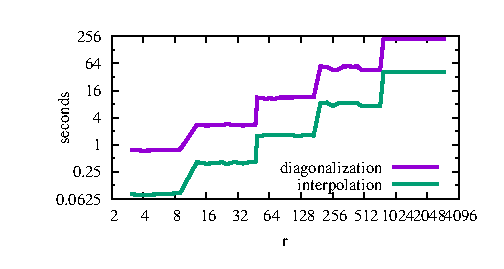
\includegraphics[scale=1]{benchmarks/graphe-101.eps} 


\begin{figure}
\includegraphics[scale=0.8]{benchmarks/graphe-101bis.pdf} 
%\resizebox{\columnwidth}{!}{\input{graphe-101}}
\caption{\label{fig:exp:uni} Comparaison entre la phase d'initialisation et la phase d'interpolation pour une courbe définie sur $\mathbb{F}_{101}$ pour $r$ croissant. La courbe est en échelle logarithmique.}
\end{figure}


On a donc regroupé dans la figure~\ref{fig:exp:uni} les deux premières parties
qui sont en fait du précalcul avec notamment le calcul de bases horiontales et 
comparé cela avec la troisième partie qui représente l'interpolation. On voit 
donc la linéarité en $r$ des temps de calcul. 
Le comportement en escalier observé est tout à fait normal car pour toutes les 
isogénies de degré 
$\frac{\ell^{2k-2}(\ell+1)}{4} \leqslant r \leqslant \frac{\ell^{2k}(\ell+1)}{4}$ 
on a besoin de travailler avec la même taille de $\ell^{k}$ torsion, ainsi pour 
différents $r$ dans cet intervalle on aura les polynômes $A_{a,b}$ et $T$ de 
même degré ce qui fait que la complexité et le temp de calcul sont les mêmes. 
Ceci est une raison 
suffisante pour motiver la recherche du plus petit nombre $\ell$ de Elkies car
alors on aura des paliers plus petits pour l'algorithme. Il pourrait toutefois 
s'avérer que pour un autre nombre de Elkies $\ell'$ plus grand que $\ell$, $r$ 
se trouve à la fin du palier $\frac{\ell'^{2k-2}(\ell+1)}{4} \leqslant r 
\leqslant \frac{\ell'^{2k}(\ell+1)}{4}$, ainsi il serait plus utile de 
travailler avec $\ell'$ plutôt que $\ell$.

Comme l'étape d'interpolation va être répétée $O(r \ell)$ fois et domine la 
complexité de l'algorithme~\ref{alg:cou:ell-adique} alors on compare le temps 
de calcul obtenu pour une étape d'interpolation pour différentes tailles de 
corps fini.
On présente donc une première série de tests qui a été réalisé sur des 
courbes qui ont toutes leur $\beta=h=2$, ainsi notre 
algorithme~\ref{alg:cou:ell-adique} a travaillé avec la $2^3$ torsion jusqu'à la 
$2^8$ torsion sur des courbes elliptiques définies sur corps finis premiers 
allant d'une taille de $7$ bits à $252$ bits. Le volcan de $2$-iogénies de 
gauche de la figure~\ref{fig:ex:niv:ext} est celui sur lequel se trouve la 
courbe définie sur $\mathbb{F}_{101}$ ayant servi aux calculs montrés dans la 
figure~\ref{fig:exp:dif}.

\begin{figure}
\begin{center}
%\include{benchmarks/graphe-101-149-269}
\includegraphics[scale=0.8]{benchmarks/graphe-101-2^18bis.pdf} 
%\include{graphe-101-149-269}
\caption{\label{fig:exp:dif} Comparaison d'une phase d'interpolation pour $r$ croissant pour différentes courbes définies sur les corps finis $\mathbb{F}_{101}$, $\mathbb{F}_{2^{18}+93 }$, $\mathbb{F}_{2^{30}+669}$, $\mathbb{F}_{2^{62}+189}$ et $\mathbb{F}_{2^{252}+421}$. La courbe est en échelle logarithmique.}
\end{center}
\end{figure}

On observe sur la figure~\ref{fig:exp:dif} que la dépendance en $q$ est plus 
grande que ce à quoi on aurait pu s'attendre d'après la borne théorique, cela 
doit être dû à des détails d'implantation bas-niveau que SageMath ne permet pas
de maîtriser.

\begin{figure}
%\input{graphe-521}
\includegraphics[scale=0.8]{benchmarks/graphe-521bis.pdf} 
\caption{\label{fig:exp:niv} Phase d'interpolation pour $r$ croissant pour différentes courbes définies sur les corps finis $\mathbb{F}_{521}$ et $\mathbb{F}_{1033}$. La courbe est en échelle logarithmique.}
\end{figure}

La deuxième série de tests montrés sur la figure~\ref{fig:exp:niv} a été réalisé
sur des courbes qui ont toutes leur $\beta=h=3$ définies sur des corps finis de
taille $p$ de $9$ bits, notre algorithme~\ref{alg:cou:ell-adique} a donc utilisé de la 
$2^4$ torsion jusqu'à $2^7$ torsion des courbes elliptiques. On voit ici que comme on a 
$\beta=h=3$ alors contrairement aux précédents tests il n'y a pas de palier où l'on travaille avec la 
$\ell^{3}$ torsion mais directement avec la $\ell^4$ torsion, car il est 
nécessaire d'avoir $k$ strictement supérieur à $h$.

Le détail des timings pour les 
différentes parties est disponible sur le projet github: 
\url{https://github.com/Hugounenq-Cyril/Two_curves_on_a_volcano}. 

\section{Cas Atkin}
\label{sec:Atk:Con}
On justifie tout d'abord l'intérêt de l'étude que l'on a fait de la forme de 
la matrice du Frobenius avec un vecteur de la base fixée par rapport à un 
algorithme de Couveignes~\cite{Couveignes96} modifié pour travailler avec la
$\ell$-torsion. Cette section utilise les résultats de la 
sous-section~\ref{subs:atk:dir}.

On énonce donc un résultat qui est une transposition de la 
proposition~\ref{pro:par:iso} qui s'appliquait au cas Elkies.

\begin{prop}\label{pro:par:iso:atk}
Soit~$\phi: E \rightarrow E'$ une isogénie de degré~$r$ premier avec~$\ell$ un 
nombre premier de Atkin.
\begin{enumerate}
\item les courbes~$E$,~$E'$ ont la même profondeur dans leur volcan des
 $\ell$-isogénies,
\item\label{pro:par:fun:atk} pour tout point~$P \in E[\ell^k]$,
les isogénies de noyau $\langle P \rangle$ et~$\langle \phi(P) \rangle$ sont de
même type (ascendantes, descendantes, ou horizontales de même direction),
\item\label{pro:par:asc:atk} si $P \in E[\ell]$ et $P' \in E'[\ell]$ sont tous 
les deux des points générateurs d'isogénies ascendantes alors $E/\langle P 
\rangle$ et~$E'/\langle P' \rangle$ sont encore $r$-isogènes.
\end{enumerate}
\end{prop}

\begin{proof}
La preuve est exactement la même que celle de la proposition~\ref{pro:par:iso}
toutefois ici on fait référence à la proposition~\ref{pro:mat:fro:atk} pour la
preuve.
\end{proof}

Voyons maintenant un résultat qui est une conséquence de la 
proposition~\ref{pro:atk:equi} et qui étudie donc l'invariance des groupes 
de point de $E[\ell^{\infty}]$ déterminé par l'action du Frobenius 
par rapport aux actions de $r$-isogénies rationnelles avec $r$ premier avec 
$\ell$.

\begin{cor}\label{cor:atk:ess}
Soit $\phi:E \rightarrow E'$ une $r$-isogénie avec $r \wedge \ell=1$ et $E$ et 
$E'$ deux courbes elliptiques, 
soient $P \in E$ et $P' \in E'$ deux points d'ordre $\ell^k$ avec $k>h$ tels 
que $P'=\phi(P)$ alors pour deux base $(P,Q),(P',Q')$ de $E[\ell^k]$ et 
$E'[\ell^k]$ telles que $\pi(P,Q)=\pi(P',Q')$ on a $[\ell^h]Q'=[\ell^h]\phi(Q)$. 
\end{cor}

\begin{proof}
Comme le Frobenius commute avec $\phi$ alors on a $\pi(P,Q)=\pi(\phi(P),\phi(Q))$
or comme $P'=\phi(P)$ pour $Q'$ tel que $\pi(P,Q)=\pi(P',Q')$ on a l'égalité 
$\pi(P',Q')=\pi(\phi(P),\phi(Q))$ et la proposition~\ref{pro:atk:equi} nous 
permet de conclure.
\end{proof}


On rappelle que l'on travaille avec deux courbes $r$-isogènes, avec $r \wedge 
\ell=1$ qui se situent sur un volcan de $\ell$-isogénies de hauteur $h$, dont 
le cratère est réduit à une courbe, car on se place dans le cas Atkin. On 
suppose de plus qu'un nombre $\ell$ de Atkin tel que $\ell^h<\sqrt{r}$ est déjà
connu (pour plus de détails voir la proposition~\ref{pro:bor:ell}). De plus on 
va dans un premier temps se restreindre au cas où les courbes avec lesquelles 
on travaille se situent sur le cratère d'un volcan de $\ell$-isogénies, on 
verra par la suite comment généraliser notre problème à des courbes non situées
sur le cratère.

Soient $E$, $E'$ deux courbes elliptiques de $j$-invariants $j$ et $j'$ reliées
par une $r$-isogénie $\phi$, $P \in E$ et $S' \in E'$ deux points d'ordre 
$\ell^{k}$, avec $k$  plus grand que $h$, tels que $\phi(P)=S'$. Pour deux 
bases $(P,Q),(S',R')$ de $E[\ell^k]$ et $E'[\ell^k]$ telles que $\pi(P,Q)=
\pi(S',R')$ on détermine de façon unique $\phi([\ell^h]Q)=[\ell^h]R'$ par le 
corollaire~\ref{cor:atk:ess}. On détermine alors le point 
$\phi(Q)$ en testant pour tout point $U'$ antécédent par $[\ell^h]$ de 
$[\ell^h]R'$ si la correspondance $(P,Q) \rightarrow (S',U')$ permet de définir
une $r$-isogénie. Ce test consiste comme dans le cas Elkies à calculer le 
polynôme d'interpolation $A_{S',U'}$ tel que 
\[
A_{R'}(x([u]P+[v]Q))=x([u]S'+[v]U') \quad \text{pour tout $[u]P+[v]Q$ d'ordre $\ell^k$}.
\]
Ensuite à l'aide du polynôme $A_{S',U'}$ on calcule la fraction rationnelle $F$ telle que:
\[
F=A_{S',U'} \bmod T
\]
avec $T$ le polynôme minimal qui s'annule sur tout point $[u]P +[v]Q$ 
d'ordre $\ell^k$. C'est la fraction rationnelle $F$ qui lorsque l'on a bien 
choisi $U'$ doit représenter l'action de la $r$-isogénie $\phi$, on cherche 
donc à calculer $F$ de degré $(r,r-1)$. Or une telle fraction rationnelle est 
déterminée par $2r$ coefficients on doit donc avoir le nombre d'abscisses de 
points d'ordre $\ell^k$: $\frac{\ell^{2k-2}(\ell+1)}{2}$ strictement plus grand
que $2r$ pour avoir suffisamment d'informations.

Comme la seule information que l'on ait sur l'image de $P$ par $\phi$ est que 
c'est un point d'ordre $\ell^k$, on propose donc de faire la procédure décrite 
dans le paragraphe précédent en testant toutes les valeurs possibles pour 
l'image de $P$ par $\phi$ c'est à dire tous les points d'ordre $\ell^k$ de 
$E'$.

%Dans la suite on se place dans le cas $\ell \neq 2$ par souci de simplicité. %Juste pour les tailles d'extensions de corps
On énonce des résultats qui sont des conséquences de la 
proposition~\ref{pro:clas:fro:atk} et qui nous seront utiles lors de l'étape 
du calcul de polynôme d'interpolation utilisant les méthodes de la 
section~\ref{sec:interpolation}.

\begin{cor}
Soit $P$ un point d'ordre $\ell^{\beta+i}$ de la courbe elliptique $E$ située 
au niveau du cratère du volcan de $\ell$-isogénies telle que $E(\mathsf{F}_
{1})[\ell^{\infty}] \simeq \mathbb{Z}/ \ell^{\beta} \mathbb{Z} \times 
\mathbb{Z}/ \ell^{\beta}\mathbb{Z}$, alors la taille de l'orbite de $P$ selon 
l'action de $\mathsf{Gal}(\mathsf{F}_{i+1}:\mathsf{F}_{1})$ est 
$\ell^i$. 
\end{cor}

\begin{cor} \label{cor:atk:orb:rep}
Soit $E$ une courbe elliptique située au niveau du cratère du volcan de 
$\ell$-isogénies telle que $E(\mathsf{F}_1)[\ell^{\infty}] \simeq 
\mathbb{Z}/ \ell^{\beta} \mathbb{Z} \times \mathbb{Z}/ \ell^{\beta}\mathbb{Z}$,
alors il y a $\ell^{2\beta + i -2}(\ell+1)$ classes de conjugaison de points 
d'ordre $\ell^{\beta+i}$ selon l'action de $\mathsf{Gal}(
\mathsf{F}_{i+1}:\mathsf{F}_{1})$.
\end{cor}


On peut dès lors énoncer une version $\ell$-adique de l'algorithme de 
Couveignes dans le cas Atkin dans l'algorithme~\ref{alg:cou:atk}.
\begin{algorithm}
\caption{\label{alg:cou:atk} Algorithme de Couveignes $\ell$-adique dans le cas Atkin.}
\begin{algorithmic}[1]
\REQUIRE $E,E'$: deux courbes elliptiques $r$-isogènes ordinaires situées au niveau du cratère d'un volcan de $\ell$-isogénies avec cratère réduit à une courbe.
\ENSURE $\phi$ la $r$-isogénie qui relie $E$ à $E'$.
% \STATE Calcul $(P_1,Q_1)$, a basis of $E[\ell]$
\STATE Calcul du plus petit $k$ tel que $\ell^{2k-2}(\ell+1)>4r$;
\STATE \label{alg:cou:atk:bas} 
Calcul de $(P,Q),(P',Q')$ bases de $E[\ell^k],E'[\ell^k]$;
\STATE \label{alg:cou:atk:frob:bas} Calcul de la matrice $\pi(P,Q)$;
\FOR{$S' \in E'$ d'ordre $\ell^k$} \label{alg:cou:atk:parc:poi}
\STATE \label{alg:cou:atk:matc:fro} Calcul de $R' \in E'$ tel que $\pi(S',R')=\pi(P,Q)$ à l'aide de l'algorithme~\ref{alg:atk:bas:mat}
\FOR{$U' \in E'$  tel que $[\ell^{h}]U'=[\ell^{h}]R'$} \label{alg:cou:atk:div:h}

\STATE Calcul des listes de représentants pour les orbites selon l'action du Frobenius $L$ et $L'_{U',R'}$ afin de respecter la correspondance induite par le choix de $U'$ et $R'$; \label{alg:cou:atk:rep}
\STATE \label{alg:cou:atk:int} Calcul des des polynômes $A_{S',U'}$ et $T$ par les méthodes décrites dans la section~\ref{sec:interpolation};
\STATE \label{alg:cou:atk:Cauchy} Calcul de la fraction rationnelle $F=A_{S',U'} \bmod T$ à l'aide d'une interpolation de Cauchy;
\IF{$\mathsf{Test}(F)$} \label{alg:cou:atk:test}
\RETURN $F$
\ENDIF
\ENDFOR
\ENDFOR 
\end{algorithmic}
\end{algorithm}

\begin{prop}
  \label{pro:atk:full-complexity}
  En supposant que l'on a $\ell^h<\sqrt{r}$, 
  l'algorithme~\ref{alg:cou:atk} calcule une $r$-isogénie 
  ${\phi:E \rightarrow E'}$ en un temps espéré de \[
  O(r \ell^2 \sqrt{r \ell}(\mathsf{M}(r\ell^4)\log(r)\log(\ell)+\mathsf{M}(\sqrt{r}\ell)\sqrt{r}\log(\ell)\log(\ell q))\]
auquel il faut ajouter un temps de pré-calcul de:
$O(r \mathsf{M}(\sqrt{r})\log(r)\log(\ell)+ \sqrt{r} \mathsf{M}(\sqrt{r})\log(\ell)\log(\ell q))$.
\end{prop}

\begin{proof}
On fait remarquer que la condition $\ell^h < \sqrt{r}$ signifie que l'on
a $k>h$, on va utiliser cette condition tout au long de la preuve.
Par définition de $k$ on a $\ell^{2k-1} \in O(r\ell^2)$.
Par la proposition~\ref{pro:clas:fro:atk}, il existe $\beta \leqslant h$ tel que
$E[\ell^k]$ est inclus dans $E(F_{k-\beta})$. On construit donc une
tour d'extensions $\ell$-adiques $\mathsf{F}_0\subset\cdots\subset 
\mathsf{F}_{k-\beta}$, et l'on effectue les précalculs nécessaires au 
théorème~\ref{thm:frob-ell} avec un coût de $O(\ell\mathsf{M}(\ell)\log(q))$.
\`A l'étape~\ref{alg:cou:atk:bas} le coût de calcul des bases de la 
$\ell^k$-torsion se fait à partir d'une base de la $\ell$-torsion puis on 
inverse la multiplication par $\ell$ l'aide de deux $\ell$-isogénies qui 
composent la multiplication par $\ell$. Par le lemme~\ref{lem:div:cou} le coût 
de calcul de $E[\ell]$ est de 
$O(\ell \mathsf{M}(\ell^2)\log(\ell)\log(\ell q))$ opérations sur 
$\mathbb{F}_q$, ensuite le coût de calcul de $\mathrm{divise}(\ell,P)$ pour 
$P \in E(F_n)$ est de $\mathsf{R}(n+1)$, ce coût est donc dominé par la 
dernière étape
$O(\mathsf{R}(k-\beta+1)+\ell \mathsf{M}(\ell^2)\log(\ell)\log(\ell q))$.
Par ~\cite[Chapter~14.5]{vzGJG03} on a $\mathsf{R}(n)=
O(\ell^n\mathsf{M}(\ell^{n+1})\log(\ell)\log(\ell q))$. 
L'étape~\ref{alg:cou:atk:bas} a donc un coût total de $O(\ell^k \mathsf{M}
(\ell^{k+1})\log(\ell)\log(\ell q))=O(\sqrt{r}\ell^{1,5}\mathsf{M}(\sqrt{r}\ell^{2,5})\log(\ell)\log(\ell q))$ 
dans le pire des cas où l'on aurait $\beta=1$.

De la même manière que l'algorithme~\ref{alg:atk:bas:mat} à l'étape~\ref{alg:cou:atk:frob:bas} on 
calcule itérativement l'action du Frobenius sur la $\ell^j$-torsion pour $j$ 
allant de $1$ à $k$, ainsi à l'étape $i \in [1;k]$ on a le coût du Frobenius
appliqué à un point de $\mathsf{F}_{i-\beta}$ lorsque $i>\beta$, $\mathsf{F}_1$
sinon qui est de $O(\ell^{\max(1,i-\beta)}\mathsf{M}(\ell))$ opérations sur 
$\mathbb{F}_q$ d'après le théorème~\ref{thm:frob-ell}. On effectue ensuite 
jusqu'à $2\ell^2$ additions de points définis sur $\mathsf{F}_{i-\beta}$ afin 
d'identifier l'action du Frobenius. Chaque étape a donc un coût de 
$O(\ell^2 \mathsf{M}(\ell^{\max(1,i-\beta)}))$,
le coût total de l'étape~\ref{alg:cou:atk:frob:bas} est donc de 
$O(\ell^2(\beta \mathsf{M}(\ell)+\mathsf{M}(\ell^{k-\beta+1})))=
O(\ell^2( \mathsf{M}(\ell)+\mathsf{M}(\sqrt{r}\ell^{1,5})))$ 
opérations sur $\mathbb{F}_q$ dans le pire des cas où $\beta=1$.

Le calcul de tous les points d'ordre $\ell^k$ à 
l'étape~\ref{alg:cou:atk:parc:poi} à partir d'une base de $E'[\ell^k]$ coûte 
$O(\mathsf{M}(\ell^k)\log(\ell^k)\ell^{2k})=
O(\mathsf{M}(\sqrt{r}\ell^{1,5})r\ell^3\log(r)\log(\ell))$ ce coût est considéré comme 
un pré-calcul.

L'étape~\ref{alg:cou:atk:matc:fro} a un coût de 
$O(\ell^4(\mathsf{M}(\ell^{k-\beta+1})+\beta\mathsf{M}(\ell)))$
opérations sur $\mathbb{F}_q$ d'après la proposition~\ref{pro:atk:comp:alg}.
Ce qui donne un coût de $O(\ell^4(\mathsf{M}(\sqrt{r}\ell^{1,5})+\mathsf{M}(\ell)))$.

L'étape~\ref{alg:cou:atk:div:h} calcule les antécédents d'un point d'ordre
$\ell^{k-h}$ par $[\ell^h]$ ainsi on utilise successivement la fonction 
$\mathrm{divise}(\ell,P)$ sur des points définis dans $\mathsf{F}_{k-h-\beta}$ à
$\mathsf{F}_{k-\beta}$, chaque itération de $\mathrm{divise}(\ell,P)$ a un coût
de $R(n+1)$ pour $P \in \mathsf{F}_n$ par le lemme~\ref{lem:div:cou}. Ainsi 
par ~\cite[Chapter~14.5]{vzGJG03} cette étape a un coût total de: 
$O(\mathsf{M}(\ell^{k-\beta +1})\ell^{k-\beta}\log(\ell)\log(\ell q)+\beta (\mathsf{M}(\ell^2)\ell\log(\ell)\log(\ell q)))$ 
ce qui donne dans le pire des cas
$O(\mathsf{M}(\sqrt{r}\ell^{1,5})\sqrt{r\ell}\log(\ell)\log(\ell q))$.

Par le corollaire~\ref{cor:atk:orb:rep} on a $\ell^{k+\beta-2}(\ell+1)/2$ 
représentants à calculer, chaque représentant étant 
calculé comme la multiplication scalaire d'un point d'ordre $\ell^k$ défini 
dans $\mathsf{F}_{k-\beta}$ par un coefficient dans 
$(\mathbb{Z}/\ell^k\mathbb{Z})^{\times}$ une telle multiplication a un coût
de $O(\log(\ell^k)\mathsf{M}(\ell^{k-\beta}))$. On a donc un coût total de 
$O(\mathsf{M}(\ell^{2k})\log(\ell^k))=O(\mathsf{M}(r\ell^3)\log(r))$ opérations sur 
$\mathbb{F}_q$ pour l'étape~\ref{alg:cou:atk:rep}.

Pour l'étape~\ref{alg:cou:atk:int} on utilise la 
proposition~\ref{prop:interpol} avec $t=\ell^{2k-2}(\ell+1)/2 \in O(r\ell^2)$ 
et le nombre de points d'interpolations $s=\ell^{k+\beta-2}(\ell+1)$, on 
calcule alors les polynômes $T$ et $A_{U',R'}$ avec un coût de 
$O(\mathsf{M}(r\ell^4)\log(r)\log(\ell))$. 

L'étape~\ref{alg:cou:atk:Cauchy} a une complexité de $O(r\log(r))$ d'après
\cite[Théorème 7.5]{algeff17}. Le coût du test de la fraction rationnelle est
dominé par les autres opérations (pour plus de détails le lecteur peut voir 
la preuve de la proposition~\ref{pro:full-complexity}).

Les étapes~\ref{alg:cou:atk:parc:poi} à ~\ref{alg:cou:atk:test} étant répétées 
$\ell^{k-h}$ fois cela a un coût de 
$O(\sqrt{r \ell}(\mathsf{M}(r\ell^4)\log(r)\log(\ell)+\mathsf{M}(\sqrt{r}\ell)\sqrt{r}\log(\ell)\log(\ell q))$ 
à $S'$ fixé.

Enfin l'étape~\ref{alg:cou:atk:frob:bas} et la boucle commençant à 
l'étape~\ref{alg:cou:atk:parc:poi} étant répétées $\ell^{2k-2}(\ell+1)/2 \in 
O(r\ell^2)$ fois cela donne une complexité de $O(r \ell^2 \sqrt{r \ell}(\mathsf{M}(r\ell^4)\log(r)\log(\ell)+\mathsf{M}(\sqrt{r}\ell)\sqrt{r}\log(\ell)\log(\ell q))$ à laquelle il faut ajouter les précalculs pour obtenir 
le résultat.
\end{proof}


Par la proposition~\ref{pro:par:iso:atk}, la profondeur de ~$E$ et $E'$ sous
leur cratère respectif est la même.  Par la
proposition~\ref{pro:par:iso:atk}~\ref{pro:par:asc:atk}, les
courbes sommets~$E_{s}$ et~$E'_{s}$ sont encore $r$-isogèness; on utilise
alors l'algorithme~\ref{alg:cou:atk} pour calculer une $r$-isogénie~$\psi_{s}$.  
Ensuite comme $\ell \wedge r =1$ alors $\psi = (\alpha ') \circ \psi_{s} \circ 
\alpha$ est bien définie et est la $r$-isogénie cherchée.
Le noyau de cette isogénie peut être calculé en $O(h\mathsf{\ell r}\log(\ell r))$
opérations en évaluant l'isogénie duale $\widehat{\alpha}$ sur le noyau de 
$\psi_s$ à l'aide d'une suite de résultants. \todo{Faire aussi cela}

Comme dit précédemment les résultats du lemmme~\ref{lem:cou:dec}, de la proposition~\ref{pro:bor:ell},
 et du corollaire~\ref{cor:atk:elk:dist} sont 
aussi valables dans le cas Atkin, on peut donc trouver un $\ell \in O(\log(q))$
nombre premier de Atkin tel que $\ell^h<\sqrt{r}$ et énoncer un résultat 
similaire à celui du théorème~\ref{thm:gen:elk:fin}, vu le peu d'intérêt d'un 
tel résultat on ne l'énoncera pas. 


%\begin{thm} \todo{resultat totaement inintéressant}
%Pour presque tous les nombres premiers $q$ et les courbes $E,E'$ définies sur 
%$\mathbb{F}_q$, il est possible de résoudre le problème du "Calcul de 
%l'isogénie explicite" avec l'algorithme~\ref{alg:cou:atk} en un temps espéré de
%\[
%O(r \ell^2 (\sqrt{r}(\mathsf{M}(r\ell^4)\log(r)\log(\ell)+\mathsf{M}(\sqrt{r}\ell)\sqrt{r}\log(\ell)\log(\ell q))))
%\]
%\end{thm}

\chapter{Variantes de l'algorithme de Couveignes $\ell$-adique dans le cas Elkies}
\label{cha:var:cou}
Dans les améliorations de l'algorithme de Couveignes que l'on a présentées 
seules celles concernant le cas Elkies ont un intérêt en terme de complexité. 
On va donc étudier des variantes à l'algorithme de Couveignes avec 
approche $\ell$ adique que dans le cas Elkies y compris lorsque celles-ci
auraient pu être appliquées à notre approche proposée pour le cas Atkin.
\section{Algorihme de Couveignes $\ell$-adique dans le cas Elkies avec un point horizontal}
\label{sec:var:cou:uni}
Comme proposé par François Morain on pourrait uniquement travailler avec un 
point horizontal au lieu de travailler avec une base horizontale.\todo{Dire ça ailleurs, dans les remerciements}

Au lieu de travailler avec une base horizontale dans l'algorithme de Couveignes
$\ell$-adique on pourrait tout aussi bien travailler avec une base horizontale.
Dés lors on devrait fixer $k$ tel que le nombre d'abscisses de points d'ordre 
$\ell^k$ engendrés par un point d'ordre $\ell^k$: $\frac{\ell^{k-1}}{2}$ soit 
strictement plus grand que $2r$.

Pour le calcul du point horizontal d'ordre $\ell^k$ on est tout de même obligé 
de calculer une base diagonale de la $\ell^{h+1}$-torsion et donc de 
travailler dans l'élément $\mathsf{F}_{h+1-\beta}$ de la tour d'extensions 
$\ell$-adiques.

\begin{prop}
Soit $k$ tel que $\ell^{k-1} \in O(r\ell)$, alors pour $h<k$ le coût de calcul d'une 
base diagonale de la $\ell^{h+1}$ torsion à l'aide de 
l'algorithme~\ref{alg:ulti:fro} est de:
\[
O(r \ell^{2} \mathsf{M}(r\ell^{3})\log(\ell)\log(\ell q) )
\]
\end{prop}

\begin{proof}
On rappelle que l'on travaille avec la convention $\alpha \geqslant \beta$, 
avec $\alpha$ et $\beta$ définis comme dans la définition~\ref{def:alp:bet}.
Le coût de calcul de la base horizontale est par la proposition~\ref{pro:alg:ulti}:
$O(\mathsf{R}(h+1)+ \mathsf{R}(k-\beta)+\ell^2 \mathsf{M}(\ell^{h+1})+\ell \mathsf{M}(\ell^2)\log(\ell)\log(\ell q))$. 
En bornant $h$ par $k$ on a $\ell^h \in O(r\ell)$ ce qui en utilisant cette
borne et le coût de $\mathsf{R}(i)$ donné par~\cite[chapter 14.5]{vzGJG03} nous 
donne une complexité de :
$O(r \ell^{2} \mathsf{M}(r\ell^{3})\log(\ell)\log(\ell q) )$.
\end{proof}
On observe donc que dans ce cas-là on a un coût quadratique en $r$ pour le 
calcul d'une base diagonale de la $\ell^{h+1}$ alors que dans le cas de la 
proposition~\ref{pro:full-complexity} on montrait dans la preuve que le coût 
d'une telle opération était quasi-linéaire.

Ensuite on calcule un point horizontal d'ordre $\ell^k$ à l'aide de 
l'algorithme~\ref{alg:hor:poi}, on rappelle qu'ici comme on détermine un seul 
sous-groupe cyclique on choisit de travailler avec celui défini 
sur la plus petite extension $\ell$-adique: $\mathsf{F}_{k-\alpha}$ d'où le 
fait que l'on ait $\alpha$ ici et non $\beta$ (pour rappel $\alpha$ et $\beta$ 
ont été définis dans la definition~\ref{def:alp:bet}). Ce calcul a un coût de 
$O(\mathsf{R}(k-\alpha) + k\mathsf{R}(h-\alpha+1) + k\ell^2\mathsf{M}(\ell^{h-\alpha+1}))$
d'après la proposition~\ref{pro:alg:hor}, ce qui appliqué à notre cas donne 
une complexité de: $O(r \ell \mathsf{M}(r \ell^{2})\log(\ell)\log(\ell q) \log(r))$.

Pour le calcul du polynôme d'interpolation on utilise des méthodes 
similaires à celles de la section~\ref{sec:interpolation} mais plus proches de 
celles de \cite[§5]{DeFeo11} vu qu'ici on travaille uniquement avec un sous-groupe 
cyclique défini dans $\mathsf{F}_{k-\alpha}$. 
On a alors au plus $\frac{\ell^{k-1}}{\ell^{k-\alpha}}=\ell^{\alpha-1}$ représentants 
des orbites selon l'action du Frobenius à calculer dans $\mathsf{F}_{k-\alpha}$.
Le calcul de ces représentants a un coût de 
$O(\ell^{\alpha-1}\mathsf{M}(\ell^{k-\alpha})\log(\ell^k)) \subset O(\mathsf{M}(r\ell)\log(r)\log(\ell))$ opérations.

Ensuite on doit calculer le polynôme d'interpolation en appliquant le résultat
 de la proposition~\ref{prop:interpol} avec $t=\ell^{k-1} \in O(r \ell)$, $s=\ell^{\alpha-1}$, 
 $n=k-\alpha$ on obtient une complexité de 
 $O(\mathsf{M}(\ell^3r)\log(\ell)\log(r))$ qui est l'étape dominante dans les
 étapes \ref{alg:cou-ell:ord} à \ref{alg:cou-ell:Cauchy} de 
 l'algorithme~\ref{alg:cou:ell-adique}.

Ainsi pour le calcul de la $r$-isogénie on doit répéter l'étape d'interpolation 
$\ell^{k-1}$ fois ce qui nous donne un coût total de: 
$O(r \ell \mathsf{M}(\ell^3r)\log(\ell)\log(r))$ opérations sur $\mathbb{F}_q$.

L'algorithme décrit ici est retranscrit dans l'algorithme~\ref{alg:app:cou:var}
en appendice~\ref{cha:alg} afin de ne pas surcharger ce document car comme vu 
juste au-dessus il est très similaire à l'algorithme~\ref{alg:cou:ell-adique}.

\begin{prop}
Soit $\ell$ un nombre de Elkies tel que $\ell^h<r$ alors le coût moyen de la 
variante de l'algorithme de Couveignes $\ell$-adique avec détermination d'un 
seul point horizontal présenté dans l'algorithme~\ref{alg:app:cou:var} 
est de: 
%\[
%O(r \ell (\mathsf{M}(r\ell^2)\log(\ell)\log(\ell q) \log(r) + \mathsf{M}(\ell^3r)\log(\ell)\log(r) ))
%\]
\[
O(r \ell \log(\ell) ( \mathsf{M}(r \ell^3) (\log(r) + \ell \log(q)) + \mathsf{M}(r \ell^2) \log(\ell q) \log(r) ) )
\]
opérations sur $\mathbb{F}_q$.
\end{prop}

Le coût de cette variante de Couveignes $\ell$-adique dans le cas Elkies a donc
une complexité qui est un peu plus faible que le résultat obtenu à la 
proposition~\ref{pro:full-complexity} avec un facteur $\ell$ en moins dans le 
calcul du polynôme d'interpolation. Ce facteur en moins vient du fait que l'on
cherche $k$ tel que $\ell^{k-1} >4r$ au lieu de $\ell^{2k-2}(\ell+1)>4r$ dés 
lors on obtient une meilleure précision dans le cas de cette variante pour le 
choix de $k$ ce qui fait que le coût du calcul du polynôme d'interpolation est
moins élevé de ce facteur $\ell$. On pourrait alors penser que cette variante
est meilleure que l'algorithme~\ref{alg:cou:ell-adique}
cependant l'algorithme~\ref{alg:cou:ell-adique} travaille dans des extensions 
de corps plus petites.
De plus notre estimation du nombre d'abscisses de points différentes utilisées lors de
l'interpolation est toujours très pessimiste car nous pourrions nous contenter de
prendre un nombre d'abscisses plus grand que $4r$, tout en ayant que des orbites 
complètes pour le Frobenius. Dès lors nous ne travaillerions pas avec $O(r\ell^2)$ 
abscisses lors de l'étape d'interpolation. Cependant la taille des orbites est
comprise entre $\ell^{k-\beta}$ et $\ell^{k-\alpha}$ dans notre approche (voir 
chapitres~\ref{cha:alg:fin} et ~\ref{cha:act:fro}). On aurait pu travailler avec
des orbites de taille plus petites si nous avions travaillé uniquement avec
des courbes situées sur le cratère du volcan de $\ell$-isogénies, nous aurions 
pu utiliser des points d'ordre compris entre $\ell^{k}$ et $\ell^{k-h}$. Ceci 
nous aurait permis de travailler avec des orbites plus petites et donc 
d'approcher $4r$ avec plus de précision.


Une différence notable c'est que dans cette variante la complexité pour le 
calcul d'une base diagonale de la $\ell^{h+1}$ torsion est quadratique alors 
que dans l'algorithme~\ref{alg:cou:ell-adique} cette partie est seulement 
quasi-linéaire en $r$.  Ainsi l'algorithme~\ref{alg:cou:ell-adique} présente
l'avantage d'avoir une partie quasi-linéaire fixe et une partie variable (pour 
le calcul de l'interpolation) quasi-quadratiqe en $r$ avec un aléa qui varie 
dans $O(r\ell)$ d'où le fait que cette variante ne propose pas de grand 
avantage par rapport à l'algorithme~\ref{alg:cou:ell-adique}.

Cette variante de l'algorithme~\ref{alg:cou:ell-adique}  proposé dans le cas 
Elkies non transposable à l'algorithme~\ref{alg:cou:atk} proposé dans le cas 
Atkin souligne le fait que l'étude de l'action du Frobenius dans le cas Elkies 
nous permet de spécifier des sous-groupe cycliques invariants par l'action de 
$r$-isogénies (avec $r \wedge \ell = 1$) alors que dans le cas Atkin on ne peut
que déterminer un sous-groupe cyclique à partir de la connaissance d'un autre 
sous-groupe cyclique.


On pourrait penser à utiliser l'algorithme de Couveignes $\ell$-adique avec 
différents nombres de Elkies $\ell_1, \ell_2, \ell_3, \dots, \ell_{n}$, pour 
une isogénie de degré $r$ premier avec tous les $\ell_i$. On 
calcule alors des bases horizontales de la $\ell_i^{k_i}$ torsion, on peut 
travailler avec les deux ensembles de points:
\begin{itemize}
\item $\cup_{i=1}^n \mathbb{Z}/\ell_i^{k_i} \mathbb{Z} \times \mathbb{Z}/\ell_i^{k_i} \mathbb{Z}$, 
\item $\prod_{i=1}^n \mathbb{Z}/\ell_i^{k_i} \mathbb{Z} \times \mathbb{Z}/\ell_i^{k_i} \mathbb{Z} $.
\end{itemize}
On va détailler chacune de ces approches dans les deux sous-sections qui suivent.

\section{Algorithme de Couveignes $\ell$-adique avec différents nombres de Elkies}
La première approche est de considérer l'ensemble de points $S$ isomorphe à: 
$\cup_{i=1}^n \mathbb{Z}/\ell_i^{k_i} \mathbb{Z} \times \mathbb{Z}/\ell_i^{k_i} \mathbb{Z} $,
avec les $\ell_i$ tous des nombres premiers de Elkies, dés lors il faut fixer comme 
condition  $\sum_{i=1}^n\ell_i^{2k_{i}-2}(\ell_i+1)>4r$
afin que le polynôme d'interpolation que l'on cherche à construire puisse 
définir la fraction rationnelle $F$ candidate pour représenter la $r$-isogénie 
$\phi$ que l'on veut calculer. 
L'avantage de cette approche est que bien que l'on soit obligé de travailler
sur différentes tours d'extensions $\ell$-adiques, on a pas besoin de 
travailler avec des compositum de tours d'extensions $\ell$-adiques.

Détaillons comment on procède, la méthode est restranscrite dans 
l'algorithme~\ref{alg:cou:mult-adique:short}.%, 
%l'algorithme~\ref{alg:cou:mult-adique} détaillant un peu plus 
%l'algorithme~\ref{alg:cou:mult-adique:short} est disponible en annexe.

\begin{algorithm}
\caption{\label{alg:cou:mult-adique:short} Algorithme de Couveignes $\ell$-adique avec différents nombres de Elkies}
\begin{algorithmic}[1]
\REQUIRE $E,E'$: deux courbes elliptiques $r$-isogènes ordinaires situées au niveau $h_i-e_i$ d'un volcan de $\ell_i$-isogénies avec cratère cyclique.
\ENSURE $\phi$ la $r$-isogénie qui relie $E$ à $E'$.
% \STATE Calcul $(P_1,Q_1)$, a basis of $E[\ell]$
\STATE Calcul des $k_i$ tel que $\sum_{i=1}^n\ell_{i}^{2k_{i}-2}(\ell_{i}+1)>4r$;
\FOR{$i=1$ à $n$}
\STATE \label{alg:mult-ell:bhor} Calcul de $(P_{\lambda,i},Q_{\mu,i}),
(P'_{\lambda,i},Q_{\mu,i}')$ bases (ascendantes) horizontales de 
$E[\ell_i^{k_i}],E'[\ell_i^{k_i}]$ à l'aide de l'algorithme~\ref{alg:ulti:fro} et de l'étape~\ref{alg:cou-ell:bhor} de l'algorithme~\ref{alg:cou:ell-adique};
\STATE \label{alg:mult-ell:rep} Calcul des liste de représentants $L_i,L_i'$ des orbites de points d'ordre $\ell_i^{k_i}$ sous l'action de $\pi$;
\ENDFOR
\FOR{$M \in \mathsf{diag}(a,b)$  avec $a,b \in \left( \mathbb{Z}/\prod_{i=1}^n\ell_i^{k_i}\mathbb{Z} \right)^{\times}$}
\FOR{$M_i \in \mathsf{diag}(a_i,b_i)$  avec $a=a_i \bmod \ell_i^{k_i},b=b_i \bmod \ell_i^{k_i}$}
\STATE \label{alg:mult-ell:ord} Actualisation de la liste des représentants $L_i'$ en $L'_{a,b,i}$ afin de respecter la correspondance induite par le choix de $M_i$;
\STATE \label{alg:mult-ell:int} Calcul des des polynômes $A_{a,b,i}$ et $T_i$ par les méthodes décrites dans la section~\ref{sec:interpolation};
\ENDFOR
\STATE Calcul des polynômes $A_{a,b}$ et $T$ à l'aide d'un théorème des restes chinois appliqué sur tous les $A_{a,b,i}$ et $T_i$;
\STATE \label{alg:mult-ell:Cauchy} Calcul de la fraction rationnelle $F=A_{a,b} \bmod T$ à l'aide d'une interpolation de Cauchy;
\IF{$\mathsf{Test}(F)$}
\RETURN $F$
\ENDIF
\ENDFOR 
\end{algorithmic}
\end{algorithm}

Les étapes \ref{alg:mult-ell:bhor} à \ref{alg:mult-ell:rep} de 
l'algorithme~\ref{alg:cou:mult-adique:short} qui calculent une base (ascendante) 
horizontale et des représentants des orbites de points (ascendants) 
horizontaux d'ordre $\ell_i^{k_i}$ sous l'action du Frobenius sont faites en 
parallèle sur chacune des tours d'extension $\ell_i$-adiques, les méthodes 
utilisées sont les mêmes que celles dans l'algorithme~\ref{alg:cou:ell-adique}.
Par les propositions~\ref{pro:par:iso} et ~\ref{pro:par:hor:par} on sait
 que pour tout $i$ l'action de $\phi$ sur une base
$(P_{\lambda,i},Q_{\mu,i})$ (ascendante) horizontale de $E[\ell_i^{k_i}]$ 
peut être représentée de la façon suivante:
$
\left(\begin{smallmatrix}
P'_{\lambda,i} \\
Q'_{\mu,i} 
\end{smallmatrix} \right)= \left(\begin{smallmatrix}
a_i & 0 \\
0 & b_i\end{smallmatrix} \right)
\left(\begin{smallmatrix}
P_{\lambda,i} \\
Q_{\mu,i} \end{smallmatrix} \right)$
avec $ a_i,b_i \in \left( \mathbb{Z}/\ell_i^{k_i}\mathbb{Z} \right)^{\times}$ et 
$(P'_{\lambda,i},Q'_{\mu,i})$
base (ascendante) horizontale de $E'[\ell_i^{k_i}]$.

On définit à l'aide du théorème des restes chinois deux coefficients $a,b \in 
\left( \mathbb{Z}/\prod_{i=1}^n\ell_i^{k_i} \mathbb{Z} \right)^{\times}$ tels que 
$a=a_i \bmod \ell_i^{k_i}$ et $b=b_i \bmod \ell_i^{k_i}$ pour $i\in [1,n]$.
On calcule ensuite pour chaque couple de coefficients 
$(a,b) \in (\mathbb{Z}/\prod_{i=1}^n\ell_i^{k_i}\mathbb{Z})^{\times}$ à l'aide des 
méthodes de la section~\ref{sec:interpolation} appliquées
à chacune des tours d'extensions $\ell_i$-adiques les polynômes 
d'interpolation $A_{a,b,i}$ et $T_i$ définis dans $\mathbb{F}_q$.
 On applique alors le théorème des restes chinois à ces polynômes pour obtenir 
 les polynômes $A_{a,b},T \in \mathbb{F}_q[x]$ tels que:
 \[
A_{a,b}=A_{a,b,i} \bmod T_i \text{ pour tout } i \in [1,n] \text{ et } \quad T=\prod_{i=1}^nT_i 
 \]
On fait le calcul de la fraction rationnelle $F=A_{a,b} \bmod T$ à l'aide d'une
interpolation de Cauchy. On teste si celle-ci est bien une $r$-isogénie,
si cela n'est pas le cas alors on recommence avec d'autres coeffcients $a,b \in 
(\mathbb{Z}/\prod_{i=1}^n\ell_i^{k_i} \mathbb{Z})^{\times}$.
%\newline

\paragraph{Analyse du coût}
{Une telle approche a forcément des coûts de pré-calcul (pour le calcul des bases 
horizontales et des représentants) plus faibles que notre approche dans 
l'algorithme~\ref{alg:cou:ell-adique}. De même dans la boucle que l'on effectue
 pour chaque choix de coefficients $a,b \in (\mathbb{Z}/\prod_{i=1}^n\ell_i^{k_i} \mathbb{Z})^{\times}$
le calcul des polynômes $A_{a,b,i}$ et $T_i$ définis dans $\mathbb{F}_q$ est 
inférieur au calcul de $A_{a,b}$ et $T$ à l'étape~\ref{alg:cou-ell:int} de 
l'algorithme~\ref{alg:cou:ell-adique} cependant le coût de calcul de 
l'interpolation de Cauchy  est de $O(\mathsf{M}(r)\log(r))$ par
 \cite[Théorème 7.5]{algeff17}. Sachant que l'on doit répéter en moyenne cette 
boucle pour tous les $a,b$ possibles appartenant à $(\mathbb{Z}/\prod_{i=1}^n\ell_i^{k_i} \mathbb{Z})^{\times}$
 le coût d'un tel algorithme est minoré par $\Omega(\prod_{i=1}^n\ell_i^{2k_i-2}
 \mathsf{M}(r)\log(r))$ et donc en particulier par $\Omega(r\mathsf{M}(r)
 \log(r))$. 

Une telle approche serait bien évidemment meilleure que 
l'algorithme~\ref{alg:cou:ell-adique} si l'on avait un moyen de préciser si un 
polynôme $A_{a,b,i_0}$ était correct sans connaître la valeur des autres 
$A_{a,b,i}$ dans un cas comme celui-ci on aurait à tester 
$\sum_{i=1}^n \ell_i^{2k_i-2} \in \Theta(r)$ choix possibles pour le polynôme 
d'interpolation, comme dans l'algorithme~\ref{alg:cou:ell-adique}.

Le principal inconvénient de cette approche 
c'est que l'on fixe comme condition sur les $k_i: \sum_{i=1}^n\ell_i^{2k_{i}-2}(\ell_i+1)>4r$
à cause du théorème des restes chinois à appliquer sur tous les $A_{a,b,i}$. 
On voudrait dés lors travailler avec des $k_i$ sur lesquels on aurait comme 
condition nécessaire: $\prod_{i=1}^n\ell_i^{2k_{i}-2}(\ell_i+1)>4r$
c'est ce que l'on va aborder dans la seconde approche avec des points 
(ascendants) horizontaux d'ordre composé $\prod_{i=1}^n \ell_i^{k_i}$.}

\section{Algorithme de Couveignes $\ell$-adique généralisé avec un nombre composé de Elkies}
Dans cette approche on veut travailler avec des points d'ordre 
$\prod_{i=1}^{n} \ell_i^{k_i}$ qui arrivent à porter l'information donnée par 
les  bases (ascendantes) horizontales $(P_{\lambda_i},Q_{\mu_i})$ de 
$E[\ell_i^{k_i}]$ avec $\ell_i$ un nombre premier de Elkies, pour faire cela on
a besoin de définir quelques notions. On va supposer sans perte de généralités 
que les $k_i$ pour $i \in [1,n]$ sont fixés tels que l'on ait $\prod_{i=1}^{n} 
\ell_i^{2k_i-2}(\ell_i+1)>4r$.
\label{sec:cou:con}
\subsection{Théorème des Restes Chinois et son application à l'algorithme de Couveignes $\ell$-adique}
\label{sub:TRCE:cou}


\begin{nota}
Introduisons la notation suivante afin d'alléger l'écriture par la suite: 
$\upsilon_n=\prod_{i=1}^n \ell_i^{k_i}$, 
$\vartheta_i=\frac{\upsilon_n}{\ell_i^{k_i}}$.
\end{nota}

\'Enonçons une généralisation du thèorème des restes chinois pour une courbe 
elliptique à $n$ nombres premiers distincts.

\paragraph{Théorème des Restes Chinois sur une courbe Elliptique $E$}
Soient $\ell_1, \dots, \ell_n$ $n$ nombres premiers distincts, les points $P_1 \in E[\ell_1^{k_1}], \dots, P_n \in E[\ell_n^{k_n}]$, alors le Théorème des Restes Chinois revient à déterminer un point $P \in E[\upsilon_n]$ tel que $[\vartheta_{i_0}] P=P_{i_0}$ pour $i_0 \in [1,n]$.

%\overset{n}{\underset{i \neq i_0}{\underset{i = 0}{\prod}}}\ell_i^{k_i}
On présente tout d'abord en appendice~\ref{cha:alg} l'algoritme~\ref{alg:TRC:init:gen} qui 
pour un point $P_{i}$ d'ordre $\ell_{i}^{k_{i}}$ calcule un point $P$ d'ordre 
$\upsilon_n$ tel que $[\vartheta_{i}]P=P_{i}$ et $[\ell_{i}^{k_{i}}]P$ pour 
$i \in [1,n]$. \`A l'aide de l'algorithme~\ref{alg:TRC:init:gen} on peut résoudre le 
Théorème des Restes Chinois comme montré dans l'algorithme~\ref{alg:TRC} lui aussi en appendice~\ref{cha:alg}

Cette approche du Théorème des Restes Chinois a été motivée pour l'appliquer à 
des points (ascendants) horizontaux d'ordre $\ell_i^{k_i}$, la proposition 
suivante montre que cette utilisation du théorème des restes chinois fait sens 
dans le contexte de l'algorithme de Couveignes.

\begin{prop}
\label{pro:par:TRC}
Soient $\ell_1, \ell_2$ deux nombres premiers distincts de Elkies, 
$P_1 \in E[\ell_1^{k_1}]$ un point horizontal d'ordre 
$\ell_1^{k_1}$ et de direction $\lambda_1$, $P_2 \in E[\ell_2^{k_2}]$ un point 
horizontal d'ordre $\ell_2^{k_2}$ et de direction $\lambda_2$. Soit $P \in 
E[\mathbb{Z}/\ell_1^{k_1}\ell_2^{k_2}\mathbb{Z}]$ un point d'ordre 
$\ell_1^{k_1}\ell_2^{k_2}$ tel que $\ell_1^{k_1}P=P_2$ et $\ell_2^{k_2}P=P_1$.
Soit $\phi$ une isogénie de degré $r$ premier avec $\ell_1, \ell_2$ alors 
$\phi(P)$ est tel que
\begin{itemize}
\item $\ell_1^{k_1}\phi(P)$ est un point horizontal d'ordre 
$\ell_2^{k_2}$ et de direction $\lambda_2$,  
\item $\ell_2^{k_2}\phi(P)$ est un point horizontal d'ordre 
$\ell_1^{k_1}$ et de direction $\lambda_1$,
\end{itemize}
\end{prop}

\begin{proof}
Par un raisonnement similaire à la preuve de la proposition~\ref{pro:par:iso}, 
vu que $\phi$ est de degré $r$ premier avec $\ell_1$ et $\ell_2$ alors on a un 
isomorphisme de modules de Tate qui commute avec le Frobenius.
\end{proof}

\begin{cor} 
\label{cor:par:TRC}
La proposition~\ref{pro:par:TRC} se généralise à $n$ nombre premiers de Elkies 
distincts premiers avec $r$.
\end{cor}

\begin{nota}
Soient $\ell_1, \dots, \ell_n$ $n$ nombres premiers de Elkies distincts, $P$ un
 point d'ordre $\upsilon_n$ de $E$ construit à l'aide du 
 théorème des restes chinois (voir algorithme~\ref{alg:TRC}) tel que 
$[\vartheta_i]P=P_i$ avec $P_i$ des points (ascendants) horizontaux de 
direction $\lambda_i$ et profondeur $e_i$, alors 
on dit que $P$ est de direction $(\lambda_1, \dots, \lambda_n)$ et de 
profondeur $(e_1, \dots, e_n)$. 
\end{nota}

\begin{rem}
Une application du corollaire~\ref{cor:par:TRC} et de la notation 
précédente est que pour deux courbes elliptiques $E,E'$ $r$-isogènes avec $r$ 
premier avec les nombres de Elkies $\ell_1, \dots, \ell_n$ un point $P \in E$ 
d'ordre $\upsilon_n$, de direction $(\lambda_1, \dots, \lambda_n)$ et 
profondeur $(e_1, \dots, e_n)$ a pour image par $\phi$ un point $[a]P' \in E'$
avec $a \in (\mathbb{Z}/\upsilon_n \mathbb{Z})^{\times}$ et $P'$ un 
point d'ordre $\upsilon_n$, de direction $(\lambda_1, \dots, \lambda_n)$ et 
profondeur $(e_1, \dots, e_n)$.
\end{rem}


\subsection{Construction de compositums d'extensions $\ell_i$-adiques}
\label{sub:con:com}

Cette partie s'appuie sur la construction de compositum à partir d'une idée de
%originale de \cite{BrawleyCarlitz87} reprise dans
\cite{DeFeoDoliskaniSchost14}, cet article donne aussi le moyen de calculer à un coût quasi 
linéaire le changement de représentation d'éléments du compositum. On veut donc
construire un corps dans lequel on pourrait représenter des points d'ordre 
$\upsilon_n$ construits à l'aide de points d'ordre $\ell_i^{k_i}$ représentés 
dans des tours d'extensions $\ell_i$-adiques comme celles décrites dans le 
chapitre~\ref{cha:tour}. Afin de ne pas surcharger la lecture de ce 
document de nombreuses preuves étant l'adaptation de techniques présentées 
dans le chapitre~\ref{cha:tour} elles ne seront pas détaillées.

Soient $\ell_1, \dots, \ell_n$ $n$ nombres premiers distincts, 
on va supposer dans le reste de ce document que les différentes tours 
d'extensions $\ell_i$-adiques sont définies comme dans le 
chapitre~\ref{cha:tour} dont on note les éléments 
$\mathbb{F}_q \subset \mathsf{F}_{(i,1)} \subset \dots \subset  \mathsf{F}_{(i,j)}$ 
ont chacune des degrés $d_i=[\mathsf{F}_{(i,1)}:\mathbb{F}_q]$ qui lorsqu'ils 
ne sont pas égaux à $1$ doivent être premiers entre eux (cette dernière 
restriction sera justifiée plus tard dans le document).

On veut donc tout d'abord définir un compositum de tours d'extensions 
$\ell_i$-adiques, en particulier on veut calculer un compositum qui contient 
tous les éléments des tours d'extensions $\ell_i$-adiques suivant:
$\mathsf{F}_{(1,k_1)}, \dots \mathsf{F}_{(n,k_n)}$. On suppose de plus que les
$\ell_i$ sont ordonnés de telle sorte que pour tout $i \in [2,n]$ 
$\prod_{j=1}^{i-1}d_j\ell_j^{k_j} \geqslant d_i\ell_i^{k_i}$, cette restriction
sert juste à simplifier les calculs.

On introduit un objet nécesaire à la construction de compositum.
\begin{defi}
Soient $P$ un polynôme unitaire de degré $\deg(P)$ de racines $r_i$ pour 
$i \in [1,\deg(P)]$, $Q$ un polynôme unitaire de degré $\deg(Q)$ de racines 
$s_j$, tels que $P$ et $Q$ aient des racines distinctes et des degrés $\deg(P),
\deg(Q)$ premiers entre eux, alors on définit $R$ le \emph{produit composé} 
comme étant le polynôme de degré $\deg(P)\deg(Q)$ unitaire et de racines 
$r_is_j$ avec $i \in [1,\deg(P)], j \in [1,\deg(Q)]$. On note $R= P\odot Q$.  
\end{defi}
On peut alors montrer comment on construit un compositum à l'aide de la 
proposition suivante: 
\begin{prop}
\label{pro:init:com}
Soient $\ell_1$ un nombre premier, $P$, $Q$ deux 
polynômes unitaires irréductibles de degré $d_1\ell_1^{k_1}$ et $\deg(Q)$ 
premiers entre eux tels que $\mathbb{F}_q[x]/\langle P \rangle \cong 
\mathsf{F}_{(1,k_1)}$ (le $k_1$ ème élément de la tour d'extensions 
$\ell_1$-adique vu dans le chapitre \ref{cha:tour}), $\mathbb{F}_q[y]/\langle Q 
\rangle$ une extension degré $\deg(Q)$ de $\mathbb{F}_q$.
 Soit $R=P\odot Q$  le produit composé de $P$ et $Q$, alors 
 $\mathbb{F}_q[z]/\langle R \rangle$ est un corps fini de taille 
 $q^{d_1\ell_1^{k_1}\deg(Q)}$ et est isomorphe à $\mathbb{F}_q[x,y]/
 \langle P,Q \rangle$.
\end{prop}

\begin{proof}
Voir \cite[Theorem 2]{BrawleyCarlitz87}
\end{proof}


On peut alors définir les compositum dans notre cas particulier.
\begin{defi}
\label{def:con:com}
On note $\mathbb{K}_1$ le corps $\mathsf{F}_{(1,k_1)}$. Soit $i \in [1,n-1]$ 
supposons que $\mathbb{K}_{i}$ est défini, alors à 
l'aide de la proposition~\ref{pro:init:com} $\mathbb{K}_{i+1}$ est défini comme
le compositum de $\mathbb{K}_i$ et $\mathsf{F}_{(i+1,k_{i+1})}$.
\end{defi}
\begin{rem}
Dans la définition~\ref{def:con:com} le cas où l'on aurait $d_i=d_j$ avec $d_i 
\neq 1$ pour $i \neq j$ entraîne le fait que l'on a pas
les conditions pour appliquer la proposition~\ref{pro:init:com}. 
Cette condition est assez restrictive car comme vu dans le 
chapitre~\ref{cha:tour} on a $d_i | \ell_i-1$ ainsi il est possible que l'on
ait pour $d_i,d_j$ distincts $\mathrm{pgcd}(d_i,d_j) \neq 1$. Une 
solution pour contourner ce problème serait alors de construire le compositum à
partir d'une extension de $\mathbb{F}_q$.
\end{rem}


%\cite{Schost15} pour un contexte) \todo{surement plus du tout utile}
\begin{nota} Afin de simplifier les notations on va 
 noter $p_{i}=\prod_{j=1}^{i}d_j\ell_j^{k_j}$, en particulier $p_{i}$ est le 
 degré du compositum $\mathbb{K}_i$ comme extension de $\mathbb{F}_q$, par 
 ailleurs on pose $p_0=1$.
%$m_i = \overset{n}{\underset{j \neq i}{\underset{j = 0}{\prod \ell_j^{k_j}}}}$
\end{nota}

Le coût de la construction d'un tel compositum n'est pas étudié en détail afin 
de ne pas surcharger le document car ce coût là ne sera pas majeur pour 
une application dans l'algorithme de Couveignes. Le résultat à utiliser pour 
évaluer un tel coût est le \cite[Theorem 1]{BostanFlajoletSalvySchost06} avec 
bien évidemûment les cots de construction de tours d'extension $\ell$-adiques 
vus dans le chapitre~\ref{cha:tour}.


 Comme motivé dans la sous sous section précédente~\ref{sub:TRCE:cou} on
 calcule les points (ascendants) horizontaux sur les volcans des 
 $\ell_i$-isogénies à l'aide des méthodes vues dans la 
 section~\ref{sub:con:poi}, on doit alors ensuite les exprimer dans le
 compositum afin de les utiliser pour le Théorème des Restes Chinois dans 
 l'algorithme~\ref{alg:TRC}.
  
 Voyons à quel coût on peut exprimer un élément de $\mathsf{F}_{(i,k_i)}$ dans 
 $\mathbb{K}_n=\otimes_{i=1}^n\mathsf{F}_{(i,k_i)}$. On a donc 
 besoin du résultat suivant issu de \cite[Theorem 1]{DeFeoDoliskaniSchost14}
 \begin{prop}[De Feo, Doliskani, Schost]
 \label{pro:com:inj}
 Soient $i \in [2,n] $ $P,Q$ deux polynômes irréductibles unitaires de degrés 
 premiers entre eux $d_i\ell_i^{k_i}$ et $p_{i-1}$ avec
   $\mathbb{F}_q[x]/\langle P \rangle \cong \mathsf{F}_{(i,k_i)}$ et 
   $\mathbb{F}_q[y]/\langle Q \rangle \cong \mathbb{K}_{i-1}$. Alors le 
   plongement d'un élément de $\mathsf{F}_{(i,k_i)} $  dans $\mathbb{K}_{i}$ a un
   coût de 
   $O(d_i\ell_i^{k_i}\mathsf{M}(p_{i-1})+p_{i-1}\mathsf{M}(d_i\ell_i^{k_i}))$ 
   opérations sur $\mathbb{F}_q$. La descente d'un élémént de $\mathbb{K}_{i} $
   vers un élément de $\mathsf{F}_{(i,k_i)}$  a un coût identique. 
   De même le plongement d'un élément de $\mathbb{K}_{i-1}$ dans 
   $\mathbb{K}_{i}$ aini que la descente d'un élément de $\mathbb{K}_{i}$ dans 
   $\mathbb{K}_{i-1}$ ont le même coût.
 \end{prop}

 \begin{proof}
 Voir \cite{DeFeoDoliskaniSchost14}.
\end{proof}  

 On sera amené à multiplier des polynômes à coefficients dans un 
 compositum, ainsi on a besoin du résultat suivant.

 \begin{prop}
 \label{pro:mul:com}
 La multiplication et la division euclidienne de polynômes de degré au plus $d$
 à coefficients dans $\mathbb{K}_{n} \cong \mathbb{F}_q[x]/ \langle P \rangle$
 avec $P$ un polynôme irréductible de degré $p_n$ est de $O(\mathsf{M}(p_nd))$ 
 opérations sur $\mathbb{F}_q$.
 \end{prop} 
 
 \begin{proof}
 La preuve est la même que celle de la proposition~\ref{pro:mult:pol}.
 \end{proof}
 
 On sera aussi amené à trouvé une racine d'un polynôme de degré $d$ à 
 coefficients dans un compositum $\mathbb{K}_n$, d'où le résultat suivant:
 
Maintenant voyons un résultat qui nous permet de changer la 
représentation d'un élément de $\mathbb{K}_i$ afin de le représenter comme un 
élément de $\mathbb{K}_{i-1} \otimes \mathsf{F}_{(i,k_i)}$. 

\begin{prop}[De Feo, Doliskani, Schost]
\label{pro:iso:fie}
Soient $i \in [1,n]$, $P(x),Q(y)$ deux polynômes irréductibles unitaires de degrés 
$d_i\ell_i^{k},p_{i-1}$ premiers entre eux à coefficients dans $\mathbb{F}_q$
qui définissent $\mathbb{F}_q[x]/\langle P \rangle \cong \mathsf{F}_{(i,k)}$,
$\mathbb{F}_q[x]/\langle Q \rangle \cong \mathbb{K}_{i-1}$. Soit $R=P \odot 
Q$ le produit composé de $P$ et $Q$ alors l'application de l'isomorphisme:
\begin{equation*}
\begin{alignedat}{1}
\varrho : \mathbb{F}_q[x,y]/\langle P, Q \rangle & \rightarrow \mathbb{F}_q[z]/\langle R \rangle \\
xy & \mapsto z
\end{alignedat}
\end{equation*}
a un coût de:
\begin{enumerate}
\item $O((d_i\ell_i^{k})^2\mathsf{M}(p_{i-1}))$ opérations sur $\mathbb{F}_q$
 et l'application de l'inverse de $\varrho$ a un coût de 
 $O(\mathsf{M}(d_i\ell_i^{k}p_{i-1})p_{i-1}^{1/2}+\mathsf{M}(d_i\ell_i^{k})p_{i-1}^{(\omega+1)/2})$ 
opérations sur $\mathbb{F}_q$ lorsque 
$d_i\ell_i^{k} \leqslant p_{i-1}$,
\item $O(p_{i-1}^2\mathsf{M}(d_i\ell_i^{k}))$ opérations sur $\mathbb{F}_q$ 
et l'application de l'inverse de $\varrho$ a un coût de 
$O(\mathsf{M}(p_{i-1}d_i\ell_i^{k})(d_i\ell_i^{k})^{1/2}+\mathsf{M}(p_{i-1})(d_i\ell_i^{k})^{(\omega+1)/2})$ 
opérations sur $\mathbb{F}_q$ lorsque $d_i\ell_i^{k} \geqslant p_{i-1}$.
\end{enumerate}
\end{prop}

\begin{proof}
Voir \cite{DeFeoDoliskaniSchost14}.
\end{proof}

Ainsi on va pouvoir appliquer ce résultat pour calculer le coût du Frobenius 
avec une méhtode similaire à celle du théorème~\ref{thm:frob-ell}, cela sera 
abordé dans la prochaine sous-section.

\subsection{Coût total de l'algorithme de Couveignes $\ell_i$-adique avec le Théorème des Restes Chinois}


\label{sss:crt:cou}
On a vu dans la sous-section~\ref{sub:TRCE:cou} 
qu'un point construit à l'aide du théorème des restes chinois appliqué à des 
points $P_i,Q_i$ (ascendants) horizontaux de directions $\lambda_i,\mu_i$  
d'ordre $\ell_i^{k_i}$, avec $r, \ell_i$ tous premiers entre eux, 
était mis en correspondance avec un autre point de même direction.
Ainsi avec deux bases de points (ascendants) horizontaux $(P_{\lambda_1,
\dots, \lambda_n},Q_{\mu_1, \dots, \mu_n}),(P'_{\lambda_1, \dots, \lambda_n}
 , Q'_{\mu_1, \dots, \mu_n})$ de $E[\prod_{i=1}^n\ell_i^{k_i}]$ et 
 $E'[\prod_{i=1}^n\ell_i^{k_i}]$ l'action de la $r$-isogénie peut être 
 représentée de la façon suivante:  
 \begin{equation*}
\left(
\begin{matrix}
P'_{\lambda_1, \dots, \lambda_n} \\
Q'_{\mu_1, \dots, \mu_n}
\end{matrix}
\right)= \left(\begin{matrix}
a & 0 \\
0 & b
\end{matrix} \right)
\left(
\begin{matrix}
 P_{\lambda_1, \dots, \lambda_n} \\
 Q_{\mu_1, \dots,  \mu_n} 
\end{matrix}
\right)
\quad \text{avec} \quad a,b \in \left( \mathbb{Z}/\prod_{i=i}^n\ell_i^{k_i}\mathbb{Z} \right)^{\times}.
\end{equation*}

On a donc bien une correspondance entre les points définis à l'aide du Théorème
des Restes Chinois appliqué à des points (ascendants) horizontaux définis 
sur deux courbes elliptiques $r$-isogènes avec $r$ premier avec $\ell_1, \dots
, \ell_n$.
 
Dans le but d'appliquer les même méthodes que celles de la 
sous-section~\ref{ssec:cou:elk} on a besoin de déterminer des représentants 
d'orbites sous l'action de groupes de Galois sur des éléments de 
$\mathbb{K}_n=\otimes_{i=1}^{n}\mathsf{F}_{(i,k_i)}$ le
défini dans la sous-section~\ref{sub:con:com}.
\begin{prop}
\label{pro:rep:com}
Soit $P$ un point d'ordre $\upsilon_n$ de $E(\mathbb{K}_n)$ obtenu à l'aide 
du Théorème des Restes Chinois appliqué aux points $P_i$ de $E$ d'ordre 
$\ell_i^{k_i}$ tels que l'orbite générée par l'action de 
$\mathsf{Gal}(\mathsf{F}_{(i,k_i)}:\mathbb{F}_q)$ sur $P_i$ soit de taille
 maximale: $d_i\ell_i^{k_i}$.  Alors l'orbite de $P$ selon l'action de 
 $\mathsf{Gal}(\mathbb{K}_n:\mathbb{F}_q)$ est elle aussi de taille maximale:
 $p_n=\prod_{i=1}^nd_i\ell_i^{k_i}$.
\end{prop} 
La preuve n'est pas retranscite pour ne pas surcharger le document.

\begin{nota}
Soient $\ell_1, \dots \ell_n$ $n$ nombres premiers de Elkies, alors on note 
$\epsilon_i$ le nombre de représentants de points d'ordre $\ell_i^{k_i}$ sous 
l'action d'un générateur de $\mathsf{Gal}(\mathsf{F}_{(i,k_i)}:\mathbb{F}_q)$.
\end{nota}

On voit donc avec la proposition~\ref{pro:rep:com} que pour déterminer des 
représentants pour l'orbite selon l'action du groupe de Galois pour des points 
d'ordre $\upsilon_n$ il suffit de calculer à l'aide du théorème des 
restes chinois tous les points $P$ d'ordre $\upsilon_n$ 
tels que tous les choix possibles de représentants $P_i=[\vartheta_i]P$
par rapport à l'action de $\mathsf{Gal}(\mathsf{F}_{(i,k_i)}:\mathbb{F}_q)$
 aient été effectués. Ainsi le nombre de représentants est
 donc de $\prod_{i=1}^{n} \epsilon_i$. On calcule donc 
 tout d'abord les représentants d'ordre $\ell_i^{k_i}$ dans les tours 
 d'extensions $\ell_i$-adiques, puis on les exprime dans le compositum et enfin
 on applique $\prod_{i=1}^{n} \epsilon_i$ fois le Théorème des Restes Chinois. 
  
 On peut dès lors modifier l'algorithme~\ref{alg:cou:ell-adique} de telle sorte
 que l'on travaille avec deux couples de points d'ordre 
 $\prod_{i=1}^n\ell_i^{k_i}$ de même direction.
 
 On présente donc l'algorithme~\ref{alg:cou:TRC-adique} qui résulte de cette approche ainsi qu'une 
 estimation de son coût.
 
\begin{algorithm}
\caption{\label{alg:cou:TRC-adique} Algorithme de Couveignes avec nombre composé de Elkies.}
\begin{algorithmic}[1]
\REQUIRE $E,E'$: deux courbes elliptiques $r$-isogènes ordinaires situées au niveau $h_i-e_i$ d'un volcan de $\ell_i$-isogénies avec cratère cyclique pour $i$ allant de $1$ à $n$.
\ENSURE $\phi$ la $r$-isogénie qui relie $E$ à $E'$.
% \STATE Calcul $(P_1,Q_1)$, a basis of $E[\ell]$
\STATE Calcul des $k_i$ tels que $\prod_{i=1}^n\ell_{i}^{2k_{i}-2}(\ell_{i}+1)>4r$;
\FOR{$i=1$ à $n$}
\STATE \label{alg:cou:TRC-adique:bhor} Calcul de $(P_{\lambda,i},Q_{\mu,i}),
(P'_{\lambda,i},Q_{\mu,i}')$ bases (ascendantes) horizontales de 
$E[\ell_i^{k_i}],E'[\ell_i^{k_i}]$ à l'aide de l'algorithme~\ref{alg:ulti:fro} 
et de l'étape~\ref{alg:cou-ell:bhor} de l'algorithme~\ref{alg:cou:ell-adique};
\STATE \label{alg:cou:TRC_adique:rep:uni} Calcul des représentants des orbites de points d'ordre $\ell_i^{k_i}$ sous l'action de $\mathsf{Gal}(\mathsf{F}_{(i,k_i)}:\mathbb{F}_q)$;
\ENDFOR
\STATE \label{alg:cou:TRC-adique:TRC} Calcul de $(P,Q),(P',Q') \in E^2 \times E'^2$ d'ordres $ \mathbb{Z}/\prod_{i=1}^n \ell_i^{k_i}\mathbb{Z}$ tels que $P$ et $P'$ sont de direction $(\lambda_1, \dots, \lambda_n)$ et $Q$ et $Q'$ de direction $(\mu_1, \dots, \mu_n)$ à l'aide de l'algorithme~\ref{alg:TRC};
\STATE \label{alg:cou:TRC-adique:rep} Calcul des listes de représentants $L_i,L_i'$ des orbites de points d'ordre $\prod_{i=1}^n \ell_i^{k_i}$ sous l'action de $\mathsf{Gal}(\mathbb{K}_n:\mathbb{F}_q)$;
\FOR{$M \in \mathsf{diag}(a,b)$  avec $a,b \in \left( \mathbb{Z}/\prod_{i=1}^n\ell_i^{k_i}\mathbb{Z} \right)^{\times}$}
\STATE \label{alg:cou:TRC-adique:ord} Actualisation de la liste $L_i'$ en $L'_{a,b}$ afin de respecter la correspondance induite par le choix de $M$;
\STATE \label{alg:cou:TRC-adique:int} Calcul des des polynômes $A_{a,b}$ et $T$ par des méthodes similaires à celles décrites dans la section~\ref{sec:interpolation};
\STATE \label{alg:cou:TRC-adique:Cauchy} Calcul de la fraction rationnelle $F=A_{a,b} \bmod T$ à l'aide d'une interpolation de Cauchy;
\IF{$\mathsf{Test}(F)$} \label{alg:cou:TRC-adique:test}
\RETURN $F$
\ENDIF
\ENDFOR 
\end{algorithmic}
\end{algorithm}

Avant d'évaluer le coût de l'algorithme~\ref{alg:cou:TRC-adique}, qui comme on
a vu avec l'algorithme~\ref{alg:cou:ell-adique}, est dominé par le coût de 
l'interpolation (étape~\ref{alg:cou:TRC-adique:int}) on énonce le coût du
Frobenius (sans rentrer dans les détails) et on estime le calcul de polynômes 
d'interpolation. 

\begin{prop}
\label{pro:fro:com}
Soit $i \in [1,n]$, $P$ un polynôme irréductible de degré $d_i\ell_i^{m}$ avec 
$m \in [1,k_i]$ tel que $\mathsf{F}_{(i,m)}=\mathbb{F}_q[x]/\langle P \rangle$,
$Q$ un polynôme irréductible de degré $p_{i-1}=\prod_{j=1}^{i-1}d_j\ell_j^{k_j}$
tel que $\mathbb{K}_{i-1}=\mathbb{F}_q[y]/\langle Q \rangle$, $R=P \odot Q$ 
tel que  $\mathsf{K}=\mathbb{F}_q[z]/\langle R\rangle$, alors pour un 
élément $a$ du corps $\mathsf{K}$ le coût de calcul de $a$ à une puissance 
$q^{r p_{i-1}}$ est de 
$O(\mathsf{M}(d_i\ell_i^{m}p_{i-1})p_{i-1}^{1/2}+\mathsf{M}(d_i\ell_i^{m})p_{i-1}^{(\omega+1)/2})$ 
opérations dans $\mathbb{F}_q$ avec un 
précalcul qui a un coût booléen de $O(\log(p_{i})\log(\ell_i^{k_i}qd_i))$ et  
de $O( M(d_i) d_i\log(q))$ opérations sur $\mathbb{F}_q$.
\end{prop}

%On voit dans cette preuve que le coût de changement de représentation des 
%éléments de $\mathbb{K}_i$ vers une représentation de la forme 
%$\mathbb{K}_{i-1} \otimes \mathsf{F}_{(i,n_i)}$ est crucial dans le coût total
%du Frobenius. En effet si on compare ce résultat avec celui du
 
On obtient donc un résultat moins bon que celui du
théorème~\ref{thm:frob-ell}, or en adaptant les mêmes méthodes on aurait du 
avoir le coût de cette opération dominé par $O(d_i\ell_i^{k_i})\mathsf{M}(p_{i-1})$. 
Cependant ici, contrairement au cas du théorème~\ref{thm:frob-ell}, on doit prendre en 
compte le coût du changement de représentation qui domine la complexité. Ainsi 
il est crucial si l'on veut obtenir des résultats similaire à la 
section~\ref{sec:interpolation} d'avoir une construction de compositum permettant un 
changement de représentation à un coût linéaire.

Une adaptation des méthodes de calcul de polynôme d'interpolation décrites dans
la section~\ref{sec:interpolation} à ce contexte est faite pour le calcul de 
polynôme minimal $T=T^{(n)}$(en reprenant une notation similaire) d'éléments de 
$\mathbb{K}_n \setminus \mathbb{K}_{n-1}$.
Ainsi, comme dans la section~\ref{sec:interpolation}, 
pour le calcul d'un tel polynôme d'interpolation on est amené à 
multiplier des polynômes à coefficients dans $\mathbb{K}_{n-i-1} \otimes 
\mathsf{F}_{(n-i,k)}$ qui de par leur degré font que le coût d'une telle 
multiplication n'est que de $\tilde{O}_{p_n,q}(\mathsf{M}(p_n))$. Ce coût de 
$\tilde{O}_{p_n,q}(\mathsf{M}(p_n))$ en comparant 
avec les résultats du lemme~\ref{lemma:interpolation:minpoly} devrait être le 
coût dominant. Cependant par le coût de 
l'application du Frobenius aux polynômes $T^{(i)}_k$ de $O(\mathsf{M}
(p_n)p_{n-i-1}^{(\omega-1)/2})$, on majore le coût total du Frobenius par 
$O(n\mathsf{M}(p_n)p_{n-1}^{(\omega-1)/2}\max_i(\ell_{i}(k_{i}+1)))$. %or on doit appliquer le Frobenius 
%$\ell_{n-i}(k_{n-i}+1)$ fois et donc on majore ce coût.

De la même manière pour le calcul des polynômes d'interpolation $A$ tels 
$A(v)=w$ avec $v,w \in \mathbb{K}_n \setminus \mathbb{K}_{n-1}$, le coût est
encore une fois dominé par l'application du Frobenius et on majore le coût d'un
tel calcul par \[O(n\mathsf{M}(p_n \max_i(d_i\ell_i^{k_i}))
\max_i(\ell_i(k_i+1))p_{n-1}^{(\omega-1)/2}).\]

Ensuite pour $(v_1,w_1),\dots,(v_s,w_s)$ des paires d'éléments de $\mathbb{K}_n~\setminus~\mathbb{K}_{n-1}$, $t_j$ le degré des polynômes minimaux de $v_j$, on note  $t=\sum t_j$. 
On veut alors calculer les polynômes
  \begin{itemize}
  \item $T\in \mathbb{F}_q[x]$ de degré $t$ tel que $T(v_j)=0$ pour tout $j$,
    et
  \item $A\in \mathbb{F}_q[x]$ de degré inférieur à $t$ tel que $A(v_j)=w_j$ pour
    tout $j$.
  \end{itemize}
On utilise à nouveau la méthode de la section~\ref{sec:interpolation}, le 
calcul de $T$ à partir des $T_j$ a un même
coût que dans la proposition~\ref{prop:interpol} de $O(\mathsf{M}(t)\log(s))$. 
Cependant comme vu précédemment le coût de calcul des $A_j$ est de 
\[
O(n\mathsf{M}(t_j\max_i(d_i\ell_i^{k_i}))(p_{n-1})^{(\omega-1)/2}
\max_i(\ell_i(k_i+1)))
\]
on majore donc le coût total par
\[O(n\mathsf{M}(t\max_i(d_i
\ell_i^{k_i}))(p_{n-1})^{(\omega-1)/2}\max_i(\ell_i(k_i+1)))\]
par superlinéarité de 
$\mathsf{M}$.

On peut donc estimer le coût de cette version $\ell$-adique de l'algorithme de 
Couveignes à l'aide du coût dû à l'interpolation. 
L'interpolation étant répétée $O(r \prod_{i=1}^n\ell_i)$ en moyenne, on obtient
une estimation de 
\[ O(r (\prod_{i=1}^n\ell_i)n\mathsf{M}(r (\prod_{i=1}^n \ell_i^2)
\max_i(d_i\ell_i^{k_i}))(p_{n-1})^{(\omega-1)/2}\max_i(\ell_i (k_i +1)) ).\] 
Avec $p_n \in O(r(\prod_{i=1}^n\ell_i)^{3,5})$ on a une estimation 
de 
\[ 
O(r(\prod_{i=1}^n\ell_i)n\mathsf{M}(r (\prod_{i=1}^n \ell_i^{3,5})
\max_i(d_i\ell_i^{k_i}))(r (\prod_{i=1}^n \ell_i^{3,5}))^{(\omega-1)/4}
\max_i(\ell_i(k_i+1)) )
\]
sachant que la borne du calcul des $T_i$ et $A_i$ est large car on a majoré 
$\sum_{i=1}^np_{n-i}^{(\omega-1)/2}$ par $np_{n-1}^{(\omega-1)/2}$ d'où le 
$n$ en facteur et que de plus 
$\max_i(d_i\ell_i^{k_i})p_{n-1} \in \Omega(p_n)$. Ainsi on voit que par 
l'apport d'opérations de changement de représentations non-linéaires en la 
taille des compositum on ne peut avoir une complexité quadratique en $r$ pour
le calcul de l'isogénie montrant ainsi qu'une telle approche en l'état actuel
n'est pas intéressante. Cependant cette approche avait l'avantage de proposer
une meilleure estimation de $r$ par $\prod_{i=1}^n \ell_i^{k_i}$ et donc de 
réduire les coûts apportés par l'étape d'interpolation dûs au choix des
nombres premiers de Elkies.


 

\chapter*{Conclusion}
Nous avons donc vu dans ce manuscrit comment généraliser l'algorithme de 
Couveignes au cas $\ell$-adique. En particulier, nous avons 
vu que l'on était capable d'obtenir un algorithme qui résolve le problème de 
l'isogénie explicite avec une complexité quasi-quadratique en le degré de 
l'isogénie uniquement dans le cas Elkies, et un algorithme de complexité 
inférieure à cubique dans le cas Atkin. Cependant notre proposition 
d'algorithme $\ell$-adique de Couveignes dans le cas Atkin
a une complexité trop grande. Une amélioration de l'algorithme que nous proposons
dans le cas Atkin, avec la même méthode que pour le cas Elkies, nécessiterait 
de distinguer un sous-groupe cyclique de la $\ell^k$-torsion, ou de trouver un 
autre moyen pour distinguer des couples de points formant une base de 
$E[\ell^k]$. Nous avons 
réfléchi à travailler avec un groupe de points isomorphe à 
$\mathbb{Z}_{\ell^2}$ (l'unique extension quadratique non ramifiée de 
$\mathbb{Z}_{\ell}$), mais nous n'avons pas réussi à modéliser l'action du 
Frobenius sur un tel ensemble.
\todo{Je ne comprends pas ce que tu veux faire.}
Enfin, parmi les pistes proposées mais non 
satisfaisante dans le chapitre~\ref{cha:var:cou}, seule celle présentée dans la 
section~\ref{sec:cou:con} utilisant un nombre composé de Elkies 
pourrait aboutir, en supposant qu'on ait des meilleures représentations de composita 
permettant des changements de représentation de corps finis en un temps quasi-linéaire.

Nous donnons, pour conclure, quelques perspectives d'application des
résultats de cette thèse.

\paragraph{Calcul d'anneaux d'endomorphismes}
Les propositions~\ref{pro:mat:fro} et \ref{pro:mat:fro:atk} nous 
permettent de savoir exactement à quel niveau se trouve une courbe dans un 
volcan de $\ell_i$-isogénies. Ainsi en se plaçant dans le même contexte que 
\cite{BissonSutherland11},
\todo{Et de la thèse de Kohel, et de celle de Gaëtan, non?}
où l'on connaît déjà une factorisation de $d_{\pi}$, grâce à ces résultats
on connaîtrait la valuation $\ell_i$-adique du 
conducteur de la courbe par rapport à $\mathbb{Z}[\pi]$, et donc on pourrait
déterminer l'anneau des endomorphismes de la courbe. Cela pourrait avoir, par 
exemple, une application dans l'algorithme de Bröker \cite{Broker08} utilisé 
pour calculer un polynôme de Hilbert.
\todo{Je crois que la littérature sur le calcul de polynômes d'Hilberts est un peu plus
  vaste que ça. Il doit y avoir des papiers d'Andreas et de Drew, entre autres.}
En effet dans l'algorithme de Bröker, il 
est nécessaire de calculer une courbe avec un anneau d'endomorphismes 
spécifique à partir d'une courbe au hasard dont $\mathbb{Z}[\pi]$ est fixée. 
On pourrait alors à partir d'une telle courbe se servir des 
propositions~\ref{pro:mat:fro} ou \ref{pro:mat:fro:atk} afin de déterminer 
l'anneau des endomorphismes de la courbe.
Ensuite on pourrait se servir de la proposition~\ref{pro:tri:dir} ou du 
corollaire~\ref{cor:mon:atk} pour trouver une courbe dont 
l'anneau des endomorphismes correspond à celui que l'on cherche.
\todo{Peut-être deux mots pour dire pourquoi ce serait plus intéressant d'utiliser
  tes résultats, plutôt que la thèse de Kohel, ou Fouquet-Morain, ou Miret et al. etc.?}

\paragraph{Déplacement sur le cratère de volcans de $\ell$-isogénies et ses 
applications aux algorithmes de calcul de poylnômes de Hilbert et modulaire}
Des articles tels que \cite{Couveignes96isogenycycles}, \cite{Broker08}, 
\cite{Sutherland11a}, \cite{BLS12}, utilisent des marches sur le cratère 
cyclique d'un volcan de $\ell$-isogénies avec $\ell$ petit. Certains 
algorithmes (\cite{Couveignes96isogenycycles}) se limitent, à juste titre, au 
cas de volcans réduits à leur cratère, d'autres ne peuvent, et on va donc 
aborder l'éventuel impact de nos travaux sur ceux-ci.
Dans l'algorithme de Sutherland \cite{Sutherland11a} pour le calcul de polynômes
de Hilbert on est obligé, de par la taille du $\ell$-ème 
polynôme modulaire, de traiter les cas où le volcan n'est pas réduit à un
cratère cyclique. Dés lors il serait pertinent de voir l'apport de notre 
travail (proposition~\ref{pro:dia:hor}) dans ce contexte par rapport à 
l'algorithme utilisé par Sutherland, similaire aux travaux de 
\cite{FouquetMorain02} (voir sous-section~\ref{sub:alg:FM}) se servant
du $\ell$-ème polynôme modulaire, ainsi on pourrait rendre cet algorithme non
dépendant du (pré)calcul des polynômes modulaires.
Dans l'algorithme de Bröker, Lauter et Sutherland \cite{BLS12}, pour 
calculer le $\ell$-ème polynôme modulaire les auteurs se placent dans le cas
d'un volcan de $\ell_i$-isogénies de hauteur $1$,
pour lequel on a $E[\ell_i]\subset E(\mathbb{F}_p)$ pour les courbes situées
sur le cratère et pour lequel on a l'existence de points d'ordre $\ell_i^2$ 
définis sur $\mathbb{F}_p$ pour les courbes en bas du volcan.
\todo{C'est pas la même chose que dire Elkies, de hauteur 1 et régulier, ça?}
On pourrait à 
nouveau étudier, dans ce cas très spécifique, l'impact d'une méthode utilisant
la proposition~\ref{pro:dia:hor}.



%Dans les travaux similaire à \cite{BissonSutherland11} \todo{reformuler cela} pour le calcul 
%d'anneau d'endomorphisme tels que \cite{BLS12} pour le calcul de polynôme 
%modulaire ou le calcul de polynôme de Hilbert \cite{Broker08} \cite{Sutherland11a}
%sont utilisés des marches sur le
%volcan, et se placent par simplicité dans le cas où le volcan de 
%$\ell_i$-isogénies est réduit à un cratère cyclique. Ce cas se présentant 
%uniquement pour les nombres $\ell_i$ de Elkies ne divisant pas $d_{\pi}$, cette 
%approche est trés raisonnable. De plus comme dit dans \todo{trou} le calcul d'isogénies 
%n'est pas privilégié or c'est ce que l'on fait lors de nos déplacements dans
%la détermination de direction dans le volcan. Pour toutes ces raisons notre 
%détermination de directions dans le volcan de $\ell_i$-isogénies n'aura 
%vraisemblablement pas d'impact sur ces méthodes. Cependant comme dit dans \todo{trou}
%où l'on étudie les directions dans le volcan à l'aide d'action dans le groupe
%de classes d'idéaux, il serait intéressant de savoir transposer le résultat de 
%la proposition~\ref{pro:dia:hor} au groupe de classes d'idéaux pour avoir 
%éventuellement un résultat intéressant dans ce contexte.
\paragraph{Multiplication scalaire et points ascendants horizontaux}
On a aussi vu dans le chapitre~\ref{cha:tour}, en adaptant les méthodes de 
\cite{Doliskani-Schost15}, un moyen de faire un calcul 
rapide du Frobenius.
\todo{D'une courbe ou du corps?}
Il serait intéressant de voir si on ne peut pas se servir
de cela pour obtenir des résultats intéressants sur la multiplication scalaire.
Pour le moment tout ce que l'on est capable de faire c'est, à partir d'une 
décomposition d'un point $R$ d'ordre $\ell^k$ en deux points (ascendant) 
horizontaux $P_{\lambda}, Q_{\mu}$ décomposer la multiplication scalaire de 
$R=[a]P_{\lambda} + [b] Q_{\mu}$ par $c$ en le calcul de $[c]R=[c_{\lambda}] 
\pi^{\lfloor c/\lambda \rfloor}([a]P)+[c_{\mu}]\pi^{\lfloor c/\mu \rfloor}
([a]Q_{\mu})$  avec $c_{\lambda}=c \bmod \lambda$ et $c_{\mu}=c \bmod \mu$. 
L'intérêt d'une telle approche reste à étudier.
\todo{Tu veux faire un truc à la GLV? Cite.}

\paragraph{Crypto-système}
On pourrait utiliser, dans le cas Atkin, le résultat de la proposition ~\ref{pro:cla:fro:mat}
pour faire un crypto-système dans lequel le point $P$ fixé serait la clé maitre 
secrète partagée entre deux utilisateurs. Dés lors ces utilisateurs se 
communiqueraient la forme de matrices du Frobenius et déterminerait à l'aide de
$P$ le second point de la base qui serait alors une nouvelle clé partagée.
Ce crypto-système semble cependant un peu trop couteux pour être pratique.
\todo{BS. Enlève-moi ça!}

\paragraph{Couplage de points}
Le couplage de points n'a pas été abordé dans ce document mais seulement 
mentionné, certes dans \cite{Ionica-Joux10} il y a des résultats moins probants
sur la détermination de directions dans le volcan de $\ell$-isogénies. Il 
serait toutefois intéressant d'étudier si le couplage ne nous apporte pas un 
critère restrictif, pertinent du point de vue de la complexité, sur les images 
de points par la $r$-isogénie, et en particulier sur les points (ascendants) 
horizontaux.
\todo{Ce paragraphe irait mieux dans la discussion sur comment améliorer tes résultats,
  que tu fais avant ``Calcul d'anneaux d'endomorphismes''.
  Il ne s'agit pas d'une application de tes résultats.}

\paragraph{Calcul d'isogénies de degrés non connus}
Comme abordé dans la thèse de De Feo \cite[Section 8.9]{DeFeo10}, l'algorithme 
de Couveignes \cite{Couveignes96} pourrait être utilisé sans connaître le degré
de l'isogénie, donc nos algorithmes de Couveignes $\ell$-adique aussi. Nos 
algorithmes auront ainsi l'avantage de ne pas dépendre de la caractéristique du
corps sur lequel ils se trouvent.
\todo{C'est trivial. Mais si tu n'as pas plus d'idées de quoi faire avec ça,
  pas la peine d'en parler.}

De manière plus générale on pourrait étudier l'intérêt de l'algorithme de 
Couveignes $\ell$-adique dans la cryptanalyse de systèmes à base d'isogénies.
\todo{Trop spécifique. Si Couveignes donne quelque chose, pourquoi pas les autres
  algos de calcul d'isogénies? Certes, tu as envie de t'intéresser à la cryptanalyse
  de IBC, et c'est bien, mais ta thèse n'apporte pas grande chose de nouveau
  sur le sujet.}
 
\todo{Vérifier qu'il n'y a pas d'erreurs dans la bibliographie}
\bibliography{Biblio}


\appendix
\chapter{Algorithmes}
\label{cha:alg}
Dans ce chapitre sont présentés des algorithmes qui n'ont pas été laissé dans le manuscrit pour ne pas surcharger celui-ci.

%\section{Couveignes $\ell$-adique dans le cas Elkies avec un seul sous-groupe cyclique}
%On présente ici l'algorithme analysé dans la section~{sec:var:cou:uni}, cet 
%algorithme est très similaire à l'algorithme~\ref{alg:cou:ell-adique} présenté 
%dans la section~\ref{sec:cou:elk}.
\begin{algorithm}
\caption{\label{alg:app:cou:var} Couveignes $\ell$-adique dans le cas Elkies avec un seul sous-groupe cyclique.}
\begin{algorithmic}[1]
\REQUIRE $E,E'$: deux courbes elliptiques $r$-isogènes ordinaires situées au niveau $h-e$ d'un volcan de $\ell$-isogénies avec cratère cyclique.
\ENSURE $\phi$ la $r$-isogénie qui relie $E$ à $E'$.
% \STATE Calcul $(P_1,Q_1)$, a basis of $E[\ell]$
\STATE Calcul du plus petit $k$ tel que $\ell^{k-1}>4r$;
\STATE  
Calcul de $(P,Q),(P',Q')$ bases diagonales de $E_s[\ell^{h+1}],E'_s[\ell^{h+1}]$ à l'aide de l'algorithme \ref{alg:ulti:fro};
\STATE Calcul de $P_{\lambda} \in E_s[\ell^k]$, $P'_{\lambda} \in E_s'[\ell^k]$ points horizontaux  à l'aide de l'algorithme \ref{alg:hor:poi};
\IF{$(E_s,E'_s) \neq (E,E')$}
\STATE 
Calcul de $P_{\lambda},P'_{\lambda}$ points ascendants 
horizontaux de $E_s[\ell^k],E'_s[\ell^k]$ avec les $\ell^e$-isogénies 
descendantes $\varphi: E_s \rightarrow E$, $\varphi': E_s \rightarrow E'$;
\ENDIF
\STATE Calcul des liste de représentants $L,L'$ des orbites de points d'ordre $\ell^k$ sous l'action de $\pi$;
\FOR{ $a \in \left( \mathbb{Z}/\ell^{k}\mathbb{Z} \right)^*$}
\STATE Actualisation de la liste des représentants $L'$ en $L'_{a}$ afin de respecter la correspondance induite par le choix de $a$;
\STATE Calcul des des polynômes $A_{a}$ et $T$ par les méthodes décrites dans la section~\ref{sec:interpolation};
\STATE Calcul de la fraction rationnelle $F=A_{a} \bmod T$ à l'aide d'une interpolation de Cauchy;
\IF{$\mathsf{Test}(F)$}
\RETURN $F$
\ENDIF
\ENDFOR 
\end{algorithmic}
\end{algorithm}

\begin{algorithm}
\caption{ \label{alg:TRC:init:gen}  Calcul de $P \in E[\upsilon_n]$ tel que 
$[\upsilon_{i_0}]P=P_{i_0}$ 
et $[\ell_{i_0}^{k_{i_0}}]P=0_E$}
\begin{algorithmic}[1]
\REQUIRE $E$: une courbe elliptique, $\ell_1, \dots, \ell_n$ $n$ nombres premiers distincts, un point $P_{i_0}$ d'ordre $\ell_i^{k_{i_0}}$ pour $i_0 \in [1,n]$.
\ENSURE $P$ un point de $E$ d'ordre $\prod_{i=1}^n \ell_i^{k_i}$  tel que $[\overset{n}{\underset{i \neq i_0}{\underset{i = 0}{\prod}}}\ell_i^{k_i} ]P=P_{i_0}$ et $[\ell_{i_0}^{k_{i_0}}]P~=~0_E$.
\STATE $P \leftarrow P_{i_0}$;
% \STATE Calcul $(P_1,Q_1)$, a basis of $E[\ell]$
\STATE \label{alg:TRC:init:gen:div} Calcul de $P'=\mathsf{divise}(P_{i_0},\overset{n}{\underset{j \neq i_0}{\underset{j = 0}{\prod}}}\ell_j^{k_j})$;
\STATE \label{alg:TRC:init:gen:mul} Calcul de $Q=[\ell_{i_0}^{k_{i_0}}]P'$ un point d'ordre $\overset{n}{\underset{j \neq i_0}{\underset{j = 0}{\prod}}}\ell_j^{k_j}$;
\STATE \label{alg:TRC:init:gen:prim} Calcul de $R$ la pré-image de $Q$ d'ordre $\overset{n}{\underset{j \neq i_0}{\underset{j = 0}{\prod}}}\ell_j^{k_j}$ par $[\ell_{i_0}^{k_{i_0}}]$;
\STATE \label{alg:TRC:init:gen:add}$P \leftarrow P'-R$
\RETURN $P$
\end{algorithmic}
\end{algorithm}

\begin{algorithm}
\caption{\label{alg:TRC} Théorème des restes chinois sur une courbe elliptique}
\begin{algorithmic}[1]
\REQUIRE $E$: une courbe elliptique, $\ell_1,\ell_2, \dots \ell_n$ $n$ nombres premiers distincts, des points $P_i$ d'ordre $\ell_i^{k_i}$ pour $i \in [1,n]$.
\ENSURE $P$ un point de $E$ d'ordre $\upsilon_n$  tel que $[\vartheta_{i_0} ] P=P_{i_0}$ pour $i_0 \in [1,n]$.
% \STATE Calcul $(P_1,Q_1)$, a basis of $E[\ell]$
\STATE $P \leftarrow 0_E$;
\FOR{$i=1$ à $n$}
\STATE $Q$ sortie de l'algorithme~\ref{alg:TRC:init:gen} tel que $\ell_i^{k_i}Q=0$ et $[\vartheta_i]Q=P_i$;
\STATE $P \leftarrow P+Q$; 
\ENDFOR
\RETURN $P$;
\end{algorithmic}
\end{algorithm}

\end{document}
